% Методичка «Фізика плазми всередині токамака»
% Компіляція: latexmk -xelatex main.tex
\documentclass[11pt,a4paper,oneside,notitlepage]{report}
% (преамбула винесена з main.tex; спільна для main і драйверів розділів)

% ---------- мова і шрифти ----------
\usepackage{fontspec}
\usepackage{polyglossia}
\setdefaultlanguage{ukrainian}
\setotherlanguage{english}
\gappto\captionsukrainian{\renewcommand{\bibname}{Бібліографія}\renewcommand{\refname}{Бібліографія}}
\setmainfont{cmunrm}[Extension=.otf,BoldFont=cmunbx,ItalicFont=cmunti,BoldItalicFont=cmunbi]
\setsansfont{cmunss}[Extension=.otf,BoldFont=cmunsx,ItalicFont=cmunsi,BoldItalicFont=cmunso]
\setmonofont{cmuntt}[Extension=.otf,BoldFont=cmuntb,ItalicFont=cmunit,BoldItalicFont=cmuntx]

% ---------- верстка ----------
\usepackage[a4paper,top=2cm,bottom=2.2cm,left=2.2cm,right=2cm]{geometry}
\usepackage{titlesec}
\titleformat{\chapter}[hang]{\Large\bfseries\sffamily}{\thechapter.}{0.6em}{}
\titlespacing*{\chapter}{0pt}{-10pt}{12pt}
\titleformat{\section}{\large\bfseries\sffamily}{\thesection}{0.6em}{}
\titleformat{\subsection}{\normalsize\bfseries\sffamily}{\thesubsection}{0.6em}{}
\usepackage{enumitem}
\usepackage{tocloft}
\usepackage{multicol}
\setlength{\cftbeforechapskip}{2pt}
\renewcommand{\cftsecfont}{\small}\renewcommand{\cftsecpagefont}{\small}
\setlength{\cftbeforetoctitleskip}{0pt}
\renewcommand{\cfttoctitlefont}{\large\bfseries\sffamily}
\setlength{\cftaftertoctitleskip}{4pt}
\setlength{\cftbeforesecskip}{0pt}

\setlist{itemsep=1pt,topsep=3pt,parsep=0pt}
\usepackage{booktabs,array,tabularx,longtable}
\renewcommand{\arraystretch}{1.12}
\usepackage{graphicx}
\graphicspath{{figures/}}
\usepackage[font=small,labelfont=bf,labelsep=period]{caption}
\usepackage{subcaption}
\usepackage[table]{xcolor}
\usepackage{tikz}
\usetikzlibrary{arrows.meta,calc,decorations.markings,positioning,shapes.geometric}

% ---------- математика і позначення ----------
\usepackage{notation}
\numberwithin{equation}{chapter}

% ---------- рамки ----------
\usepackage[most]{tcolorbox}
\tcbset{enhanced,breakable,boxrule=0.5pt,arc=1.5pt,left=5pt,right=5pt,top=3pt,bottom=3pt,
        fonttitle=\sffamily\bfseries\small\hypersetup{citecolor=white,linkcolor=white},before skip=6pt,after skip=6pt}
% стандартна теорія поза корпусом (рішення Q1)
\newtcolorbox{outofcorpus}[1][]{colback=gray!5,colframe=gray!60!black,
  title={Поза корпусом: стандартна теорія\ifx&#1&\else{} --- #1\fi}}
% приклад з корпусу: реальні установки й числа
\newtcolorbox{corpusexample}[1][]{colback=blue!3,colframe=blue!50!black,
  title={Приклад з корпусу\ifx&#1&\else{} --- #1\fi}}
% виведення з пропущеними рутинними кроками
\newtcolorbox{derivation}[1][]{colback=white,colframe=black!40,
  title={Виведення\ifx&#1&\else{} --- #1\fi}}
% практикум на коді проєкту
\newtcolorbox{practicum}[1][]{colback=green!4,colframe=green!40!black,
  title={Практикум\ifx&#1&\else{} --- #1\fi}}
% дослідницький трек: статуси з реєстрів Our try/00-decisions
\newtcolorbox{established}[1]{colback=teal!4,colframe=teal!60!black,
  title={Встановлено в проєкті [#1]}}
\newtcolorbox{conjecture}[1]{colback=orange!6,colframe=orange!70!black,
  title={Гіпотеза [#1] --- не перевірено}}
\newtcolorbox{refuted}[1]{colback=red!4,colframe=red!55!black,
  title={Спростовано [#1] --- повчальний приклад}}

% ---------- посилання ----------
\usepackage[colorlinks=true,linkcolor=blue!50!black,citecolor=green!40!black,
            urlcolor=blue!60!black,bookmarksnumbered]{hyperref}
\usepackage{xurl}
\usepackage[ukrainian,nameinlink]{cleveref}

\title{\sffamily\bfseries Фізика плазми всередині токамака\\[4pt]
       \large Навчальний посібник (методичка)}
\author{На основі корпусу джерел проєкту «Моделювання потоку плазми в контурі токамаку»}
\date{2026}


\begin{document}
\thispagestyle{plain}
\begin{center}
{\LARGE\bfseries\sffamily Фізика плазми всередині токамака}\\[3pt]
{\large\sffamily Навчальний посібник (методичка)}\\[2pt]
{\small На основі корпусу джерел проєкту «Моделювання потоку плазми в контурі токамаку» \,·\, 2026}
\end{center}
\vspace{-1.5em}
{\footnotesize\renewcommand{\cftchapfont}{\bfseries\footnotesize}\renewcommand{\cftchappagefont}{\bfseries\footnotesize}
\renewcommand{\cftsecfont}{\footnotesize}\renewcommand{\cftsecpagefont}{\footnotesize}
\begin{multicols}{2}
\tableofcontents
\end{multicols}}

\chapter*{Передмова}\label{ch:preface}
\addcontentsline{toc}{chapter}{Передмова}

\paragraph{Про що цей посібник.} Посібник розповідає про фізику гарячої плазми всередині
токамака: як магнітне поле утримує плазму, як встановлюється рівновага, як переносяться
частинки, енергія та імпульс, чим обмежена стійкість і що відбувається на межі плазми зі
стінкою. Наскрізна тема --- \emph{потоки й обертання плазми} та радіальне електричне поле
$\Er$ (розд.~\ref{ch:flows}); саме вони є предметом проєкту «Моделювання потоку плазми в
контурі токамаку», для якого посібник написано.

\paragraph{На чому він ґрунтується.} Текст спирається на корпус із 29 наукових джерел
(статті, звіти лабораторій, дисертації), зібраних у теці \texttt{library/} проєкту, та на
власні розрахунки проєкту. Кожна формула й кожне число з корпусу мають посилання; «с.~$N$» у посиланні --- це сторінка PDF-файлу в \texttt{library/}, а не друкована сторінка видання.
Там, де корпус мовчить, але без стандартної теорії виклад був би неповним (дрейфи
частинок, банановий режим, межа Троєна тощо), теорію наведено в сірих рамках
«Поза корпусом: стандартна теорія». Такі рамки можна перевірити за будь-яким
підручником фізики плазми, але вони \emph{не} підкріплені джерелами корпусу.

\paragraph{Як читати рамки.}
\begin{itemize}
  \item \textbf{Поза корпусом} (сіра) --- стандартна теорія без посилання на корпус.
  \item \textbf{Приклад з корпусу} (синя) --- реальні установки, розряди й числа.
  \item \textbf{Виведення} --- стиснуте виведення з пропущеними рутинними кроками.
  \item \textbf{Практикум} (зелена) --- завдання на коді проєкту: що запустити і що виміряти.
  \item \textbf{Встановлено в проєкті [E\#]} (бірюзова) --- результат, виміряний власним
        кодом проєкту або прочитаний у відкритому джерелі (реєстр~\cite{ProjRegisters}).
  \item \textbf{Гіпотеза [C\#]} (помаранчева) --- \emph{неперевірене} твердження проєкту.
        Для кожної вказано, що її спростує і скільки коштує перевірка. Це відкриті
        дослідницькі задачі для студентів; подавати їх як факт не можна.
  \item \textbf{Спростовано [R\#]} (червона) --- власні твердження проєкту, які не
        витримали перевірки. Їх залишено як повчальні приклади.
\end{itemize}

\paragraph{Дослідницький трек.} Проєкт веде два реєстри: «встановлене» та «гіпотези»
\cite{ProjRegisters}. Правило просте: гіпотеза переходить у встановлене лише після
перевірки, а спростоване не видаляється. Посібник зберігає це правило. Студент, який
перевірить гіпотезу з помаранчевої рамки, робить внесок у проєкт.

\paragraph{Практичні матеріали.} Практикуми використовують чотири частини проєкту:
розв'язувач рівняння Ґреда--Шафранова \texttt{Tokamak-GS-solver}~\cite{ProjGSsolver};
набір даних і стартовий код конкурсу Fusion Equilibrium Challenge~\cite{FEC2026};
тривимірну візуалізацію рівноваги DIII-D \texttt{tokamak-3d-viz}~\cite{ProjViz};
глибокі розбори та проби новизни~\cite{ProjDeepDives}.
Окремий розд.~\ref{ch:jet} на прикладі JET показує анатомію реального токамака: від проєкту
1975~р. до машини, що запрацювала 1983~р., з власною 3D-реконструкцією~\cite{ProjJET}.
Історію гіпотез проєкту (що ми припускали, що перевірили, що спростували) докладно
викладено в окремому супровідному виданні «Путівник гіпотезами проєкту»~\cite{ProjGuide}.

\paragraph{Одиниці та позначення.} Усюди використовується СІ. Температуру подано в
енергетичних одиницях (еВ, кеВ; стала Больцмана поглинута в $T$). Формули з джерел,
що працюють у гаусовій системі, переведено в СІ, про що сказано в тексті. Позначення
єдині для всього посібника (табл.~\ref{tab:notation}) і узгоджені з кодом проєкту та
з форматом EFIT: $\psi$ --- полоїдальний магнітний потік \emph{на радіан}.

\clearpage
\section*{Довідник позначень}\label{sec:notation}
\addcontentsline{toc}{section}{Довідник позначень}

\begin{longtable}{@{}>{\raggedright\arraybackslash}p{3.7cm}>{\raggedright\arraybackslash}p{6.6cm}>{\raggedright\arraybackslash}p{5.6cm}@{}}
\caption{Основні позначення (СІ)}\label{tab:notation}\\
\toprule
Позначення & Величина & Примітка \\
\midrule
\endfirsthead
\toprule
Позначення & Величина & Примітка \\
\midrule
\endhead
\bottomrule
\endfoot
\multicolumn{3}{@{}l}{\emph{Координати}}\\*
$(R,\tor,Z)$ & циліндричні координати & $\tor$ --- тороїдальний кут \\
$\pol$, $\thetastar$ & полоїдальний кут: геометричний; прямих силових ліній & $\dd\thetastar/\dd\tor = 1/q$ уздовж силової лінії \\
$r$, $\rho$ & малий радіус; нормований радіус $\rho=\sqrt{\Psit/\Psi_{\mathrm{t,b}}}$ & \\
$R_0$, $a$, $\varepsilon=a/R_0$, $A=R_0/a$ & великий, малий радіуси; обернене й пряме аспектні відношення & \\
$\kappa$, $\dup$, $\dlo$ & витягнутість; верхня й нижня трикутність & \\
\multicolumn{3}{@{}l}{\emph{Магнітна конфігурація}}\\*
$\psi$ & полоїдальний потік, \si{\weber\per\radian} & $\psiN=(\psi-\psiax)/(\psib-\psiax)$: 0 на осі, 1 на останній замкненій поверхні (LCFS) \\
$\Psit$ & тороїдальний потік (повний), \si{\weber} & $q=\dd\Psit/(2\pi\,\dd\psi)$ \\
$\psit=\Psit/2\pi$ & тороїдальний потік на радіан, \si{\weber\per\radian} & $q=\dd\psit/\dd\psi$; канонічний імпульс силової лінії (розд.~\ref{ch:particles}) \\
$\Bvec=\grad\psi\times\grad\tor+F\grad\tor$ & магнітне поле & $\BR=-\frac1R\frac{\pa\psi}{\pa Z}$, $\BZ=\frac1R\frac{\pa\psi}{\pa R}$, $\Btor=F/R$, $\Bpol=|\grad\psi|/R$ \\
$F(\psi)=R\Btor$ & полоїдальна струмова функція & \\
$\Bzero$ & вакуумне тороїдальне поле на $R_0$ & \\
$\GSop$ & оператор Ґреда--Шафранова & $\GSop\psi=R\frac{\pa}{\pa R}\bigl(\frac1R\frac{\pa\psi}{\pa R}\bigr)+\frac{\pa^2\psi}{\pa Z^2}$ \\
$\Jtor$ & тороїдальна густина струму & $\GSop\psi=-\mu_0R^2p'(\psi)-FF'(\psi)=-\mu_0R\Jtor$ \\
$q$, $\qnf$, $s$ & запас стійкості; $q$ на $\psiN=0{,}95$; магнітний шир $s=\frac rq\frac{\dd q}{\dd r}$ & \\
$\fsa{\cdot}$ & усереднення по магнітній поверхні & \\
$\unitb=\Bvec/B$ & одиничний вектор уздовж поля & індекси $\parallel$, $\perp$ \\
$\Delta_{\mathrm S}$, $\Lambda=\betap+\li/2-1$ & зсув Шафранова; параметр вертикального поля & \\
$n_{\mathrm d}=-\frac{R}{\BZ}\frac{\pa\BZ}{\pa R}$ & індекс спаду поля & \\
$\mathcal{J}$, $V'=\dd V/\dd\psi$ & якобіан координат; похідна об'єму & \\
\multicolumn{3}{@{}l}{\emph{Параметри плазми}}\\*
$n_s$, $T_s$, $e_s$, $m_s$ & густина, температура, заряд, маса сорту $s$ & $s=e,i,z,\alpha,\dots$ \\
$p=\sum_s n_sT_s$ & тиск & \\
$\Zeff$ & ефективний заряд & \\
$\beta$, $\betap$, $\betaN$ & бета плазми; полоїдальна; нормована & \\
$\li$, $\Ip$, $\Vloop$ & внутрішня індуктивність; струм плазми; напруга обходу & \\
$\tauE$, $W$ & час утримання енергії; запасена енергія & \\
$\nGW$ & густина Грінвальда & \\
$Q=P_{\mathrm{fus}}/P_{\mathrm{ext}}$ & підсилення & $Q_s$ з індексом --- тепловий потік \\
$\ITF$, $\Bleg$, $\Tcoil$ & струм TF; поле на нозі TF; натяг котушки (розд.~\ref{ch:jet}) & $\Btor=\mu_0\ITF/(2\pi R)$ \\
$\dripple$, $\eripple$; $\Rv$, $\Lv$ & гофрування; опір та індуктивність камери & $\eripple=2\dripple$; $\rhoe$ --- пит.\ опір \\
\multicolumn{3}{@{}l}{\emph{Потоки й поля}}\\*
$\uvec_s$; $\upar$, $\upol$, $\utor$ & гідродинамічна швидкість; її компоненти & $\vect v$ --- швидкість окремої частинки \\
$\omtor=\utor/R$ & частота тороїдального обертання & \\
$\vE=\ExB/B^2$ & дрейф $\ExB$ & \\
$\Er$, $\Epar$, $\Phi$ & радіальне й паралельне електричне поле; електростатичний потенціал & \\
$\Omc{s}=e_sB/m_s$, $\omega$ & циклотронна частота; частота хвилі & \\
$\omega_E=\dd\Phi/\dd\psi$, $\mathcal{K}$ & частота обертання $\ExB$; неокласичний коефіцієнт $\upol$ & \\
$c_s$, $\mathcal{M}=\upar/c_s$ & швидкість звуку; число Маха & \\
$\rho_s$, $\rho_m$ & ларморів радіус сорту $s$; густина маси & $\rho_s=v_\perp/|\Omc{s}|$; $\rho$ без індексу --- нормований радіус \\
$\nu_s$, $\nustar$, $\lnL$ & частота зіткнень; зіткненнєвість; кулонівський логарифм & \\
\multicolumn{3}{@{}l}{\emph{Транспорт}}\\*
$\Gamma_s$, $Q_s$, $\Pitor$ & потоки частинок, тепла, тороїдального імпульсу & $q$ --- \emph{лише} запас стійкості \\
$D$, $\Vpinch$ & коефіцієнт дифузії; швидкість пінчу & \\
$\chis{s}$, $\chitor$ & температуропровідність; дифузійність імпульсу & $\chi$ завжди з індексом \\ % lint-ok
$\visc$ & тензор в'язкості & \\
$\nu_{\mathrm{cx}}$, $C_T$ & частота перезарядки; коефіцієнт недифузійного потоку імпульсу & \\
$\gamma_E$, $\gamma_T$ & шир $\ExB$; інкремент турбулентності & \\
\multicolumn{3}{@{}l}{\emph{Утікачі й хвилі}}\\*
$\nre$, $\Ec$, $\ED$ & густина утікачів; поле Коннора--Гасті; поле Драйсера & \\
$\gD$, $\tauav$, $\taure$ & темп Драйсера; час лавини; час утримання утікачів & \\
$\tau_{\mathrm s}$, $\Ecr$, $\fSC$ & час сповільнення, критична енергія пучка; частка каналювання потужності α & \\
$\vA$, $\kpar$, $\npar$ & альфвенівська швидкість; паралельні хвильове число й показник заломлення & \\
$\aJ$, $\bJ$ & параметри профілю струму & замість $\alpha,\beta$ у~\cite{Merlo2011} і в коді~\cite{ProjGSsolver} \\
\end{longtable}

\paragraph{Знак $\psi$.} Він залежить від установки та напрямку струму: дані DIII-D
і MAST у корпусі конкурсу~\cite{FEC2026} мають протилежні конвенції знака
(реєстр проєкту, E15~\cite{ProjRegisters}). Тому в
посібнику всі висновки формулюються через $\psiN$, яка від знака не залежить.

\chapter{Токамак як магнітна пастка}\label{ch:trap}

\section{Реакція D--T і енергетичний баланс}\label{sec:01-dt}

Паливо реактора --- суміш дейтерію й тритію:
\begin{equation}\label{eq:01-dt}
  \mathrm{D}+\mathrm{T}\;\to\;{}^{4}\mathrm{He}\,(\SI{3.5}{\mega\electronvolt})
  +\mathrm{n}\,(\SI{14.1}{\mega\electronvolt}),\qquad
  \mathcal{E}_{\mathrm{DT}}\approx\SI{17.6}{\mega\electronvolt}
\end{equation}
($\mathcal{E}_{\mathrm{DT}}=\SI{17.58}{\mega\electronvolt}$~\cite{Merlo2011}; поділ енергії
між продуктами за~\cite{Marchuk2025}). Нейтрон залишає плазму, тому гріти її може лише
$\alpha$-частинка, тобто приблизно $1/5$ енергії реакції.

\paragraph{Критерій Лоусона (Lawson criterion).} Ідея Лоусона --- розглядати реактор
як замкнений енергетичний цикл. Нехай густини D і T рівні ($n/2$ кожного). Тоді на одиницю
об'єму плазма виділяє термоядерну потужність $P_N$ і втрачає енергію двома каналами:
транспортом ($P_T$) і гальмівним випромінюванням (bremsstrahlung, $P_B$)~\cite{Merlo2011}:
\begin{equation}\label{eq:01-powers}
  P_{N}=\frac{n^{2}}{4}\fsa{\sigma v}\mathcal{E}_{\mathrm{DT}},\qquad
  P_{T}=\frac{3nT}{\tauE},\qquad P_{B}=C_{\mathrm{br}}\,n^{2}\sqrt{T}
\end{equation}
(стала $C_{\mathrm{br}}$ у~\cite{Merlo2011} має позначення $b$). У критерії Лоусона вважають,
що вся потужність, яка виходить із плазми, $P_{\mathrm{out}}=P_N+P_T+P_B$, перетворюється з
ККД $\eta$ і повертається як зовнішній нагрів $P_{\mathrm{ext}}=\eta P_{\mathrm{out}}$.
Стаціонарний баланс $P_N+P_{\mathrm{ext}}=P_{\mathrm{out}}$, розв'язаний відносно $n\tauE$,
дає~\cite{Merlo2011}
\begin{equation}\label{eq:01-lawson}
  n\tauE=\frac{3T}{\dfrac14\,\dfrac{\eta}{1-\eta}\fsa{\sigma v}\mathcal{E}_{\mathrm{DT}}-C_{\mathrm{br}}\sqrt{T}}.
\end{equation}
Знаменник додатний, лише коли частка $\eta/(1-\eta)$ термоядерної потужності переважає гальмівні втрати, тож права
частина має мінімум за $T$ --- робочу точку $T\approx\SI{20}{\kilo\electronvolt}$,
$n\approx\SI{e20}{\per\cubic\metre}$, $\tauE\approx\SI{1}{\second}$~\cite{Merlo2011}.

\paragraph{Підсилення $Q=P_{\mathrm{fus}}/P_{\mathrm{ext}}$.} Енергобаланс DT-плазми
в~\cite{Mazzucato2000} записано через $G=Q/(5+Q)$.
\begin{derivation}[звідки береться $G=Q/(5+Q)$]
У стаціонарі нагрів компенсує втрати: $W/\tauE=P_\alpha+P_{\mathrm{ext}}$, де
$P_\alpha\approx P_{\mathrm{fus}}/5$ за~\eqref{eq:01-dt}. Тоді
$W/\tauE=P_{\mathrm{fus}}(1/5+1/Q)$, і частка самонагріву
$P_\alpha/(P_\alpha+P_{\mathrm{ext}})=Q/(5+Q)=G$. Оскільки $W\propto\beta B^{2}V$,
а $P_{\mathrm{fus}}\propto\fsa{n^{2}\sigma v}V$, маємо~\cite{Mazzucato2000}
\begin{equation}\label{eq:01-G}
  B^{2}\beta\,\tauE\propto\frac{G}{N},\qquad N=\frac{\fsa{n^{2}\sigma v}}{B^{4}\beta^{2}} .
\end{equation}
Запалювання ($Q\to\infty$) означає $G\to1$; для $Q=10$ маємо $G=2/3$.
\end{derivation}

\begin{outofcorpus}[потрійний добуток]
Поблизу $T\sim\SIrange{10}{20}{\kilo\electronvolt}$ маємо $\fsa{\sigma v}\propto T^{2}$, тому
умова запалювання ($P_\alpha\ge P_T$ за $P_B\ll P_T$) набуває вигляду обмеження на добуток
$nT\tauE\gtrsim\SI{3e21}{\per\cubic\metre\kilo\electronvolt\second}$.
\end{outofcorpus}

\section{Магнітна конфігурація: поля й запас стійкості}\label{sec:01-q}

Тороїдальне поле $\Btor=F/R$ створюють котушки TF, полоїдальне $\Bpol$ --- струм плазми
$\Ip$ і котушки PF, що керують положенням і формою шнура; обидві системи котушок і
залізний магнітопровід трансформатора видно на рис.~\ref{fig:01-cutaway}.
Разом вони дають спіральні силові лінії на вкладених магнітних поверхнях. Рівновагу
$\vect J\times\Bvec=\grad p$ тримає переважно сила $\Jtor\Bpol$, а великий $\Btor$
потрібен для стійкості~\cite{Merlo2011}.

\begin{outofcorpus}[обертальне перетворення і загальне означення $q$]
У чисто тороїдальному полі дрейфи $\grad B$ і кривизни розводять заряди по вертикалі,
а дрейф $\ExB$ виносить плазму назовні. Закручування силових ліній замикає ці заряди
вздовж поля. Міра закручування --- запас стійкості (safety factor): число тороїдальних
обертів силової лінії за один полоїдальний,
\begin{equation}\label{eq:01-qdef}
  q(\psi)=\frac{1}{2\pi}\oint\frac{\Bvec\cdot\grad\tor}{\Bvec\cdot\grad\pol}\,\dd\pol
  =\frac{F}{2\pi}\oint\frac{\dd l}{R\,|\grad\psi|}=\frac{1}{2\pi}\frac{\dd\Psit}{\dd\psi}.
\end{equation}
(інтеграл по полоїдальному контуру поверхні); обертальне перетворення (rotational transform) --- $1/q$.
\end{outofcorpus}

Останню рівність~\eqref{eq:01-qdef} дає~\cite{Tyshchenko2021}: $q^{-1}=\dd\psi_p/\dd\psi$
(там $\psi$, $\psi_p$ --- тороїдальний і полоїдальний потоки на радіан), тобто
$q=\dd\psit/\dd\psi$, де $\psit=\Psit/2\pi$ --- тороїдальний потік на радіан.
Для кругового перерізу з великим аспектним відношенням~\cite{Merlo2011}
\begin{equation}\label{eq:01-qcyl}
  q(r)\approx\frac{r\,\Btor(r)}{R_0\,\Bpol(r)},\qquad
  q(a)\approx\frac{2\pi a^{2}\Btor}{\mu_0R_0\Ip},
\end{equation}
де друга рівність випливає з закону Ампера $\Bpol(a)=\mu_0\Ip/(2\pi a)$. Збурення
$\propto\cos(m\pol-n\tor)$ резонує з поверхнею, на якій $q=m/n$. Мінімальні умови
стійкості: $q(0)\ge1$ (у~\cite{Merlo2011} названо межею Крускала--Шафранова; стандартно ця межа ---
$q(a)>1$ для зовнішньої кінк-моди, а $q(0)\ge1$ --- умова стійкості внутрішньої моди $m=1$) і
$q(a)\ge3$ для мод $m\le3$. Звідси $\Btor(a)\ge3(R_0/a)\Bpol(a)$~\cite{Merlo2011}.
Отже, за $R_0/a\approx3$ маємо $\Btor\approx10\Bpol$, а $\Ip$ обмежено зверху при заданому $\Btor$.

\begin{figure}[tb]
  \centering
  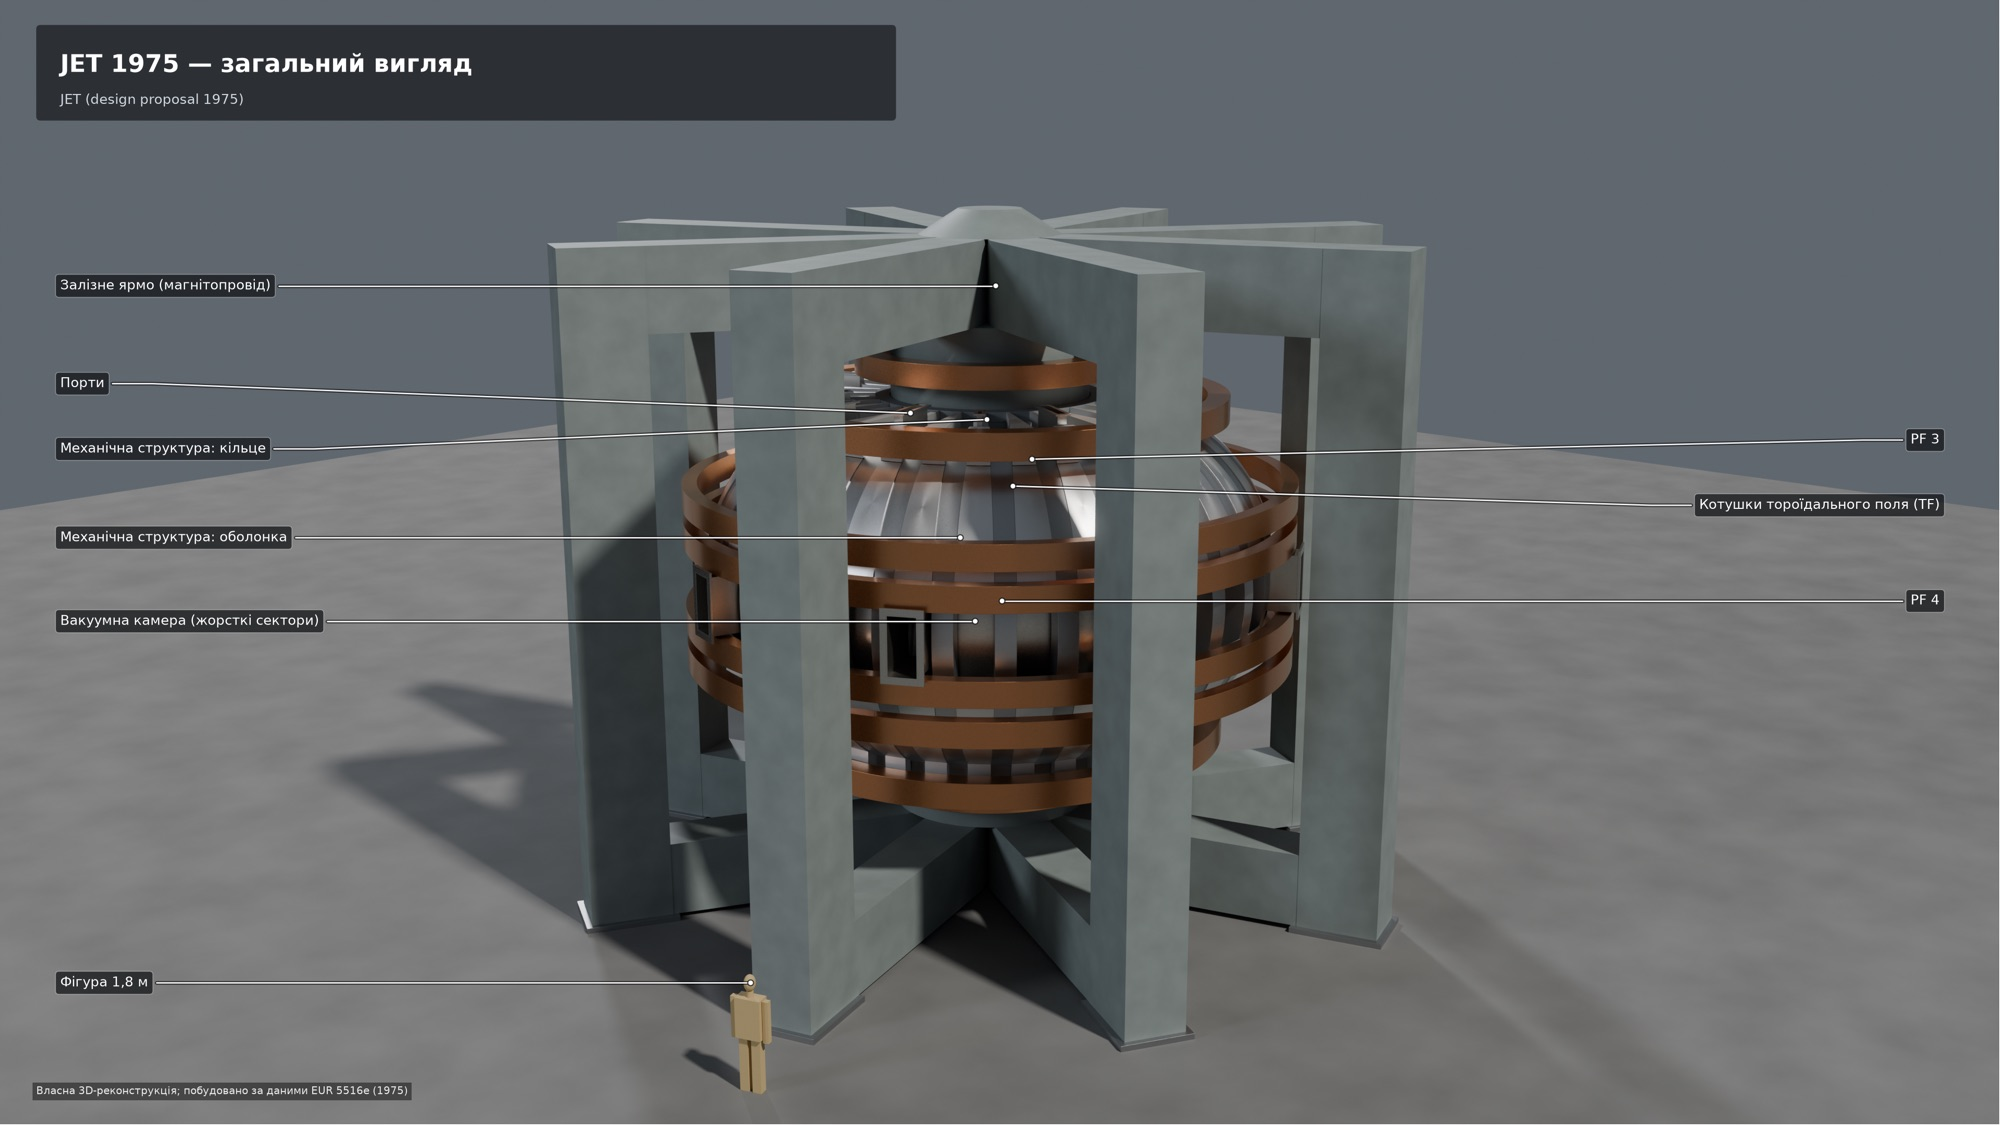
\includegraphics[width=0.8\textwidth]{jet_C1.jpg}
  \caption{JET за проєктом 1975~р.: загальний вигляд. Вісім стрижнів залізного ярма
  (магнітопроводу) охоплюють котушки тороїдального поля (TF), кільцеві котушки
  полоїдального поля (позначено PF\,3 і PF\,4), вакуумну камеру з жорстких секторів,
  механічну структуру (кільце й оболонку) та порти; фігура людини \SI{1.8}{м} --- для
  масштабу. За проєктом зовнішній діаметр машини \SI{14.8}{м}, висота \SI{11.5}{м}~\cite[с.~4]{JET1975};
  плазми ззовні не видно (детально --- розд.~\ref{ch:jet}).
  Власна 3D-реконструкція~\cite{ProjJET}; побудовано за даними~\cite[с.~4, 80, 83]{JET1975}.}
  \label{fig:01-cutaway}
\end{figure}

\section{Токамак, стеларатор і пінч з оберненим полем}\label{sec:01-configs}

\textbf{Токамак} закручує силові лінії струмом плазми, який наводить трансформатор,
тому розряд імпульсний. \textbf{Стеларатори} (зокрема торсатрони й геліотрони) закручують силові
лінії гвинтовими обмотками, тож струм плазми для утримання не потрібен. Торсатрон
Ураган-2М має 16 котушок тороїдального поля, 2 гвинтові та 4 полоїдальні
котушки~\cite{Martsenyuk2025}. Полюс гвинтової обмотки торсатрона Ураган-3 намотано
на тор за законом
$m\tor=-\pol+\alpha_{\mathrm{h}}\sin\pol+\beta_{\mathrm{h}}\sin2\pol$ з $m=3$,
$\alpha_{\mathrm{h}}=0{,}2$, $\beta_{\mathrm{h}}=-0{,}0105$~\cite{Zaitsev2003}, де $m$ --- число обертів обмотки навколо кругової осі тора, а $\alpha_{\mathrm{h}}$ і
$\beta_{\mathrm{h}}$ --- коефіцієнти модуляції (у~\cite{Zaitsev2003} їх позначено $\alpha$, $\beta$).
Симетрія поля впливає й на потоки: спонтанне тороїдальне обертання в геліотронах
спрямоване протилежно до токамачного~\cite{Ida2001} (розд.~\ref{ch:flows}). \textbf{Пінч з оберненим полем} (reversed-field pinch, RFP) має
$\Btor\sim\Bpol$, причому $\Btor$ змінює знак біля краю. Стійкість тут забезпечує
великий шир, а не великий $q$. Merlo~\cite{Merlo2011}, посилаючись на Тейлора, відносить до станів мінімальної енергії за
збереженої спіральності і токамак, і RFP; у стандартній теорії релаксованим станом Тейлора
($\grad\times\Bvec=\lambda\Bvec$, $\lambda=\mathrm{const}$) є саме RFP, а токамак від нього
далекий. RFX-mod у режимі RFP несе до \SI{2}{\mega\ampere}, а в токамачному --- до
\SI{200}{\kilo\ampere}~\cite{Merlo2011}. Перевірте за~\eqref{eq:01-qcyl}: за
$\Btor\le\SI{0.6}{\tesla}$ умова $q(a)\ge3$ виконується лише до $\Ip\approx\SI{105}{\kilo\ampere}$,
тож сильнострумові токамачні розряди RFX-mod мають $q(a)<3$.

\begin{corpusexample}[магнітна система та її межі]
\emph{Котушки TF.} У плоскій багатошаровій котушці TF повне скріплення шарів дає згинальні
напруження з максимумом розтягу в міді \SI{41.6}{\mega\pascal}; часткове роз'єднання
сталевих накладок і провідної частини з пружним опиранням знижує його до
\SI{31.5}{\mega\pascal}~\cite{Zaitsev2001}. \emph{Гвинтова обмотка.} Під час рівномірного
прогріву «безсилової» обмотки Ураган-3 до $T_0\approx\SI{90}{\celsius}$ напруження в сталевій
оболонці сягають \SIrange{130}{140}{\mega\pascal}~\cite{Zaitsev2003}. \emph{Поле як важіль
проєкту.} За сталих $A$, $\kappa$, $\qnf$ і $Q=10$ скейлінг утримання ELMy H-моди дає
$a\propto T^{0{,}51}(G/N)^{0{,}38}B^{-1{,}32}(P_w/N)^{-0{,}02}$~\cite{Mazzucato2000}.
Перерахунок ITER-FEAT ($B=\SI{5.3}{\tesla}$, $a=\SI{2.0}{\metre}$) на \SI{13}{\tesla}
дає $a\approx\SI{0.53}{\metre}$, $R\approx\SI{1.63}{\metre}$. При цьому $n/\nGW$ падає
з 0,85 до 0,39, а $\betaN$ --- з 1,77 до 0,99~\cite{Mazzucato2000}. Ціна --- магніти: надпровідники важко
застосовувати вже за \SI{8}{\tesla}, тож пропонуються кріогенно охолоджені нормальні
провідники~\cite{Mazzucato2000}.
\end{corpusexample}

\section{Установки корпусу}\label{sec:01-devices}

У табл.~\ref{tab:01-devices} --- лише параметри, які джерела наводять \emph{явно}.

\begin{table}[h]
\centering\footnotesize\setlength{\tabcolsep}{4pt}\renewcommand{\arraystretch}{0.92}
\caption{Параметри установок за джерелами корпусу («---» --- у корпусі немає)}\label{tab:01-devices}
\begin{tabular}{@{}lllllll@{}}
\toprule
Установка & Тип & $R_0$, м & $a$, м & $\Bzero$, Тл & $\Ip$, МА & Джерело \\
\midrule
ITER-FEAT (проєкт) & токамак & 6,2 & 2,0 & 5,3 & 15 & \cite{Mazzucato2000,Moskvitina2010} \\
ITER-клас (1992), $\kappa=2$ & токамак & 6 & 2 & 4,85 & 22 & \cite{Fukuyama1992} \\
JET$^{a}$ & токамак & 2,96 / 3 & 1,25 & 2,4 / 3,45 & --- & \cite{Hoppe2022,Fukuyama1992} \\
JET, проєкт 1975$^{h}$ & токамак & 2,96 & 1,25 & 2,77 / 3,45 & 3,8 / 4,8 & \cite[с.~83]{JET1975} \\
ASDEX Upgrade & токамак & 1,65 & 0,5 & 2,5$^{b}$ & 0,8$^{b}$ & \cite{AhoMantila2011} \\
DIII-D \#203702 & токамак & 1,68$^{c}$ & --- & 1,93$^{c}$ & --- & \cite{ProjViz} \\
TFTR & токамак & --- & 0,82$^{d}$ & 4,0$^{d}$ & 0,8--1,8 & \cite{Wong1987,Park1989} \\
NSTX & сфер.\ токамак & 1,0$^{e}$ & 0,85$^{e}$ & 0,45$^{e}$ & 1,0 & \cite{Tyshchenko2021,Jardin2000} \\
JFT-2M & токамак & --- & --- & --- & 0,243 & \cite{Ida2001} \\
WT-3 & токамак & 0,65 & 0,20 & $\le1{,}75$ & $\le0{,}15$ & \cite{Hanada1990} \\
T-10 & токамак & 1,5 & 0,28--0,30 & 1,6--2,4 & 0,20--0,33 & \cite{Marchuk2025} \\
EAST & токамак & 1,86 & 0,45 & 2,0 & 0,25 & \cite{Marchuk2025} \\
RFX-mod & RFP/токамак & 2,0 & 0,459$^{f}$ & $\le0{,}6$ & $\le2$ / $\le0{,}2$ & \cite{Merlo2011} \\
Ураган-2М & торсатрон & 1,7 & $<0{,}24$ & $<2{,}4$ & --- & \cite{Martsenyuk2025} \\
Ураган-3 & торсатрон & 1,0$^{g}$ & --- & --- & --- & \cite{Zaitsev2003} \\
\bottomrule
\end{tabular}\\[2pt]
\parbox{\textwidth}{\footnotesize $^{a}$~перше число --- сценарій пуску (прогоряння)~\cite{Hoppe2022}, друге --- розряд 1992~р.~\cite{Fukuyama1992} ($a=1{,}25\times2{,}1$~м);
$^{b}$~розряд на рис.\ у~\cite{AhoMantila2011}; $^{c}$~$R$ магнітної осі та відкаліброване
$\Btor$ на осі, $\qnf=3{,}70$; $^{d}$~модельні значення, $\Ip=\SI{0.7}{\mega\ampere}$
у~\cite{Wong1987}; $^{e}$~модельні значення в~\cite{Tyshchenko2021}; $^{f}$~радіус першої
стінки; $^{g}$~радіус обмотки (її внутрішній малий радіус \SI{0.203}{\metre}). $^{h}$~базовий / розширений варіант, D-подібна плазма з $b=\SI{2.10}{м}$ і $q(a)=6$
(детально --- розд.~\ref{ch:jet}). $T$, $n_e$, $q$ для AUG, JET, ITER
див. у табл.~I~\cite{vanVugt2019}.}
\end{table}

\subsection*{Контрольні запитання}
\begin{enumerate}
  \item Звідки в $G$ число 5? Чому дорівнювало б $G$, якби нейтрона не було?
  \item Чому чисто тороїдальне поле не утримує плазму? Як це долають токамак і стеларатор?
  \item Чому з $q(a)\ge3$ за $R_0/a\approx3$ випливає $\Btor\gg\Bpol$? Як без цього обходиться RFP?
  \item Що означає раціональне $q=m/n$ для силової лінії і чому такі поверхні особливі?
  \item Чому підвищення $\Bzero$ зменшує розмір установки з $Q=10$ і що обмежує $\Bzero$ згори?
\end{enumerate}

\subsection*{Задачі}
\begin{enumerate}
  \item ITER-FEAT: $Q=10$, $P_{\mathrm{fus}}=\SI{410}{\mega\watt}$~\cite{Mazzucato2000}. Знайдіть
        $P_\alpha$, $P_{\mathrm{ext}}$, $G$ і повну потужність нагріву; порівняйте з
        $P_{LH}=\SI{48}{\mega\watt}$ з тієї ж таблиці.
  \item Оцініть $q(a)$ за~\eqref{eq:01-qcyl} для WT-3 за максимальних $\Bzero$ і
        $\Ip$~\cite{Hanada1990}. Чи лежить він у діапазоні $q_L=2{,}2$--$6{,}0$, де там
        бачили пилкоподібні коливання? За якого $\Ip$ було б $q(a)=3$?
  \item Скейлінг~\cite{Mazzucato2000}: знайдіть $a$ за сталих $G$, $N$ для переходу ITER-FEAT
        (\SI{5.3}{\tesla}, \SI{9}{\kilo\electronvolt}, $P_w=\SI{0.5}{\mega\watt\per\square\metre}$) $\to$
        (\SI{13}{\tesla}, \SI{7}{\kilo\electronvolt}, \SI{1.5}{\mega\watt\per\square\metre}).
\end{enumerate}

\chapter{Рух заряджених частинок у полі токамака}\label{ch:particles}

Рідинні моделі наступних розділів усереднюють рух окремих частинок; тут розглянемо одну частинку (заряд $e_s$, маса $m_s$) у заданих $\vect{E}$, $\Bvec$; $\Omc{s}=e_sB/m_s$, ларморів радіус $\rho_s=v_\perp/|\Omc{s}|$.

\section{Рівняння Лоренца і чисельні інтегратори}\label{sec:02-lorentz}

Без зіткнень рух описується рівнянням Ньютона з силою Лоренца (переведено з СГС~\cite{Moskvitina2010}):
\begin{equation}\label{eq:02-lorentz}
  m_s\,\dot{\vect{v}} = e_s\left(\vect{E}+\vect{v}\times\Bvec\right),\qquad \dot{\vect{r}}=\vect{v}.
\end{equation}
Для МеВ-іонів $\rho_s\sim\SI{10}{см}$, тому дрейфове наближення (п.~\ref{sec:02-gc}) стає неточним, і потрібні коди повної орбіти (full-orbit codes)~\cite{Moskvitina2010}.

\textbf{Схема Боріса (Boris pusher).} Швидкості задано в півкроках, координати~--- у цілих кроках (схема типу leap-frog)~\cite{vanVugt2019}:
\begin{equation}\label{eq:02-boris}
  \frac{\vect{v}^{n+1/2}-\vect{v}^{n-1/2}}{\Delta t}=\frac{e_s}{m_s}\left[\vect{E}+\frac{\vect{v}^{n+1/2}+\vect{v}^{n-1/2}}{2}\times\Bvec\right].
\end{equation}
Підстановка
\[
  \vect{v}^{n\pm1/2}=\vect{v}^{\pm}\pm\frac{e_s\Delta t}{2m_s}\,\vect{E}
  \quad\Longrightarrow\quad
  \vect{v}^{+}-\vect{v}^{-}=\frac{e_s\Delta t}{2m_s}\,(\vect{v}^{+}+\vect{v}^{-})\times\Bvec
\]
повністю виключає $\vect{E}$ і лишає чистий поворот вектора, тож $|\vect{v}|$ у магнітному полі зберігається точно на кожному кроці. Заміна $f=e_s\Delta t/(2m_s)$ на $f'=\tan(f|\Bvec|)/|\Bvec|$ робить частоту обертання точно циклотронною~\cite{vanVugt2019}. Для іонів W у JOREK (ASDEX Upgrade) потрібно $\Delta t\lesssim\SI{e-8}{с}$, взято \SI{e-9}{с}~\cite{vanVugt2019}.

\begin{corpusexample}[РК4 проти РК5 для α-частинки в ITER]
\noindent\begin{minipage}[c]{0.53\linewidth}
Москвитина~\cite{Moskvitina2010} порівнює класичну схему Рунге--Кутти 4-го порядку (РК4) і шеститочкову схему 5-го порядку (РК5) на α-частинці \SI{1}{МеВ}, $v_\parallel/v=0{,}1$, за $1000\,T_c$ ($T_c\approx\SI{2,48e-8}{с}$). Мірою точності є $\delta=\Delta E/E_0$ (без $\vect{E}$ енергія~--- інваріант).
\end{minipage}\hfill
\begin{minipage}[c]{0.44\linewidth}\centering\small
\begin{tabular}{@{}lccc@{}}
\toprule
Схема & $h/T_c$ & $\delta$ & $t_{\mathrm{CPU}}$, с \\
\midrule
РК5 & $10^{-2}$ & $\approx10^{-9}$ & 2,22 \\
РК4 & $10^{-2}$ & $\approx10^{-4}$ & 1,45 \\
РК4 & $10^{-3}$ & $\approx10^{-9}$ & 15,17 \\
\bottomrule
\end{tabular}
\end{minipage}\par\smallskip
За однакової точності РК4 повільніша в $6{,}8$ раза («у 7 разів» у статті). Обидві схеми насичуються на $\delta\approx10^{-12}$ (подвійна точність); порівняння з Борісом у статті немає.
\end{corpusexample}

\section{Ведучий центр і дрейфи}\label{sec:02-gc}

\begin{outofcorpus}[дрейфове наближення]
Нехай $\rho_s\ll L$ (масштаб неоднорідності) і $\omega\ll\Omc{s}$. Розкладемо $\vect{r}=\vect{X}+\vect{\rho}$, де $\vect{X}$~--- ведучий центр (guiding centre), а $\vect{\rho}$ обертається з фазою $\Theta$. Усереднивши \eqref{eq:02-lorentz} за $\Theta$ при сталій сторонній силі $\vect{F}_\perp$, дістанемо дрейф
\begin{equation}\label{eq:02-Fdrift}
  \vect{v}_F=\frac{\vect{F}\times\Bvec}{e_sB^2}.
\end{equation}
\emph{(а)} $\vect{F}=e_s\vect{E}$: $\vE=\ExB/B^2$ однаковий для всіх сортів, і струму він не несе. \emph{(б)} Усереднена сила на ларморове кільце в неоднорідному полі $\vect{F}=-\mu\grad B$, де $\mu=m_sv_\perp^2/(2B)$~--- магнітний момент: $\vect{v}_{\grad B}=\frac{m_sv_\perp^2}{2e_sB}\frac{\unitb\times\grad B}{B}$. \emph{(в)} Відцентрова сила при русі вздовж викривленої лінії $\vect{F}=-m_sv_\parallel^2\vect{\kappa}$, $\vect{\kappa}=\unitb\cdot\grad\unitb$: $\vect{v}_\kappa=\frac{m_sv_\parallel^2}{e_sB}\,\unitb\times\vect{\kappa}$. У полі з малим $\beta$ ($\grad\times\Bvec\approx0$) $\vect{\kappa}=\grad_\perp B/B$, і
\begin{equation}\label{eq:02-vd}
  \vect{v}_d=\frac{m_s}{e_sB}\Bigl(v_\parallel^2+\tfrac12v_\perp^2\Bigr)\frac{\unitb\times\grad B}{B}\;\approx\;\frac{m_s\bigl(v_\parallel^2+\tfrac12v_\perp^2\bigr)}{e_sRB}\,\hat{\vect{Z}}\quad(B\propto1/R,\ \Btor>0).
\end{equation}
Дрейф вертикальний і має різні знаки для іонів та електронів (для $\Btor>0$ іони дрейфують угору). У чисто тороїдальному полі розділення зарядів створює $E_Z$, і дрейф $\vE$ викидає плазму назовні. Полоїдальне поле (обертальне перетворення, $q$) переносить частинку то вгору, то вниз, і вертикальний дрейф усереднюється до нуля.
\end{outofcorpus}

Зв'язок з корпусом. (1)~Радіальну компоненту дрейфу в нормованому потоці $v_{\psiN}=(\ExB)\cdot\grad\psiN/B^2$ у~\cite{vanVugt2019} (рівн.~8) обчислено з полів ELM і порівняно з рухом іонів W. Швидкості $|v_{\psiN}|$ сягають \SI{5000}{с^{-1}}, тобто тисячі одиниць $\psiN$ за секунду (перетин малого радіуса за \SI{0,2}{мс}); розподіл симетричний. Без $\delta\vect{E}$ радіального переносу немає, без $\delta\Bvec$~--- є: W переносить саме $\vE$. (2)~У гірокінетичному коді GTC ведучі центри рухаються вздовж $\hat{\vect{b}}^*=\unitb+\rho_\parallel\unitb\times(\unitb\cdot\grad\unitb)$ з дрейфами $\vect{v}_{E_0}$, $\vE$, $\vect{v}_d$~\cite{Wang2006} (рівн.~13). (3)~Частота прецесії швидких електронів $\omega_{de}=W_\perp/(e\,rR\Bzero)$ ($W_\perp$~--- поперечна енергія)~\cite{Hanada1990}~--- це дрейф \eqref{eq:02-vd} при $v_\parallel\to0$, поділений на $r$; умова $\omega_{de}>\omega_{*e}/2$ на WT-3 дає $W_\perp\gtrsim T_eR/a\approx\SI{1,5}{кеВ}$.

\section{Пролітні й захоплені частинки, бананові орбіти}\label{sec:02-banana}

\begin{outofcorpus}[захоплення і ширина банана]
На поверхні $r$ поле $B\approx\Bzero(1-\varepsilon\cos\theta)$, де $\varepsilon=\varepsilon(r)=r/R_0$ (локальне). Збереження $\mu$ і $E$ дає $v_\parallel^2=v^2-2\mu B/m_s$. Частинка з $(v_{\parallel0},v_{\perp0})$ на зовнішньому обводі ($\theta=0$) відбивається, якщо
$v_{\parallel0}^2/v_{\perp0}^2<B_{\max}/B_{\min}-1=2\varepsilon/(1-\varepsilon)$.
Частка захоплених становить $f_t\sim\sqrt{2\varepsilon}$. Ширину орбіти дає осесиметрія: канонічний тороїдальний момент
\begin{equation}\label{eq:02-Pphi}
  p_\varphi=m_sRv_\varphi+e_s\psi=\mathrm{const}
\end{equation}
(ψ~--- потік на радіан, $A_\varphi=\psi/R$). Між двома проходами площини $\theta=0$ з $v_\parallel=\pm v_{\parallel0}$ маємо $\Delta\psi=2m_sRv_{\parallel0}/e_s$, $\Delta r=\Delta\psi/(R\Bpol)$, тож
\begin{equation}\label{eq:02-wb}
  w_{\mathrm b}\approx\frac{2m_sv_{\parallel0}}{e_s\Bpol}=\frac{2q\,v_{\parallel0}}{\varepsilon\,\Omc{s}}\sim\frac{2\sqrt2\,q\,\rho_s}{\sqrt{\varepsilon}}.
\end{equation}
Порушення осесиметрії (гофрування, п.~\ref{sec:02-ripple}) руйнує \eqref{eq:02-Pphi}, і орбіта перестає бути замкненою.
\end{outofcorpus}

\begin{corpusexample}[банани в корпусі]
\emph{ITER}: РК5-траєкторія α-частинки \SI{3,5}{МеВ}, $v_\parallel/v=0{,}1$, є «бананом» з періодом баунс-коливань $\tau_b=687\,T_c\approx\SI{1,7e-5}{с}$~\cite{Moskvitina2010}. \emph{Важкі домішки}: табл.~I у~\cite{vanVugt2019} дає для W в ядрі $\rho_s=\SIlist{1,1;1,5;1}{мм}$ і ширину банана $w_{\mathrm b}=\SIlist{40;60;10}{мм}$ (ASDEX Upgrade, JET, ITER). Відношення $w_{\mathrm b}/\rho_s\sim10$--$40$ узгоджується з \eqref{eq:02-wb}. \emph{Швидкі електрони} ECH з боку слабкого поля захоплюються на банани і не несуть струму~--- звідси асиметрія HFS/LFS стабілізації пилки на WT-3~\cite{Hanada1990}.
\end{corpusexample}

\section{Гофрування тороїдального поля}\label{sec:02-ripple}

Скінченне число котушок $N_{\mathrm{TF}}$ робить поле періодичним по $\varphi$. У моделі~\cite{Moskvitina2010} (кругові поверхні, квазітороїдальні $(r,\theta,\varphi)$) $\Bvec=\Bvec^0+\Bvec^1$, $\Bvec^0=\frac{\Bzero R_0}{R_0-r\cos\theta}\bigl(0,\frac{r}{qR_0},1\bigr)$ і
\begin{equation}\label{eq:02-ripple}
  B^1_\varphi=\Bzero\,2k a_{\mathrm{TF}}K_1(ka_{\mathrm{TF}})\,I_0(kr)\cos(N_{\mathrm{TF}}\varphi),
\end{equation}
$B^1_\theta=0$, а $B^1_r\propto I_0'(kr)\sin(N_{\mathrm{TF}}\varphi)$ забезпечує $\grad\cdot\Bvec^1=0$. Тут $K_1$, $I_0$~--- модифіковані функції Бесселя (Макдональда і Бесселя), $a_{\mathrm{TF}}$~--- радіус котушок. Для ITER $a=\SI{2,0}{м}$, $R_0=\SI{6,2}{м}$, $a_{\mathrm{TF}}=\SI{4,0}{м}$, $\Bzero=\SI{5,3}{Тл}$, $k=\SI{2,9}{м^{-1}}$ (переведено з СГС)~\cite{Moskvitina2010}. Глибина гофрування $\dripple(r)=B^1_\varphi/\Bzero$ за \eqref{eq:02-ripple} становить $8{,}1\cdot10^{-5}$ на осі і $4{,}5\cdot10^{-3}$ при $r=a$ (наш розрахунок): вона зростає до краю експоненційно, як $I_0(kr)$.

У JET тороїдальне поле створюють 32 D-подібні котушки~\cite[с.~77]{JET1975}, і проєкт 1975~р.
задає гофрування \SI{3.6}{\percent} на зовнішньому краю плазми~\cite[с.~83]{JET1975}. Увага до
означення: у проєкті $\eripple=2(B_{\max}-B_{\min})/(B_{\max}+B_{\min})$~\cite[с.~330]{JET1975},
тобто це розмах, удвічі більший за амплітуду $\dripple$ з~\eqref{eq:02-ripple}. Наша
реконструкція котушок за Біо--Саваром дає $\eripple=\SI{3.67}{\percent}$ при
$R=\SI{4.21}{м}$ (невизначеність близько $\pm13\,\%$ через оцифровану форму котушки)~\cite{ProjJET};
порівнюючи числа різних джерел, завжди з'ясовуйте, яке з двох означень ужито
(детально --- розд.~\ref{ch:jet}).

\begin{outofcorpus}[гофрувальні втрати]
Частинки з малим $v_\parallel$ захоплюються в локальні ями вздовж $\varphi$ і без компенсації дрейфують \eqref{eq:02-vd} до стінки (ripple trapping); точки відбиття бананів випадково зсуваються, що дає стохастичну дифузію. Обидва механізми найсильніші для швидких іонів на периферії.
\end{outofcorpus}

\section{Обертова система відліку}\label{sec:02-rot}

Нехай поверхні обертаються як жорсткі оболонки з $\omtor(r)$. У системі, що обертається з плазмою, силові лінії нерухомі, а рівняння руху домішки (заряд $Z_Ie$, маса $m_I$) набуває сил Коріоліса і відцентрової~\cite{Wong1987}:
\begin{equation}\label{eq:02-rot}
  m_I\dot{\vect{v}}=Z_Ie(\vect{E}+\vect{v}\times\Bvec)-2m_I\,\vect{\omega}\times\vect{v}-m_I\,\vect{\omega}\times[\vect{\omega}\times(\vect{R}_0+\vect{r})],\qquad \vect{\omega}=\omtor\hat{\vect{Z}}.
\end{equation}
Кожна нова сила дає свій дрейф \eqref{eq:02-Fdrift}: рівн.~(4) у~\cite{Wong1987}~--- це \eqref{eq:02-vd} з доданками Коріоліса й відцентровим. Відцентрова сила відтискає іони на зовнішній обвід, і квазінейтральність підтримує полоїдально змінний потенціал~\cite{Wong1987}
\begin{equation}\label{eq:02-Phi1}
  \Phi_1=\frac{\omtor^2}{2}\,\frac{m_i}{e}\,\frac{T_e}{T_i+Z_iT_e}\,\bigl(R^2-\fsa{R^2}\bigr).
\end{equation}
(таку саму складову $\tilde\Phi_0$ має рівноважний потенціал GTC~\cite{Wang2006}). Межа захоплення в просторі швидкостей стає гіперболічною поверхнею, у яку входять $\omtor^2$ і різниця $\Phi$ між максимумом і мінімумом $R$ на поверхні~\cite{Wong1987}. При $m_I\omtor^2R^2\gg T_I$ майже всі важкі іони захоплені. Для TFTR ($\Btor=\SI{4}{Тл}$, $\omtor(0)=\SI{2e5}{рад/с}$, $n_e(0)=\SI{2e19}{м^{-3}}$, $T_i(0)=\SI{10}{кеВ}$, $a=\SI{0,82}{м}$; переведено з СГС) банани домішок мають ширину кілька сантиметрів, а $D_{\mathrm{neo}}$ германію на 1--2 порядки більший, ніж без обертання, близький до потрібних $\SI{3}{м^2/с}$~\cite{Wong1987}. Як обертання формує радіальне поле й потоки, розглянуто в розд.~\ref{ch:flows}.

\section{Гамільтонів опис силових ліній і магнітні острови}\label{sec:02-ham}

Тищенко~\cite[с.~40--41]{Tyshchenko2021} зводить диференціальну форму ведучого центру в магнітних координатах до $\Gamma=J\,\dd\thetastar-\mathcal{H}\,\dd\varphi$, $J=\psit/\Bzero$. Тут $\psit=\Psit/2\pi$~--- тороїдальний потік \emph{на радіан} (у~\cite{Tyshchenko2021}~--- $\psi$; $J$~--- площа перерізу поверхні, поділена на $2\pi$). У одиницях потоку, з амплітудою $\tilde\psi_{mn}=\Bzero R_0^2\alpha$ замість її $\alpha$ (переведено з СГС) і $\rho_\parallel=v_\parallel/\Omc{s}$,
\begin{equation}\label{eq:02-H}
  \Bzero\mathcal H=\psi(\psit)-\rho_\parallel R_0\Bzero+\tilde\psi_{mn}(\psit)\cos(m\thetastar-n\varphi),\qquad
  \frac{\dd\thetastar}{\dd\varphi}=\frac{\pa\mathcal H}{\pa J},\quad\frac{\dd J}{\dd\varphi}=-\frac{\pa\mathcal H}{\pa\thetastar}.
\end{equation}
Усі доданки мають розмірність потоку (\si{\tesla\metre\squared}), а $\mathcal H$ і $J$~--- площі (з потоками на радіан зайвих множників $2\pi$ немає). Кут $\thetastar$~--- координата, $\psit$~--- імпульс, полоїдальний потік $\psi$~--- гамільтоніан (з точністю до знака конвенції), $\varphi$~--- час. Чому гамільтоніаном є саме $\psi$, видно з поля в магнітних координатах $\Bvec=\grad\psit\times\grad\thetastar+\grad\tor\times\grad\psi$ (з точністю до знака): оскільки $\grad\psit=q\grad\psi$, чисельник і знаменник у
\[
  \frac{\dd\thetastar}{\dd\tor}=\frac{\Bvec\cdot\grad\thetastar}{\Bvec\cdot\grad\tor}=\frac{\dd\psi}{\dd\psit}=\frac1q
\]
містять той самий мішаний добуток $\grad\tor\cdot(\grad\psi\times\grad\thetastar)$, тож $\dd\thetastar/\dd\tor=\pa\psi/\pa\psit$~--- перше рівняння Гамільтона. При $\rho_\parallel=0$ \eqref{eq:02-H} описує силові лінії, при $\rho_\parallel\ne0$~--- ведучий центр пролітної частинки. Тищенко прямо зазначає, що одна мода при $\rho_\parallel=0$ хаосу не дає: у магнітних координатах гамільтоніан однієї моди залежить лише від гвинтової фази, тож система інтегровна~\cite{Tyshchenko2021}.

\begin{figure}[t]
  \centering
  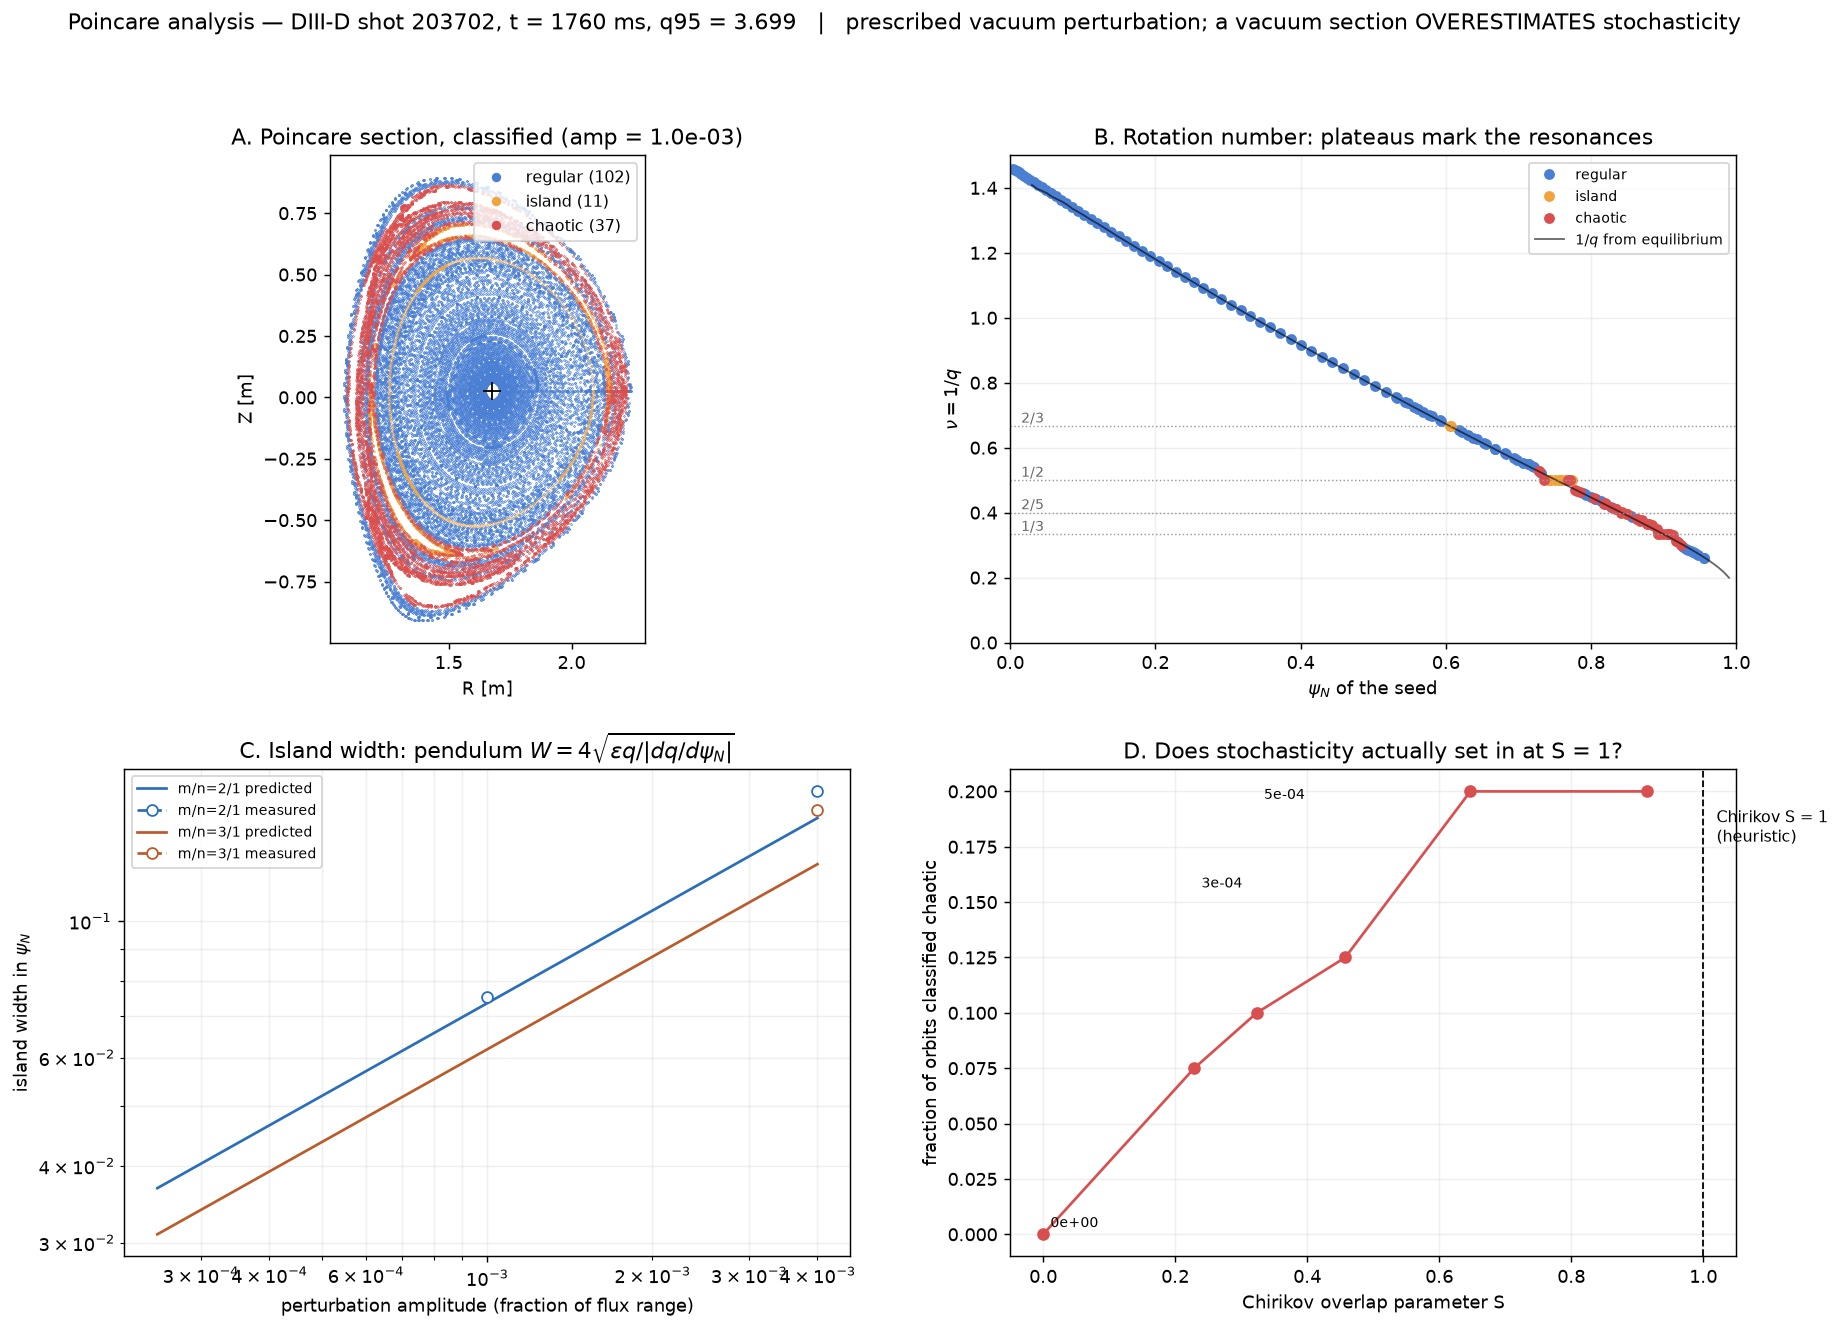
\includegraphics[width=0.88\textwidth,trim=0 0 0 55,clip]{poincare_analysis_fixed.jpg}
  \caption{Переріз Пуанкаре DIII-D \#203702 ($t=\SI{1760}{мс}$, $\qnf=3{,}699$) з вакуумними модами 2/1 і 3/1, прогін після виправлення формули ширини (29.09.2026): A~--- класифіковані орбіти (амплітуда $10^{-3}$); B~--- $\nu=1/q$ з трасування і з рівноваги; C~--- виміряна $w_{mn}$ (кружки) проти маятникової формули~\eqref{eq:02-w} (лінії; в $\psiN$-одиницях); D~--- частка хаотичних орбіт проти $S$: жодна амплітуда скану не досягає $S=1$, а хаотичні орбіти є вже при $S\approx0{,}23$. Власний розрахунок~\cite{ProjViz}; дані рівноваги: Fusion Equilibrium Challenge (Sophelio / General Atomics), CC BY 4.0.}
  \label{fig:02-poincare}
\end{figure}

\begin{established}{E18--E20}
В осесиметрії ($\tilde\psi_{mn}=0$) $\Bvec\cdot\grad\psi=0$, система інтегровна, і переріз Пуанкаре~--- рівно контури ψ~\cite{ProjRegisters}. У \texttt{tokamak-3d-viz} це юніт-тест: дрейф ψ уздовж лінії за 200 обертів, $\max|\Delta\psi|/|\psib-\psiax|$ (тобто в одиницях $\psiN$), становить $10^{-7}$--$1{,}4\cdot10^{-6}$~\cite{ProjViz}. Острови з EFIT не виникають~--- їх вносять збуренням. \textbf{E19:} канонічний словник силових ліній: час~--- φ, координата~--- θ, імпульс~--- \emph{тороїдальний} потік, гамільтоніан~--- \emph{полоїдальний}~\cite{ProjRegisters}; таку структуру має \eqref{eq:02-H}~\cite{Tyshchenko2021}. \textbf{E20:} одна резонансна мода дає острови, але не хаос: у гвинтовому куті $m\thetastar-n\varphi$ система інтегровна~\cite{ProjRegisters,Tyshchenko2021}; хаос вимагає кількох мод, що перекриваються.
\end{established}
\begin{established}{E39 (прочитано й перевірено)}
Обернене до E18 хибне: вкладені магнітні поверхні можливі й без осесиметрії. Landreman~\cite{Landreman2026} дав явні гладкі тороїдальні 3D-рівноваги МГД з $\grad p\ne0$ і відхиленням від осесиметрії порядку одиниці. Рівняння статті перевірено власним кодом проєкту до $10^{-10}$--$10^{-12}$, помилок не знайдено. Застереження: в одного з двох сімейств саме поле $\Bvec$ має точну неізометричну симетрію (лінійний образ поля Соловйова), яку порушують $|\Bvec|$, густина струму й тиск~\cite{ProjRegisters}.
\end{established}
\begin{refuted}{R4}
«ψ~--- канонічний імпульс». Неправильно: імпульс~--- $\psit$, а ψ~--- гамільтоніан~\cite{ProjRegisters}. Ця помилка не лише термінологічна. Хто вважає ψ імпульсом, той у формулі ширини острова отримує зайвий множник $\sqrt q$ (див. нижче). Саме цю помилку мав код \texttt{tokamak-3d-viz} до 29.09.2026 (VR15~\cite{ProjViz}).
\end{refuted}

\begin{derivation}[ширина острова]
Поблизу $q(\psi_{\mathrm{t},r})=m/n$ перейдемо до гвинтового кута $\xi=m\thetastar-n\varphi$ (твірна функція $F_2=\xi P$, $\psit=mP$): $K=\psi(mP)-nP+\tilde\psi_{mn}\cos\xi$. Розклад до другого порядку за $\Delta P$ дає маятник $K\approx\tfrac12m^2\psi''\Delta P^2+\tilde\psi_{mn}\cos\xi$, $\psi''=-q'/q^2$. Повна ширина сепаратриси в $\psit$ дорівнює $4\sqrt{\tilde\psi_{mn}q^2/|\dd q/\dd\psit|}$. Оскільки $\dd\psit=q\,\dd\psi$, у полоїдальному потоці
\begin{equation}\label{eq:02-w}
  w_{mn}=4\sqrt{\frac{\tilde\psi_{mn}\,q}{|\dd q/\dd\psi|}}\,.
\end{equation}
$m$ скорочується. Те саме дає пряме рівняння $\dd\psi/\dd\varphi=-q^{-1}\pa\tilde\psi/\pa\thetastar$. Перекриття сусідніх ланцюгів оцінює параметр Чирикова $S=(w_1+w_2)/(2|\psi_1-\psi_2|)$; $S\gtrsim1$~--- евристика, а не теорема.
\end{derivation}

\begin{established}{E30--E32 (D3)}
Tokamap (Balescu--Vlad--Spineanu) \emph{точно симплектичний}: якобіан мапи $\mathsf D$: $\max|\det\mathsf D-1|=5{,}6\cdot10^{-8}$ (E30). Спостережувана з однієї початкової фази непридатна: рівень шуму $0{,}3244$, а з усередненням по 24 фазах~--- $0{,}0006$ (E31; застереження реєстру: два рівні виміряно на різних стендах --- тримодовій несимплектичній мапі й одномодовій Tokamap, тож їхнє відношення не є чистою мірою усереднення). Одну амплітуду $x_L$ відновити тривіально: зміна на 3\,\% дає SNR 57 (E32)~\cite{ProjRegisters,ProjDeepDives}.
\end{established}
\begin{refuted}{R8}
«Структуру Tokamap можна перенести на суму мод підстановкою $V'(T)$». Симплектичність ламається: $\max|\det\mathsf D-1|=1{,}7$ при амплітуді $0{,}5$. Така мапа не зберігає потік і не є відображенням силових ліній~\cite{ProjRegisters,ProjDeepDives}.
Корінь знайдено згодом (E35): поправка до $T'$ має брати первісну $h(T)$ з коефіцієнтами $a_k/m_k$, а не $V'(T)$ з $a_k m_k$ (різниця $m_k^2$); з виправленням $\max|\det\mathsf D-1|=3{,}6\cdot10^{-7}$ при амплітуді $0{,}5$~\cite{ProjRegisters}. Спростоване твердження лишається спростованим.
\end{refuted}
\begin{refuted}{R13 (була гіпотеза C5)}
«Обернена задача „переріз Пуанкаре $\to$ спектр $(m,n)$“ розв'язна за 48~год зі starter kit». Перевірено 2026-10-01 за критеріями, записаними до запуску: базовий багатостартовий нелінійний МНК відновлює 3 амплітуди і 3 фази з фазово-роздільної екскурсії при 3\,\% шуму. На виправленій багатомодовій Tokamap (E35) успіхів 0 з 40, на стенді \texttt{tokamak-3d-viz} (DIII-D \#203702, моди 2/1, 5/2, 3/1)~--- 0 з 3. Хибних мінімумів немає, тож інформація в даних є, але жоден старт не дійшов до рівня шуму~\cite{ProjRegisters,ProjDeepDives}. Спростовано для базового розв'язувача, а не «нерозв'язно».
\end{refuted}
\begin{established}{E40}
Ландшафт нев'язки екскурсійного спостережуваного «скляний». Екскурсія~--- розмах $\max-\min$ по дискретних точках орбіти, тож малий зсув параметра змінює, яка точка дає екстремум, і нев'язка стрибає. Старт в істині лишається на місці, а старт з істини $+5\,\%$ і $+10^\circ$ зупиняється в нев'язці, у 41--100 разів більшій за істинну; уздовж однієї фази в межах $\pm20^\circ$ є 8 локальних мінімумів~\cite{ProjRegisters,ProjGuide}. \emph{Студенту:} замінити розмах гладшою величиною (середнє чи квантиль по орбіті) і перевірити, чи зникнуть локальні мінімуми (\texttt{Our try/03-deep-dives/D3-poincare-inverse/c5/}); критерії записати до запуску.
\end{established}

\begin{practicum}[острови в DIII-D \#203702, \texttt{tokamak-3d-viz}]
\textbf{1.} \texttt{python src/run\_bake.py --out data/bake01 --modes 2/1,3/1 --amp 1e-3} (потрібен \texttt{TOKVIZ\_DATA\_DIR} з parquet). Лог дає резонанси $\psiN=0{,}752$ ($q=2$) і $0{,}900$ ($q=3$), амплітуди, $\dd q/\dd\psiN$, ширини $w_{mn}$ і $S=0{,}458$ (\texttt{perturbation.py}). Збережений \texttt{data/bake01} перепечено 29.09.2026 з виправленою формулою: $w_{21}=0{,}0736$, $w_{31}=0{,}0619$, $S=0{,}458$; орбіти регулярні\,/\,в островах\,/\,хаотичні --- 41\,/\,12\,/\,15 (до виправлення 39\,/\,18\,/\,7).
\textbf{2.} \texttt{python src/run\_analysis.py --out data/analysis} будує рис.~\ref{fig:02-poincare}. \textbf{Історія однієї помилки.} До 29.09.2026 код (\texttt{island\_width\_psin}) брав $w_{mn}=4\sqrt{\tilde\psi_{mn}q^2/|\dd q/\dd\psi|}$ (ψ як імпульс, R4) і завищував ширину в $\sqrt q$ разів; виміряна ширина виходила «замалою» (0,59--0,74 від теоретичної, тобто $1/\sqrt3$--$1/\sqrt2$), а документація пояснювала це стохастичним шаром сепаратриси. Формулу виправлено за~\eqref{eq:02-w}: трасування однієї моди (тест \texttt{test\_island\_width\_matches\_traced\_separatrix} у \texttt{tests/test\_physics.py}) дає відношення виміряної ширини до теоретичної $0{,}983$ (2/1) і $0{,}996$ (3/1); перерахунок збереженого прогону --- $0{,}95$--$1{,}02$; теоретичні $w_{21}=0{,}1041\to0{,}0736$, $w_{31}=0{,}1072\to0{,}0619$, $S=0{,}714\to0{,}458$. Обидва хибні твердження зареєстровано як спростовані: VR15 (формула) і VR16 (пояснення стохастичним шаром)~\cite{ProjViz}. \emph{Завдання:} відтворіть відношення з іншими \texttt{--amps}; покажіть, що при амплітуді $4\cdot10^{-3}$ (край, $S\approx0{,}9$) маятникова формула перестає працювати (відношення 1,1--1,3). Застереження: при новому засіві класифікатор островів (тест пласкості $\nu$) ненадійний (VQ4~\cite{ProjViz}). \textbf{3.} E30--E32: \texttt{tokamap.py}, \texttt{identifiability.py} у \texttt{Our try/03-deep-dives/D3-poincare-inverse}.
\end{practicum}

\subsection*{Контрольні запитання}
\begin{enumerate}
  \item Чому схема Боріса зберігає $|\vect{v}|$ у магнітному полі точно, а РК4 накопичує похибку енергії?
  \item Виведіть \eqref{eq:02-vd} з \eqref{eq:02-Fdrift}. Чому $v_\parallel^2$ входить у дрейф з вагою 1, а $v_\perp^2$~--- з вагою $1/2$?
  \item Звідки береться $\Phi_1$ \eqref{eq:02-Phi1}? Чому $D_{\mathrm{neo}}$ не залежить від знака обертання~\cite{Wong1987}?
  \item Чому одна мода не дає хаосу (E20) і як помилка R4 змінює ширину острова?
\end{enumerate}

\subsection*{Задачі}
\begin{enumerate}
  \item (Москвитина~\cite{Moskvitina2010}.) Для α (\SI{5,3}{Тл}) знайдіть $T_c$, $\rho_\alpha$ при \SI{3,5}{МеВ}, $\tau_b$ у секундах і число кроків РК5 ($h=10^{-2}T_c$) на баунс.
  \item За \eqref{eq:02-ripple} з параметрами ITER обчисліть $\dripple$ при $r=0$; \SI{1}{м}; \SI{2}{м} і перевірте, що $kR_0\approx18$.
  \item (Wong--Cheng~\cite{Wong1987}.) TFTR: $\omtor\propto(1+4r^2/a^2)^{-1}$ (отже, $\omtor(a/2)=\omtor(0)/2$), $T_{e,i}\propto(1+9r^2/a^2)^{-1}$, $T_e(0)=\SI{4}{кеВ}$, $m_{\mathrm{Ge}}=72{,}6$~а.о.м. Для D ($Z_i=1$) і $R_0=\SI{2,5}{м}$ ($R_0$ у~\cite{Wong1987} не наведено; типове значення TFTR) оцініть $\Phi_1$ при $r=a/2$; порівняйте $m_{\mathrm{Ge}}\omtor^2R_0^2$ з $T_i$.
  \item (\cite{ProjViz}, $\psiN$-одиниці.) Для 2/1 $\tilde\psi_{21}=7{,}52\cdot10^{-4}$, $\dd q/\dd\psiN=4{,}44$; для 3/1 $\tilde\psi_{31}=8{,}54\cdot10^{-4}$, $\dd q/\dd\psiN=10{,}70$; резонанси $\psiN=0{,}7520$ і $0{,}9001$. Знайдіть $w_{21}$, $w_{31}$, $S$ за \eqref{eq:02-w} і за старою формулою коду (до 29.09.2026, із $q^2$).
\end{enumerate}

\chapter{МГД-рівновага}\label{ch:equilibrium}

Рівновага задає геометрію магнітних поверхонь, уздовж яких рухаються потоки плазми, розглянуті в розд.~\ref{ch:transport}--\ref{ch:flows}. Нижче виведено рівняння Ґреда--Шафранова (Grad--Shafranov equation, GS), поставлено задачу з вільною межею, розібрано параметризації струму Maxfea~\cite{Merlo2011} і коду проєкту~\cite{ProjGSsolver} та реконструкцію рівноваги.

\section{Ідеальна МГД і умова рівноваги}\label{sec:03-mhd}

Однорідинна резистивна МГД у формі, яку використовує~\cite[с.~15]{Merlo2011}, складається з рівнянь Максвелла без струму зміщення, закону Ома і рівняння руху ($\rho_m$~--- густина маси):
\begin{equation}\label{eq:03-mhd}
\grad\times\vect{E}=-\pa_t\Bvec,\quad \grad\times\Bvec=\mu_0\vect{J},\quad \grad\cdot\Bvec=0,\quad
\vect{J}=\sigma(\vect{E}+\vect{v}\times\Bvec),\quad \rho_m\frac{\dd\vect{v}}{\dd t}=\vect{J}\times\Bvec-\grad p .
\end{equation}
Ідеальна МГД відповідає $\sigma\to\infty$ (тоді $\vect{E}+\vect{v}\times\Bvec=0$). У статичній рівновазі ($\vect{v}=0$, $\pa_t=0$) лишається баланс сил~\cite[с.~16]{Merlo2011}
\begin{equation}\label{eq:03-force}
\vect{J}\times\Bvec=\grad p,\qquad \grad\times\Bvec=\mu_0\vect{J},\qquad \grad\cdot\Bvec=0 .
\end{equation}
Скалярне множення \eqref{eq:03-force} на $\Bvec$ і на $\vect{J}$ дає
\begin{equation}\label{eq:03-surfaces}
\Bvec\cdot\grad p=0,\qquad \vect{J}\cdot\grad p=0 .
\end{equation}
Отже, і силові лінії, і лінії струму лежать на поверхнях $p=\text{const}$. У токамаку це вкладені тори (магнітні поверхні). Така рівновага --- вихідний стан аналізу стійкості: NOVA-W~\cite[с.~7]{Ward1992} розв'язує лінеаризовані рівняння ідеальної МГД саме навколо \eqref{eq:03-force} (розд.~\ref{ch:stability}).

\section{Рівняння Ґреда--Шафранова}\label{sec:03-gs}

В осесиметричній системі ($\pa_\tor\equiv0$) у координатах $(R,\tor,Z)$ бездивергентне поле можна записати через дві скалярні функції:
\begin{equation}\label{eq:03-B}
\Bvec=\grad\psi\times\grad\tor+F\grad\tor,\qquad \BR=-\frac{1}{R}\frac{\pa\psi}{\pa Z},\quad \BZ=\frac{1}{R}\frac{\pa\psi}{\pa R},\quad \Btor=\frac{F}{R},\quad \Bpol=\frac{|\grad\psi|}{R}.
\end{equation}
Тут $\psi$ --- полоїдальний потік \emph{на радіан} (конвенція EFIT): повний полоїдальний потік, що протікає крізь круг, обмежений колом радіуса $R$ на висоті $Z$ (за калібрування $\psi=0$ при $R=0$), дорівнює $2\pi\psi$. Функція $F=R\Btor$ пов'язана з повним полоїдальним струмом $I_{\mathrm{pol}}$ у крузі, який охоплює точка $(R,Z)$: $F=\mu_0I_{\mathrm{pol}}/2\pi$~\cite[с.~29]{Merlo2011}.

\paragraph{Узгодження конвенцій.} (i)~Merlo~\cite[с.~29--30]{Merlo2011}: $\psi$ --- повний потік, а в GS підставлено $\tilde\psi=\psi/2\pi$, тобто наш $\psi$; $f\equiv F$. (ii)~Ward і Jardin~\cite[с.~7]{Ward1992}: $\Bvec=\grad\tor\times\grad\psi+g\grad\tor$, де $2\pi\psi$ --- потік. Це наша формула із заміною $\psi\to-\psi$ і $g\equiv F$. (iii)~Нормований потік $\psiN=(\psi-\psiax)/(\psib-\psiax)$ однаковий в усіх конвенціях: множник $2\pi$ і знак скорочуються. Нормований потік Merlo $\bar\psi=(\psi_{\mathrm{ax}}-\psi)/(\psi_{\mathrm{ax}}-\psi_{\mathrm{b}})$ збігається з $\psiN$. (iv)~У коді~\cite{ProjGSsolver} (\texttt{compute.py}) $\psi$ --- «poloidal magnetic flux / 2pi», тобто теж на радіан.

\begin{derivation}[від балансу сил до рівняння GS]
\emph{Струм.} Застосуємо $\grad\times$ до \eqref{eq:03-B}. Використаємо тотожності $\grad\times(F\grad\tor)=\grad F\times\grad\tor$ і $\grad\times(\grad\psi\times\grad\tor)=-\GSop\psi\,\grad\tor$, де
\begin{equation}\label{eq:03-GSop}
\GSop\psi\equiv R\frac{\pa}{\pa R}\Big(\frac1R\frac{\pa\psi}{\pa R}\Big)+\frac{\pa^2\psi}{\pa Z^2}.
\end{equation}
Друга тотожність випливає з $\grad\tor=\hat{\vect{e}}_\tor/R$ і $\grad\cdot(R^{-2}\grad\psi)=R^{-2}\GSop\psi$. Отже,
\[
\mu_0\vect{J}=\grad F\times\grad\tor-\GSop\psi\,\grad\tor,\qquad \mu_0\Jtor=-\GSop\psi/R .
\]
\emph{Сила.} Розкладемо $\mu_0\vect{J}\times\Bvec$ на чотири доданки, використовуючи $|\grad\tor|^2=R^{-2}$ та $\grad\tor\cdot\grad\psi=\grad\tor\cdot\grad F=0$:
\[
(\grad F\times\grad\tor)\times F\grad\tor=-\frac{F\grad F}{R^2},\qquad
(\grad F\times\grad\tor)\times(\grad\psi\times\grad\tor)=-\big[(\grad F\times\grad\tor)\cdot\grad\psi\big]\grad\tor,
\]
\[
-\GSop\psi\,\grad\tor\times(\grad\psi\times\grad\tor)=-\frac{\GSop\psi}{R^2}\grad\psi,\qquad \grad\tor\times\grad\tor=0 .
\]
Права частина $\mu_0\grad p$ \eqref{eq:03-force} не має тороїдальної компоненти. Тому $(\grad F\times\grad\tor)\cdot\grad\psi=0$, тобто $\grad F\parallel\grad\psi$ і $F=F(\psi)$. З $\Bvec\cdot\grad p=0$ \eqref{eq:03-surfaces} так само $p=p(\psi)$. Тоді $\grad F=F'\grad\psi$ і $\grad p=p'\grad\psi$, а полоїдальна частина балансу набуває вигляду $-(\GSop\psi+FF')\grad\psi/R^2=\mu_0p'\grad\psi$.
\end{derivation}

Результат --- рівняння Ґреда--Шафранова~\cite[с.~30, (3.1)]{Merlo2011}:
\begin{equation}\label{eq:03-GS}
\boxed{\;\GSop\psi=-\mu_0R^2\frac{\dd p}{\dd\psi}-F\frac{\dd F}{\dd\psi}=-\mu_0R\Jtor,\qquad
\Jtor=Rp'(\psi)+\frac{FF'(\psi)}{\mu_0R}\;}
\end{equation}
Це нелінійне еліптичне рівняння. Функції $p(\psi)$ і $F(\psi)$ з МГД не визначаються: їх задають (прямий розрахунок) або підганяють під виміри (реконструкція, п.~\ref{sec:03-recon}). Тиск створює внесок у $\Jtor$, пропорційний $R$, а полоїдальний струм --- пропорційний $1/R$. На цій різниці тримаються параметризація (п.~\ref{sec:03-param}) і виродження (п.~\ref{sec:03-recon}).

\section{Задача з вільною межею}\label{sec:03-free}

Межа плазми --- це остання замкнена магнітна поверхня (LCFS). Вона або торкається лімітера, або проходить крізь сідлову X-точку (дивертор, сепаратриса)~\cite[с.~30]{Merlo2011}. Положення межі заздалегідь невідоме, тому в задачі з вільною межею \eqref{eq:03-GS} розв'язують в усій камері. Струм $\Jtor(\psi)$ відмінний від нуля в області $\psiN<1$, а поза нею є лише струми котушок $I_c$.

\begin{outofcorpus}[функція Гріна осесиметричного витка]
Розв'язок рівняння $\GSop\psi=-\mu_0R\Jtor$ у вільному просторі дається інтегралом
$\psi(R,Z)=\iint G(R,Z;R',Z')\Jtor\,\dd R'\dd Z'+\sum_cG(R,Z;R_c,Z_c)I_c$, де
\begin{equation}\label{eq:03-green}
G=\frac{\mu_0}{2\pi}\frac{\sqrt{RR'}}{k}\Big[(2-k^2)K(k^2)-2E(k^2)\Big],\qquad k^2=\frac{4RR'}{(R+R')^2+(Z-Z')^2},
\end{equation}
а $K(m)$, $E(m)$ --- повні еліптичні інтеграли з параметром $m=k^2$ (конвенція \texttt{scipy.special.ellipk}).
\end{outofcorpus}
Такі функції Гріна використовують і XLOC~\cite[с.~48]{Merlo2011}, і код проєкту~\cite{ProjGSsolver} (\texttt{GreenFunction}; до 29.09.2026 код плутав $k$ і $m=k^2$ --- E33, п.~\ref{sec:03-practice}).

\paragraph{Ітерація Пікара.} Коди з вільною межею ітерують за такою схемою. Нехай $\psi_k$ --- поточне наближення: (1)~знайти вісь (O-точку) і межу $\psib$ за $\psi_k$; (2)~обчислити $\Jtor(\psi_k)$ і нормувальні множники зі зв'язків (наприклад, $\Ip$, $\betap$); (3)~визначити $\psi$ на межі розрахункової області через функції Гріна; (4)~розв'язати лінійну задачу $\GSop\psi_{k+1}=-\mu_0R\Jtor$ і повторювати до збіжності.
Такий цикл описано в README~\cite{ProjGSsolver}. Maxfea (FORTRAN77, скінченні елементи) додатково підлаштовує струми частини PF-котушок, щоб вісь опинилася в заданій точці~\cite[с.~31--32]{Merlo2011}. SPIDER у тренажері Fenix розв'язує GS з вільною межею разом з рівняннями кіл котушок~\cite[с.~4]{Fable2022}. TSC розв'язує рівновагу на двовимірній декартовій сітці, зшиваючи плазму, вакуум і провідники за неперервністю полоїдального потоку~\cite{Jardin2000}.

\paragraph{Математична коректність.} Zou, Li і Lv~\cite[с.~2--4]{Zou2013} розглядають модельну задачу в перерізі $\Omega$ (з плоским лапласіаном замість $\GSop$):
\[
-\Delta u=f(x,u)\ \text{в}\ \{u>0\},\qquad -\Delta u=0\ \text{в}\ \{u\le0\},\qquad u|_{\pa\Omega}=\gamma<0,\qquad -\oint_{\pa\Omega}\frac{\pa u}{\pa n}=I .
\]
Плазма займає $\{u>0\}$, стала $\gamma$ невідома, повний струм $I$ задано. Закон тиску нелокальний (модель Ґреда для адіабатичної плазми): $f=\lambda_Z\,h(u_+)\,|k(|u>u(x)|)\,u'_*(|u>u(x)|)|^{q_{\mathrm Z}}+g(x)$, $1\le q_{\mathrm Z}<2$, $0\le g\in L^{r}(\Omega)$, $r>1$. Через спадну перестановку $u_*$ він нелокальний, розривний і немонотонний. Теорема~1.1 гарантує існування розв'язку $u\in H^1\cap W^{2,s_{\mathrm Z}}$, $s_{\mathrm Z}=\min\{2/q_{\mathrm Z},r\}$ (у~\cite{Zou2013} показники позначено $q$ і $\alpha$), за умов $\int_\Omega g\,\dd x>I$, монотонності $h$ (у~\cite{Zou2013} --- $\varphi$; $\lambda_Z$ --- відношення тиску частинок до магнітного) та інтегральної умови (1.3). Умова $\int g>I$ забезпечує вільну межу: $u|_{\pa\Omega}<0$, тобто плазма не торкається стінки (зауваження~1.1); теореми~1.2--1.4~\cite[с.~5]{Zou2013} послаблюють припущення. \textbf{Доведено лише існування, а не єдиність}: до цього ми повернемося в п.~\ref{sec:03-practice}.

\section{Параметризація струму і величина \texorpdfstring{$\Lambda$}{Λ}}\label{sec:03-param}

У Maxfea профіль струму задають так (параметри $\alpha,\beta$ оригіналу перейменовано на $\aJ,\bJ$):
\begin{equation}\label{eq:03-merloJ}
\Jtor(\psiN)=\lambda\Big[\bJ\frac{R}{\Rax}+(1-\bJ)\frac{\Rax}{R}\Big]\big(1-\psiN^{\aJ}\big)
\end{equation}
\cite[с.~31]{Merlo2011}. Множник $\lambda$ нормує струм на $\Ip$. Порівняння з \eqref{eq:03-GS} дає $p'=\lambda\bJ(1-\psiN^{\aJ})/\Rax$ і $FF'=\mu_0\lambda(1-\bJ)\Rax(1-\psiN^{\aJ})$. Отже, $\bJ$ --- частка струму, яку несе тиск. Відповідний тиск $p(\psiN)=p_{\mathrm{ax}}\big[1-\tfrac{\aJ+1}{\aJ}\psiN+\tfrac{1}{\aJ}\psiN^{\aJ+1}\big]$ обертається в нуль на межі~\cite[с.~32]{Merlo2011}.

Код проєкту~\cite{ProjGSsolver} має дві форми. Чисельний розв'язувач (\texttt{src/numerical}) використовує\linebreak $\lambda\big[\beta_0R/R_0+(1-\beta_0)R_0/R\big](1-\psiN^{m})^{n}$, де $R_0$ --- центр розрахункової області, а не вісь. PINN (функція \texttt{compute\_Jphi} у \texttt{GradShafranov.py}) розділяє показники для двох доданків:
\begin{equation}\label{eq:03-pinnJ}
\Jtor=\lambda\Big[\beta_0\,\hat R\,\big(1-\psiN^{\alpha_m}\big)^{\alpha_n}+(1-\beta_0)\,\hat R^{-1}\big(1-\psiN^{\beta_m}\big)^{\beta_n}\Big],\qquad \hat R=R/R_c,
\end{equation}
із типовими значеннями $\alpha_m=\beta_m=2$, $\alpha_n=\beta_n=1$, $\beta_0=0{,}5$, $R_c=\SI{1.8}{м}$ (\texttt{train\_PINN.py}; $\alpha_{m,n},\beta_{m,n},\beta_0$ --- імена змінних коду, а не $\beta$ плазми). $\lambda$ і $\beta_0$ оновлюються зі зв'язків на $\Ip$ і $\betap$ (\texttt{profiles.py}).

\paragraph{Вертикальне поле і $\Lambda$.} Параметри $\aJ,\bJ$ добирають так, щоб рівновага відтворювала виміряні магнітні сигнали. Для кругової плазми радіуса $r_a$ радіальне розширення компенсує вертикальне поле~\cite[с.~35]{Merlo2011}
\begin{equation}\label{eq:03-Bv}
B_{v,\mathrm{eq}}=-\frac{\mu_0\Ip}{4\pi R_0}\Big(\ln\frac{8R_0}{r_a}+\Lambda-\frac12\Big),\qquad \Lambda=\betap+\frac{\li}{2}-1,
\end{equation}
де $\betap=\fsa{p}/(B_{\mathrm{p}}^2(r_a)/2\mu_0)$ (у Merlo $\beta_\theta$), а $\li$ --- нормована внутрішня індуктивність~\cite[с.~33]{Merlo2011} ($\Lambda$ не плутати з $\lnL$). Величину $\Lambda$ можна оцінити з вимірів: з $B_{\mathrm{p}}$ на 8 зондах при $r=r_b$ беруть середнє $B_{\mathrm{p},0}$ і косинусну гармоніку $B_{\mathrm{p},c}$. Тоді $\Lambda^*=(B_{\mathrm{p},c}/B_{\mathrm{p},0})(R_0/r_b)$, і з тороїдальною поправкою
$\Lambda=2(1+r_a^2/r_b^2)^{-1}\big[\Lambda^*+\tfrac14(1-r_a^2/r_b^2)-\tfrac12\ln(r_b/r_a)\big]$~\cite[с.~35]{Merlo2011}.

\begin{corpusexample}[RFX-mod у режимі токамака~\cite{Merlo2011}]
Параметри установки: $R_0=\SI{2}{м}$, радіус графітової першої стінки \SI{0.459}{м}, $\Ip\le\SI{200}{кА}$ (с.~19--20).
Для кругової плазми (розряд \#29648) спершу взято $\aJ=3$, $\bJ=0{,}25$, що дало $\li=0{,}76$, $\betap=0{,}26$ (с.~33). Для кращої узгодженості з виміряним $\Lambda$ перейшли до $\aJ=1$, $\bJ=0{,}25$ (с.~38): $\li=1{,}00$, $\betap=0{,}26$ для кругової плазми і $\li=0{,}95$, $\betap=0{,}29$ для double-null (\#29746).
Резистивну плазму моделюють спадом потоку на осі $2\pi\,\dd\psi_{\mathrm{ref}}/\dd t=-R_{\mathrm{pla}}\Ip$ (у~\cite{Merlo2011} $\psi$ --- повний потік) з $R_{\mathrm{pla}}=\SI{12.9}{\micro\ohm}$ (с.~33--34).
\end{corpusexample}

\section{Зсув Шафранова і реконструкція рівноваги}\label{sec:03-recon}

\begin{outofcorpus}[зсув Шафранова]
Тиск і тороїдальність зсувають магнітні поверхні назовні. Для кругових поверхонь з великим аспектним відношенням зсув центру поверхні радіуса $r$ задовольняє рівняння
\[
\frac{\dd\Delta_{\mathrm{S}}}{\dd r}=-\frac{r}{R_0}\Big[\betap(r)+\frac{\li(r)}{2}\Big],\qquad \Delta_{\mathrm{S}}(a)=0,
\]
де $\betap(r)$ і $\li(r)$ обчислено для поверхні радіуса $r$. Звідси $\Delta_{\mathrm{S}}(0)\sim(a^2/2R_0)(\betap+\li/2)$. Це та сама комбінація $\betap+\li/2=\Lambda+1$, що й у \eqref{eq:03-Bv}.
\end{outofcorpus}

\paragraph{Експериментальна геометрія поверхонь.} На TFTR геометрію поверхонь отримали з багатоканальної FIR-інтерферометрії методом \emph{асиметричної інверсії Абеля}. Метод~\cite[с.~3]{Park1989} відмовляється від припущення про симетрію профілю і нульову густину на краях, а зсунуті поверхні визначає ітераціями разом із магнітними вимірами.

\paragraph{Магнітна реконструкція.} Коди реального часу розкладають $\psi$ за базисом~\cite[с.~48--52]{Merlo2011}. XLOC на JET використовує поліноми від $\xi=R^2-R_0^2$ і $Z$ (до сьомого степеня). Базис накладає вакуумну умову $\GSop\psi=0$, коефіцієнти знаходять методом найменших квадратів. Переріз ділять на зони зі «зшиванням», а внесок диверторних котушок віднімають і додають назад через функції Гріна. Спрощений метод Merlo інтерполює 24 значення потоку (8 виміряних і 16 екстрапольованих) тонкопластинним сплайном з базисною функцією $r_{\mathrm s}^2\ln r_{\mathrm s}^2$ ($r_{\mathrm s}$ --- відстань до вузла). Рівняння GS при цьому не накладається; параметр згладжування $\nu=0$ для даних симулятора і $\nu\approx0{,}04$ для експерименту.
\begin{outofcorpus}[EFIT]
EFIT (Lao та ін., 1985) подає $p'(\psiN)$ і $FF'(\psiN)$ як лінійні комбінації базисних функцій. За фіксованого $\psi$ підгонка коефіцієнтів до вимірів є лінійною задачею найменших квадратів, і цикл чергує її з розв'язком \eqref{eq:03-GS}.
\end{outofcorpus}

\paragraph{Виродження $p'$ проти $FF'$.} З \eqref{eq:03-GS} видно, що $p'$ і $FF'$ розрізняються лише через зміну $R^2$ уздовж магнітної поверхні, тобто на рівні $\order{a/R_0}$. Для кругової плазми зовнішні магнітні виміри дають лише комбінацію $\Lambda$, а не окремо $\betap$ і $\li$~\cite[с.~35]{Merlo2011}. Fenix відтворив струми PF-котушок AUG лише тоді, коли крайовий бутстреп-струм зменшили так, щоб узгодити $l_{i3}$ з реконструкцією~\cite[с.~6--7]{Fable2022}. Отже, струми котушок чутливі до профілю струму; наскільки сильно це виродження псує реконструкцію без внутрішніх діагностик (MSE, поляриметрія), --- відкрите питання \textbf{Q2}~\cite{ProjRegisters}.

\section{Практикум і дослідницький трек}\label{sec:03-practice}


\begin{practicum}[розв'язувач GS з вільною межею: відтворити $\to$ перевірити тести $\to$ розширити]
\textbf{Крок 0 (відтворення).} За README~\cite{ProjGSsolver}: \texttt{python3 -m venv .venv}, \texttt{pip install -r requirements.txt} (або \texttt{conda env create -f environment.yaml}), далі\\
\texttt{python3 test\_free\_boundary.py}\\
Типовий приклад (сітка $128\times128$, $\Ip=\SI{200}{кА}$, дві котушки по $-\SI{90}{кА}$ у $(2{,}2;\,\pm0{,}7)$~м) збігається за 116 ітерацій Пікара приблизно за \SI{0.55}{с} і дає рис.~\ref{fig:03-gsfb}. До 29.09.2026 ця команда падала (модуль переїхав у \texttt{src/numerical/}, \texttt{SyntaxError} у \texttt{grad\_shafranov.py}, невизначений \texttt{GSMatrix}, не було \texttt{environment.yaml}), а сам розв'язувач з вільною межею не міг дати фізичного результату: $\psi$ на межі бралося як одне число з двох країв, маски плазми не було, осі $R$ і $Z$ на рисунку були переставлені. Ремонт (E34~\cite{ProjRegisters}) задокументовано у файлі \texttt{CHANGES-2026-09-29.md}.

\textbf{Крок 1 (тести).} \texttt{python3 -m pytest} --- 22 тести. \texttt{tests/test\_green.py} порівнює $G$ \eqref{eq:03-green} з прямим інтегруванням $\psi=RA_\tor$ по витку (Біо--Савар, квадратура; відхилення $\sim10^{-15}$) і перевіряє симетрію $G(R,Z;R',Z')=G(R',Z';R,Z)$. Такий тест і виявив помилку E33: код передавав у \texttt{ellipk}/\texttt{ellipe} модуль $k$ замість параметра $m=k^2$. Похибка старої $G$: $+9\,\%$ біля нитки, $+42\,\%$ при $k^2=0{,}95$ (виток \SI{1}{А} у $(1{,}5;\,0{,}25)$~м, точка $(1{,}0;\,0)$~м: $3{,}355\cdot10^{-7}$ замість $2{,}355\cdot10^{-7}$~Вб/рад), ${\times}8$ при $k^2=0{,}5$; при $k\to0$ вона розбігається, тож потік далеких котушок був хибним на порядки~\cite{ProjRegisters}. Та сама помилка сиділа в PINN-копії, тому всі результати PINN, отримані до виправлення, використовували хибну $G$. \texttt{tests/test\_free\_boundary\_smoke.py} перевіряє, зокрема, повний струм трьома способами, серед них законом Ампера $-\oint\Bvec_{\mathrm p}\cdot\dd\vect l/\mu_0$ довкола області, який не залежить від дискретизації. \emph{Завдання:} поверніть у $G$ модуль $k$ замість $k^2$ і переконайтеся, що тести ловлять помилку.

\textbf{Крок 2 (розширення).} Обмеження, що лишились, --- це завдання. (а)~LCFS обмежує прямокутник сітки (рис.~\ref{fig:03-gsfb}): додайте пошук X-точки (сідлова точка $\grad\psi=0$) і контур лімітера. (б)~Без зворотного зв'язку за положенням ітерація Пікара нестійка для багатьох наборів котушок (плазма дрейфує до стінки); додайте підлаштування струмів котушок, як у Maxfea. (в)~Додайте зв'язок на $\betap$. (г)~Шлях із фіксованою межею (\texttt{test\_boundary.py}) досі падає (\texttt{ValueError}: магнітну вісь не знайдено) --- полагодьте його. (д)~PINN без даних KSTAR (їх немає в репозиторії) не навчено й не перевірено.

\textbf{Що виміряти:} $\|\psi_{k+1}-\psi_k\|/\|\psi_k\|$ залежно від $k$; положення осі й LCFS залежно від струмів котушок; нев'язку $\GSop\psi+\mu_0R\Jtor$ (має спадати як $h^2$ зі зменшенням кроку сітки $h$); GS-неузгодженість з блоку E6--E8 для отриманого $\psi$.
\end{practicum}

\begin{figure}[htbp]\centering
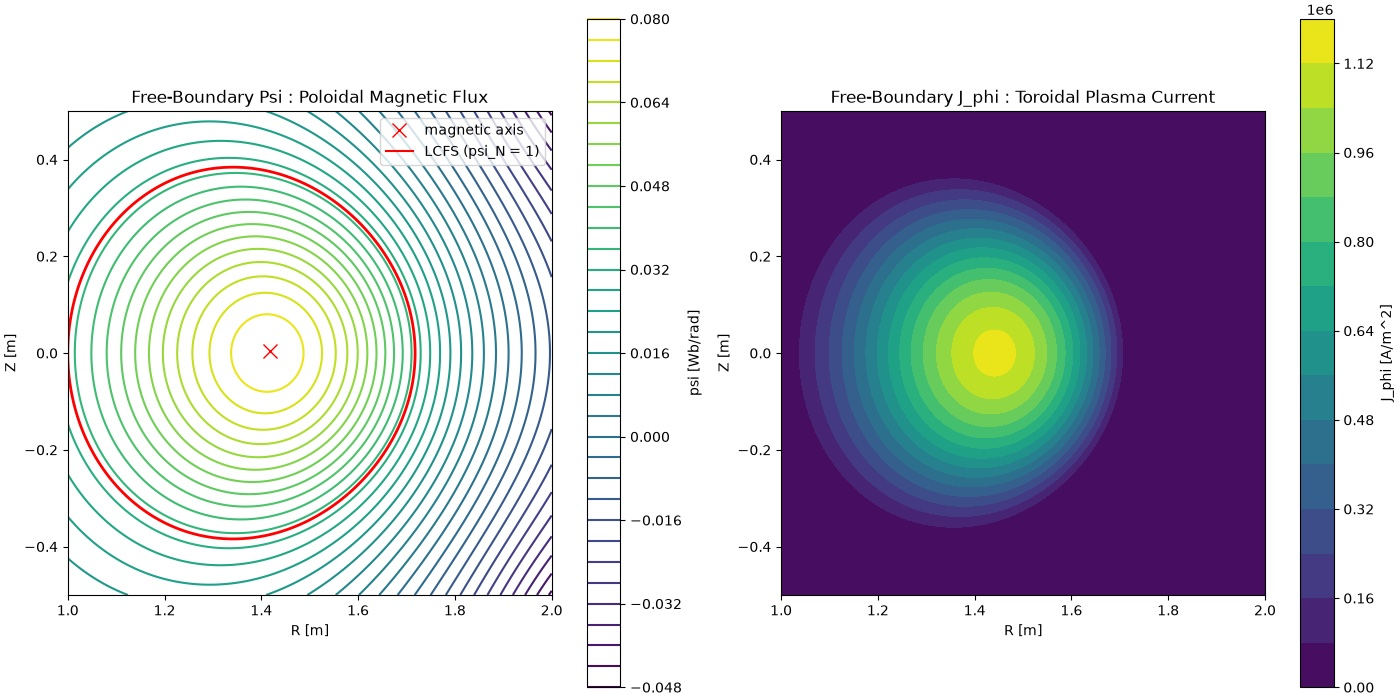
\includegraphics[width=0.9\textwidth]{gs_free_boundary_fixed.jpg}
\caption{Рівновага з вільною межею після ремонту \texttt{Tokamak-GS-solver} (29.09.2026), типовий приклад \texttt{test\_free\_boundary.py}: сітка $128\times128$ у прямокутнику $R\in[1;\,2]$~м, $Z\in[-0{,}5;\,0{,}5]$~м; $\Ip=\SI{200}{кА}$ (множник $\lambda$ підлаштовується під $\Ip$), $\beta_0=1$, $m=n=1$; дві котушки PF по $-\SI{90}{кА}$ у $(2{,}2;\,\pm0{,}7)$~м поза сіткою. Ліворуч --- $\psi$ [Вб/рад], хрестик --- магнітна вісь ($R\approx\SI{1.42}{м}$), червоний контур --- LCFS ($\psiN=1$); праворуч --- $\Jtor$ [А/м$^2$], нуль поза маскою плазми. LCFS торкається внутрішнього краю сітки $R=\SI{1}{м}$: межу плазми тут задає прямокутник розрахункової області, а не X-точка чи лімітер. Власний розрахунок~\cite{ProjGSsolver}.}\label{fig:03-gsfb}
\end{figure}

\begin{figure}[htbp]\centering
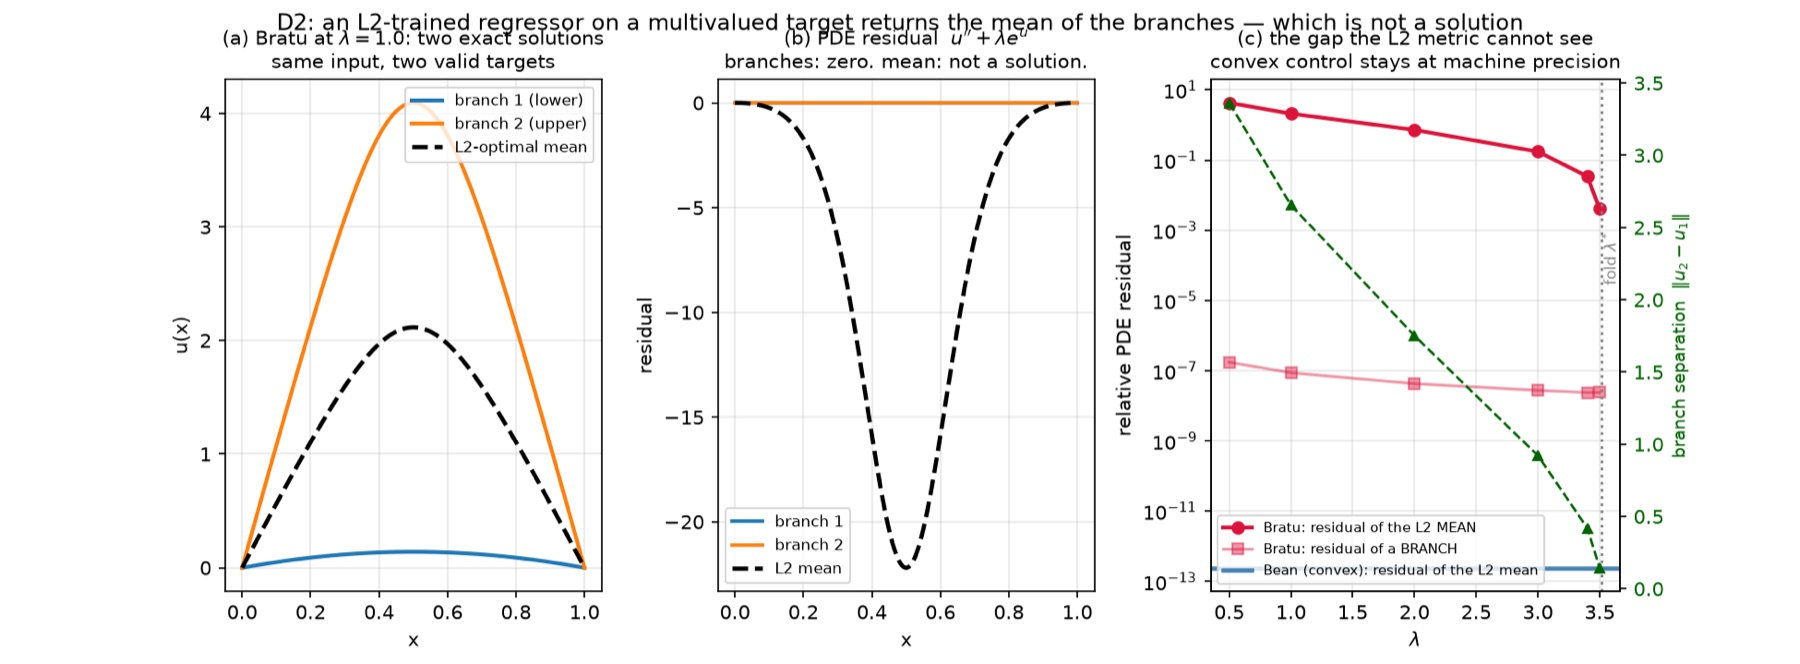
\includegraphics[width=0.85\textwidth]{d2_branch_mean.jpg}
\caption{D2: задача Брату (на рисунку $\lambda\equiv\lambda_{\mathrm{B}}$). (a)~Дві точні гілки при $\lambda_{\mathrm{B}}=1$ і їхнє $L^2$-середнє. (b)~Нев'язка $u''+\lambda_{\mathrm{B}}\ee^u$: для гілок нуль, для середнього мінімум $\approx-22$ у центрі. (c)~Відносна нев'язка середнього і гілки та відстань між гілками залежно від $\lambda_{\mathrm{B}}$; пунктир --- точка складки; контроль Біна --- на рівні машинної точності. Власний розрахунок~\cite{ProjDeepDives}.}\label{fig:03-d2}
\end{figure}

\begin{established}{E21, E24, E4, E5}
\textbf{Джерела~\cite{ProjRegisters}.} E21: розв'язок GS \emph{може бути неєдиним} на реальній геометрії (Ham і Farrell, 2024; Pentland та ін., 2025, MAST-U, дефляційна континуація). E24: критичний стан Біна опуклий і має єдиний розв'язок, а задача плазми з вільною межею неопукла і багатозначна.
\textbf{Власний вимір~\cite{ProjDeepDives} (D2).} Як сурогат механізму взято одновимірну задачу Брату $-u''=\lambda_{\mathrm{B}}\ee^{u}$, $u(0)=u(1)=0$. Нижче точки складки $\lambda_{\mathrm{B}}^*=3{,}513830719$ вона має рівно дві гілки; обчислена $\lambda_{\mathrm{B}}^*$ збігається з літературою до останньої цифри (E5). E4: $L^2$-середнє двох гілок (до нього збігається регресор з $L^2$-втратою) має відносну нев'язку $1{,}22$ проти $6{,}4\cdot10^{-8}$ у гілки; в опуклому контролі (Бін) нев'язка середнього $2{,}5\cdot10^{-13}$.
\textbf{Застереження:} Брату --- \emph{не} GS; перенесення на GS спирається на цитати (рис.~\ref{fig:03-d2}).
\end{established}



\begin{conjecture}{C7}
\textbf{Що стверджує:} Deep Ritz (мінімізація функціонала енергії нейромережею) на неопуклій задачі плазми буде нестабільним відносно seed (обиратиме різні гілки). На опуклій задачі Біна він буде стабільним~\cite{ProjRegisters}. \textbf{Що спростує:} обидві задачі стабільні, тобто неопуклість не виявляється на доступних масштабах. \textbf{Вартість:} близько дня, потрібні обидва розв'язувачі. \textbf{Що зробити:} взяти \texttt{src/examples/deep\_ritznet.py}~\cite{ProjGSsolver} (опуклий пуассонівський функціонал) і замінити функціонал на $\int(\tfrac12u'^2-\lambda_{\mathrm{B}}\ee^u)$. Прогнати 20 seed і класифікувати результати за $\max u$. Увага: функціонал необмежений знизу, а верхня гілка --- сідло, тож «нестабільність» може виявитися розбіжністю, а не вибором іншої гілки; ці випадки треба розрізняти.
\end{conjecture}


\begin{figure}[htbp]\centering
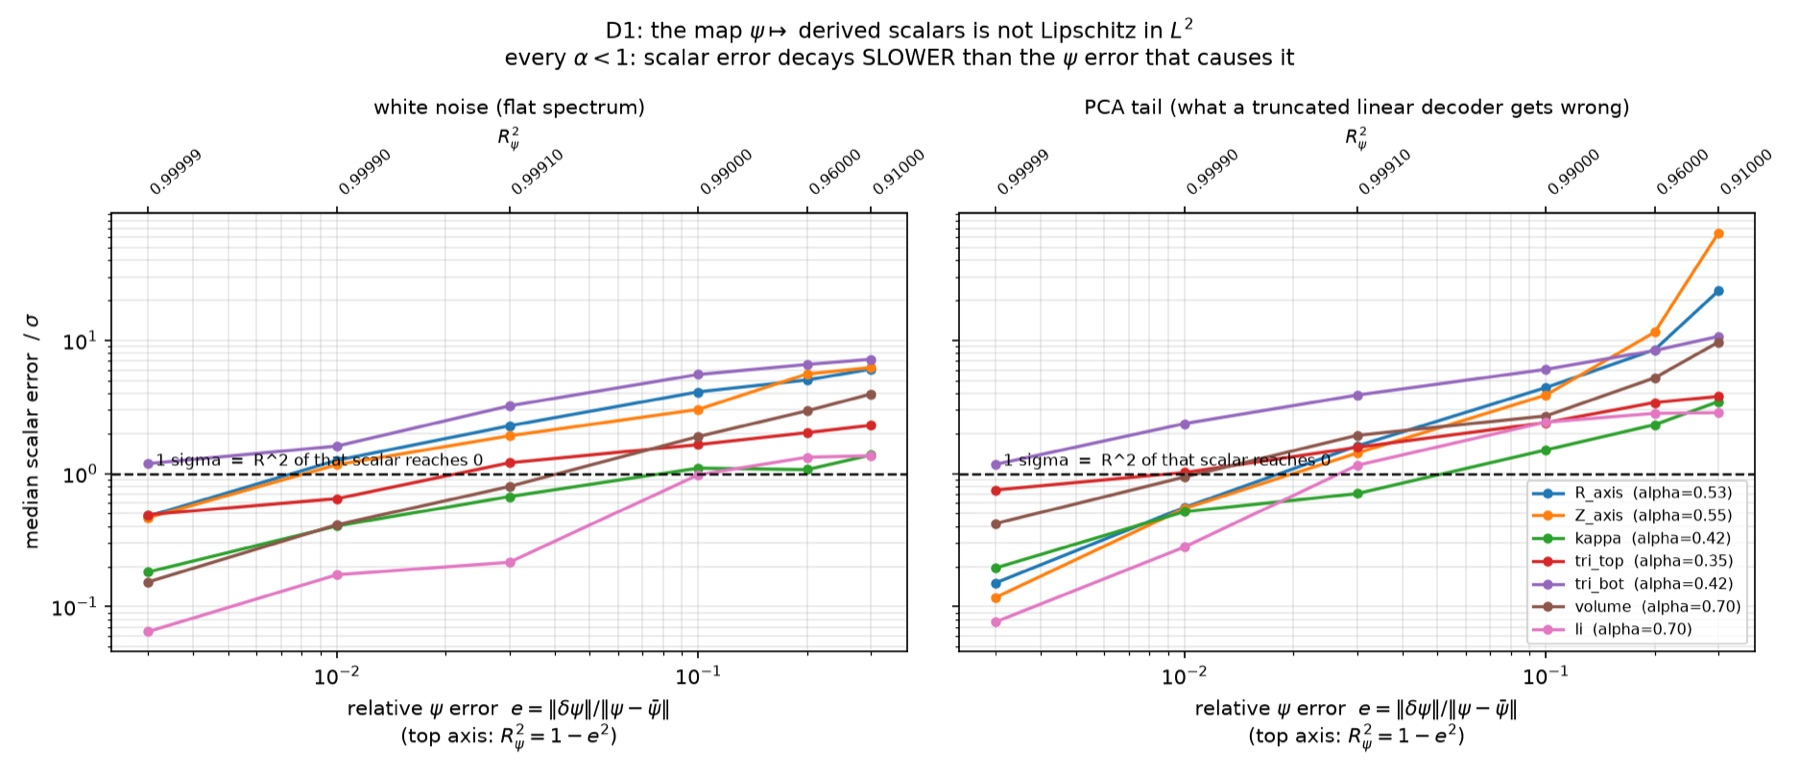
\includegraphics[width=\textwidth]{d1_amplification.jpg}
\caption{D1: медіанна похибка семи скалярів (в одиницях популяційного $\sigma$) залежно від відносної похибки $e=\|\delta\psi\|/\|\psi-\bar\psi\|$, $R^2_\psi=1-e^2$. Ліворуч --- білий шум, праворуч --- хвіст PCA. Усі нахили $a_e<1$. 60 кадрів трьох демо-розрядів DIII-D. Власний розрахунок~\cite{ProjDeepDives}; дані:~\cite{FEC2026}, CC~BY~4.0.}\label{fig:03-d1}
\end{figure}

\begin{established}{E6--E8}
Нев'язку GS можна обчислити з одного лише $\psi$, без поданих $p'$ і $FF'$, бо в структурі EFIT джерело лінійне за коефіцієнтами профілів~\cite{ProjRegisters}:
\[
g(\psi)=\min_{c_i,d_j}\frac{\big\|\GSop\psi-\sum_{i<4}c_iR^2\psiN^{\,i}-\sum_{j<4}d_j\psiN^{\,j}\big\|}{\|\GSop\psi\|}
\]
Норму беруть по пікселях плазми (\texttt{Our try/04-novelty/gs\_residual\_probe.py}). На 12 кадрах DIII-D~\#203702: E6 --- істина (EFIT) $0{,}009$; з 1\,\% шуму $0{,}650$ (у 70 разів більше); з 3\,\% шуму $0{,}921$; E7 --- $g$ інваріантна до масштабу: $\psi\times1{,}05$ дає те саме значення; E8 --- $g$ сліпа до гладких похибок: гаусове згладжування $0{,}010$, PCA-5 $0{,}0093$ (раніше в реєстрі стояло $0{,}016$ без скрипта-джерела; перерахунок 2026-09-29 тими самими функціями дає $0{,}0093$, тож висновок про сліпоту лише посилився). Причина сліпоти: $\GSop$ --- оператор другого порядку, він підсилює високі хвильові числа.
\end{established}


\begin{established}{E1--E3, E14, E36}
Скаляри рівноваги є диференціальними функціоналами $\psi$~\cite{ProjRegisters,ProjDeepDives}: вісь --- критична точка $\grad\psi=0$, форма (витягнутість, трикутність, об'єм) --- контур крізь сідло, $\li$ --- інтеграл від $|\grad\psi|^2$. E1: відображення $\psi\to$ скаляри не ліпшицеве в $L^2$: похибка скаляра зростає як $e^{a_e}$ з $a_e\in[0{,}35;\,0{,}70]$ (у реєстрі~--- $\alpha$; рис.~\ref{fig:03-d1}). Похибка $R_{\mathrm{ax}}$ сягає $1\sigma$ вже при $R^2_\psi=0{,}99993$, а при $R^2_\psi=0{,}99$ становить 3,4~см. Це виміряно для \emph{білого} (повузлового) шуму; для гладкого збурення $a_e\approx0{,}69$--$1{,}08$ (уточнення 2026-09-30). E2: на трьох демо-розрядах показники утворюють три кластери: $0{,}53$--$0{,}55$, $0{,}35$--$0{,}42$ і $0{,}70$; на ширшій вибірці їх немає (R10). E3: хвіст PCA шкодить більше, ніж білий шум тієї самої енергії: для $Z_{\mathrm{ax}}$ $64{,}4\sigma$ проти $6{,}3\sigma$ при $e=0{,}30$. E14 (синтетичний тест): зсув осі під шумом пропорційний $1/\sqrt{\lambda_H}$, де $\lambda_H$ --- кривизна (власне значення гесіана $\psi$) в O-точці. Добуток $|\Delta x|\sqrt{\lambda_H}$ сталий з точністю $\pm7\,\%$ на 16-кратному діапазоні $\lambda_H$; тест відновлено 2026-09-30 (для $R_{\mathrm{ax}}$ $\pm5{,}6\,\%$, \texttt{c1/e14\_curvature.py}). \textbf{E36:} скорер шукає вісь як максимум на вузлах із параболічним уточненням, тому для шуму амплітуди $\eta$ у вузлі $a_e=1$, поки $\eta<\eta^{*}=\lambda_H h^2/2$, і $a_e\approx0{,}4$--$0{,}5$ вище, де дискретний максимум стрибає ($h$ --- крок сітки).
\end{established}
\begin{refuted}{R6}
«$a_e=\tfrac12$ --- універсальний закон» для положення критичної точки (осі). Спростовано: показник залежить від кривизни ($0{,}687$ при $\lambda_H=1$ і $0{,}841$ при $\lambda_H=4$)~\cite{ProjRegisters}. Причину пояснює E36: у фіксованому вікні $\eta$ більша кривизна означає більшу частку лінійного режиму.
\end{refuted}

\begin{refuted}{R10 (була гіпотеза C1)}
«Три кластери E2 відповідають трьом механізмам --- положенню екстремуму, контуру крізь сідло та інтегралу». Критерії записали до перевірки. Розбиття стабільне лише на трьох демо-розрядах (96,7\,\% бутстрепу по розрядах); на 28 розрядах DIII-D --- 0\,\% ($\li$: $a_e$ з $0{,}70$ падає до $0{,}47$), на MAST --- 3,3\,\%, на 12 однонульових рівновагах Серфона--Фрайдберга~\cite{Cerfon2010} --- 0,3\,\%~\cite{ProjRegisters,ProjGuide}. Урок: кластер, побачений на трьох розрядах, --- ще не закон.
\end{refuted}

\begin{conjecture}{C3}
Кривизна $\lambda_H$ з E14 корисна для стратифікації тестової вибірки. \textbf{Спростує:} вузький розподіл $\lambda_H$ по корпусу. \textbf{Стан:} на 28 розрядах DIII-D $\lambda_H\in[0{,}13;\,3{,}6]$ --- розподіл широкий, але $a_e$ осі між терцилями $\lambda_H$ змінюється слабко~\cite{ProjRegisters}. \textbf{Що зробити:} стратифікувати за $\lambda_H$ залишки справжнього бейзлайну PCA+Ridge (код --- \texttt{Our try/03-deep-dives/D1-psi-to-scalars/c1/real\_sweep.py}). Дані --- Fusion Equilibrium Challenge~\cite{FEC2026}.
\end{conjecture}

\paragraph{Відкриті питання~\cite{ProjRegisters}.} Крім \textbf{Q2} (п.~\ref{sec:03-recon}), \textbf{Q3}: чи трапляється неєдиність GS (E21) у робочих режимах (від цього залежить, чи D2 реальна).

\subsection*{Контрольні запитання}
\begin{enumerate}
\item Виведіть \eqref{eq:03-surfaces} з \eqref{eq:03-force}. Чому лінії поля й струму лежать на поверхнях $p=\text{const}$?
\item Як переписати формули Merlo і Ward для нашого $\psi$? Чи змінюється при цьому $\psiN$?
\item Навіщо функція Гріна в задачі з вільною межею? Що забезпечує умова $\int g>I$?
\item Чому магнітні виміри кругової плазми дають лише $\Lambda$? Як це пов'язано з виродженням?
\item Чому $L^2$-середнє гілок не є розв'язком? До чого сліпа GS-нев'язка?
\end{enumerate}

\subsection*{Задачі}
\begin{enumerate}
\item \emph{Вертикальне поле RFX-mod.} Візьміть $R_0=\SI{2}{м}$, $r_a=\SI{0.459}{м}$ (радіус першої стінки), $\Ip=\SI{150}{кА}$ (порядок величини з рис.~3.2 у~\cite{Merlo2011}; перевірте: за $\Bzero=\SI{0.6}{\tesla}$ маємо $q(a)\approx2{,}1$). (а)~Обчисліть $B_{v,\mathrm{eq}}$ \eqref{eq:03-Bv} для двох параметризацій розряду \#29648 (п.~\ref{sec:03-param}); наскільки у відсотках відрізняються результати? (б)~Оцініть $\Delta_{\mathrm{S}}(0)$ за формулою з рамки для $\betap=0{,}26$, $\li=1{,}00$.
\item \emph{Брату.} Розв'язок: $u=-2\ln\bigl[\cosh\bigl(\theta(x-\tfrac12)/2\bigr)/\cosh(\theta/4)\bigr]$, $\lambda_{\mathrm{B}}=\theta^2/\bigl[2\cosh^2(\theta/4)\bigr]$.
  (а)~Знайдіть $\lambda_{\mathrm{B}}^*$. (б)~Для $\lambda_{\mathrm{B}}=1$ знайдіть $u_{\max}$ обох гілок. (в)~Обчисліть нев'язку $L^2$-середнього в точці $x=\tfrac12$ і порівняйте з рис.~\ref{fig:03-d2}(b).
\item \emph{Інваріантність E7.} Покажіть, що коли $\psi$ розв'язує \eqref{eq:03-GS} з $(p',FF')$, то $c\psi$ розв'язує його з перемасштабованими профілями. Чому \emph{незалежний} піксельний шум це руйнує?
\end{enumerate}

\chapter{Геометричні ефекти}\label{ch:geometry}

Рівновага (розд.~\ref{ch:equilibrium}) дає функцію $\psi(R,Z)$. У цьому розділі з неї будуємо координати, в яких записують рівняння переносу й потоків (розд.~\ref{ch:transport}, \ref{ch:flows}), розбираємо, як форма перерізу впливає на стійкість, і закінчуємо топологією $\psi$: критичними точками, сепаратрисою та дослідницьким треком проєкту.

\section{Системи координат і метрика}\label{sec:04-coords}

\begin{outofcorpus}[потокові координати, кут прямих силових ліній, усереднення]
Візьмемо $(\psi,\theta,\tor)$, де $\theta$ --- будь-який полоїдальний кут на поверхні $\psi=\text{const}$, і якобіан $\mathcal{J}^{-1}=\grad\psi\times\grad\theta\cdot\grad\tor$ (об'єм $\dd V=\mathcal{J}\,\dd\psi\,\dd\theta\,\dd\tor$). З $\Bvec=\grad\psi\times\grad\tor+F\grad\tor$ \eqref{eq:03-B} маємо $\Bvec\cdot\grad\tor=F/R^2$ і $\Bvec\cdot\grad\theta=-1/\mathcal{J}$. Тому лінія поля має $\dd\theta/\dd\tor=-R^2/(F\mathcal{J})$, а запас стійкості та кут прямих силових ліній (straight-field-line angle)
\begin{equation}\label{eq:04-q}
q(\psi)=\frac{1}{2\pi}\oint\frac{F|\mathcal{J}|}{R^2}\,\dd\theta=\frac{\dd\psit}{\dd\psi},\qquad
\thetastar=\frac{1}{q}\int_0^{\theta}\frac{F|\mathcal{J}|}{R^2}\,\dd\theta',\qquad \frac{\dd\thetastar}{\dd\tor}=\frac1q
\end{equation}
(знак залежить від орієнтації кутів і напрямків $\Ip$, $\Btor$). Друга рівність для $q$ випливає з того, що тороїдальний потік на радіан $\psit=\Psit/2\pi=\frac{1}{2\pi}\int\Btor\,\dd A$ ($\Psit$~--- повний потік), а елемент площі перерізу $\dd A=|\mathcal{J}|R^{-1}\dd\psi\,\dd\theta$. У змінних $(\thetastar,\tor)$ силові лінії --- прямі; саме ця пара разом з $\psit$ утворює канонічні змінні з розд.~\ref{ch:particles}.

\emph{Усереднення по магнітній поверхні}: $\fsa{f}=\oint f\,|\mathcal{J}|\,\dd\theta\big/\oint|\mathcal{J}|\,\dd\theta$, $V'=\dd V/\dd\psi=2\pi\oint|\mathcal{J}|\,\dd\theta$. Основні тотожності для однозначних осесиметричних $f$ (або з усередненням і по $\tor$) і векторних полів $\vect{A}$:
\begin{equation}\label{eq:04-fsa}
\fsa{\Bvec\cdot\grad f}=0,\qquad \fsa{\grad\cdot\vect{A}}=\frac{1}{V'}\frac{\dd}{\dd\psi}\Big(V'\fsa{\vect{A}\cdot\grad\psi}\Big).
\end{equation}
Перша випливає з $\Bvec\cdot\grad f=-\mathcal{J}^{-1}\pa_\theta f+(F/R^2)\pa_\tor f$ (інтеграл від повної похідної по замкненому контуру дорівнює нулю). Друга --- з формули дивергенції в координатах. Саме \eqref{eq:04-fsa} прибирає з рівнянь переносу паралельну динаміку й залишає одновимірні рівняння за $\psi$ (розд.~\ref{ch:transport}).
\end{outofcorpus}

\paragraph{Координати Бузера.} Це координати прямих силових ліній, у яких ще й коваріантні компоненти $B_\theta$, $B_\tor$ є функціями потоку (стандартне означення, поза корпусом). Тищенко~\cite[с.~25]{Tyshchenko2021} записує рівняння альфвенівських хвиль у координатах Бузера $(\Psit,\theta,\tor)$ з радіальною змінною~--- тороїдальним потоком і поздовжнім оператором $q^{-1}\pa_\theta+\pa_\tor$ (у джерелі полоїдальний кут позначено іншою літерою, а в підписі до (1.4) назви кутів переставлено; з множника $\exp(im\theta-in\tor)$ видно, що $\theta$ --- полоїдальний). Метрика в параксіальному наближенні~\cite[с.~26]{Tyshchenko2021}: $B=\bar B[1+\epsilon_B\cos(m_c\theta-n_cN\tor)]$ і аналогічно для $g^{ij}$, причому $g^{11},g^{22}\propto\delta_\kappa=(\kappa+\kappa^{-1})/2$. «Параметри зачеплення» $\epsilon_B$, $\epsilon_g$ зв'язують гармоніки $m$ і $m+m_c$: $m_c=1$ відповідає тороїдальності, $m_c=2$ --- витягнутості; у токамаку $n_c=0$. Отже, форма перерізу прямо входить у спектр хвиль через метрику.

\paragraph{MSCS Seto.} Для 2D-моделі ядра й периферії Seto і Fukuyama~\cite[с.~2]{Seto2014} беруть систему координат магнітної поверхні (MSCS). У наших позначеннях це $(\rho_{\mathrm{M}},\theta_{\mathrm{M}},\tor)$ (в оригіналі кути позначено іншими літерами). Радіальна мітка $\rho_{\mathrm{M}}$ будується з тороїдального потоку; полоїдальний кут $\theta_{\mathrm{M}}$ --- нормована довжина проєкції силової лінії на площину $\tor=\text{const}$; $\tor$ --- геометричний тороїдальний кут, тому $\vect{e}_\tor=R^2\grad\tor$ ортогональний до двох інших напрямків. Поле $\Bvec=\grad\tor\times\grad\psi+I\grad\tor$ (наше $\psi$ з точністю до знака і нормування, $I\equiv F$), $q=\dd\psit/\dd\psi$ у згоді з \eqref{eq:04-q}. Оскільки кути визначено незалежно від потокових функцій, MSCS «не потокова» і, на відміну від $(\psi,\thetastar,\tor)$, придатна й за сепаратрисою, де $q\to\infty$.

\paragraph{Координати GTC.} Гірокінетичний код GTC~\cite[с.~6--7]{Wang2006} використовує потокові координати прямих силових ліній з геометричним $\tor$ і радіусом $r=\sqrt{\Psit/\Psi_{\mathrm{t,b}}}$ ($\Psi_{\mathrm{t,b}}$ --- на межі плазми). Масштаб дрейфової турбулентності $\propto\rho_{\mathrm i}\propto\sqrt{T_{\mathrm i}}$, а в NSTX $T_{\mathrm i}$ падає від $\sim$\,кеВ у центрі до $\sim\SI{10}{еВ}$ біля сепаратриси~\cite[с.~6]{Wang2006}. Тому сітку роблять рівномірною за
\begin{equation}\label{eq:04-gtc}
\frac{\dd\rho_{\mathrm{G}}}{\dd r}=\sqrt{\frac{T_{\mathrm c}}{T_{\mathrm i}(r)}},\qquad \Delta r\sim\sqrt{T_{\mathrm i}(r)/T_{\mathrm c}},
\end{equation}
де $T_{\mathrm c}$ --- температура в опорній точці~\cite[с.~7, (1)]{Wang2006}. Полоїдальний крок $\Delta\theta(r)$ сталий на поверхні і добирається так, щоб дуга біля екватора була $\sim\rho_{\mathrm i}$; тривимірна сітка йде вздовж наближених ліній $\bar q(r)\theta-\tor=\text{const}$.

\section{Форма перерізу і вертикальна стійкість}\label{sec:04-shape}

\begin{outofcorpus}[параметри форми]
За крайніми точками LCFS: $R_{\mathrm{geo}}=(R_{\max}+R_{\min})/2$, $a=(R_{\max}-R_{\min})/2$, аспектне відношення $A=R_{\mathrm{geo}}/a$, витягнутість $\kappa=(Z_{\max}-Z_{\min})/2a$, верхня і нижня трикутності $\dup=(R_{\mathrm{geo}}-R_{Z_{\max}})/a$, $\dlo=(R_{\mathrm{geo}}-R_{Z_{\min}})/a$, де $R_{Z_{\max}}$ --- радіус найвищої точки. Витягнутість дає більший струм за того самого $q$, але потребує зовнішнього поля з від'ємним індексом спаду $n_{\mathrm d}<0$, що робить плазму вертикально нестійкою.
\end{outofcorpus}

\paragraph{Індекс спаду поля.} Для зовнішнього вертикального поля $n_{\mathrm d}=-(R/\BZ)\,\pa\BZ/\pa R$. Кругова плазма вертикально стійка при $n_{\mathrm d}>0$ і горизонтально стійка при $n_{\mathrm d}<3/2$~\cite[с.~76]{Merlo2011}. У double-null (DN) конфігурації RFX-mod котушки F8 збільшують об'єм і трикутність, витягуючи плазму назовні, і на різних ділянках екватора порушено \emph{обидві} умови. Лінеаризована модель з резистивними пасивними структурами (ще без сідлових котушок) має дві нестійкі моди, причому горизонтальна домінує: $\tau_{\mathrm{hor}}=\SI{51.12}{мс}$, $\tau_{\mathrm{vert}}=\SI{60.72}{мс}$~\cite[с.~75--76]{Merlo2011}. Активну стабілізацію розглянуто в розд.~\ref{ch:stability}.

\begin{corpusexample}[пасивна стабілізація і деформованість~\cite{Ward1992}]
NOVA-W розраховує вертикальну моду з двома симетричними провідними пластинами (кожна $\approx1/8$ периметра стінки, опір як в алюмінію товщиною \SI{1}{см}); кут $|\Theta_{\mathrm{pl}}|$ відраховують від зовнішнього екватора (с.~11).
\begin{itemize}
\item Еліпс $A=100$, $\kappa=2$: оптимум $|\Theta_{\mathrm{pl}}|=\pi/2$ (над і під плазмою), інкремент лише $\approx3{,}5$ раза більший, ніж з повною стінкою (с.~11--12).
\item Еліпс $A=4{,}5$ з витягнутістю ARIES-I і нульовою трикутністю: оптимум зсувається назовні, $|\Theta_{\mathrm{pl}}|\approx0{,}448\pi$ (тороїдальність, с.~15).
\item CIT ($R_0=\SI{2.182}{м}$, $a=\SI{0.660}{м}$, $\kappa_{95}=1{,}996$, $\delta_{95}=0{,}258$, с.~17): $|\Theta_{\mathrm{pl}}|\approx0{,}403\pi$; ідеальна стійкість лише при $\pi/4\lesssim|\Theta_{\mathrm{pl}}|\le\pi/2$ (с.~18--19).
\item ARIES-I ($\kappa=1{,}61$, $\delta=0{,}43$): $|\Theta_{\mathrm{pl}}|\approx0{,}394\pi$, хоча $A$ більше, ніж у CIT. Трикутність зсуває оптимум назовні сильніше, ніж тороїдальність (с.~19).
\end{itemize}
Причина --- деформованість: плазма «обтікає» пластини, гармоніки $m=2,3$ перебудовуються і зменшують стабілізуючі вихрові струми. Рівноваги в~\cite{Ward1992} штучно дестабілізовано, тож числа ілюструють тенденцію, а не проєкт.
\end{corpusexample}

Профіль струму впливає на форму через $\li$ і $\Lambda$ \eqref{eq:03-Bv}. За стандартною теорією (поза корпусом), що більша $\li$, то менше струму на периферії і то важче стабілізувати витягнутий переріз (розд.~\ref{ch:stability}).

\section{Конфігурації}\label{sec:04-configs}

\textbf{Лімітер і дивертор.} LCFS або торкається лімітера, або проходить крізь X-точку, і тоді межа --- сепаратриса~\cite[с.~30]{Merlo2011}. Дивертор відводить найбільші теплові навантаження в точки перетину сепаратриси зі стінкою, керовані положенням X-точки (розд.~\ref{ch:wall}). \textbf{Double-null} (дві X-точки): у RFX-mod розряд \#29746 відтворено з $\li=0{,}95$, $\betap=0{,}29$~\cite[с.~38]{Merlo2011}; реконструкція межі підтверджує, що DN було досягнуто, але згодом конфігурація деградувала до лімітерної, бо регулятора форми не було~\cite[с.~54]{Merlo2011}. \textbf{Від'ємна трикутність}: AUG \#36026 --- перша спроба на AUG, переважно через верхню трикутність. Fenix добре відтворює розряд до \SI{3}{с}, але в H-моді симуляція дає плазму, обмежену \emph{зовнішнім} лімітером, а реконструкція --- \emph{внутрішнім}; причина невідома~\cite[с.~7--8]{Fable2022}. \textbf{Сферичний токамак} NSTX: $A\approx1{,}2$ (модельні $R_0$, $a$ з табл.~\ref{tab:01-devices}). TSC+DCON прогнозують, що при нагріванні NBI до \SI{5}{МВт} енергетично досяжне $\beta>15\,\%$, але балонна нестійкість починається при $\beta\approx12\,\%$ через малий шир біля $q=1$ і пікований тиск~\cite[с.~5]{Jardin2000}. \textbf{Симетрія і власне обертання.} Напрям спонтанного обертання визначає симетрія поля (токамак проти геліотрона)~\cite[с.~6--7]{Ida2001}; див. п.~\ref{sec:06-intrinsic}.

\textbf{Гофрування TF-поля} --- порушення осесиметрії з періодом $2\pi/N_{\mathrm{TF}}$ --- розглянуто в п.~\ref{sec:02-ripple}. Усе нижче стосується осесиметричного $\psi$.

\section{Топологія $\psi(R,Z)$: O- і X-точки, сепаратриса}\label{sec:04-topology}

\begin{figure}[htbp]\centering
\begin{minipage}[c]{0.38\textwidth}\centering
\begin{tikzpicture}[scale=0.62,>=Stealth]
 \foreach \s in {0.35,0.6,0.85}
   \draw[gray] (0.08,0.15) ellipse ({1.75*\s} and {2.5*\s});
 \draw[thick,blue!70!black] (0,-2.6) .. controls (1.3,-1.7) and (2.0,-0.6) .. (2.0,0.4)
   .. controls (2.0,2.2) and (1.0,2.9) .. (0,2.9) .. controls (-1.0,2.9) and (-2.0,2.2) .. (-2.0,0.4)
   .. controls (-2.0,-0.6) and (-1.3,-1.7) .. (0,-2.6);
 \draw[thick,blue!70!black] (0,-2.6) -- (0.75,-3.4) (0,-2.6) -- (-0.75,-3.4);
 \draw[dashed,gray] (-1.3,-3.4) .. controls (-2.6,-1.5) and (-2.6,3.4) .. (0,3.45)
   .. controls (2.6,3.4) and (2.6,-1.5) .. (1.3,-3.4);
 \draw[very thick] (-1.6,-3.4) -- (1.6,-3.4);
 \fill (0.08,0.15) circle (2.5pt) node[right,font=\scriptsize] {O ($+1$)};
 \fill[red!70!black] (0,-2.6) circle (2.5pt) node[right=2pt,font=\scriptsize] {X ($-1$)};
 \node[font=\scriptsize,blue!70!black] at (2.05,2.6) {LCFS};
 \node[font=\scriptsize,gray] at (-2.35,2.95) {SOL};
\end{tikzpicture}
\end{minipage}\hfill
\begin{minipage}[c]{0.6\textwidth}\centering
\begin{tikzpicture}\node[inner sep=0] (im) {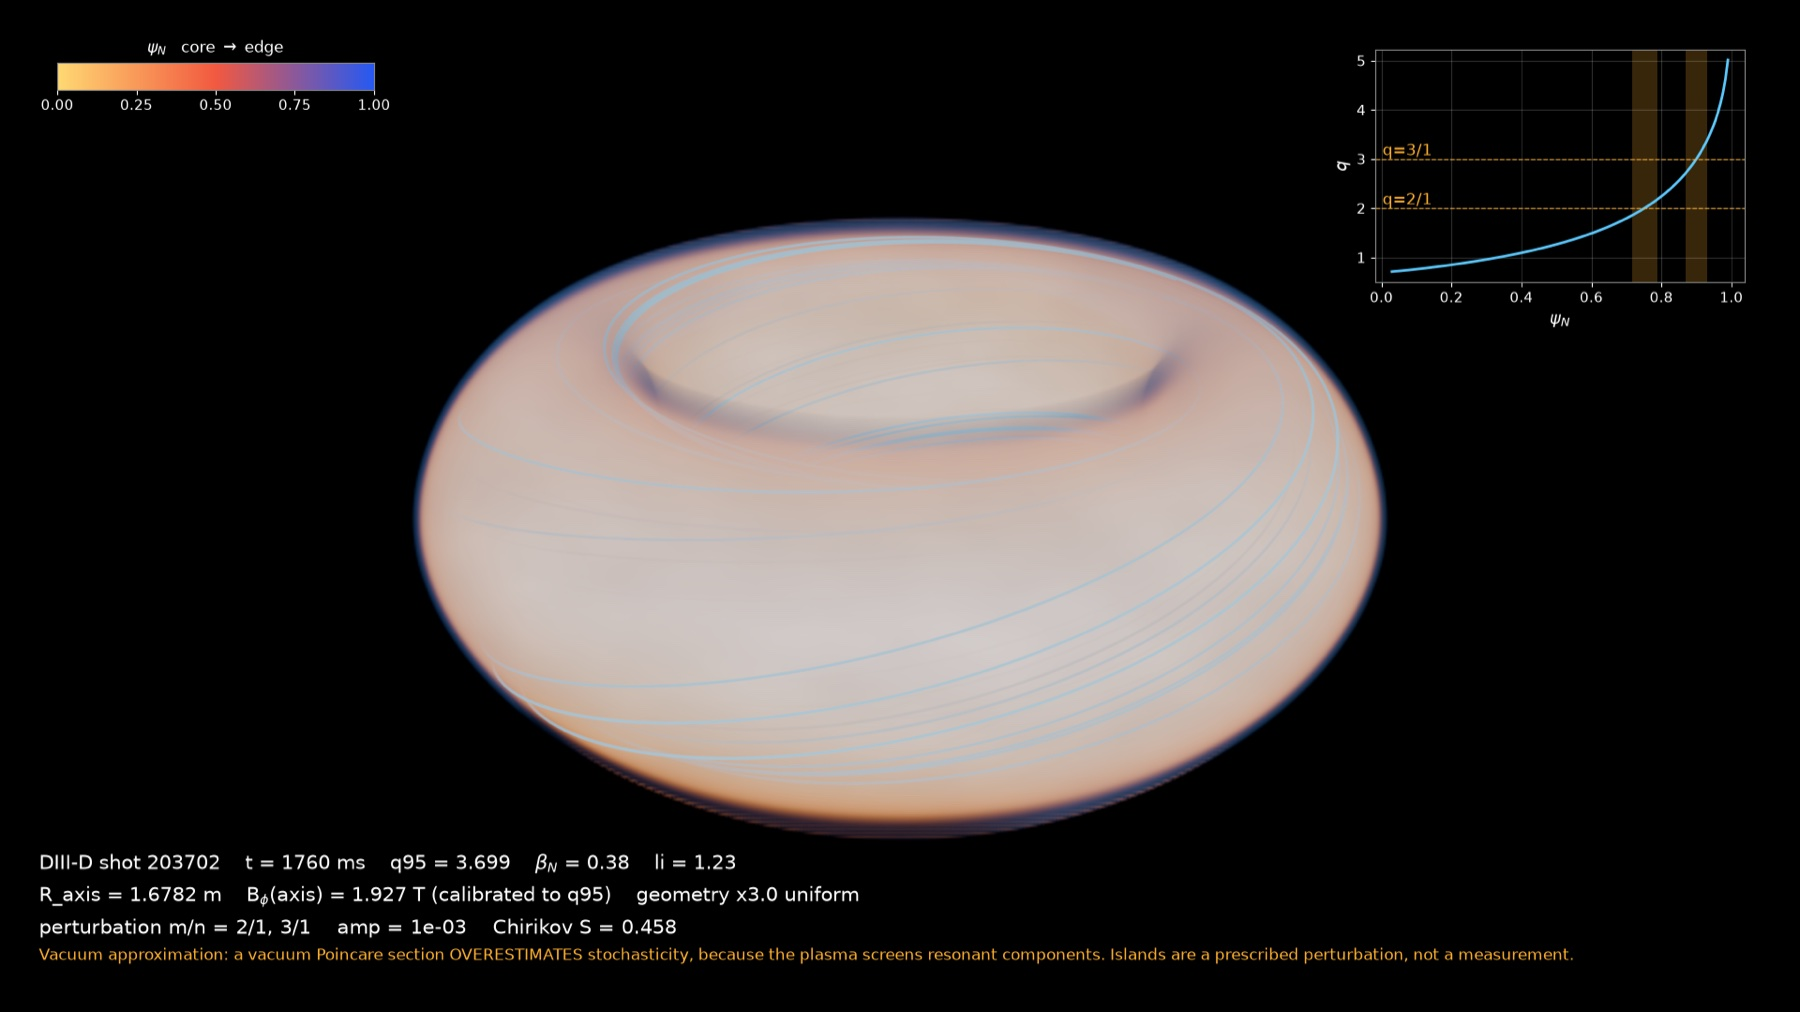
\includegraphics[width=\textwidth,trim=405 168 405 205,clip]{viz_plasma.jpg}};
 \fill[black] ($(im.north east)+(-7mm,0)$) rectangle ($(im.north east)+(0,-11mm)$);\end{tikzpicture}
\end{minipage}
\caption{Ліворуч: схема критичних точок $\psi$ в однонульовій конфігурації (у дужках --- індекс Пуанкаре--Хопфа), сепаратриса (LCFS) з двома ногами до дивертора, відкриті лінії SOL. Праворуч: об'ємний рендер плазми DIII-D \#203702, $t=\SI{1760}{мс}$, $\qnf=3{,}70$ (фрагмент рис. \texttt{viz\_plasma}); колір --- $\psiN$ від осі до краю, блакитні лінії --- силові лінії на магнітних поверхнях. Власний розрахунок~\cite{ProjViz}; дані рівноваги: Fusion Equilibrium Challenge (Sophelio / General Atomics), CC BY 4.0.}\label{fig:04-topo}
\end{figure}

\begin{outofcorpus}[критичні точки, індекс, теорія Морса]
Критична точка $\grad\psi=0$ --- це нуль $\Bpol=|\grad\psi|/R$. Гесіан $\mathsf{H}_\psi$ класифікує її: $\det\mathsf{H}_\psi>0$ --- еліптична O-точка (магнітна вісь або центр острова), індекс $+1$; $\det\mathsf{H}_\psi<0$ --- гіперболічна X-точка, індекс $-1$. Індекс дорівнює числу обертів вектора $\grad\psi$ уздовж малого контуру навколо точки. \emph{Теорема Пуанкаре--Хопфа}: якщо $\grad\psi$ трансверсальний до межі області $D$, сума індексів усередині дорівнює ейлеровій характеристиці $\chi_{\mathrm{E}}(D)$; для диска $\chi_{\mathrm{E}}=1$. \emph{Теорія Морса}: топологія підрівневої множини $\{\psiN\le t\}$ змінюється лише при проходженні критичних значень; мінімум додає компоненту ($\chi_{\mathrm{E}}\to\chi_{\mathrm{E}}+1$), сідло --- з'єднує дві компоненти або додає дірку ($\chi_{\mathrm{E}}\to\chi_{\mathrm{E}}-1$). Для вкладених поверхонь (одна O-точка, всередині LCFS сідел немає) $\chi_{\mathrm{E}}(\{\psiN\le t\})=1$ при всіх $t<1$. Сепаратриса --- рівень $\psi$, що проходить через X-точку; у диверторній плазмі вона і є LCFS. Шум, який народжує пару O--X, не змінює суми індексів.
\end{outofcorpus}

Критичні точки --- це саме те, що рахують скаляри рівноваги: положення осі, форма межі через сідло (розд.~\ref{ch:equilibrium}, E1--E3). Проєкт перевірив, чи дає скелет критичних точок (рис.~\ref{fig:04-topo}) незалежний критерій якості передбаченого $\psi$~\cite{ProjRegisters,FEC2026}. Індекс рахують як число обертів $\grad\psi$ навколо 8 сусідів кожного пікселя. Сусідні пікселі з ненульовим індексом об'єднують у компоненту, і для неї рахують число обертів по периметру обмежувального прямокутника (одна справжня точка займає блок $2\times2$). Область --- внутрішність LCFS, ерозована на 2 пікселі, щоб X-точки не потрапили в неї.

\begin{established}{E9--E11}
\cite{ProjRegisters}; \texttt{topology\_probe.py}, DIII-D \#203702, 8 кадрів, гаусів шум $\varepsilon\cdot\mathrm{std}(\psi)$ (перевірено повторним прогоном):
\begin{center}\small
\begin{tabular}{@{}lcccccc@{}}\toprule
$\varepsilon$ & 0 & 0,001 & 0,003 & 0,01 & 0,03 & 0,10\\\midrule
$R^2_\psi$ & 1 & 1 & 0,99999 & 0,99993 & 0,99935 & 0,99278\\
O / X (медіана) & 1 / 0 & 1 / 0 & 1 / 0 & 1 / 0 & 1 / 0 & 10,5 / 11,0\\
сума індексів & $+1$ & $+1$ & $+1$ & $+1$ & $+1$ & $+1{,}5$\\\bottomrule
\end{tabular}
\end{center}
E9: істина має рівно одну O-точку і жодного сідла. E10: скелет стійкий до 3\,\% шуму, а на 10\,\% з'являється 20,5 зайвих точок. E11: сума індексів при цьому лишається близькою до $+1$, бо зайві точки народжуються парами O--X. Тому інформативна лише \emph{кількість} точок, а не сума. Кожна зайва O-точка --- острів, якого немає.
\end{established}

\begin{established}{E12--E13}
\texttt{topology\_ec\_curve.py}: на істині $\chi_{\mathrm{E}}(\{\psi\le t\})=1$ на всіх 40 рівнях усередині LCFS (кожна підрівнева множина --- диск; еталон без налаштування). Крива $\chi_{\mathrm{E}}(t)$ менш чутлива, ніж лічильник: при 3\,\% шуму відхилення $\overline{|\Delta\chi_{\mathrm{E}}|}=0{,}14$, а медіана кількості точок 1,5 («лічильник спрацював»; у \texttt{topology\_ec\_curve.py} інша реалізація шуму; на 3\,\% лічильник на межі спрацювання: 1 або 1,5); при 10\,\% --- 4,1 і 17. За Морсом крива є інтегралом від лічильника~\cite{ProjRegisters}.
\end{established}

\begin{refuted}{R5}
«Крива $\chi_{\mathrm{E}}(t)$ краща за лічильник критичних точок». Ні: вона менш чутлива (E13), бо за Морсом лише підсумовує ту саму інформацію; пара мінімум--сідло, чиї критичні значення лежать між двома сусідніми рівнями $t$, не змінює $\chi_{\mathrm{E}}$ на жодному рівні (внески $+1$ і $-1$ скорочуються)~\cite{ProjRegisters}. Роль кривої --- бінарний шлюз допустимості, а не градуйована метрика.
\end{refuted}

\begin{established}{E15--E16}
\texttt{h5\_transfer\_topology.py}: DIII-D і MAST обидві мають скелет 1O/0X із сумою $+1$ (8/8 кадрів кожна), попри протилежні конвенції знака (\texttt{AXIS\_SIGN}: DIII-D $-1$, MAST $+1$), різні сітки й геометрію --- критерій машинно-незалежний (E15). Проєкція MAST на PCA-базис DIII-D з $k=5$, 10, 20, 50 компонентами дає $R^2_\psi=0{,}66$, $0{,}88$, $0{,}93$, $0{,}96$, але скелет лишається 1O/0X (E16)~\cite{ProjRegisters}. Уточнення 2026-09-29: при $k=50$ позначка «1O/0X» у таблиці скрипта --- це медіана $N_X=0{,}5$, округлена до цілого; у 4 із 8 кадрів є внутрішня X-точка. Твердження E16 для $k=5$ це не зачіпає.
\end{established}

\begin{refuted}{R7}
Гіпотеза H5: «провал перенесення DIII-D$\to$MAST має топологічну складову». Спростовано E16: навіть при $R^2_\psi=0{,}66$ топологія ціла. Провал кількісний, а не топологічний~\cite{ProjRegisters}.
\end{refuted}

\begin{refuted}{R9 (була гіпотеза C8)}
\textbf{Було:} збої вилучення LCFS при перенесенні (3/8 кадрів при $k=5$ і 2/8 при $k=20$) --- систематичний сигнал. \textbf{Спростовано 2026-09-29:} усі збої припадають на кадри, де підбір знака обрав $-1$. Функція \texttt{skeleton()} викликала \texttt{extract\_lcfs} без \texttt{axis\_sign}, і оцінювач переходив до резервного варіанта «перший успішний». Якщо повернути реконструкції знак MAST, збоїв немає за жодного $k$. Отже, це артефакт знака~$\psi$, а не властивість перенесення. Скрипт перевірки: \texttt{Our try/04-novelty/c8\_sign\_check.py}~\cite{ProjRegisters}.
\end{refuted}

\begin{practicum}[скелет критичних точок]
Дані: 6 демо-розрядів (3 DIII-D, 3 MAST, 67~МБ) уже лежать у \texttt{fusion equilibrium challenge/starter/parquet\_data/}; окремо їх можна завантажити з GitHub starter kit (Git LFS). Середовище --- \texttt{starter/.venv} (системний \texttt{python3} без \texttt{numpy} не підійде). З теки \texttt{Our try/04-novelty}:\\
\texttt{PY="../../fusion equilibrium challenge/starter/.venv/bin/python"}\\
\texttt{"\$PY" topology\_probe.py; "\$PY" topology\_ec\_curve.py; "\$PY" h5\_transfer\_topology.py}\\
Кожен скрипт працює $\approx1$~с і має відтворити таблицю E9--E11 та числа E12--E16. \textbf{Завдання:} (1)~для 10 реалізацій шуму знайдіть частку, де медіана кількості точок $>1$, при 2, 3, 5\,\%; (2)~вимкніть ерозію (\texttt{erode=0}) і перевірте засторогу проєкту: якщо X-точки потрапляють в область, сума стає $1-k_X$, і критерій ламається на double-null; (3)~замініть білий шум гладким (гаусове згладження) --- чи бачить його скелет?
\end{practicum}

\subsection*{Контрольні запитання}
\begin{enumerate}
\item Виведіть $q=\dd\psit/\dd\psi$ з \eqref{eq:04-q}. Чому в координатах $(\thetastar,\tor)$ силові лінії прямі?
\item Чому MSCS~\cite{Seto2014} придатна за сепаратрисою, а $(\psi,\thetastar,\tor)$ --- ні?
\item Навіщо GTC нерівномірна радіальна сітка \eqref{eq:04-gtc}? Що станеться з рівномірною сіткою в NSTX?
\item Чому оптимальні пасивні пластини зсуваються назовні зі зростанням тороїдальності й трикутності~\cite{Ward1992}?
\item Чому сума індексів не реагує на шум, а кількість критичних точок реагує? Чим відрізняються ролі лічильника і кривої $\chi_{\mathrm{E}}(t)$?
\end{enumerate}

\subsection*{Задачі}
\begin{enumerate}
\item \emph{Пластини CIT.} Для CIT (п.~\ref{sec:04-shape}) обчисліть $A$ і, в еліптичному наближенні $R=R_0+a\cos\Theta_{\mathrm{pl}}$, $Z=\kappa a\sin\Theta_{\mathrm{pl}}$, координати центру оптимальної пластини при $|\Theta_{\mathrm{pl}}|=0{,}403\pi$ і при $0{,}448\pi$. На скільки градусів зсунуто оптимум від $\pi/2$?
\item \emph{Сітка GTC.} Нехай $T_{\mathrm i}(r)=T_{\mathrm c}(1-r^2)$. Знайдіть $\rho_{\mathrm G}(r)$ з \eqref{eq:04-gtc} і частку вузлів рівномірної сітки за $\rho_{\mathrm G}$, що припадає на $r>0{,}9$. У скільки разів радіальний крок біля сепаратриси NSTX ($T_{\mathrm i}\approx\SI{10}{еВ}$) менший, ніж у центрі ($\approx\SI{1}{кеВ}$)?
\item \emph{Пуанкаре--Хопф.} (а)~У диску всередині LCFS шум створив 20 зайвих критичних точок. Скільки серед них O і скільки X? (б)~Область-диск містить рівно одну O- і одну X-точку. Чому тоді $\grad\psi$ не може бути трансверсальним до межі, і що це означає для вибору області в \texttt{topology\_probe.py}?
\end{enumerate}

\chapter{Анатомія токамака: JET}\label{ch:jet}

% Рамка «Модель проєкту» (числа нашої реконструкції). Визначено тут через \ProvideTColorBox,
% щоб не редагувати preamble.tex; координатор може перенести її в преамбулу.
\ProvideTColorBox{projmodel}{O{}}{colback=violet!4,colframe=violet!55!black,
  title={Модель проєкту\ifx&#1&\else{} --- #1\fi}}

У попередніх розділах токамак був переважно рівнянням: $\psi(R,Z)$, $q(\psi)$, метрика. Тут розберемо реальну машину шар за шаром, від плазми до фундаменту, і з'ясуємо, чому кожен шар має саме таку форму. Приклад --- JET (Joint European Torus) у двох станах. Перший --- проєкт 1975~р. (EUR~5516e), де більшість розмірів надруковано на кресленнях~\cite{JET1975}. Другий --- машина 1983~р., як її побудовано до першої плазми 25.06.1983~\cite{JETJU1983}. За цими даними проєкт має власну 3D-реконструкцію~\cite{ProjJET} (рис.~\ref{fig:04j-section}, \ref{fig:04j-cutaway}). У джерелах немає жодного рисунка, який би ми відтворювали: усі зображення тут --- наші рендери й графіки, а з документів узято лише числа.

\section{Чому саме така форма}\label{sec:04j-shape}

\paragraph{Мале аспектне відношення.} Головну величину JET обрано першою: струм плазми $\Ip\sim\SI{3}{МА}$. За тодішніми даними добуток $n\tauE$ зростав з $\Ip$, а за такого струму орбіти значної частини $\alpha$-частинок лишаються в плазмі, поки вони віддають енергію~\cite[с.~67]{JET1975}. Далі постає питання ціни. У наближенні кругового перерізу й великого аспектного відношення автори проєкту записують три співвідношення~\cite[с.~74]{JET1975}:
\begin{equation}\label{eq:04j-Ic}
  \ITF=q\Big(\frac{R_0}{a}\Big)^{2}\Ip,\qquad
  \Ip=\frac{2\pi a\Bpol}{\mu_0},\qquad
  \ITF=\frac{2\pi}{\mu_0}\Bleg\,(R_0-a-e_1),
\end{equation}
де $\ITF$ --- повний струм котушок TF, $\Bleg$ --- поле на внутрішній нозі котушки (у джерелі $B_{\mathrm{MAX}}$), обмежене механічними напруженнями, $e_1$ --- товщина камери. Перша рівність --- це просто $q(a)$ з~\eqref{eq:01-qcyl}, записане через $\Btor=\mu_0\ITF/(2\pi R_0)$. Звідси видно: за заданих $\Ip$ і $q$ струм TF, а отже й вартість магніту, зростає як $(R_0/a)^2$. Тому $R_0/a$ беруть якомога меншим. Знизу його обмежує трансформатор: потік через центральне осердя має встигнути навести струм. Поєднання~\eqref{eq:04j-Ic} з рівнянням трансформатора дає мінімум $R_0/a\approx2{,}2$; для JET обрано 2,37~\cite[с.~75]{JET1975}. Перевірка: $q=2{,}8$, $\Ip=\SI{2,6}{МА}$, $R_0/a=2{,}37$ дають $\ITF=\SI{40,9}{МА}$ проти проєктних \SI{41}{МА}~\cite[с.~83]{JET1975}. Поле на осі менше за поле на нозі: $\Btor=\Bleg(1-a/R_0-e_1/R_0)$, тож при $\Bleg=\SI{6}{Тл}$ маємо $\Btor\approx\SI{3}{Тл}$~\cite[с.~75]{JET1975}. Розрахунок повної вартості дав той самий оптимум, $R_0/a\approx2{,}4$ при \SI{3}{Тл}~\cite[с.~68]{JET1975}.

\paragraph{D-подібна котушка.} Аспектне відношення можна зменшувати лише з тонкою котушкою TF, без масивного корпусу~\cite[с.~68]{JET1975}. Така котушка повинна сама тримати магнітний тиск. Кругова котушка з цим не впорається: вона згинається, і в ізоляції між витками виникає зсув до \SI{2}{кгс/мм^2} ($\approx\SI{20}{МПа}$)~\cite[с.~333]{JET1975}. Епоксидне зчеплення з міддю такого не витримує. Вихід --- надати котушці форму, за якої згину немає взагалі.

\begin{outofcorpus}[котушка чистого натягу («D принстонського типу»)]
Нехай $N$ тонких котушок зі струмом $I_1$ кожна ($\ITF=NI_1$) утворюють поле $\Btor=\mu_0\ITF/(2\pi R)$. Сама обмотка перебуває в середньому полі $\Btor/2$ (поле спадає до нуля поперек обмотки), тому на одиницю довжини діє нормальна сила назовні
\begin{equation}\label{eq:04j-f}
  f(R)=\frac{\mu_0\ITF{}I_1}{4\pi R}.
\end{equation}
Гнучка нитка під нормальним навантаженням має сталий натяг $\Tcoil$ (дотичної сили немає), а рівновага елемента дає $\Tcoil/\rho=f$, де $\rho$ --- радіус кривини. Звідси
\begin{equation}\label{eq:04j-rho}
  \rho(R)=\kD{}R,\qquad \Tcoil=\frac{\mu_0\ITF{}I_1}{4\pi}\,\kD,\qquad \kD=\tfrac12\ln\frac{R_2}{R_1}.
\end{equation}
Сталу $\kD$ знаходимо з балансу вертикальних сил на верхній половині контуру між $R_1$ (верх прямої внутрішньої ноги) і $R_2$ (зовнішній екватор). В обох точках дотична вертикальна, тож натяг на двох розрізах тягне вниз з силою $2\Tcoil$, а вертикальна складова нормальної сили дорівнює $\int f\,n_Z\,\dd\ell=\int_{R_1}^{R_2}f\,\dd R$. Отже, $2\Tcoil=\mu_0\ITF{}I_1\ln(R_2/R_1)/(4\pi)$, тобто $\Tcoil=\mu_0NI_1^2\ln(R_2/R_1)/(8\pi)$ на одну котушку. Радіус кривини зростає з $R$: біля внутрішньої ноги контур вигинається круто, а зовнішня частина --- полога дуга. Разом із прямою внутрішньою ногою це й дає літеру D. На прямій нозі ($\rho=\infty$) нормальну силу натяг не врівноважує; її сумарно передають на центральну опору. Це доцентрова сила, розглянута нижче.
\end{outofcorpus}

Саме цим критерієм --- сила на елемент $\Delta\ell$ стала, якщо $\Delta\ell\propto\rho$, тобто $\rho\propto R$ --- автори перевіряли форму котушки JET. Відправною точкою був розв'язок для суцільної обмотки. Потім форму уточнювали ітераціями, щоб урахувати широкі проміжки між 32 котушками на зовнішньому периметрі; результат виявився на $\approx\SI{5}{см}$ пласкішим~\cite[с.~333--334]{JET1975}. Розрахунок методом скінченних елементів показав, що натяг уздовж контуру змінюється лише на $\pm12\,\%$, а зсув не перевищує \SI{0,2}{кгс/мм^2}. Це вдесятеро менше, ніж у кругової котушки~\cite[с.~336]{JET1975}.

\begin{projmodel}[натяг котушки JET]
Осьова лінія обмотки нашої моделі проходить від $R_1=\SI{1,304}{м}$ до $R_2=\SI{4,790}{м}$~\cite{ProjJET}. За~\eqref{eq:04j-rho} при $\ITF=\SI{41}{МА}$, $I_1=\SI{1,28}{МА}$ отримуємо $\Tcoil=\SI{3,42}{МН}$. На внутрішній нозі мідь має переріз $24\times\SI{2700}{мм^2}$~\cite[с.~327]{JET1975}, тож напруження розтягу $\approx\SI{53}{МПа}$ (5,4~кгс/мм$^2$). Проєктний розрахунок дає 5,9~кгс/мм$^2$ на зменшеному перерізі~\cite[с.~339]{JET1975}. Масштабування до \SI{51}{МА} дає $\approx\SI{5,3}{МН}$ ($\approx540$~тс), що узгоджується з оцінкою «до 600~т на котушку»~\cite[с.~40]{Wesson1999}.
\end{projmodel}

\paragraph{D-подібна плазма.} Кругла плазма в D-подібному отворі лишає порожніми «кути». За тієї самої площі поверхні тор найбільшого об'єму має переріз, близький до D, і оптимальна котушка теж близька до D~\cite[с.~70]{JET1975}. Тому плазму витягнуто до $b/a=1{,}68$ ($a=\SI{1,25}{м}$, $b=\SI{2,10}{м}$, $R_0=\SI{2,96}{м}$)~\cite[с.~83]{JET1975}, і вона майже заповнює отвір. За теоретичними оцінками проєкту витягнутість $\approx1{,}7$ дає в $1{,}7$ раза більший струм за того самого $q(0)$~\cite[с.~70]{JET1975} (розд.~\ref{ch:geometry}). Для D-перерізу проєкт оцінює
\begin{equation}\label{eq:04j-qD}
  \frac{\Ip\,q(a)}{\ITF}\approx k\,\frac{1+(b/a)^2}{2}\,\frac{(a/R_0)^2}{\bigl[1-(a/R_0)^2\bigr]^2},\qquad k=1{,}1,
\end{equation}
де $k$ взято з розрахунку пікованого струму з $\betap=0{,}9$~\cite[с.~83]{JET1975}. Звідси \SI{3,8}{МА} при $q(a)=6$. Сподівалися, що $q(0)\approx1$ відповідатиме $q(a)\approx6$~\cite[с.~71]{JET1975}. Ціна малого $R_0/a$ --- більше захоплених частинок: $\approx77\,\%$ на зовнішній поверхні JET проти 63\,\% при $R_0/a=4$~\cite[с.~71]{JET1975}. Це збігається з оцінкою $\sqrt{2\epsilon/(1+\epsilon)}$ при $\epsilon=a/R_0$.

\section{Шари від плазми назовні}\label{sec:04j-layers}

\begin{figure}[!tb]\centering
  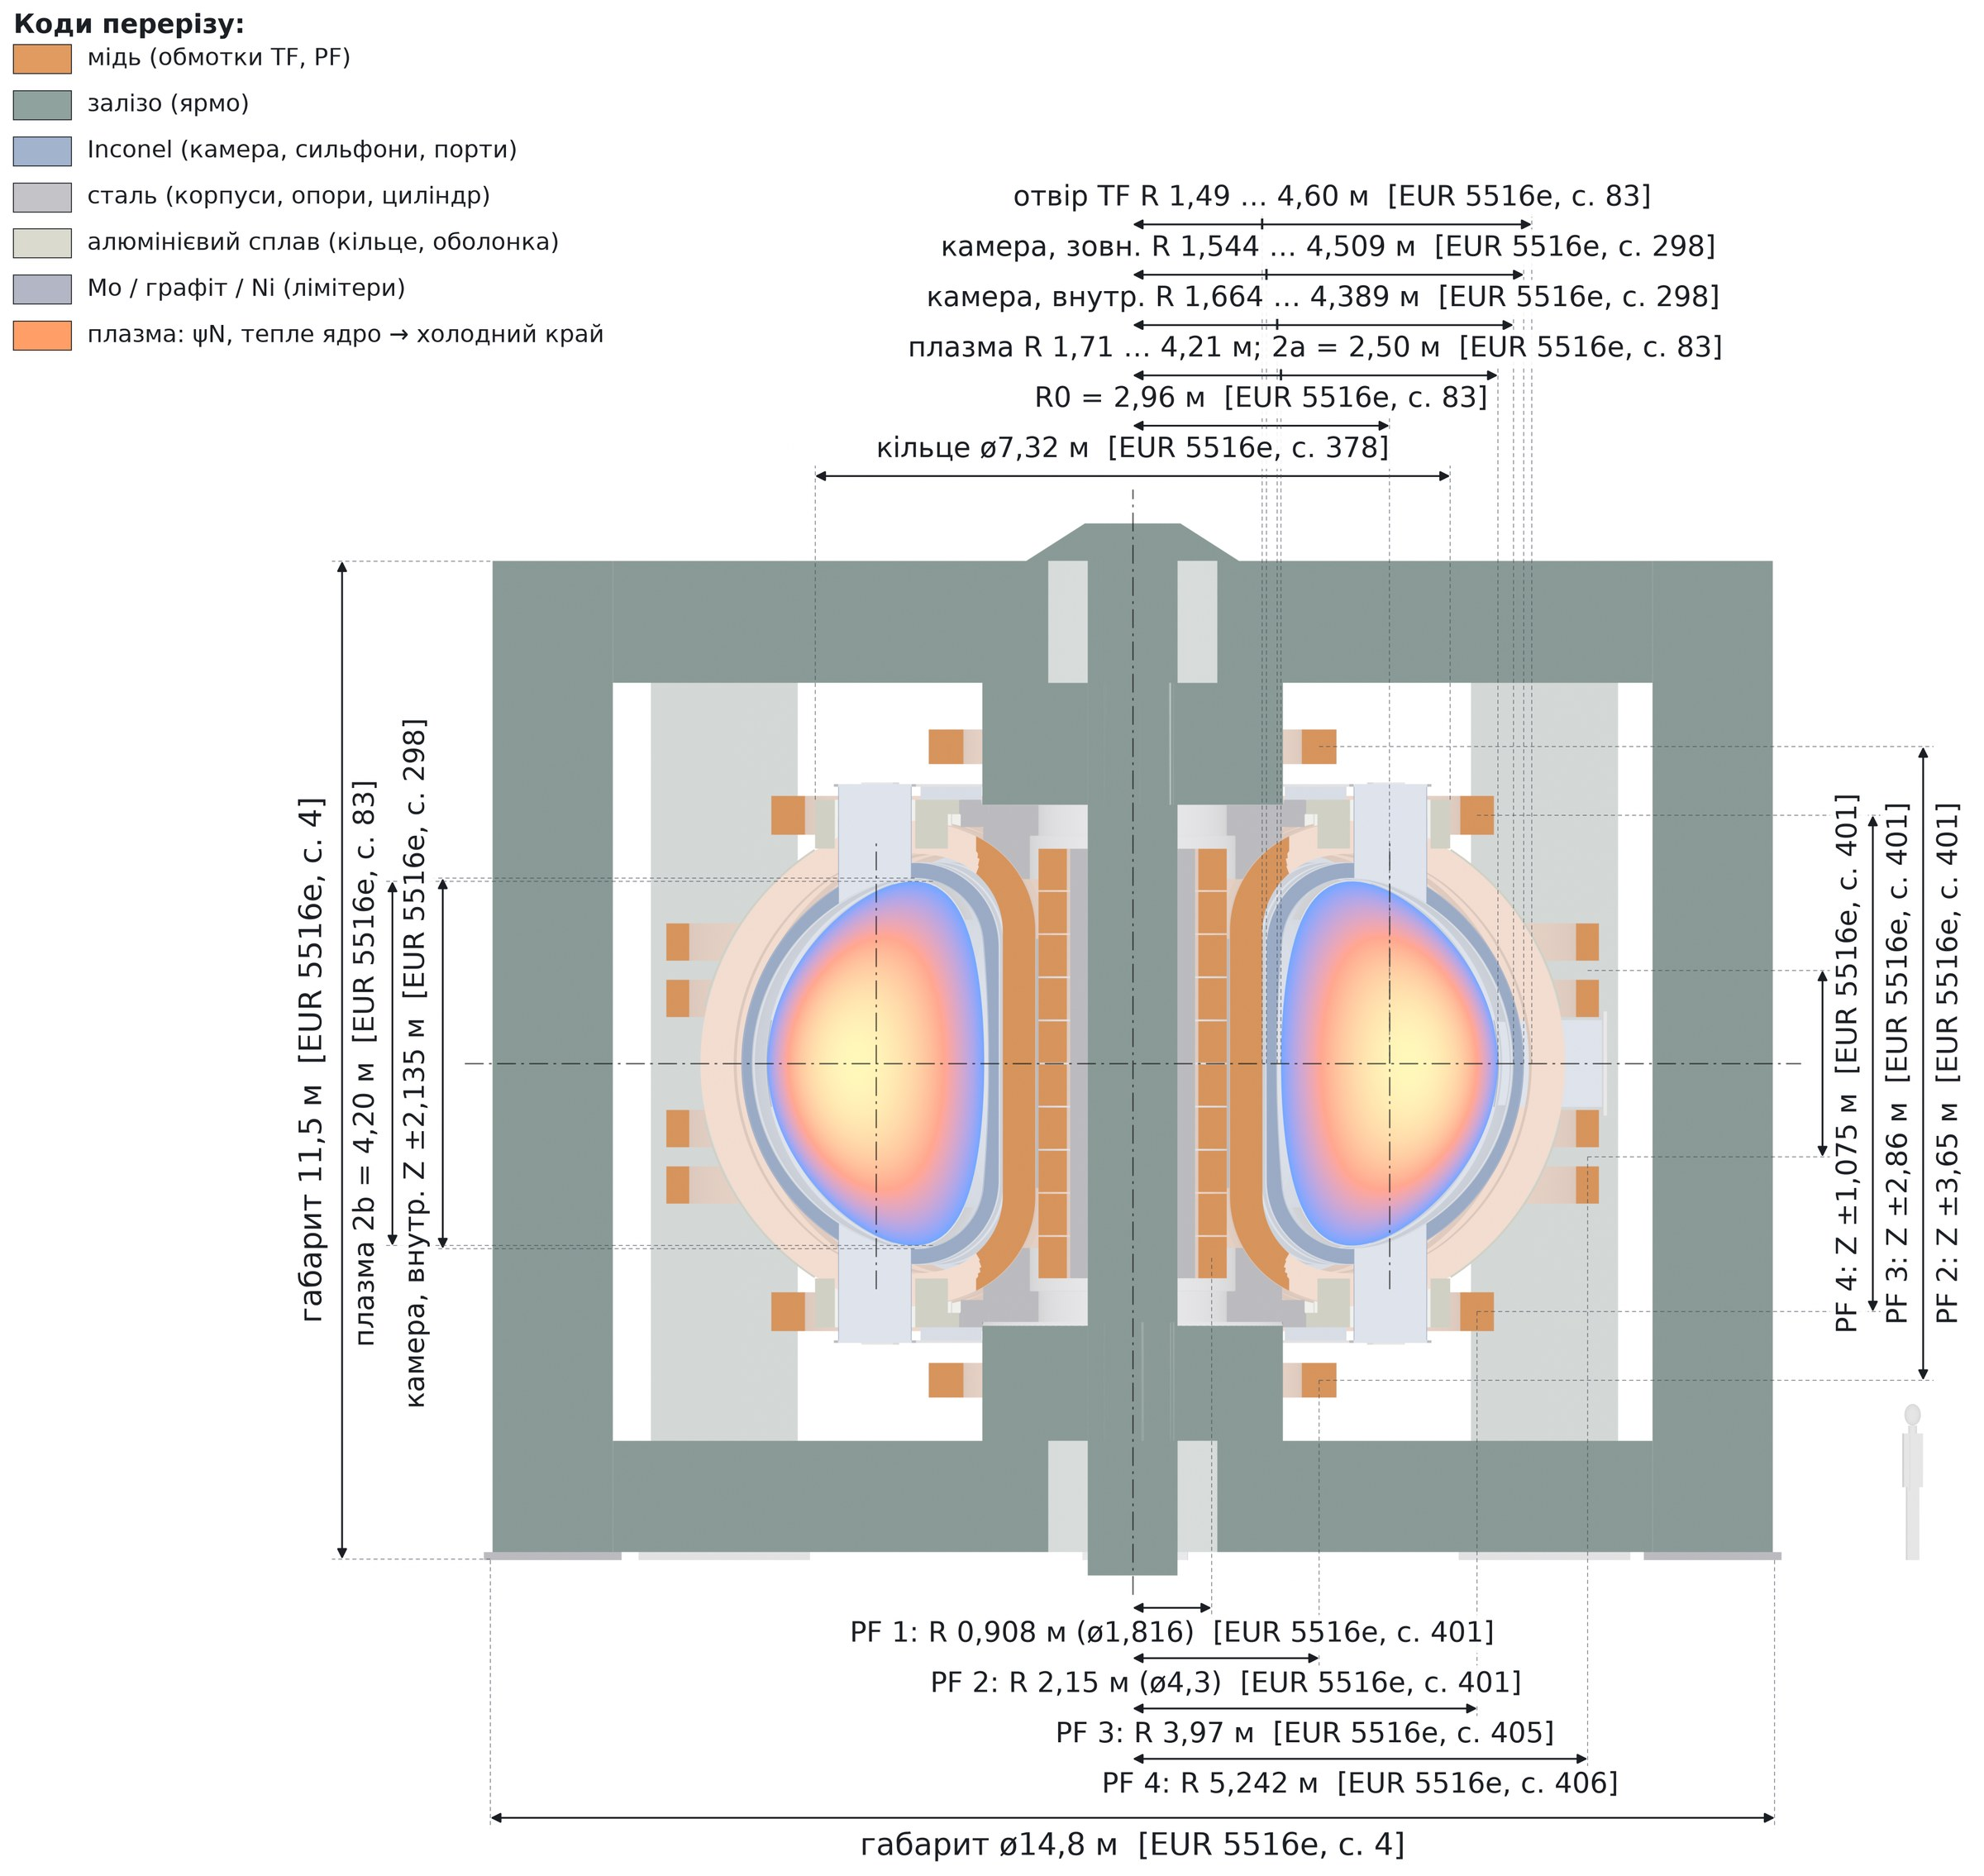
\includegraphics[width=0.88\textwidth]{jet_section.jpg}
  \caption{Вертикальний переріз JET 1975 через плече ярма. Показано розміри з посиланнями на сторінки джерела; кольори кодують матеріали. Від осі назовні: центральна колона ярма, стек PF-1, внутрішня нога TF, камера, плазма ($\psiN$), зовнішня нога TF, PF-2--4, вертикальні плечі. Власна 3D-реконструкція~\cite{ProjJET}; побудовано за даними~\cite[с.~4, 83, 298, 378, 401, 405--406]{JET1975}.}
  \label{fig:04j-section}
\end{figure}

\paragraph{Плазма і перша стінка.} Межа плазми лежить на $R=1{,}71\ldots\SI{4,21}{м}$. Від внутрішньої стінки жорсткого сектора її відділяють \SI{5}{см}, від зовнішньої --- \SI{16}{см}~\cite[с.~83]{JET1975}. Плазма має торкатися не стінки, а лімітерів. У проєкті 1975~р. їх два види. Основні --- три кільцеві «рейки» з окремих пластин уздовж тора; пластини охолоджує потік газу, і їхнє положення можна підправляти ззовні, не відкриваючи камеру~\cite[с.~301]{JET1975}. Зовнішню рейку складали 16 молібденових пластин $100\times60\times\SI{1}{см}$, разом близько тонни Mo~\cite[с.~314]{JET1975}. Допоміжні --- полоїдальні екрани біля кожного сильфона на $R=1{,}70$ і \SI{4,33}{м}: тонкостінні сильфони найвразливіші, зокрема до утікачів~\cite[с.~83, 301]{JET1975}. Уже в проєкті матеріал лімітера вважали «експериментальним параметром», і важкий метал могли замінити на легкий~\cite[с.~301, 315]{JET1975}. У 1983~р. так і сталося (п.~\ref{sec:04j-1983}).

\paragraph{Вакуумна камера.} Форму камери диктує магніт: до котушок TF лишено лише зазори на монтаж, теплоізоляцію і рух стінок під час прогріву й навантаження. Конструкція цілком металева й зварна, як того вимагає надвисокий вакуум~\cite[с.~295]{JET1975}. Стінка --- «коробка» з двох обшивок інконелю: 20~мм на прямій внутрішній ділянці, 12~мм далі по периметру; разом з проміжком це \SI{12}{см} на екваторі й до \SI{18}{см} угорі~\cite[с.~298, 310]{JET1975}. По тору чергуються два типи елементів. Жорсткі клиноподібні сектори (їх 32, по одному на котушку TF) несуть усі сили й мають отвори портів. Між ними стоять сильфонні вставки: пара вкладених один в один сильфонів з листа \SI{1,7}{мм}, проміжок між якими має окреме відкачування на випадок течі внутрішнього сильфона~\cite[с.~295, 306]{JET1975}. Одиниця збирання --- октант із чотирьох секторів і чотирьох сильфонів; шов між октантами проходить посередині крайнього сектора, тому пошкоджений октант можна вирізати й замінити дистанційно цілим модулем~\cite[с.~297, 299]{JET1975}. Маса камери \SI{68}{т}, об'єм $\approx\SI{190}{м^3}$. Площа внутрішньої поверхні --- $\approx\SI{220}{м^2}$ для гладкого тора, $\approx450$ з гофрами сильфонів і $\approx\SI{780}{м^2}$ з екранами й портами~\cite[с.~310]{JET1975}. Цільовий базовий тиск --- $2\cdot10^{-10}$~Торр ($\approx\SI{2,7e-8}{Па}$)~\cite[с.~315]{JET1975}.

\emph{Навіщо сильфони? Тороїдальний опір.} Камера --- замкнений провідний виток навколо того самого осердя трансформатора, що й плазма. Тому напруга обходу $\Vloop$ (розд.~\ref{ch:trap}) наводить у ній паралельний струм $I_{\mathrm v}=\Vloop/\Rv$. Цей струм марно витрачає вольт-секунди, спотворює полоїдальне поле біля плазми і створює сили на камеру. Сильфони мають мале січення й довгий гофрований шлях струму, тож саме вони задають опір камери «довгим шляхом навколо тора». Його свідомо роблять якомога більшим, щоб струм ішов через газ, а не через стінки~\cite[с.~295]{JET1975}, \cite[с.~12]{JETBrochure1982}: $\Rv=\SI{0,52}{мОм}$, індуктивність $\Lv\approx\SI{2,5}{мкГн}$~\cite[с.~304, 310]{JET1975}. Це приблизно вп'ятеро більше за опір водневої плазми з $T_e=\SI{5}{еВ}$, яка заповнює всю камеру~\cite[с.~304]{JET1975}. Отже, на пробої струм іде переважно в плазму. Стала часу $\Lv/\Rv\approx\SI{4,8}{мс}$ задає, як швидко камера «перехоплює» струм під час раптового зриву; для найгіршого випадку проєкт приймав, що в камеру переходить увесь $\Ip$~\cite[с.~304]{JET1975}. У полоїдальному напрямку всі жорсткі сектори ввімкнено паралельно, тож опір там малий (\SI{0,03}{мОм}). Під час наростання $\Btor$ це дає вихрові струми й тиск на стінки сектора~\cite[с.~303--304, 310]{JET1975}.

\begin{outofcorpus}[дві оцінки для камери]
\emph{Без сильфонів.} Уявімо суцільну подвійну обшивку з інконелю ($\rhoe\approx\SI{1,0e-6}{Ом.м}$) із середньою товщиною $2\times\SI{15}{мм}$ на полоїдальному периметрі $\approx\SI{11}{м}$. Для кола довжиною $2\pi R_0$ це дає $\mathcal{R}\approx\rhoe\,2\pi R_0/(0{,}33~\text{м}^2)\approx\SI{0,06}{мОм}$, тобто вдев'ятеро менше, ніж з сильфонами. \emph{Плазма на пробої.} Спітцерівський опір $\eta\approx5{,}2\cdot10^{-5}\lnL/T_e^{3/2}$~Ом$\cdot$м ($T_e$ в еВ) при $T_e=\SI{5}{еВ}$, $\lnL\approx10$ і перерізі камери $\approx\SI{9}{м^2}$ дає $\approx\SI{0,1}{мОм}$. Відношення $\approx5$ збігається з наведеним у проєкті.
\end{outofcorpus}

\emph{Прогрів.} Щоб досягти надвисокого вакууму, камеру прогрівають до \SI{500}{\degreeCelsius} гарячим інертним газом, який проганяють через простір між обшивками. Ззовні камеру вкрито теплоізоляцією товщиною \SI{2,5}{см}~\cite[с.~299, 310, 320]{JET1975}. Теплове розширення становить $\approx\SI{30}{мм}$~\cite[с.~312]{JET1975}, і всі зазори до котушок розраховано з цим запасом (перевірте це в задачі~2).

\paragraph{Котушки TF.} Магніт утворюють 32 D-подібні мідні котушки з водяним охолодженням. Кожна котушка складається з двох «млинців» по 12 витків~\cite[с.~323--324]{JET1975}; габарит $5{,}68\times\SI{3,86}{м}$, маса \SI{12}{т}~\cite[с.~327]{JET1975}, увесь магніт важить $\approx\SI{400}{т}$~\cite[с.~323]{JET1975}. Внутрішні ноги мають клиноподібний переріз і змикаються навколо центрального стека PF. Тому мідь усередині має лише 70\,\% перерізу зовнішньої частини (2700 проти \SI{3900}{мм^2} на виток)~\cite[с.~324, 327]{JET1975}. Струм \SI{53,4}{кА} на виток ($\ITF=\SI{41}{МА}$) дає $\Bzero=\SI{2,77}{Тл}$ на $R=\SI{2,96}{м}$. Розширений режим --- \SI{66,4}{кА} (\SI{51}{МА}, \SI{3,45}{Тл}). Запасена енергія становить 0,94 і \SI{1,45}{ГДж}, повна індуктивність \SI{0,66}{Гн}~\cite[с.~328]{JET1975}. Кожну котушку тягне до осі доцентрова сила $1216$~тс ($\approx\SI{11,9}{МН}$), а в розширеному режимі --- $1880$~тс. Цю силу сприймає клиноподібний «носик» внутрішньої ноги, що впирається в сусідні котушки та центральну опору~\cite[с.~335, 339]{JET1975}.

\paragraph{Механічна структура.} Власне поле TF навантажує котушку лише в її площині. Інша справа --- полоїдальне поле: воно перетинає котушку, і сила $I_1\,\dd\vect{l}\times\Bvec_{\mathrm p}$ напрямлена вже по $\tor$. Оскільки $\BR$ вище й нижче екватора має різні знаки, ця сила тягне верхню й нижню половини котушки в протилежні боки по $\tor$, а від усіх 32 котушок складається крутний момент навколо вертикальної осі~\cite[с.~359]{JET1975}. Його сприймають тонка оболонка з клинових блоків між котушками, верхнє й нижнє кільця ($\varnothing\,\SI{7,32}{м}$, висота \SI{0,9}{м}, по 8 секторів) і внутрішній циліндр з 8 секторів нержавіючої сталі завтовшки в середньому \SI{4}{см}~\cite[с.~364, 374--378]{JET1975}. У збудованій машині оболонку й кільця відлито з немагнітного аустенітного високоміцного чавуну (з кулястим графітом), а внутрішній циліндр зроблено зі сталі 304 з 32 пазами під ноги котушок. Структура важить $\approx\SI{470}{т}$ і розрахована на момент \num{20000}~тс$\cdot$м ($\approx\SI{2e8}{Н.м}$) при закручуванні оболонки не більш ніж на \SI{4}{мм}~\cite[с.~16--17]{JETBrochure1982}.

\paragraph{Котушки PF.} Полоїдальну систему поставлено \emph{ззовні} котушок TF. Так дві системи не зачеплені топологічно, і будь-яку з них можна розібрати, не чіпаючи іншої~\cite[с.~72]{JET1975}. 16 мідних котушок чотирьох типів (табл.~\ref{tab:04j-pf}) утворюють первинну обмотку трансформатора (PF-1) і котушки рівноваги та форми (PF-2--4)~\cite[с.~385, 399]{JET1975}. Для швидких процесів обмотки діють як паралельні контури: різкий зсув плазми змінює їхнє потокозчеплення, і наведені струми (правило Ленца) тягнуть її назад, як суцільна мідна оболонка~\cite[с.~385]{JET1975} (розд.~\ref{ch:stability}).

\begin{table}[!tb]\centering\small\setlength{\tabcolsep}{5pt}
\caption{Котушки PF JET у проєкті 1975~р.~\cite[с.~401]{JET1975}}\label{tab:04j-pf}
\begin{tabular}{@{}lcccc@{}}
\toprule
 & PF-1 (внутр.) & PF-2 (внутр.) & PF-3 (зовн.) & PF-4 (зовн.) \\
\midrule
Кількість & 10 & 2 & 2 & 2 \\
Середній діаметр, м & 1,816 & 4,3 & 7,94 & 10,486 \\
Відстань від екватора $\pm Z$, м & --- (стек) & 3,65 & 2,86 & 1,075 \\
Витків (послідовно) на котушку & 63 & 48 & 120 & 96 \\
Макс.\ струм у провіднику, кА & 34 & 34 & 11,8 & 13 \\
Маса міді на котушку, т & 5,7 & 10 & 20,2 & 35,9 \\
\bottomrule
\end{tabular}
\end{table}

\paragraph{Залізне осердя трансформатора.} Струм у плазмі наводиться трансформатором: $\Vloop=-\dd\Phi/\dd t$, де $\Phi$ --- потік, зчеплений з плазмовим витком. Ярмо --- це 8 вертикальних плечей, 8 верхніх і 8 нижніх радіальних плечей, два центральні блоки й центральна колона, разом 27 основних деталей і \SI{2263}{т}~\cite[с.~415]{JET1975}. Навіщо залізо, якщо центральна колона все одно насичується? Зовнішній контур з ненасиченого заліза ($B<\SI{1,9}{Тл}$) дає потоку короткий шлях повернення. Через це машині потрібно лише $\approx2/3$ струму намагнічування і $\approx1/2$ енергії порівняно з еквівалентною машиною без заліза~\cite[с.~399, 411]{JET1975}. Крім того, залізо притримує поле розсіювання навколо машини~\cite[с.~385]{JET1975}. Це важливо для інжекторів: уже $\sim$\SI{1}{мТл} (10~Гс) заважає їхній роботі, а біля зовнішніх плечей очікували $\sim$\SI{20}{мТл}~\cite[с.~419]{JET1975}. Ціна малого $R_0/a$ --- брак місця в центрі: на колону лишається малий переріз, і в базовому режимі залізо там насичене до \SI{6,6}{Тл}~\cite[с.~385, 412]{JET1975}. Другий прийом --- використати петлю намагнічування з обох боків: перед імпульсом осердя заздалегідь намагнічують «від'ємно», і під час наростання струму потік проходить від $-15$ до $+\SI{10}{Вб}$, тобто майже вдвічі більший перепад за тих самих струмів котушок~\cite[с.~411--412]{JET1975}. Перепад \SI{25}{Вб} і дорівнює проєктному запасу \SI{25}{В.с}~\cite[с.~83]{JET1975}.

\paragraph{Порти й доступ.} Кожен октант має великий горизонтальний порт в екваторіальній площині з отвором $0{,}46\times\SI{0,96}{м}$. Через нього пучок нейтралів діаметром до \SI{280}{мм} можна ввести під кутом $45^\circ$ до осі~\cite[с.~301]{JET1975}. Вертикальні наскрізні порти мають розміри $14\times83$ і $7\times\SI{28}{см}$~\cite[с.~77]{JET1975}. На чотирьох із восьми горизонтальних портів стоять насосні блоки~\cite[с.~315]{JET1975}. Концепція нагріву 1975~р. передбачала шість квазітангенціальних інжекторів на один порт~\cite[с.~426]{JET1975} з енергією $\ge\SI{80}{кеВ}$ (H) і нарощуванням потужності до $\sim\SI{25}{МВт}$~\cite[с.~418]{JET1975}. Уся машина має габарит $\varnothing\,14{,}8\times\SI{11,5}{м}$~\cite[с.~4]{JET1975} і масу близько \SI{3000}{т}, яку несуть нижні плечі ярма~\cite[с.~414]{JET1975}.

\begin{figure}[!tb]\centering
  \begin{subfigure}{0.495\textwidth}\centering
    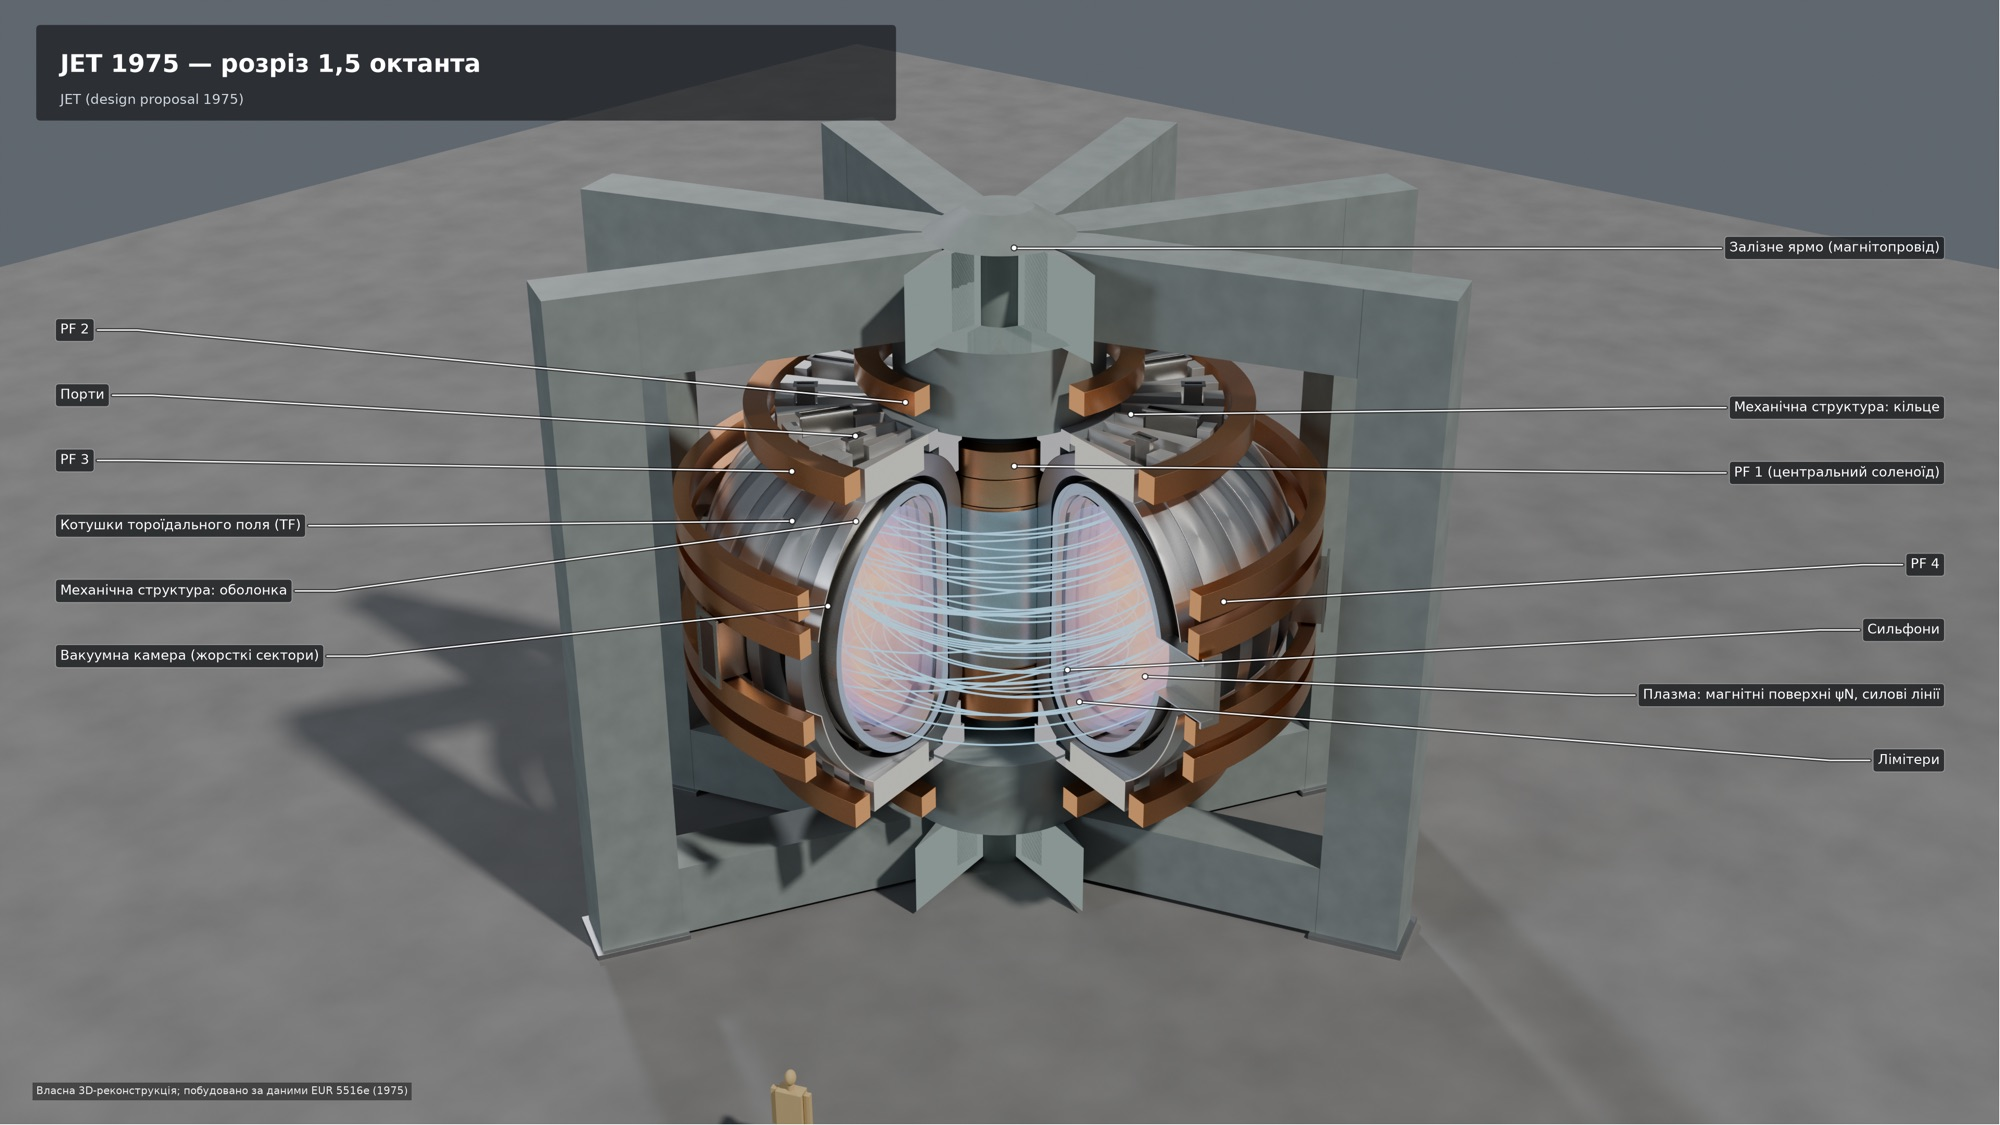
\includegraphics[width=\textwidth,trim=0 40 0 130,clip]{jet_cutaway1975.jpg}\caption{}
  \end{subfigure}\hfill
  \begin{subfigure}{0.495\textwidth}\centering
    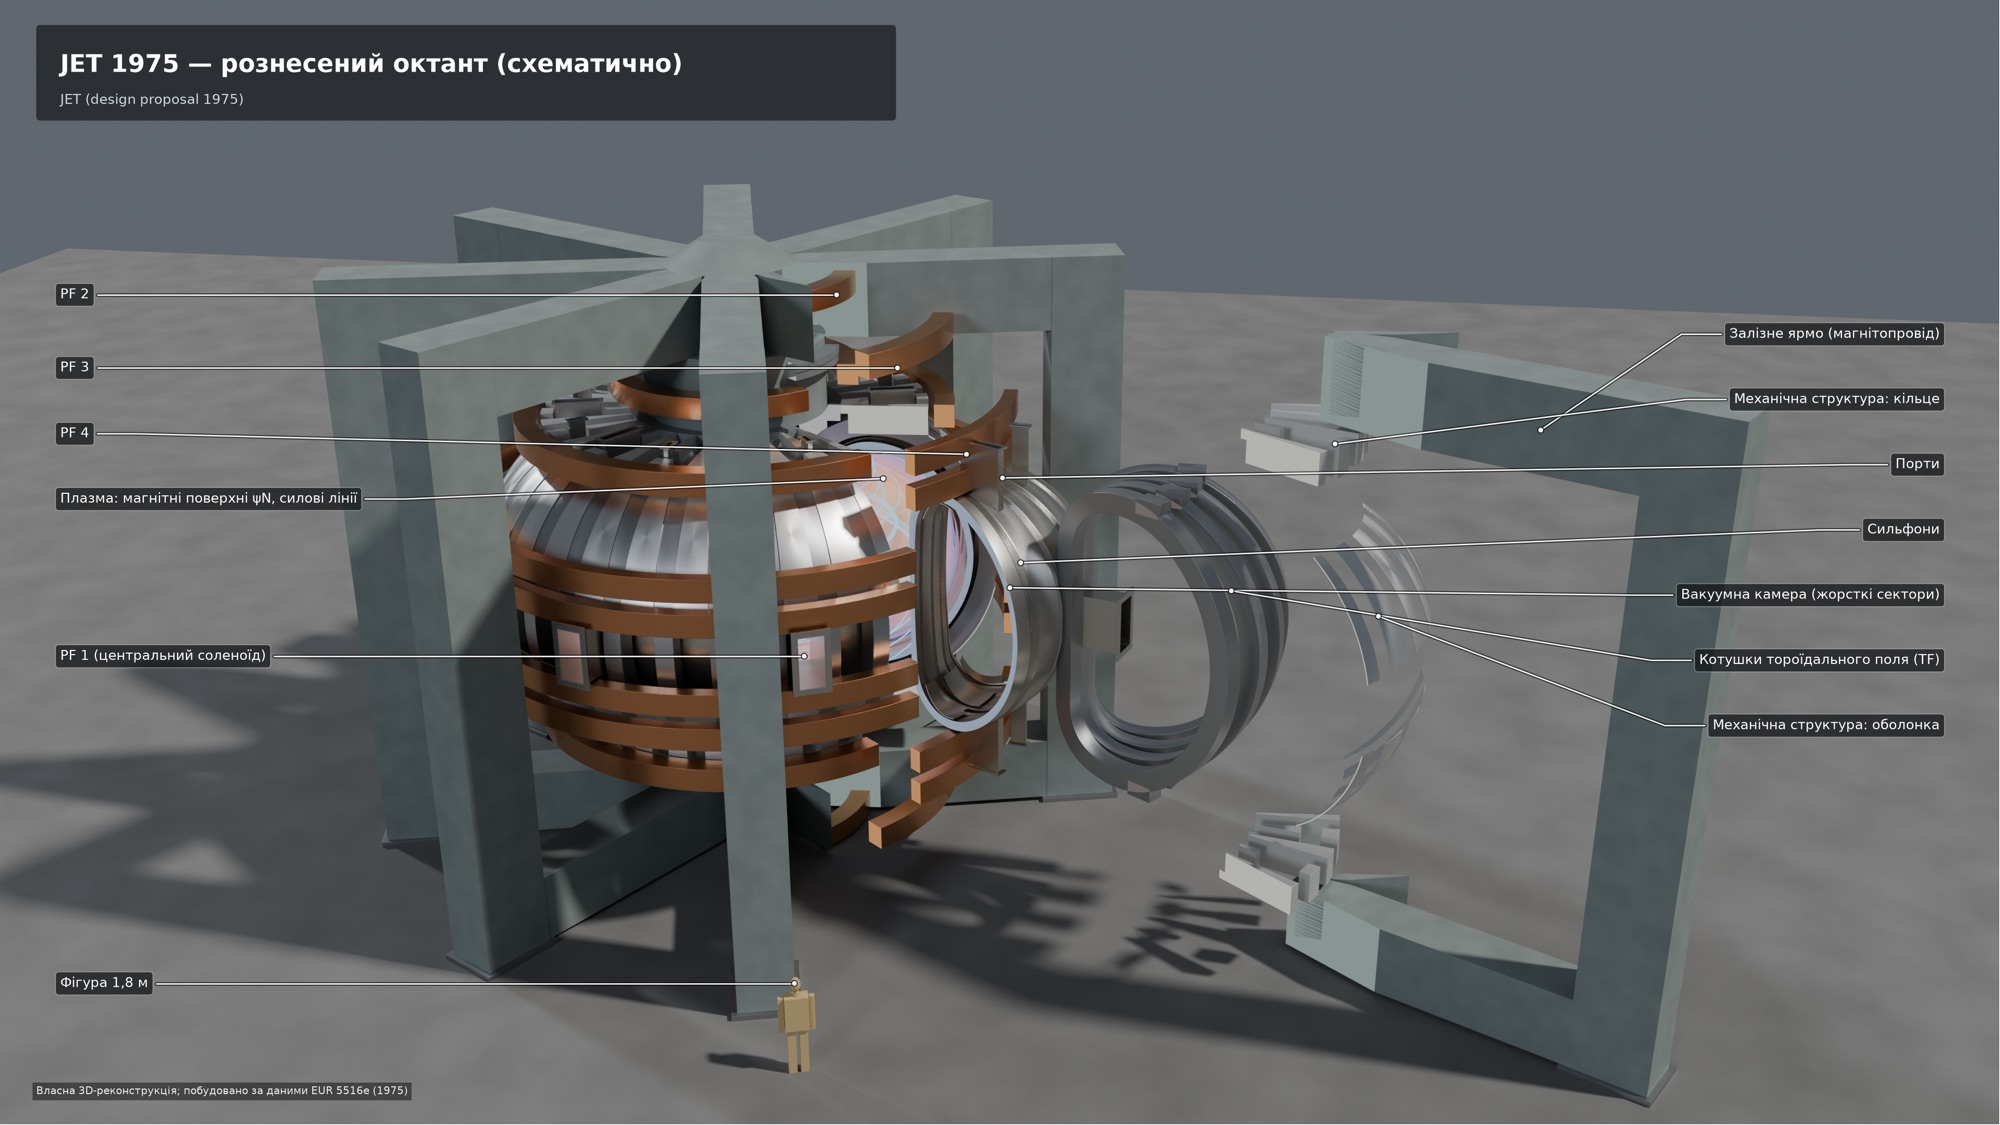
\includegraphics[width=\textwidth,trim=0 40 0 130,clip]{jet_exploded.jpg}\caption{}
  \end{subfigure}
  \caption{JET 1975: (a)~розріз на 1,5 октанта (ярмо, PF-1--4, котушки TF, оболонка, камера із сильфонами, плазма з силовими лініями); (b)~схематично рознесений октант --- одиниця збирання й дистанційної заміни (ярмо, кільце, оболонка, котушки TF і сектор камери зсунуто назовні). Людська фігура --- \SI{1,8}{м}. Власна 3D-реконструкція~\cite{ProjJET}; побудовано за даними~\cite[с.~4, 83, 295--299, 325, 378, 401, 415]{JET1975}.}
  \label{fig:04j-cutaway}
\end{figure}

\section{Гофрування поля 32 котушок}\label{sec:04j-ripple}

Скінченне число котушок робить $|\Bvec|$ періодичним по $\tor$ з періодом $2\pi/32$. Чим це загрожує швидким частинкам, розглянуто в п.~\ref{sec:02-ripple} (розд.~\ref{ch:particles}). Число котушок JET обрано саме з умови однорідності поля~\cite[с.~13]{JETBrochure1982}, а ще на початку проєктування гофрування рахували для кількох розкладок~\cite[с.~329]{JET1975}. \emph{Пастка в означеннях.} Сучасна глибина гофрування --- $\dripple=(B_{\max}-B_{\min})/(B_{\max}+B_{\min})$, де $B_{\max}$ береться в площині котушки, а $B_{\min}$ --- посередині між котушками. Але проєкт JET у підписі до графіка гофрування визначає $\eripple=2(B_{\max}-B_{\min})/(B_{\max}+B_{\min})=2\dripple$~\cite[с.~330]{JET1975}. Отже, проєктне «гофрування 3,6\,\%» на краю плазми~\cite[с.~83]{JET1975} означає $\dripple\approx1{,}8\,\%$.

\begin{projmodel}[гофрування за Біо--Саваром]
Кожну з 32 котушок представлено ниткою вздовж осьової лінії обмотки: оцифрований контур отвору~\cite[с.~325]{JET1975}, зсунутий на половину товщини ноги (\SI{0,186}{м}). Струм --- \SI{41}{МА}. Результат~\cite{ProjJET} (рис.~\ref{fig:04j-ripple}):
\begin{itemize}
\item $\eripple(\SI{4,21}{м})=3{,}67\,\%$ (з $3\times3$ нитками на котушку 3,74\,\%) проти проєктних 3,6\,\%; на осі $\dripple\approx3\cdot10^{-7}$;
\item уздовж 30 точок межі з таблиці проєкту~\cite[с.~332]{JET1975} відношення «наше/джерело» становить у середньому 0,97 (0,90--1,10);
\item незалежна перевірка: $B(R_0)=\SI{2,770}{Тл}$ при \SI{41}{МА} і \SI{3,446}{Тл} при \SI{51}{МА}, як у проєкті (2,77 і 3,45).
\end{itemize}
Головна невизначеність --- сама форма котушки. Радіуси D на кресленні не надруковано, і контур оцифровано з похибкою $\pm10\ldots\SI{20}{мм}$. Біля краю гофрування зростає приблизно в $\ee$ разів на кожні $R/N\approx\SI{0,13}{м}$, тому зсув осьової лінії на $\pm\SI{2}{см}$ змінює $\eripple(\SI{4,21}{м})$ до 4,18 і 3,22\,\% ($+14/-12\,\%$). При $R<\SI{4,1}{м}$ наші значення на 20--35\,\% нижчі за оцифровану криву джерела. Але там $\eripple<2\,\%$, і сама товщина лінії на рисунку ($\pm0{,}1\,\%$) порівнянна з різницею.
\end{projmodel}

\begin{figure}[!tb]\centering
  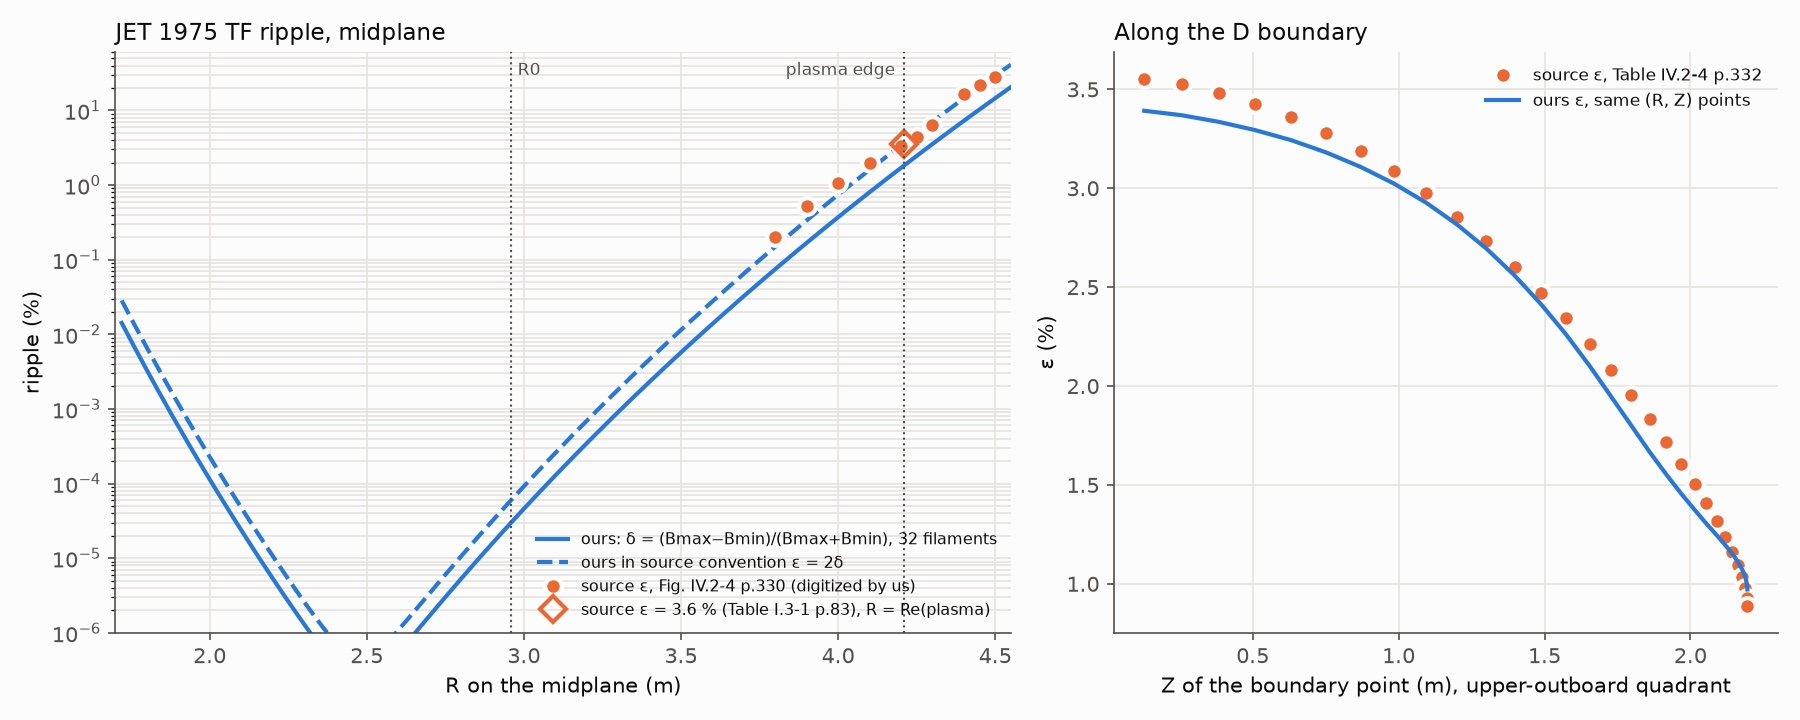
\includegraphics[width=\textwidth]{jet_ripple.jpg}
  \caption{Гофрування TF-поля JET 1975. Ліворуч --- на екваторі, логарифмічна шкала: наше $\dripple$ (суцільна), наше $\eripple=2\dripple$ (штрихова), точки --- значення, оцифровані нами з графіка гофрування~\cite[с.~330]{JET1975}, ромб --- 3,6\,\% на $R=\SI{4,21}{м}$~\cite[с.~83]{JET1975}. Праворуч --- $\eripple$ уздовж верхньої зовнішньої чверті межі: точки з таблиці~\cite[с.~332]{JET1975}, лінія --- наш розрахунок у тих самих точках. Власний розрахунок~\cite{ProjJET}.}
  \label{fig:04j-ripple}
\end{figure}

Чому гофрування так круто зростає назовні? Грубо кажучи, поле окремих ниток котушок, розташованих з кроком $2\pi R/N$ по колу радіуса $R_2$, спадає всередину як $(R/R_2)^N$, а від внутрішніх ніг на $R_1$ --- як $(R_1/R)^N$ (стандартна оцінка, поза корпусом). Для $N=32$, $R_1=\SI{1,30}{м}$, $R_2=\SI{4,79}{м}$ це дає $\dripple(\SI{4,21}{м})\approx(4{,}21/4{,}79)^{32}\approx1{,}6\,\%$ проти 1,83\,\% за Біо--Саваром. Для порівняння, у моделі ITER з розд.~\ref{ch:particles} на межі плазми $\dripple=4{,}5\cdot10^{-3}$. Плазма JET заповнює отвір майже до зовнішньої ноги, і за це доводиться платити гофруванням.

\section{Рівновага плазми в геометрії JET}\label{sec:04j-eq}

Щоб показати в реконструкції магнітні поверхні й силові лінії, потрібна рівновага в межах проєктної D-межі (розд.~\ref{ch:equilibrium}). Ми взяли найпростішу точну: розв'язок Соловйова.

\begin{outofcorpus}[рівновага Соловйова у формі Cerfon--Freidberg]
Якщо $\mu_0p'(\psi)$ і $FF'(\psi)$ сталі, рівняння $\GSop\psi=-\mu_0R^2p'-FF'$ стає лінійним. У змінних $x=R/R_0$, $y=Z/R_0$, $\psi=\psi_0u$ його розв'язок --- частинний поліном плюс сума семи однорідних розв'язків, парних по $y$. Сім коефіцієнтів визначають так, щоб межа $u=0$ проходила через три точки D-контуру (зовнішній і внутрішній екватор, верх) з правильними нахилом і кривинами~\cite{Cerfon2010}. Густина струму $\Jtor=(C_1R+C_2/R)/\mu_0$ від $\psi$ не залежить, тобто профіль \emph{плаский}.
\end{outofcorpus}

Межу задано у формі Міллера з $R_0$, $a$, $b$ проєкту та трикутністю $\delta=0{,}348$, підігнаною до форми межі з таблиці гофрування~\cite[с.~332]{JET1975}. Така плазма лежить у камері з зазорами 18 і \SI{5}{см}~\cite{ProjJET}. Сама таблиця суперечлива: її верхня точка ($Z=\SI{2,195}{м}$) на \SI{9,5}{см} вища за $b$ і виходить за стінку. Залишаються два вільні параметри. Поділ струму між $p'$ і $FF'$ вибрано так, щоб $\betap=0{,}9$, як у виносках проєкту, а масштаб $\psi$ --- так, щоб $\Ip=\SI{3,8}{МА}$~\cite[с.~83]{JET1975}. Результати --- у табл.~\ref{tab:04j-eq}.

\begin{table}[!tb]\centering\small
\caption{Рівновага Соловйова в межі JET 1975 (наш розрахунок~\cite{ProjJET}) і проєктні значення~\cite[с.~83]{JET1975}}\label{tab:04j-eq}
\begin{tabular}{@{}lll@{\hspace{2em}}lll@{}}
\toprule
Величина & Модель & Проєкт & Величина & Модель & Проєкт\\
\midrule
$\Ip$, МА & 3,80 & 3,8 & $\qnf$ & 5,51 & --- \\
$\Bzero$, Тл (вакуум) & 2,770 & 2,77 & $q(a)$ & 5,81 & 6 \\
$\betap$ & 0,90 & 0,9 & $q_0$ & 2,80 & $\approx1$ \\
$\betat$, \% & 2,32 & --- & $\li$ (3) / (1) & 0,425 / 0,498 & --- \\
$\Delta_{\mathrm S}$, м & 0,223 & --- & нев'язка межі, мм & 0,08 & --- \\
\bottomrule
\end{tabular}
\end{table}

Формула~\eqref{eq:04j-qD} дає $q(a)=5{,}99$, модель --- 5,81, тобто на 3\,\% менше. Автори проєкту самі зазначали, що навіть малі зміни форми перерізу змінюють $k$ і $q$ до 30\,\%~\cite[с.~83]{JET1975}. Зсув Шафранова можна порівняти з оцінкою з розд.~\ref{ch:equilibrium}: $(a^2/2R_0)(\betap+\li/2)\approx\SI{0,29}{м}$ для круглої плазми з великим аспектним відношенням. Витягнутість його зменшує, і модель дає \SI{0,223}{м}. \emph{Чесне обмеження.} Струм Соловйова плаский, тому $q_0=2{,}80$ і $q(a)/q_0=2{,}1$, а проєкт розраховував на пікований струм з $q(a)/q(0)=5{,}3\ldots6$, тобто $q_0\approx1$~\cite[с.~71, 83]{JET1975}. Тому поверхонь $q=1$, $3/2$ і $2$ у нашій плазмі \emph{немає}, і острів 2/1 тут нерезонансний. Модель придатна для топології (вкладені поверхні, раціональні лінії $q=3,\,7/2,\,4,\,5$ замикаються з точністю $<\SI{0,5}{мм}$), але не для МГД-стійкості. Для реалістичного $q$-профілю потрібен чисельний розв'язувач з $p'(\psi)$ і $FF'(\psi)$, що спадають до межі.

\section{Проєкт 1975 і машина 1983}\label{sec:04j-1983}

Між проєктом і першою плазмою минуло вісім років. Основні параметри плазми й магніту TF не змінилися: $a$, $b$, $R_0$, 32 котушки по 24 витки, \SI{12}{т} кожна, разом \SI{384}{т}~\cite[с.~13]{JETJU1983}, \cite[с.~6, 13]{JETBrochure1982}. Змінилося майже все довкола плазми (табл.~\ref{tab:04j-1983}, рис.~\ref{fig:04j-1983}).

\begin{table}[!tb]\centering\footnotesize\setlength{\tabcolsep}{4pt}\renewcommand{\arraystretch}{1.05}
\caption{Проєкт 1975~р. і машина 1983~р. (сторінки PDF)}\label{tab:04j-1983}
\begin{tabularx}{\textwidth}{@{}l>{\raggedright\arraybackslash}X>{\raggedright\arraybackslash}X@{}}
\toprule
Вузол & 1975~\cite{JET1975} & 1983~\cite{JETJU1983} та ін. \\
\midrule
Октант камери & 4 жорсткі сектори + 4 сильфони; разом 32 сектори (с.~295, 297) & 5 жорстких секторів трьох типів + 4 сильфони; разом 40 (с.~24); так само~\cite[с.~12]{JETBrochure1982} і вже в 1979~р.~\cite[с.~36]{JETJU1979} \\
Сильфони & лист 1,7~мм (с.~306) & лист 2~мм, гофри 120~мм (с.~24) \\
Маса / опір камери & 68~т; 0,52~мОм (с.~310) & 108~т (с.~13); 0,6~мОм (с.~24); кільця жорсткості на $Z=\pm\SI{1}{м}$ (с.~24) \\
Лімітери & 3 рейкові, 16 пластин Mo по $100\times60$~см (с.~301, 314) & 12 модулів по 0,32~м$^2$ на зовнішньому екваторі: 4 графітові + 8 з Ni-плакуванням на CuCr (с.~24); липень--листопад 1983~р. працювали лише 4 графітові (с.~39) \\
PF-1 & 10 котушок (с.~401) & 8 котушок, 40~кА; усього PF 14~\cite[с.~15]{JETBrochure1982} \\
Залізо & 2263~т (розширений варіант 2567~т) (с.~415) & 2800~т (с.~13) \\
Оболонка й кільця & зовнішня частина кільця --- литий легкий сплав (с.~376) & аустенітний високоміцний чавун, $\approx470$~т~\cite[с.~17]{JETBrochure1982} \\
Порти, нагрів & 4 насосні порти з 8 (с.~315); концепція NBI 6~інжекторів на порт (с.~426) & насосні камери на октантах 1 і 5, адаптери NBI на 4 і 8 (с.~24--25); поворотні клапани --- січень 1984~р., перший бокс NBI --- вересень 1984~р. (с.~40); у 1983~р. додаткового нагріву немає \\
Прогрів & до 500\,°C (с.~299) & проєктно 500\,°C; октанти відпалено при 520\,°C (с.~24); у кампаніях 1983~р. --- 270\,°C (с.~13), 300\,°C стінки і 200\,°C порти (с.~39) \\
\bottomrule
\end{tabularx}
\end{table}

\begin{figure}[!tb]\centering
  \begin{subfigure}{0.495\textwidth}\centering
    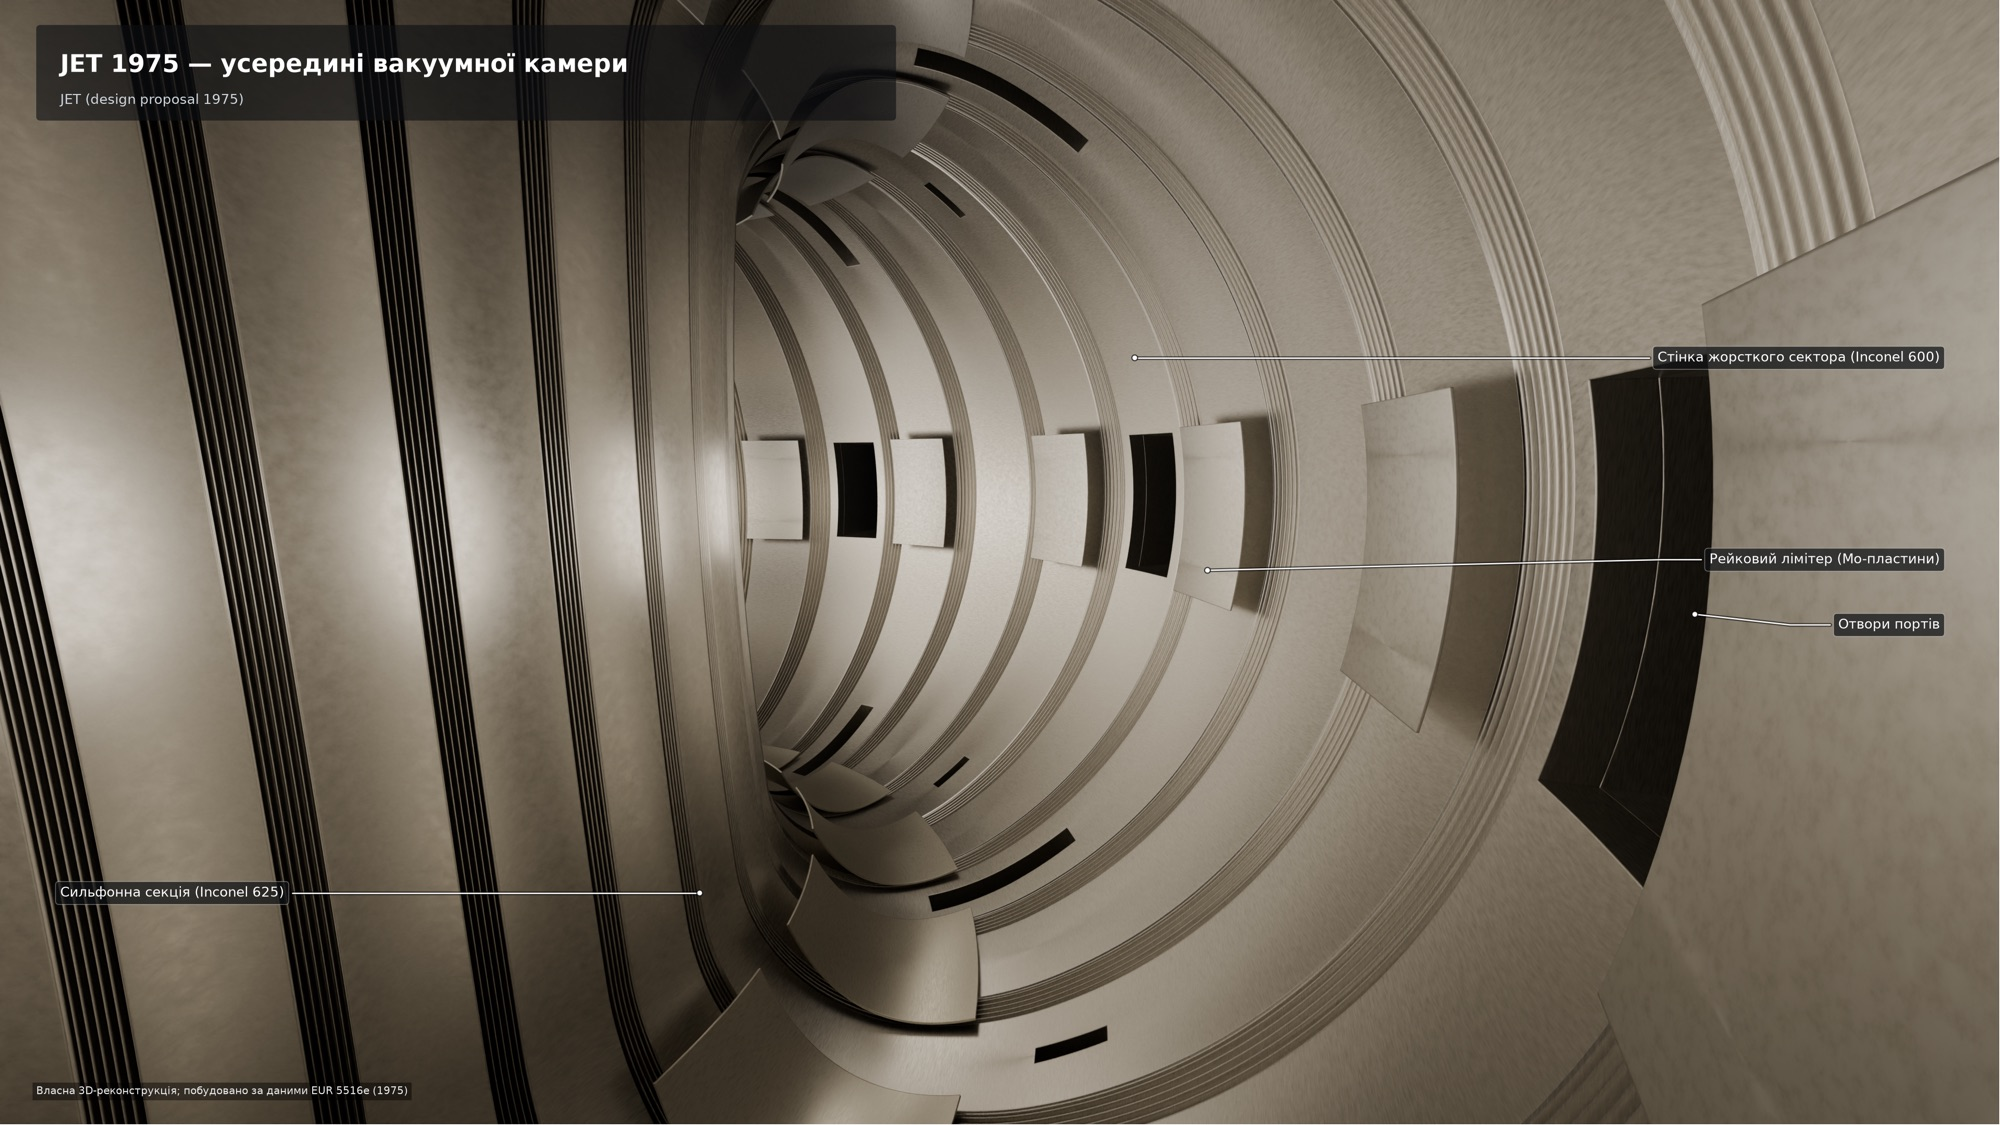
\includegraphics[width=\textwidth,trim=0 40 0 130,clip]{jet_invessel.jpg}\caption{}
  \end{subfigure}\hfill
  \begin{subfigure}{0.495\textwidth}\centering
    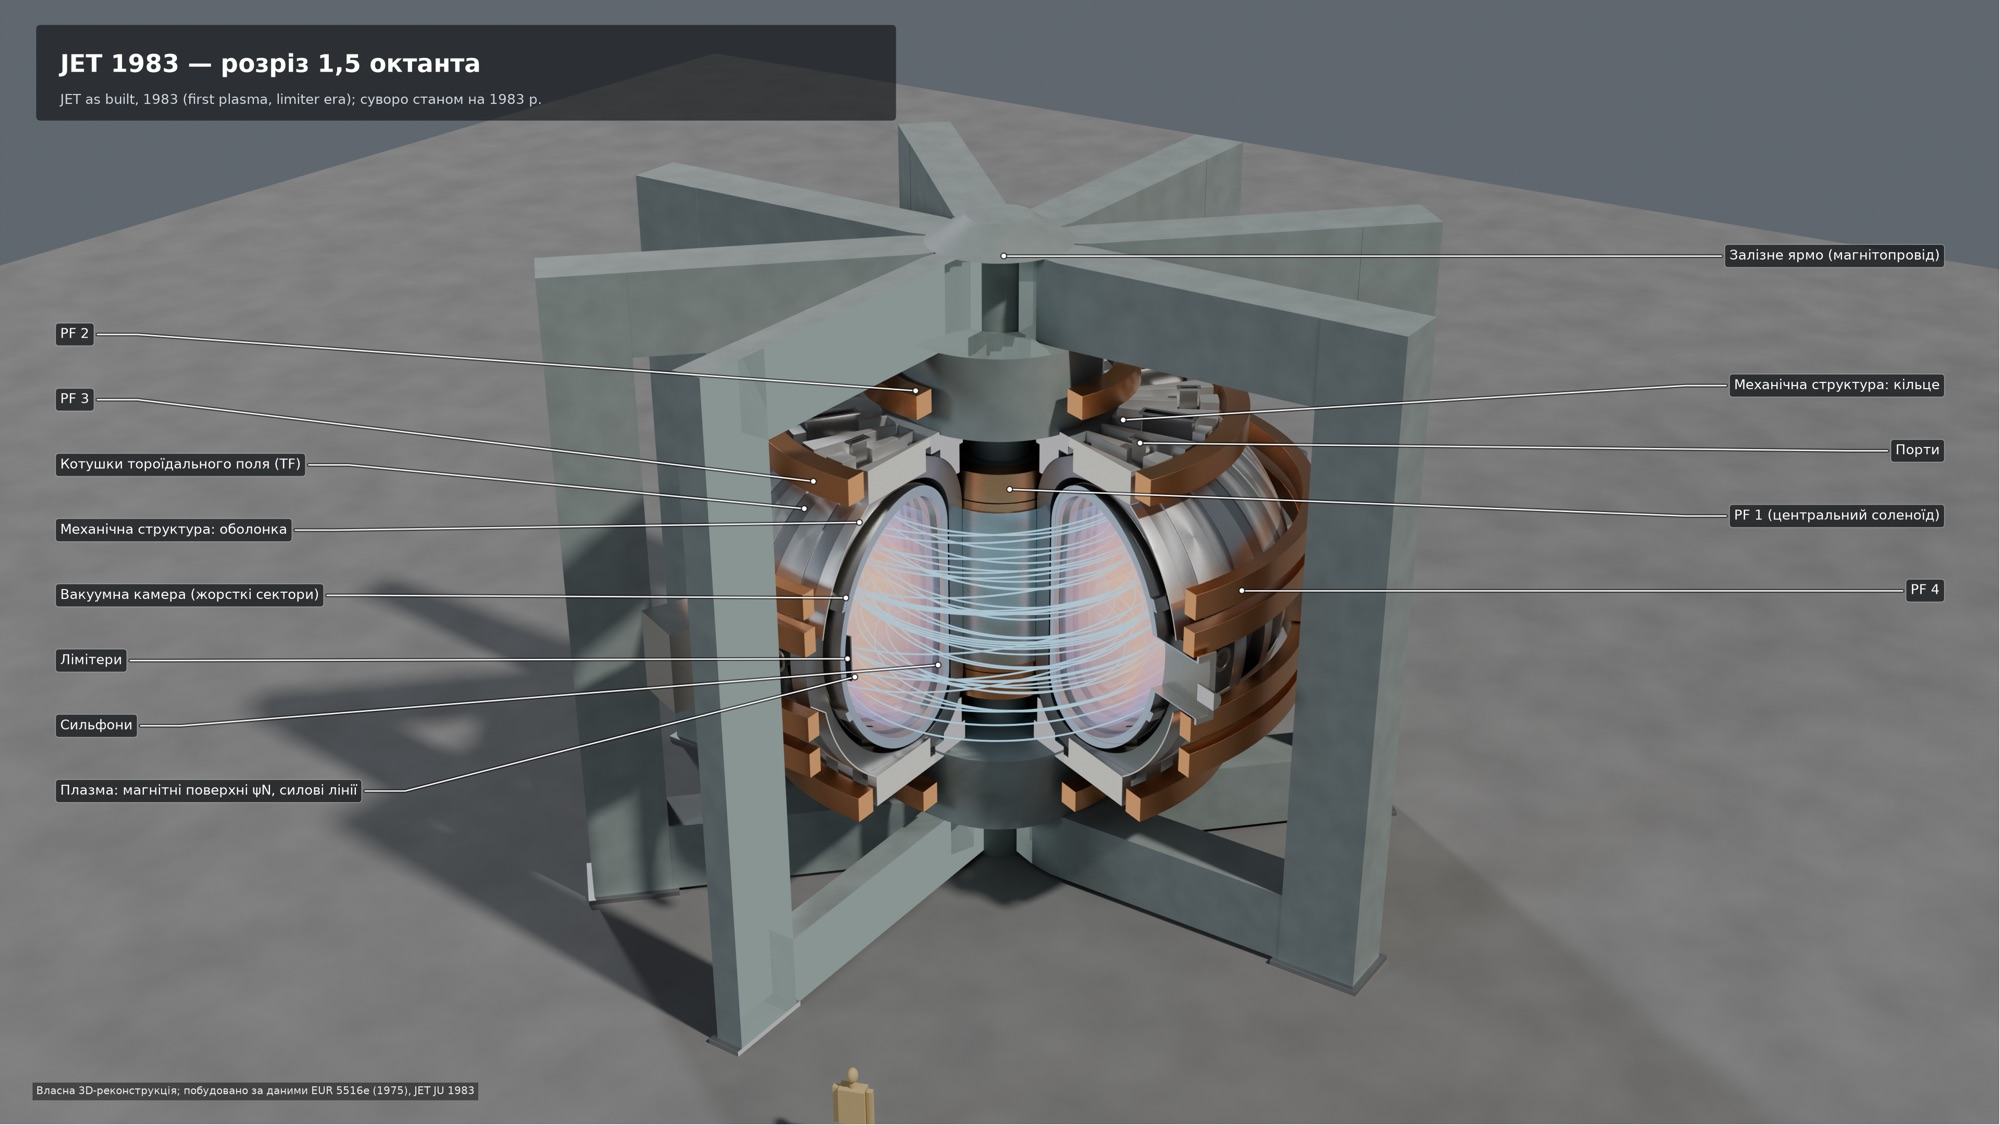
\includegraphics[width=\textwidth,trim=0 40 0 130,clip]{jet_cutaway1983.jpg}\caption{}
  \end{subfigure}
  \caption{(a)~Усередині камери JET 1975: стінки жорстких секторів (Inconel~600), гофровані сильфонні секції (Inconel~625), пластини зовнішнього рейкового Mo-лімітера, отвори портів. (b)~JET 1983 у тому самому ракурсі, що й рис.~\ref{fig:04j-cutaway}a: 40 жорстких частин камери, кільця жорсткості, дискретні модулі лімітера на зовнішньому екваторі, 8 котушок PF-1. Власна 3D-реконструкція~\cite{ProjJET}; побудовано за даними~\cite[с.~295--314]{JET1975} і~\cite[с.~13, 24--25, 39--40]{JETJU1983}.}
  \label{fig:04j-1983}
\end{figure}

Два пояснення до таблиці. \emph{40 жорстких частин при 32-кратній симетрії.} Уже в 1975~р. октанти зварювали посередині крайніх секторів, тож октант був послідовністю $\tfrac12+3+\tfrac12$ сектори~\cite[с.~299]{JET1975}. У 1983~р. ці половинки стали окремими деталями. Так ми тлумачимо «п'ять жорстких секторів» у~\cite[с.~24]{JETJU1983}; це тлумачення зберігає відповідність 32 котушкам TF. \emph{Графіт замість металу.} Проєкт лишав матеріал лімітера відкритим, і в машину поставили і графітові, і нікелеві модулі. Перші розряди 1983~р. були забруднені C і O; після підвищення температури прогріву плазма стала гарячішою, але з'явилися Ni і Cr зі стінки~\cite[с.~13]{JETJU1983}. Нікелеві модулі так і не випробували, а на 1984~р. планували пояскові лімітери й вивчали берилій~\cite[с.~39--40]{JETJU1983} (розд.~\ref{ch:wall}).

\paragraph{Суперечності джерел.} Їх варто знати, щоб не «виправляти» одне джерело іншим.
\begin{itemize}
\item \emph{Розміри камери.} «$4{,}3\times\SI{2,7}{м}$»~\cite[с.~23]{JETJU1983} --- внутрішня обшивка жорсткого сектора ($2\times2{,}135$ і $4{,}389-1{,}664$ за кресленням~\cite[с.~298]{JET1975}). «$2{,}5\times\SI{4,2}{м}$»~\cite[с.~12]{JETJU1983} --- це плазма $2a\times2b$. «$2{,}63\times\SI{4,18}{м}$»~\cite[с.~310]{JET1975}, \cite[с.~13]{JETBrochure1982} --- радіуси екранів сильфонів (4,33~м $-$ 1,70~м). Це три різні поверхні, а не три версії камери.
\item \emph{Маси.} Камера: 108~т~\cite[с.~13]{JETJU1983}, 100~т~\cite[с.~6]{JETBrochure1982}. Залізо: 2263 і 2567~т~\cite[с.~415]{JET1975}, 2567~т~\cite[с.~15]{JETJU1979}, 2700~т~\cite[с.~18]{JETBrochure1982}, 2800~т~\cite[с.~13]{JETJU1983}, 2600~т~\cite[с.~42]{Wesson1999}.
\item \emph{Температура лімітерів.} За звітом 1983~р. поверхня лімітера ніколи не нагрівалася понад 500\,°C~\cite[с.~39]{JETJU1983}, а за пізнішим оглядом типово сягала 800\,°C~\cite[с.~135]{Wesson1999}. Імовірно, мова про різні періоди роботи.
\end{itemize}

\begin{projmodel}[що в реконструкції оцифровано, а що припущено]\sloppy
\emph{З креслень, точно:} профіль камери. Ланцюг дуг з надрукованих радіусів замикається з похибкою $<\SI{0,2}{мм}$, товщина стінки 0,12--\SI{0,18}{м} збігається з таблицею~\cite[с.~298, 310]{JET1975}. Звідти ж PF-3 і PF-4 та кільце. \emph{Оцифровано:} D-форма котушки TF ($\pm10\ldots\SI{20}{мм}$, радіуси не надруковано), контур ярма ($\pm\SI{30}{мм}$), форма межі плазми. \emph{Припущено:} тороїдальна ширина плечей ярма ($\approx\SI{1,0}{м}$, виведено з площі перерізу \SI{11,2}{м^2} на 8 плечей~\cite[с.~412]{JET1975}), переріз PF-2 ($0{,}40\times\SI{0,40}{м}$, креслення немає), кількість і азимути вертикальних портів, положення кілець по $Z$ ($\pm\SI{0,15}{м}$), габарити інжекторів NBI ($\pm5\ldots\SI{10}{см}$). Для 1983~р. припущено кутову розкладку секторів, азимути 12 лімітерів і розміри насосних камер. Кожне число має в базі поле достовірності (\texttt{text/table/drawing/digitized/assumed}); див.\ \texttt{machines/jet1975/README.md} і \texttt{machines/jet1983/README.md}~\cite{ProjJET}.
\end{projmodel}

\begin{practicum}[JET у коді \texttt{tokamak-3d-viz}]\raggedright
З теки \texttt{tokamak-3d-viz} (інтерпретатор \texttt{PY="../fusion equilibrium challenge/starter/.venv/bin/python"}):
\begin{enumerate}
\item \texttt{\$PY src/run\_bake\_machine.py --machine machines/jet1975 --out data/bake\_jet1975}, потім те саме для \texttt{machines/jet1983} і \texttt{data/bake\_jet1983}. Далі \texttt{\$PY src/preview\_machine.py --bake data/bake\_jet1975}: створюються переріз $R$--$Z$ і план. Порівняйте \texttt{manifest.json} обох бейків: які компоненти зникли й які з'явилися, скільки записів позначено \texttt{assumed}.
\item \texttt{\$PY src/run\_bake\_jet\_physics.py} будує рівновагу, $q$, силові лінії, гофрування, \texttt{physics.json} і \texttt{ripple.png}. Очікувано: $\qnf=5{,}51$, $q(a)=5{,}81$, $\eripple(\SI{4,21}{м})=3{,}67\,\%$.
\item Тести: \texttt{\$PY -m pytest tests/test\_machine\_geometry.py tests/test\_machine\_1983.py tests/test\_jet\_physics.py} (42 тести).
\item \emph{Змініть число котушок з 32 на 16} за того самого струму (функції \texttt{tf\_filaments}, \texttt{ripple} у \texttt{src/tokviz/machine/ripple.py}; еталон --- \texttt{manual/code/ch04j\_ripple\_q.py}). Очікувано: $\dripple(\SI{4,21}{м})$ зростає з 1,83 до $\approx14{,}8\,\%$, а на осі --- з $\sim3\cdot10^{-7}$ до $\sim7\cdot10^{-4}$.
\item \emph{Змініть трикутність} (\texttt{build\_equilibrium(delta=...)} у \texttt{equilibrium\_analytic.py}). Очікувано $\qnf=4{,}81;\ 5{,}17;\ 5{,}51;\ 5{,}95$ при $\delta=0;\ 0{,}2;\ 0{,}348;\ 0{,}5$. Поясніть, чому $q$ зростає за сталого $\Ip$.
\end{enumerate}
Інтерактивний переглядач обох машин (вмикання вузлів, повзунок розрізу, підписи з розмірами) лежить у \texttt{tokamak-3d-viz/web}; самодостатню сторінку збирає \texttt{web/build\_page.py}.
\end{practicum}

\section*{Контрольні запитання}
\begin{enumerate}
\item Чому гнучка котушка в полі $\propto1/R$ набуває D-форми з $\rho\propto R$? Що відбувається з круговою котушкою тієї ж висоти і чому це небезпечно саме для епоксидної ізоляції?
\item Камера JET --- замкнений металевий виток навколо осердя трансформатора. Чому її тороїдальний опір роблять великим, а малий полоїдальний опір допустимий? Що змінилося б без сильфонів?
\item Проєкт наводить гофрування 3,6\,\%. Скільки це в сучасному означенні $\dripple$? Чому гофрування між $R_0$ і краєм плазми зростає на кілька порядків?
\item Навіщо залізне осердя, якщо центральна колона насичена? Що дає зворотне намагнічування перед імпульсом?
\item Чому рівновага Соловйова дає $q_0=2{,}8$, хоча проєкт закладав $q_0\approx1$? Яких раціональних поверхонь через це немає і які висновки з моделі не можна робити?
\end{enumerate}

\section*{Задачі}
\begin{enumerate}
\item \emph{Котушка TF.} Для JET 1975: $\ITF=\SI{41}{МА}$, 32 котушки по 24 витки, $R_0=\SI{2,96}{м}$, $L=\SI{0,66}{Гн}$, $I=\SI{53,4}{кА}$, осьова лінія від 1,304 до \SI{4,790}{м}, мідь внутрішньої ноги $24\times\SI{2700}{мм^2}$. (а)~Знайдіть $\Bzero$ і запасену енергію. (б)~За~\eqref{eq:04j-rho} знайдіть натяг $\Tcoil$ і напруження в міді; порівняйте з 5,9~кгс/мм$^2$~\cite[с.~339]{JET1975}. (в)~Перерахуйте $\Tcoil$ для \SI{51}{МА}.
\item \emph{Камера як виток.} $\Rv=\SI{0,52}{мОм}$, $\Lv=\SI{2,5}{мкГн}$ (1975) і $\SI{0,6}{мОм}$ (1983). (а)~Знайдіть $\Lv/\Rv$. (б)~У першій кампанії 1983~р. струм \SI{600}{кА} отримали при напрузі обходу \SI{14}{В}, а в листопаді \SI{1,9}{МА} --- при \SI{1,3}{В}~\cite[с.~13]{JETJU1983}. Який струм тече в камері і яку частку $\Ip$ він становить? Який опір плазми в обох випадках? (в)~Повторіть (б) для суцільної камери з опором \SI{0,06}{мОм} (оцінка з рамки). (г)~Оцініть розширення зовнішнього радіуса \SI{4,5}{м} при прогріві від 20 до \SI{500}{\degreeCelsius} (коефіцієнт лінійного розширення інконелю $1{,}4\cdot10^{-5}$~К$^{-1}$).
\enlargethispage{3\baselineskip}\item \emph{Форма і струм.} (а)~За оцінкою $(R/R_2)^N+(R_1/R)^N$ ($R_1=\SI{1,30}{м}$, $R_2=\SI{4,79}{м}$) знайдіть $\dripple$ і $\eripple$ на $R=\SI{4,21}{м}$ для $N=32$ і $N=16$ та порівняйте з Біо--Саваром (1,83 і 14,75\,\%). (б)~За першою з~\eqref{eq:04j-Ic} знайдіть $\ITF$ для круглої плазми ($\Ip=\SI{2,6}{МА}$, $q=2{,}8$, $R_0/a=2{,}37$). (в)~За~\eqref{eq:04j-qD} знайдіть $q(a)$ для $\Ip=\SI{3,8}{МА}$, $b/a=1{,}68$, $a/R_0=1{,}25/2{,}96$, $\ITF=\SI{41}{МА}$ і порівняйте з моделлю (5,81).
\end{enumerate}

\chapter{Перенесення частинок, енергії та домішок}\label{ch:transport}

Рівновага (розд.~\ref{ch:equilibrium}) задає магнітні поверхні, а перенесення (transport) визначає, як на них повільно змінюються профілі $n_s$, $T_s$ і струму. Поперечні потоки мають три джерела: класичне (кулонівські зіткнення, крок~--- ларморів радіус), неокласичне (тороїдальна геометрія, крок~--- ширина банана) та аномальне (турбулентність). У ядрі переважає аномальне. Потоки, $\Er$ і перенесення імпульсу розглянуто в розд.~\ref{ch:flows}.

\section{Кулонівські зіткнення і неокласичні режими}\label{sec:05-coll}

У корпусі частоти зіткнень у СІ задає час обміну енергією між сортами $s$ і $s'$~\cite[с.~3, (14), (20)]{Seto2014}:
\begin{equation}\label{eq:05-tau}
  \tau_{ss'}=\frac{3\sqrt2\,\pi^{3/2}\varepsilon_0^2\,m_sm_{s'}}{n_{s'}e^4Z_s^2Z_{s'}^2\lnL}\left(\frac{T_s}{m_s}+\frac{T_{s'}}{m_{s'}}\right)^{3/2},\qquad
  P_{\Delta s}=\sum_{s'}\frac32\,n_s\frac{T_{s'}-T_s}{\tau_{ss'}} .
\end{equation}
Для пари $e$--$i$ ($T_e/m_e\gg T_i/m_i$) маємо $\tau_{ei}=(m_i/2m_e)\,\tau_e$, де брагінський час електрон-іонних зіткнень
$\tau_e=6\sqrt2\pi^{3/2}\varepsilon_0^2m_e^{1/2}T_e^{3/2}/(\lnL\,e^4Z^2n_i)$. Тоді $P_{\Delta e}=-3(m_e/m_i)\,n_e(T_e-T_i)/\tau_e$; саме в такому вигляді обмін енергією входить у баланс Тищенка \eqref{eq:05-tysh}~\cite[с.~109, (4.54)]{Tyshchenko2021}. Швидкі іони (пучок, α) гальмуються на електронах за час $\tau_{sb}=6\pi\sqrt{2\pi}\varepsilon_0^2m_bT_e^{3/2}/(n_eZ_b^2m_e^{1/2}e^4\lnL)$~\cite[с.~4, (8)]{Fukuyama1992} (розд.~\ref{ch:heating}).

\begin{outofcorpus}[$\lnL$, зіткненнєвість $\nustar$ і три режими]
Кулонівський логарифм $\lnL\approx31{,}3-\ln(\sqrt{n_e}/T_e)$ ($n_e$ у м$^{-3}$, $T_e$ в еВ): 17--18 у ядрі, 13--14 на краю. Іонний час $\tau_i=12\pi^{3/2}\varepsilon_0^2m_i^{1/2}T_i^{3/2}/(\lnL\,e^4Z^4n_i)$ довший за $\tau_e$ приблизно в $\sqrt{m_i/m_e}$ разів.

\emph{Захоплена частинка} (п.~\ref{sec:02-banana}) займає конус пітч-кутів шириною $\Delta\xi\sim\sqrt\varepsilon$. Розсіяння на кут $\sqrt\varepsilon$ відбувається за час $\varepsilon/\nu$, тож ефективна частота $\nu_{\mathrm{eff}}=\nu/\varepsilon$. Баунс-частота $\omega_b\sim\sqrt\varepsilon\,v_T/(qR)$, $v_T=\sqrt{T/m}$. Їхнє відношення~--- \emph{зіткненнєвість}
\begin{equation}\label{eq:05-nustar}
  \nustar=\frac{\nu_{\mathrm{eff}}}{\omega_b}=\frac{\nu\,qR}{\varepsilon^{3/2}v_T}.
\end{equation}
Режими: \textbf{банановий} $\nustar<1$ (банан встигає замкнутися); \textbf{плато} $1<\nustar<\varepsilon^{-3/2}$; \textbf{Пфірша--Шлютера} (PS) $\nustar>\varepsilon^{-3/2}$, тобто довжина вільного пробігу $v_T/\nu$ коротша за довжину зв'язку $qR$.

\emph{Оцінки випадкового блукання} $D\sim(\Delta r)^2/\Delta t$, $\rho=v_T/\Omc{s}$:
класичне $D_{\mathrm{cl}}\sim\rho^2\nu$; PS $D_{\mathrm{PS}}\approx(1+2q^2)D_{\mathrm{cl}}$ (зміщення $q\rho$ від вертикального дрейфу за час проходу довжини зв'язку); банан~--- частка $f_t\sim\sqrt\varepsilon$ частинок робить кроки $w_b\sim q\rho/\sqrt\varepsilon$ \eqref{eq:02-wb} з частотою $\nu/\varepsilon$:
\begin{equation}\label{eq:05-Dban}
  D_{\mathrm b}\sim\sqrt\varepsilon\cdot\frac{q^2\rho^2}{\varepsilon}\cdot\frac{\nu}{\varepsilon}=\frac{q^2\rho^2\nu}{\varepsilon^{3/2}},\qquad
  D_{\mathrm p}\sim\frac{q\rho^2v_T}{R}\ \text{(плато, не залежить від $\nu$)}.
\end{equation}
При $\nustar=1$ маємо $D_{\mathrm b}=D_{\mathrm p}$, а при $\nustar=\varepsilon^{-3/2}$ маємо $D_{\mathrm p}=D_{\mathrm{PS}}$: криві зшиваються неперервно. Іонна теплопровідність у банановому режимі (Хінтон--Хейзелтайн) $\chi_{i}^{\mathrm{neo}}\approx0{,}66\,q^2\rho_i^2\nu_{ii}\varepsilon^{-3/2}$; електронна менша в $\sim\sqrt{m_e/m_i}$ разів. Тому неокласика пояснює хіба що $\chi_{i}$ поблизу осі.

\emph{Приклад (JET, табл.~4.1 з~\cite[с.~86]{Tyshchenko2021}).} Ядро: $n_e=\SI{3,8e19}{м^{-3}}$, $T_e=\SI{9,9}{кеВ}$, $q=1$, $R=\SI{3}{м}$, $\varepsilon=0{,}1$ дають $\lnL=18$, $\tau_e=\SI{5,0e-4}{с}$, $\nu_{*e}\approx5\cdot10^{-3}$~--- глибоко банановий режим. Край ($n_e=\SI{2e19}{м^{-3}}$, $T_e=\SI{100}{еВ}$, $q=3{,}5$, $\varepsilon=0{,}35$): $\nu_{*e}\approx10>\varepsilon^{-3/2}=4{,}8$~--- PS.
\end{outofcorpus}

Отже, аналітичні моделі корпусу, записані для режиму PS (обертання й домішки~\cite{Sigmar1987,Wong1987}, крайовий потік~\cite{Singh2004}), стосуються краю плазми і важких домішок. У ядрі потрібна бананова неокласика, якої в корпусі немає.

\begin{outofcorpus}[бутстреп-струм і неокласичний опір]
Нехай $\dd n/\dd r<0$. У точці $r$ захоплені частинки, що йдуть «вперед», мають центри бананів на $\pm w_b/2$ від частинок, що йдуть «назад». Тому їхні густини відрізняються на $w_b\,\dd n/\dd r$, і виникає \emph{банановий струм} $j_{\mathrm b}\sim e\,(f_t w_b\,\dd n/\dd r)\,v_\parallel$ з $v_\parallel\sim\sqrt\varepsilon\,v_T$, $w_b\sim qv_T/(\sqrt\varepsilon\,\Omc{s})$. Врахувавши $\Bpol\approx\varepsilon B/q$, отримуємо $j_{\mathrm b}\sim\varepsilon^{3/2}(T/\Bpol)\,\dd n/\dd r$. Пролітні частинки отримують від захоплених імпульс із частотою $\nu/\varepsilon$, а втрачають його з частотою $\nu$. Тому в стаціонарі їхній струм у $1/\varepsilon$ разів більший:
\begin{equation}\label{eq:05-jbs}
  J_{\mathrm{BS}}\sim-\frac{\sqrt\varepsilon}{\Bpol}\frac{\dd p}{\dd r};\qquad
  J_{\mathrm{BS}}=-\frac{\sqrt\varepsilon}{\Bpol}\Big[2{,}44(T_e+T_i)\frac{\dd n}{\dd r}+0{,}69\,n\frac{\dd T_e}{\dd r}-0{,}42\,n\frac{\dd T_i}{\dd r}\Big]
\end{equation}
(друга рівність~--- стандартний результат для $\varepsilon\ll1$, $\nustar\ll1$, $Z=1$). Струм тече без зовнішнього поля. Інтегрування по перерізу дає частку $I_{\mathrm{BS}}/\Ip\sim\sqrt\varepsilon\,\betap$. Захоплені електрони не несуть струму, тому провідність зменшується: грубо $\eta_{\mathrm{neo}}\approx\eta_{\mathrm{Sp}}/(1-\sqrt\varepsilon)^2$.
\end{outofcorpus}

\section{Неокласичне замикання моментних рівнянь}\label{sec:05-closure}

Рівняння моментів (неперервність, імпульс, внутрішня енергія, повний тепловий потік) для кожного сорту~\cite[с.~3, (8)--(11)]{Seto2014} незамкнені: потрібні тертя $\vect{F}_s$, «теплове тертя» $\vect{H}_s$, тензор в'язкості $\visc_s$ і тепловий тензор в'язкості $\vect{\Theta}_s$. У моментному підході (Хіршман--Сігмар, moment approach) тертя лінійне за потоками~\cite[с.~4, (22)--(23)]{Seto2014}:
\begin{equation}\label{eq:05-fric}
  \vect{F}_s=\sum_{s'}\big(l_{11}^{ss'}\uvec_{s'}-l_{12}^{ss'}\vect{h}_{s'}\big),\qquad
  \vect{H}_s=\sum_{s'}\big(-l_{21}^{ss'}\uvec_{s'}+l_{22}^{ss'}\vect{h}_{s'}\big),\qquad \vect{h}_s\equiv\frac{2\vect{Q}^{\mathrm c}_s}{5p_s},
\end{equation}
де $\vect{Q}^{\mathrm c}_s$~--- кондуктивний тепловий потік, а $l^{ss'}_{ij}$ виражаються через матричні елементи оператора зіткнень Брагінського. У найнижчому порядку дрейфового впорядкування $\delta=\rho_i/L_\perp$ в'язкості мають форму Чу--Голдбергера--Лоу (CGL)~\cite[с.~4, (24)--(28)]{Seto2014}:
\begin{gather}
  \visc_s=\pi_{\parallel s}\Big(\unitb\unitb-\tfrac13\tens{I}\Big)+\order{\delta^2},\qquad
  \vect{\Theta}_s=\Theta_{\parallel s}\Big(\unitb\unitb-\tfrac13\tens{I}\Big)+\order{\delta^2},\label{eq:05-cgl}\\
  \begin{pmatrix}\pi_{\parallel s}\\ \Theta_{\parallel s}\end{pmatrix}=-\frac32
  \begin{pmatrix}\mu_{s1}&\mu_{s2}\\ \mu_{s2}&\mu_{s3}\end{pmatrix}
  \begin{pmatrix}W^{u}_{s}\\ W^{h}_{s}\end{pmatrix},\qquad
  W^{u}_s=2\big(\nabla_\parallel u_{\parallel s}-\uvec_s\cdot\vect{\kappa}\big),\quad
  W^{h}_s=2\big(\nabla_\parallel h_{\parallel s}-\vect{h}_s\cdot\vect{\kappa}\big),\label{eq:05-mu}
\end{gather}
$\vect{\kappa}=\unitb\cdot\grad\unitb$ (прийнято $\grad\cdot\uvec_s=0$, $\grad\cdot\vect{h}_s=0$). Ключова властивість~\eqref{eq:05-mu}: \emph{усередині LCFS} вона еквівалентна в'язкості Хіршмана в сенсі усереднених сил $\fsa{\Bvec\cdot\grad\cdot\visc_s}$, а \emph{зовні}~--- в'язкості Брагінського. Тож одна система описує ядро і SOL без зшивання~\cite[с.~4]{Seto2014}. Коефіцієнти $\mu_{sj}$ з баунс-усередненого дрейфово-кінетичного рівняння є функціями потоку (без полоїдальної залежності); на зіткненнєвій периферії \eqref{eq:05-mu} зводиться до форми Брагінського і полоїдальна залежність відновлюється.

Після підстановки рівноважних потоків $\uvec_s=\omega_{us}R^2\grad\tor+L_{us}\Bvec$, $\vect{h}_s=\omega_{hs}R^2\grad\tor+L_{hs}\Bvec$ ($\omega$~--- кутові частоти, $L$~--- пов'язані з полоїдальним потоком) і усереднення паралельних балансів імпульсу й теплового потоку отримуємо систему $2\times2$ на сорт~\cite[с.~7, (73)--(78)]{Seto2014}: в'язкість $\fsa{3(\nabla_\parallel B)^2}\,\mu_{sj}$, що діє на $(L_{us},L_{hs})$, урівноважують тертя $l^{ss'}_{ij}$ з усіма сортами \eqref{eq:05-fric} і $e_sn_s\fsa{\Epar B}$. У матричному вигляді її записано в розд.~\ref{ch:flows}, \eqref{eq:06-seto78}. Це стандартна неокласика Хіршмана--Сігмара. Для іонів вона дає полоїдальне обертання (розд.~\ref{ch:flows}). У стандартній теорії (поза корпусом) та сама система для електронів дає закон Ома $\fsa{J_\parallel B}=\sigma_{\mathrm{neo}}\fsa{\Epar B}+\fsa{J_{\mathrm{BS}}B}$, тобто \eqref{eq:05-jbs}. Зміст $\mu_{sj}$ (стандартно): тертя пролітних частинок об захоплені («магнітне накачування»); у банановому режимі $\mu\propto f_t\nu$, у PS $\mu\propto p/\nu$. У~\cite{Seto2014} $\Bvec=\grad\tor\times\grad\psi+I\grad\tor$, тобто знак $\psi$ протилежний до EFIT (див. розд.~\ref{ch:geometry}).

\section{1.5D-система перенесення}\label{sec:05-15d}

Код TASK/TR~\cite[с.~3--4, (1)--(6)]{Fukuyama1992} розв'язує рівняння для кожного сорту $s=e,D,T,\mathrm{He}$ (радіус $r$, квазінейтральність $n_e=\sum Z_in_i$):
\begin{gather}
  \frac{\pa n_s}{\pa t}=-\frac1r\frac{\pa}{\pa r}(r\Gamma_s)+S_s,\qquad \Gamma_s=v_sn_s-D_s\frac{\pa n_s}{\pa r},\label{eq:05-cont}\\
  \frac{\pa}{\pa t}\Big(\frac32n_sT_s\Big)=-\frac1r\frac{\pa}{\pa r}(rQ_s)+P_s,\qquad Q_s=v_sn_sT_s-n_s\chi_{s}\frac{\pa T_s}{\pa r}+\frac32T_s\Gamma_s,\label{eq:05-energy}\\
  \frac{\pa\Bpol}{\pa t}=\frac{\pa E_\tor}{\pa r},\qquad E_\tor=\eta\Big(\frac{1}{\mu_0r}\frac{\pa(r\Bpol)}{\pa r}-J_{\mathrm{NB}}-J_{\mathrm{BS}}\Big).\label{eq:05-Bp}
\end{gather}
Тут $\eta$~--- неокласичний опір, а $J_{\mathrm{BS}}$~--- за Хінтоном і Хейзелтайном~\cite[с.~4, 6]{Fukuyama1992}.

\textbf{Про множник $\tfrac32$ у $Q_s$.} Формулу \eqref{eq:05-energy} відтворено з джерела дослівно. Стандартно пишуть $Q_s=-n_s\chi_{s}\pa_rT_s+\tfrac52T_s\Gamma_s$ ($\tfrac52T$~--- ентальпія на частинку) з роботою $\uvec_s\cdot\grad p_s$ у правій частині; так і в~\cite[с.~3, (10), (13)]{Seto2014}: $\vect{Q}_s=\vect{Q}^{\mathrm c}_s+\tfrac52p_s\uvec_s+\dots$ Множник $\tfrac32$ еквівалентний, якщо в $P_s$ стоїть $-p_s\grad\cdot\uvec_s$. Доданок $v_sn_sT_s$ у~\cite{Fukuyama1992} за тієї самої $v_s$, що й у $\Gamma_s$, дає пінчевій конвекції множник $\tfrac52$, а дифузійній~--- $\tfrac32$; джерело цього не пояснює. У власному коді беріть $\tfrac52$ з явною роботою тиску.

Рівняння \eqref{eq:05-Bp}~--- дифузія полоїдального поля з коефіцієнтом $\eta/\mu_0\approx\SI{e-3}{м^2/с}$ при \SI{10}{кеВ}. Тому в ITER-класі ($a=\SI{2}{м}$) профіль струму релаксує повільно (джерело: «сотні секунд»; наша оцінка $\mu_0a^2/\eta\approx\SI{4e3}{с}$), і зустрічне поле після ввімкнення NBI довго зберігається~\cite[с.~10]{Fukuyama1992}. $D_s$ стале, пінч $v_s$ підібрано під профіль густини, $\chi_{s}$ дає модель дрейфових хвиль (п.~\ref{sec:05-anom}); при $\Vloop=\SI{0,06}{В}$ у запаленому стані горіння триває $\approx\SI{1600}{с}$~\cite[с.~9]{Fukuyama1992}.

\textbf{Сучасні 1.5D-коди.} В ASTRA (тренажер Fenix) теплопровідності мають вигляд~\cite[с.~4]{Fable2022}
\begin{equation}\label{eq:05-astra}
  \chi_{e,i}=\chi_{\mathrm{gB}}\,f_{e,i}(\text{геометрія},T_e/T_i,q,s,\nu,\beta,\dots)+\chi_{e,i}^{\mathrm{neo}},\qquad \chi_{\mathrm{gB}}\propto\frac{T^{3/2}\sqrt{M}}{B^2R}.
\end{equation}
Вільні коефіцієнти підганяють під базу розрядів; для частинок додають конвекцію. Струми котушок AUG збігаються з експериментом лише за \emph{зменшеного} крайового бутстреп-струму~\cite[с.~6--7]{Fable2022}. TSC для NSTX \#100920 відтворює магнітні сигнали з множником 1,5 до «стандартних» коефіцієнтів за $\Zeff=2{,}7$. «Майже ідентичне» узгодження дає множник 1,0 за $\Zeff=5$~\cite[с.~4]{Jardin2000}. Більший $\Zeff$ підвищує опір і омічний нагрів, що компенсує менший $\chi_{s}$: без незалежного виміру $\Zeff$ коефіцієнти не визначити.

\begin{corpusexample}[баланс $T_e$, $T_i$ для JET DTE1]
Тищенко~\cite[с.~108--109, (4.52)--(4.54)]{Tyshchenko2021} розв'язує
\begin{equation}\label{eq:05-tysh}
  \frac32n_s\frac{\pa T_s}{\pa t}-\frac1r\frac{\pa}{\pa r}\Big(rn_s\chi_{s}\frac{\pa T_s}{\pa r}\Big)=\pm P_{ei}+P^{s}_{\mathrm{nbi}}+P^{s}_{\alpha}+\begin{cases}-P_{\mathrm{br}}, & s=e,\\ P_{\mathrm w}, & s=i,\end{cases}
\end{equation}
($+$ для електронів) з обміном $P_{ei}=P_{\Delta e}$ за \eqref{eq:05-tau}, $P_{\mathrm{br}}\propto n_en_i\sqrt{T_e}$, профілями NBI з TRANSP і сталими $\chi_{i}=\SI{5000}{см^2/с}=\SI{0,50}{м^2/с}$, $\chi_{e}=\SI{2700}{см^2/с}=\SI{0,27}{м^2/с}$. Їх підібрано під D-розряд \#41069, 10~МВт NBI~\cite[с.~111]{Tyshchenko2021} (там для $\chi_{e}$ описка «см$^2$\,м$^{-1}$»; у підписах с.~113--114~--- см$^2$\,с$^{-1}$). Доданок $P_{\mathrm w}$~--- частка $\fSC$ потужності α, передана хвилями (каналювання, розд.~\ref{ch:heating}).

\begin{center}\small\setlength{\tabcolsep}{4pt}
\begin{tabular}{lccc|lcc}
\toprule
Модель~\cite[с.~114, табл.~4.2]{Tyshchenko2021} & $T_{i0}$, кеВ & $T_{e0}$, кеВ & $T_{i0}-T_{e0}$ & Експеримент~\cite[с.~86]{Tyshchenko2021} & $T_{i0}$ & $T_{e0}$\\
\midrule
NBI & 13,35 & 9,90 & 3,45 & \#41069 (D) & 13,3 & 9,9\\
NBI+α & 15,71 & 12,96 & 2,75 & \#42856 (50\,\% T) & 16,5 & 11,5\\
NBI+α+SC, $\fSC=0{,}2$ & 16,01 & 12,53 & 3,48 & \#42847 (75\,\% T) & 17,5 & 12,0\\
NBI+α+SC, $\fSC=0{,}3$ & 16,15 & 12,32 & 3,83 & & & \\
\bottomrule
\end{tabular}
\end{center}
З тими самими $\chi_{s}$ α-нагрів перегріває електрони, а каналювання збільшує $T_i-T_e$. Проте навіть $\fSC=0{,}3$ не дає виміряних $T_i>\SI{16,2}{кеВ}$, $T_e\lesssim\SI{12}{кеВ}$; більшу частку автор відкидає, бо розрахунки для FMM дають лише 15--20\,\% енергії α. Структуру FMM на JET не виміряно, тож лишаються й інші пояснення (стабілізація ITG, ізотопний ефект, нестаціонарність)~\cite[с.~115, 117]{Tyshchenko2021}.
\end{corpusexample}

\section{Аномальне перенесення}\label{sec:05-anom}

Виміряна електронна температуропровідність на два порядки перевищує неокласичну. Іонна~--- лише в кілька разів, але має іншу залежність від параметрів~\cite[с.~5]{Fukuyama1992}. У TASK/TR коефіцієнти задає турбулентність дрейфових хвиль за теорією довжини перемішування (mixing length): $\chi_{s}\propto\gamma/k_\perp^2$, де $\gamma$~--- лінійний інкремент, $k_\perp$~--- поперечне хвильове число. Внески дають моди захоплених і пролітних електронів (беззіткненнєві й дисипативні) та ITG-мода (ion temperature gradient; формули Домінгеса--Волтца). Множник порядку одиниці нормують на скейлінг утримання (п.~\ref{sec:05-scal})~\cite[с.~5, 8]{Fukuyama1992}. У~\cite[с.~3, (21)]{Seto2014} турбулентність входить у рідинні рівняння як квазілінійна сила $\vect{F}^{\mathrm{QL}}_s$. Вона пропорційна квадрату амплітуди хвиль і автоматично дає амбіполярний потік частинок.

\begin{outofcorpus}[від довжини перемішування до гіро-Бома]
Вихор розміром $k_\perp^{-1}$ перевертається за час $\gamma^{-1}$, тож $D\sim\gamma/k_\perp^2$. Насичення настає, коли градієнт збурення зрівнюється з рівноважним: $\tilde n/n\sim1/(k_\perp L)$, $L$~--- масштаб градієнта. Для ITG $k_\perp\rho_i\sim1$, $\gamma\sim v_{Ti}/L$, тож
\begin{equation}\label{eq:05-gB}
  \chi_{\mathrm{gB}}\sim\frac{\rho_i^2v_{Ti}}{L}=\frac{\rho_i}{L}\,\chi_{\mathrm B},\qquad \chi_{\mathrm B}\sim\rho_iv_{Ti}=\frac{T}{eB};\qquad
  L\sim R:\ \chi_{\mathrm{gB}}\sim\frac{\sqrt{m_i}\,T^{3/2}}{e^2B^2R},
\end{equation}
що збігається з \eqref{eq:05-astra}. Для JET ($T=\SI{5}{кеВ}$, D, $B=\SI{3,45}{Тл}$, $R=\SI{3}{м}$) $\chi_{\mathrm{gB}}\approx\SI{1,4}{м^2/с}$. Це той самий порядок, що й $\chi_{i,e}$ Тищенка; сам $\chi_i=\SI{0,5}{м^2/с}$ у $\sim70$ разів більший за банановий $\chi_i^{\mathrm{neo}}$ (задача~1). ITG вмикається, коли $R/L_{T_i}$ перевищує критичне значення $\sim4$--6. Вище порогу потік різко зростає («жорсткість» профілів), тому функції $f_{e,i}$ в \eqref{eq:05-astra} залежать від $T_e/T_i$, ширу $s$ і $q$. Бомівський $\chi_{\mathrm B}$ дає $\tauE\Omc{i}\propto\rho_*^{-2}$, гіро-бомівський~--- $\rho_*^{-3}$ ($\rho_*=\rho_i/a$).
\end{outofcorpus}

\begin{corpusexample}[глобальна гірокінетика GTC: розтікання турбулентності]
Глобальний δf-код частинок у комірках GTC у загальній геометрії DIII-D~\cite[с.~5, 15--18]{Wang2006}: лінійна ITG нестійка лише при $0{,}42<r<0{,}76$, але турбулентність \emph{розтікається} (turbulence spreading) у лінійно стійкі зони з порівнянною інтенсивністю. Отже, перенесення нелокальне, і локальне замикання $\chi_{s}(\grad T)$ 1.5D-кодів~--- лише наближення; зональні потоки~--- п.~\ref{sec:06-shear}.
\end{corpusexample}

\section{Домішки}\label{sec:05-imp}

Кожен зарядовий стан $z=0,\dots,Z$ домішки з ядерним зарядом $Z$ описує рівняння неперервності~\cite[с.~4--7, (1), (3)--(5)]{Hulse1992}:
\begin{equation}\label{eq:05-hulse}
  \frac{\pa n_z}{\pa t}=-\frac1r\frac{\pa}{\pa r}(r\Gamma_z)+I_{z-1}n_{z-1}-(I_z+\mathcal{R}_z)n_z+\mathcal{R}_{z+1}n_{z+1}-\frac{n_z}{\tau_z}+S_z,\qquad \Gamma_z=-D_z\frac{\pa n_z}{\pa r}+v_zn_z,
\end{equation}
де $I_z=n_e\fsa{\sigma v}_{\mathrm{ion}}$, а $\mathcal{R}_z$ містить діелектронну й радіаційну рекомбінацію ($\propto n_e$) і перезарядку на нейтральному водні ($\propto n_{\mathrm H^0}$, зокрема на нейтралах пучка). Доданок $n_z/\tau_z$ описує паралельні втрати в SOL. Там $\tau_z=\lambda_{\mathrm{SO}}^2/D$, де $\lambda_{\mathrm{SO}}$~--- довжина спаду в SOL~\cite[с.~10, (11)]{Hulse1992}. Система «радіус $\times$ заряд» блочно-тридіагональна, тож її розв'язують неявно. Якщо $D$, $v$ не залежать від $z$, то в області без джерел нульовий повний потік дає параметризацію пінчу~\cite[с.~9--10, (7)--(9)]{Hulse1992}:
\begin{equation}\label{eq:05-Cv}
  \frac{v}{D}=C_v\frac{\pa\ln n_e}{\pa r}\quad\Longrightarrow\quad n_Z^{\mathrm{tot}}\propto n_e^{C_v}.
\end{equation}
$C_v=1$~--- стала концентрація, $C_v>1$~--- накопичення домішки в центрі. Оскільки $\pa_rn_e<0$, пінч спрямований усередину.

\begin{corpusexample}[германій у TFTR і чутливість до атомних даних]
TFTR, $T_e(0)\approx\SI{6}{кеВ}$; ілюстративні (не виміряні) $D=\SI{e4}{см^2/с}=\SI{1}{м^2/с}$, $C_v=1$, $\lambda_{\mathrm{SO}}=\SI{2}{см}$. Після інжекції Ge за 50--100~мс доходить до центру й іонізується до He-подібного Ge$^{+30}$; значна частина втрачається в SOL~\cite[с.~11, 18]{Hulse1992}. Головний висновок~\cite[с.~22]{Hulse1992}: зміна $D$ удвічі і зміна швидкостей іонізації чи рекомбінації удвічі однаково сильно змінюють еволюцію Ge$^{+25}$. Тож визначити $D$ з таких експериментів можна не точніше, ніж відомі атомні дані.
\end{corpusexample}

\textbf{Неокласика й обертання.} Для важкої домішки (маса $m_I$, заряд $Z_I$) у режимі PS за обертання $\omtor$ Вонг і Ченг отримали (переписано у вигляді повного квадрата за $T_I=T_i$)~\cite[с.~6, (6)]{Wong1987}
\begin{equation}\label{eq:05-wong}
  D_{\mathrm{neo}}=\frac{q^2\nu\,m_IT_I}{(Z_IeB)^2}\Big[1+\frac{m_I\omtor^2R^2}{2T_I}\Big(1-\frac{m_i}{m_I}\frac{Z_IT_e}{T_i+Z_iT_e}\Big)\Big]^2 .
\end{equation}
При $\omtor=0$ це $q^2\rho_I^2\nu$ (Галєєв--Сагдєєв), тобто оцінка PS з п.~\ref{sec:05-coll}. $D_{\mathrm{neo}}$ залежить лише від $\omtor^2$, тож не залежить від напрямку обертання. При $m_I\omtor^2R^2\gg T_I$ він зростає на 1--2 порядки~\cite[с.~6--7]{Wong1987} (обертова система~--- п.~\ref{sec:02-rot}). Неокласичний потік важких домішок на краю спрямований усередину. Його компенсує температурне екранування, і між ELM формується порожнистий профіль W із максимумом на вершині педесталу~\cite[с.~4]{vanVugt2019}.

\textbf{Перенесення W під час ELM.} JOREK з трасуванням повних орбіт W для ELM типу~I в ASDEX Upgrade (\#33616)~\cite[с.~6--11]{vanVugt2019}: W переносить дрейф $\ExB$ у полі пілінг-балонної моди, а магнітне збурення майже нічого не додає. Рух супердифузійний, W перерозподіляється при $\psiN\in[0{,}75;\,1{,}05]$, ефективне $D\approx\SI{11}{м^2/с}$ (з $\fsa{|\grad\psiN|^{-2}}=\SI{1,51}{м^2}$ при $\psiN=0{,}95$). Для добре екранованого (порожнистого) профілю \mbox{10--20\,\%} W проникає \emph{всередину}, тобто ELM можуть підвищувати вміст W у ядрі. 1D-дифузія цієї глибини проникнення не відтворює. Застереження: зіткнень немає, опір $\approx4\times$ спітцерівського.

\section{Скейлінги утримання, режими L і H, педестал}\label{sec:05-scal}

Час утримання $\tauE=W/P$~--- запасена енергія, поділена на потужність нагріву. Стандартна картина (поза корпусом): у режимі H на краю утворюється транспортний бар'єр~--- \emph{педестал} шириною кілька сантиметрів із крутими $\grad p$, які періодично скидають ELM. $\tauE$ зростає в середньому приблизно вдвічі порівняно з L-режимом~\cite[с.~8]{Fukuyama1992}.

\textbf{Безрозмірний скейлінг ELMy H-mode}~\cite[с.~1, (1)--(2)]{Mazzucato2000}:
\[\tauE\Omc{i}\propto\rho_*^{-2{,}70}\beta^{-0{,}90}\nustar^{-0{,}01}M^{0{,}96}\qnf^{-3{,}0}A^{-0{,}73}\kappa^{2{,}3}.\]
Показник $-2{,}70$ лежить між бомівським $-2$ і гіро-бомівським $-3$ \eqref{eq:05-gB}, а від зіткненнєвості залежність практично відсутня.

\textbf{L-скейлінг ITER89 і суперечність корпусу.} TASK/TR нормовано на~\cite[с.~8, (22)]{Fukuyama1992}
\begin{equation}\label{eq:05-iter89}
  \tauE^{\mathrm{ITER89}}=0{,}048\,M^{0{,}5}\Ip^{0{,}85}R^{1{,}2}a^{0{,}3}\kappa^{0{,}5}\bar n^{0{,}1}B^{0{,}2}P^{-0{,}5}\ [\text{с; МА, м, }10^{20}\,\text{м}^{-3},\text{ Тл, МВт}]
\end{equation}
з множником 1,5 в омічній фазі (скромно порівняно з $\approx2$ у режимі H). Модель відтворює залежність від $P$ і (при високій густині) від $\bar n$. Проте \emph{сама модель} дає $\tauE\propto\Btor$ без залежності від $\Ip$, тоді як \eqref{eq:05-iter89} має $\Ip^{0{,}85}B^{0{,}2}$. Автори визнають це межею застосовності моделі дрейфових хвиль~\cite[с.~8]{Fukuyama1992}. Інші джерела корпусу теж не узгоджуються: у~\cite{Mazzucato2000} $\tauE$ залежить від струму сильно, через $\qnf^{-3}\propto(\Ip R/(Ba^2))^3$, а в~\cite{Park1989} слабко, як $\Ip^{0{,}18}$. Тож результати TASK/TR надійні лише за майже сталих $\Ip$ і $\Btor$.

\textbf{Піковість густини (TFTR).} Регресія за 561 точкою ($\Ip=0{,}8$--$1{,}8$~МА, $P_B=10$--30~МВт NBI)~\cite[с.~4--5]{Park1989}: $\tauE=2{,}4\cdot10^{-3}F_{ne}^{0{,}76}P_B^{-0{,}12}\Ip^{0{,}18}$, $F_{ne}=n_e(0)/\fsa{n_e}$. Показники прочитано зі скану (0,76 може бути 0,78), одиниць не вказано, тож префактор непридатний. Розряди з $F_{ne}>2$ не мали пилки й мали кращий $\tauE$.

\textbf{Поріг L--H і педестал у Fenix}~\cite[с.~4]{Fable2022}: перехід відбувається, коли іонний тепловий потік через вершину педесталу досягає $Q_{i,\mathrm{ped}}=0{,}0011\,n^{1{,}07}\Btor^{0{,}76}S$ ($S$~--- площа поверхні). Одиниць не вказано; оцінка для AUG (задача~3) узгоджується з $n$ у $10^{19}$\,м$^{-3}$ і $Q$ у МВт (наш висновок, не джерела). У режимі H тиск на вершині педесталу обмежено: $P_{\mathrm{ped,crit}}=0{,}33R^{-0{,}38}\ee^{5\delta}\Ip^{1{,}25}\kappa^{0{,}62}\betaN^{0{,}43}$. Для всієї потужності~--- $P_{\mathrm{LH}}=3{,}24M^{-1}B^{0{,}75}n_{20}^{0{,}60}R^{0{,}98}a^{0{,}81}$~\cite[с.~3]{Mazzucato2000}.

\begin{practicum}[1D баланс $T_e$, $T_i$ за Тищенком]
\textbf{Задача.} Напишіть неявний розв'язувач \eqref{eq:05-tysh} ($\sim$60 рядків \texttt{numpy}, середовище \texttt{fusion equilibrium challenge/starter/.venv}): циліндр $a=\SI{1,25}{м}$, $R_0=\SI{3}{м}$ (JET, \cite[с.~1]{Fukuyama1992}); $n_e=n_i=n_0[0{,}2+0{,}8(1-x^2)]$, $x=r/a$, $n_0=\SI{3,8e19}{м^{-3}}$; NBI \SI{10}{МВт} з профілем $\propto\ee^{-(x/0{,}4)^2}$, 60\,\% на іони; $P_{ei}$ за \eqref{eq:05-tau}; $P_{\mathrm{br}}=5{,}35\cdot10^{-37}\Zeff n_e^2\sqrt{T_e[\text{кеВ}]}$~Вт/м$^3$, $\Zeff=1{,}5$; $T(a)=\SI{0,1}{кеВ}$; $\chi_{i}=\SI{0,50}{м^2/с}$, $\chi_{e}=\SI{0,27}{м^2/с}$. Інтегруйте до стаціонару. \textbf{Очікуваний результат (наш прогін, сітка 101 і 401 вузол, розбіжність $<0{,}1\,\%$):} $T_{e0}\approx\SI{36,7}{кеВ}$, $T_{i0}\approx\SI{33,2}{кеВ}$, $\tauE\approx\SI{2,0}{с}$. Це в 2,5--3 рази вище, ніж у табл.~4.2. Щоб отримати $T_{i0}\approx\SI{13}{кеВ}$, потрібно помножити обидва $\chi_{s}$ на $f\approx2{,}5$ (60\,\% NBI на іони: $T_{e0}\approx\SI{14,7}{кеВ}>T_{i0}$) або $f\approx2{,}7$ (70\,\% на іони: $T_{e0}\approx\SI{11,9}{кеВ}$).
\textbf{Що дослідити:} (1) знайдіть $f$, за якого $T_{i0}=\SI{13,35}{кеВ}$; (2) з'ясуйте, яка з відмінностей від~\cite{Tyshchenko2021} пояснює множник: витягнутість (об'єм), профіль осадження TRANSP, нестаціонарність розряду, перезарядка; (3) додайте $P_\alpha$ і перевірте тренд «α-нагрів підвищує $T_e$ більше, ніж $T_i$».
\end{practicum}

\subsection*{Контрольні запитання}
\begin{enumerate}
  \item Виведіть \eqref{eq:05-nustar} і покажіть, що $D_{\mathrm b}$, $D_{\mathrm p}$, $D_{\mathrm{PS}}$ зшиваються на межах режимів. Чому бутстреп-струм не потребує зовнішнього поля?
  \item Як в'язкість \eqref{eq:05-mu} поєднує форми Хіршмана і Брагінського? Що втрачається через те, що $\mu_{sj}$~--- функції потоку?
  \item Покажіть, що форми енергетичного потоку з $\tfrac32T\Gamma$ і $\tfrac52T\Gamma$ еквівалентні. Яку роботу тиску при цьому треба перенести в джерело?
  \item Чому 1.5D-модель з локальним $\chi_{s}(\grad T)$ не може описати результат GTC про розтікання турбулентності?
  \item Чому зі спостережень Ge$^{+25}$ не можна надійно визначити $D$~\cite{Hulse1992}? Як ELM можуть \emph{збільшити} вміст W у ядрі~\cite{vanVugt2019}?
\end{enumerate}

\subsection*{Задачі}
\begin{enumerate}
  \item \emph{Режими й аномальність.} Для ядра JET \#41069 ($n_e=\SI{3,8e19}{м^{-3}}$, $T_e=\SI{9,9}{кеВ}$, $T_i=\SI{13,35}{кеВ}$~\cite{Tyshchenko2021}; $q=1$, $R=\SI{3}{м}$, $\varepsilon=0{,}1$, $B=\SI{3,45}{Тл}$~\cite{Fukuyama1992}; D) обчисліть $\lnL$, $\tau_e$, $\tau_i$, $\nu_{*e}$, $\nu_{*i}$, $\rho_i$ і $\chi_{i}^{\mathrm{neo}}$ (прийміть $\nu_{ii}=1/\tau_i$, $v_T=\sqrt{T/m}$). У скільки разів $\chi_{i}=\SI{0,5}{м^2/с}$ Тищенка більший за неокласичний?
  \item \emph{Домішки.} (а) За \eqref{eq:05-Cv}: у скільки разів концентрація в центрі перевищує крайову для $C_v=2$, якщо $n_e(0)/n_e(a)=3$? (б) Знайдіть $\tau_z$ у SOL для прикладу TFTR~\cite{Hulse1992}. (в) За \eqref{eq:05-wong} оцініть підсилення $D_{\mathrm{neo}}$ германію ($Z_I=22$; D, $Z_i=1$, $T_I=T_i$) у TFTR при $r=a/2$: $\omtor=\SI{e5}{рад/с}$, $R=\SI{2,5}{м}$, $T_e=\SI{1,23}{кеВ}$, $T_i=\SI{3,08}{кеВ}$ (див. задачу~3 розд.~\ref{ch:particles}).
  \item \emph{Скейлінги.} (а) За \eqref{eq:05-iter89} обчисліть $\tauE$ для ITER-класу~\cite{Fukuyama1992} ($M=2{,}5$, $\Ip=\SI{22}{МА}$, $R=\SI{6}{м}$, $a=\SI{2}{м}$, $\kappa=2$, $\bar n=1$, $B=\SI{4,85}{Тл}$, $P=\SI{100}{МВт}$) і з множником 1,5. Як змінюється $\tauE$ при подвоєнні $B$ за скейлінгом і за моделлю TASK/TR? (б) Для AUG ($M=2$, $B=\SI{2,5}{Тл}$, $\bar n=\SI{4e19}{м^{-3}}$, $R=\SI{1,65}{м}$, $a=\SI{0,5}{м}$, $\kappa=1{,}7$, $S\approx4\pi^2Ra\sqrt{(1+\kappa^2)/2}$) порівняйте $P_{\mathrm{LH}}$~\cite{Mazzucato2000} з $Q_{i,\mathrm{ped}}$~\cite{Fable2022} для $n$ у $10^{19}$ і у $10^{20}$\,м$^{-3}$. Який вибір одиниць правдоподібний?
\end{enumerate}

\chapter{Потоки й обертання плазми та радіальне електричне поле}\label{ch:flows}

Це центральний розділ посібника. Ланцюжок такий: рівняння руху іонів $\to$ радіальний баланс сил і $\Er$ (п.~\ref{sec:06-force}) $\to$ структура потоку на магнітній поверхні (п.~\ref{sec:06-surface}) $\to$ неокласичний полоїдальний потік (п.~\ref{sec:06-pol}) $\to$ транспорт тороїдального імпульсу (пп.~\ref{sec:06-tor}--\ref{sec:06-intrinsic}) $\to$ зворотний зв'язок через шир $\ExB$ (п.~\ref{sec:06-shear}). Далі розглянуто край (п.~\ref{sec:06-sol}), діагностики (п.~\ref{sec:06-meas}) і замкнену модель для проєкту (п.~\ref{sec:06-model}). Зіткнення, режими ν* і 1.5D-рівняння для $n$, $T$, $\psi$ викладено в розд.~\ref{ch:transport}, обертову систему відліку і потенціал $\Phi_1$~--- в розд.~\ref{ch:particles}. Швидкість сорту $s$ позначаємо $\uvec_s$ (у джерелах $U$, $V$, $v$), полоїдальний кут~--- $\theta$ (у~\cite{Singh2004,Seto2014} його позначено грецькою «хі»), тороїдальний~--- $\varphi$ (у~\cite{Seto2014}~--- «дзета»).

\section{Радіальний баланс сил і поле $\Er$}\label{sec:06-force}

Рівняння руху сорту $a$ у двовимірній моделі Сето--Фукуями~\cite{Seto2014} (СІ):
\begin{equation}\label{eq:06-mom}
  \pa_t(m_an_a\uvec_a)+\grad\cdot\tens{P}_a=e_an_a(\vect{E}+\uvec_a\times\Bvec)+\vect{F}_a+\vect{F}^{\mathrm{QL}}_a+\vect{S}_{ma},
\end{equation}
де $\tens{P}_a=p_a\tens{I}+m_an_a\uvec_a\uvec_a+\visc_a$~--- повний тензор напружень, $\vect{F}_a$~--- тертя, $\vect{F}^{\mathrm{QL}}_a$~--- квазілінійна сила турбулентності, $\vect{S}_{ma}$~--- джерело імпульсу. Упорядкуємо за $\delta=\rho_a/L_\perp\ll1$. Відношення інерції $m_an_a(\uvec\cdot\grad)\uvec$ до сили Лоренца $e_an_a\uvec\times\Bvec$ має порядок $u/(\Omc{a}L)\lesssim\delta$ навіть при $u\sim v_{\mathrm{th}}$, в'язкість і тертя ще менші. Тому в перпендикулярному напрямку лишається рівновага нульового порядку. Її радіальну проєкцію Сето і Фукуяма записують у довільних координатах магнітних поверхонь~\cite[рівн.~46]{Seto2014}:
\begin{equation}\label{eq:06-seto}
  \grad\rho\cdot\grad p_a=e_an_a\bigl[E_\rho+\grad\rho\cdot(\uvec_a\times\Bvec)\bigr].
\end{equation}
Нехай $\grad\rho\parallel\hat{\vect{r}}$, а трійка $(\hat{\vect{r}},\hat{\vect{\theta}},\hat{\vect{\varphi}})$ права. Тоді $(\uvec\times\Bvec)_r=u_\theta\Btor-\utor\Bpol$, і для основних іонів ($e_a=Z_ie$)
\begin{equation}\label{eq:06-Er}
  \boxed{\;\Er=\frac{1}{Z_ien_i}\frac{\pa p_i}{\pa r}-u_{\theta i}\Btor+u_{\varphi i}\Bpol\;}
\end{equation}
Саме це співвідношення використовують Singh та ін.~\cite[рівн.~2]{Singh2004} (при $Z_i=1$ перший доданок дорівнює $(T_i/e)\pa_r\ln p_i$) та Ida~\cite{Ida2001}. Поле $\Er$ одне для всіх сортів, але його «склад» у кожного сорту свій: у важкої домішки ($Z_I\gg1$) доданок тиску малий, і $\Er$ майже повністю визначають її швидкості. Саме тому $\Er$ відновлюють зі спектроскопії домішок (п.~\ref{sec:06-meas}).

\textbf{Знаки.} \eqref{eq:06-Er} правильна лише у правій трійці $(r,\theta,\varphi)$. Якщо $\varphi$ узгоджено з циліндричними $(R,\varphi,Z)$, то $\hat{\vect{\theta}}=\hat{\vect{\varphi}}\times\hat{\vect{r}}$ на зовнішньому обводі дорівнює $-\hat{\vect{Z}}$, тобто θ зростає \emph{вниз}. Якщо відлічувати θ вгору, обидва доданки зі швидкостями змінюють знак. Форма~\eqref{eq:06-seto} від вибору орієнтації не залежить. На практиці напрямки задають фізично: «co»~--- паралельно $\Ip$, полоїдальний~--- «в електронному (іонному) діамагнітному напрямку». Дрейф $\ExB$ при $\Er<0$ іде в електронному діамагнітному напрямку, тому полоїдальний потік у цьому напрямку відповідає $\Er<0$~\cite{Ida2001}.

\textbf{Три граничні випадки.} (1)~Ядро з NBI (TFTR, практикум): домінує $\utor\Bpol$. (2)~Геліотрон CHS: доданки тиску і $\utor\Bpol$ малі, і $\Er\approx u_\theta\Btor$; поле з балансу сил узгоджується з прямим виміром HIBP~\cite{Ida2001}. (3)~Край токамака: усі три доданки однакового порядку (задача~2). Отже, \eqref{eq:06-Er} сама нічого не передбачає, поки не відомі $u_\theta$ і $\utor$. Їх дають пп.~\ref{sec:06-pol}--\ref{sec:06-intrinsic}. У двовимірній моделі $E_\rho$ визначають із закону Гаусса, а не з квазінейтральності~\cite{Seto2014}.

\section{Потік на магнітній поверхні}\label{sec:06-surface}

\begin{derivation}[форма потоку нульового порядку; EFIT, $\Bvec=\grad\psi\times\grad\varphi+F\grad\varphi$]
У нульовому порядку $p_i=p_i(\psi)$ і $\Phi=\Phi(\psi)$ (розд.~\ref{ch:equilibrium}). З \eqref{eq:06-mom} маємо $\uvec_\perp=\vE+\frac{\Bvec\times\grad p_i}{Z_ien_iB^2}$, тобто обидва дрейфи пропорційні $\Bvec\times\grad\psi/B^2$. Розпишемо векторний добуток: $\Bvec\times\grad\psi=F\grad\varphi\times\grad\psi+(\grad\psi\times\grad\varphi)\times\grad\psi=-F(\Bvec-F\grad\varphi)+|\grad\psi|^2\grad\varphi$. Оскільки $R^2B^2=F^2+|\grad\psi|^2$,
\begin{gather*}
  \frac{\Bvec\times\grad\psi}{B^2}=R^2\grad\varphi-\frac{F}{B}\unitb
  \quad\Rightarrow\quad
  \uvec_{\perp}=\omega_\psi(\psi)\Bigl(R^2\grad\varphi-\frac{F}{B}\unitb\Bigr),\\
  \omega_\psi\equiv\omega_E+\frac{1}{Z_ien_i}\frac{\dd p_i}{\dd\psi},\qquad \omega_E\equiv\frac{\dd\Phi}{\dd\psi}.
\end{gather*}
Додамо $\upar\unitb$. Доданок $\omega_\psi R^2\grad\varphi$ осесиметричний і бездивергентний, тому стаціонарна неперервність $\grad\cdot(n_i\uvec_i)=0$ зводиться до $\Bvec\cdot\grad\bigl[n_i(\upar-\omega_\psi F/B)/B\bigr]=0$. Отже,
\begin{equation}\label{eq:06-uform}
  n_i\uvec_i=n_i\,\omega_\psi(\psi)\,R^2\grad\varphi+K_i(\psi)\,\Bvec,\qquad
  u_{\theta i}=\frac{K_i\Bpol}{n_i},\qquad u_{\varphi i}=\omega_\psi R+\frac{K_i\Btor}{n_i}.
\end{equation}
\end{derivation}

Отже, потік на поверхні задають \emph{дві} функції потоку: частота твердотільного обертання $\omega_\psi$ і полоїдальна функція $K_i$. Полоїдальна швидкість змінюється по поверхні як $\Bpol/n_i$, тому вздовж обводу вона не стала. Радіальне поле $|\Er|=|\omega_E|\,|\grad\psi|=|\omega_E|R\Bpol$ (ψ на радіан; для повного потоку $2\pi\psi$ частота в $2\pi$ разів менша). У~\cite[рівн.~53]{Seto2014} ту саму форму записано як $\bar{\uvec}_a=\omega_{ua}R^2\grad\varphi+L_{ua}\Bvec$, тобто $L_{ua}=K_a/n_a$ (у них $\Bvec=\grad\varphi\times\grad\psi+F\grad\varphi$, знак ψ протилежний).

\textbf{Модель Сігмара--Заніно--Хсу.} Нехай NBI розганяє плазму до $V_\varphi\sim v_{\mathrm{th}}$. Тоді домінує $\vE$, а діамагнітний дрейф вищого порядку. Автори записують~\cite[с.~7--8, рівн.~8--10]{Sigmar1987} (переведено з СГС)
\begin{equation}\label{eq:06-sigmar}
  \uvec^{(0)}=\Bigl(\upar+\omega_{\mathrm S}\frac{F}{B}\Bigr)\unitb-\omega_{\mathrm S}R^2\grad\varphi,\qquad
  \omega_{\mathrm S}=\frac{\pa\Phi}{\pa\psi_{\mathrm S}}\quad\Bigl(\text{СГС: }c\,\frac{\pa\Phi}{\pa\psi}\Bigr),
\end{equation}
з $\Bvec=\grad\varphi\times\grad\psi_{\mathrm S}+F\grad\varphi$, тобто $\psi_{\mathrm S}=-\psi$ і $\omega_{\mathrm S}=-\omega_E$. Отже, \eqref{eq:06-sigmar} збігається з \eqref{eq:06-uform} при $\omega_\psi\to\omega_E$ (додаток~\ref{app:cgs}). Неперервність на поверхні набуває вигляду $\pa_tn_j+\Bvec\cdot\grad\bigl[n_j(u_{\parallel j}-\omega_EF/B)/B\bigr]=0$. Отже, полоїдальний потік $V_p=(\upar+\omega_{\mathrm S}F/B)\Bpol/B$ перерозподіляє густину $n_j(\psi,\theta)$, і в стаціонарі $n_jV_{pj}/\Bpol$ стає функцією потоку (це і є $K_j$)~\cite{Sigmar1987}. Для домішок із сильною полоїдальною асиметрією (ASDEX, амплітуди Фур'є $\order{1}$) це основний механізм.

Радіальна проєкція рівняння руху, підсумована по сортах, з законом Ампера $\pa_t(\omega_{\mathrm S}|\grad\psi|^2)=\vect{J}\cdot\grad\psi_{\mathrm S}/\varepsilon_0$ після усереднення дає рівняння для $\omega\propto\Er$~\cite[с.~9--11, рівн.~13--14]{Sigmar1987}:
\begin{equation}\label{eq:06-omega}
  \frac{\pa\omega_{\mathrm S}}{\pa t}+C_1\omega_{\mathrm S}^2+C_2\omega_{\mathrm S}+C_3=0,\qquad
  D=\sum_j\fsa{m_jn_j}+\varepsilon_0\fsa{B^2},\quad C_1=\frac{1}{D}\frac{\Btor}{B}\Bigl\langle\sum_j m_jn_j\,\unitb\cdot\grad R\Bigr\rangle .
\end{equation}
$C_1$ походить від відцентрової інерції, $C_2$~--- від гальмування $\fsa{mn\nu_d}$, від $\upar$ і від паралельної в'язкості $\eta_0$ (з множником $\Btor^2/\Bpol^2$), $C_3$~--- від джерел: тороїдальної проєкції $M_{\perp\varphi}$ та, непрямо, від $M_\parallel$ через $\upar^2$. Тому навіть суто паралельна інжекція створює велике $\Er$, коли $\upar\sim v_{\mathrm{th}\,i}$. Доданок $\varepsilon_0\fsa{B^2}$ (у СГС $\fsa{B^2}/4\pi c^2$) відносно малий, як $v_{\mathrm A}^2/c^2$. Квадратичність \eqref{eq:06-omega} дає два стаціонарні корені $\omega_\pm=[-C_2\pm\sqrt{\Delta}]/(2C_1)$, $\Delta=C_2^2-4C_1C_3$, тобто можливу біфуркацію~\cite{Sigmar1987}. Лінеаризація (наш аналіз) дає $\delta\dot\omega=-(2C_1\omega_\pm+C_2)\,\delta\omega=\mp\sqrt\Delta\,\delta\omega$: стійкий лише корінь $\omega_+$, а час релаксації дорівнює $1/\sqrt\Delta$. При $\Delta\to0$ корені зливаються (складка, пор. неєдиність розв'язків GS у розд.~\ref{ch:equilibrium}).

\textbf{Масштаби часу.} Паралельна в'язкість гасить полоїдальний рух за час $\tau_p$, а на повільному масштабі $\tau_T$ лишається тороїдальне обертання. Це загальна властивість осесиметрії: усереднена по поверхні тороїдальна проєкція паралельної в'язкої сили дорівнює нулю~\cite[рівн.~42]{Seto2014}, тоді як полоїдальна ні. У простій моделі Хіршмана $\Er=R\Bpol\omega$ (переведено з СГС) релаксує з тим самим темпом $\tau_p^{-1}$, що й полоїдальний потік~\cite[дод.~C]{Sigmar1987}. Сігмар зі співавторами наголошують, що в експериментах $\tau_p$ і $\tau_T$ розділені значно гірше, ніж дає класична поперечна в'язкість $\eta_1\sim\eta_0(\Omc{i}\tau_i)^{-2}$: $\tau_T^{-1}(\text{експ.})\sim(50\text{--}100)\,\eta_1/(m_in_ia^2)$~\cite[с.~11]{Sigmar1987} (у джерелі скорочено $\eta_1/a^2$). Тому гальмування моделюють феноменологічно, $-m_jn_j\nu_{d}\uvec_j$. Аномальний перенос імпульсу розглянуто в п.~\ref{sec:06-intrinsic}.

\section{Неокласичний полоїдальний потік}\label{sec:06-pol}

Паралельна в'язкість «закріплює» $K_i$: полоїдальна швидкість перестає бути вільним параметром і виражається через $\pa_rT_i$. Singh та ін. наводять стандартний неокласичний результат~\cite[рівн.~2]{Singh2004}
\begin{equation}\label{eq:06-utheta}
  u_{\theta i}=\mathcal{K}\,\frac{1}{e\Btor}\frac{\pa T_i}{\pa r},\qquad
  \mathcal{K}\approx1{,}17\ (\text{банановий}),\quad -0{,}50\ (\text{плато}),\quad -1{,}83\ (\text{Пфірша--Шлютера}).
\end{equation}
Підставивши \eqref{eq:06-utheta} у \eqref{eq:06-Er} ($Z_i=1$), отримаємо
\begin{equation}\label{eq:06-Erneo}
  \Er=u_{\varphi i}\Bpol+\frac{T_i}{e}\Bigl[\frac{\pa\ln n_i}{\pa r}+(1-\mathcal{K})\frac{\pa\ln T_i}{\pa r}\Bigr].
\end{equation}
Цю форму використовують у~\cite{Singh2004}. Локальний шир $\ExB$ можна змінювати або градієнтом тиску, або тороїдальним обертанням.

\begin{corpusexample}[як отримати $-1{,}83$ у рідинній моделі]
У режимі Пфірша--Шлютера Singh та ін. беруть дворідинні рівняння Брагінського з поправками Михайловського--Ципіна до тензора в'язкості~\cite[дод.~A--B]{Singh2004}. Усереднення паралельної компоненти рівняння руху з вагою $\mathcal{J}B$ дає $\fsa{\pa_\theta\ln B\;\pi_{0\parallel}}=0$. Туди входять полоїдальні гармоніки $b^{(1)}$, $n^{(1)}$, $t^{(1)}$ і в'язкість $\eta_{0i}=0{,}96\,p_i/\nu_i$. Без поправки Михайловського--Ципіна з цієї умови випливає $u_{\theta i}=0$. З поправкою отримуємо $u_{\theta i}=-1{,}84\,\frac{T_i}{e\Bzero}\pa_r\ln T_i$ (рівн.~B10), що близько до кінетичного результату Хінтона--Хейзелтайна. В основному тексті статті стоїть $-1{,}83$. Розбіжність у третьому знаку є внутрішньою неузгодженістю джерела.
\end{corpusexample}

\begin{outofcorpus}[банановий режим]
При $\nustar\ll1$ паралельну в'язкість визначають захоплені частинки: $\fsa{\Bvec\cdot\grad\cdot\visc_i}\approx3\fsa{(\unitb\cdot\grad B)^2}\mu_i\,u_{\theta i}/\Bpol$, $\mu_i\propto f_t\nu_i$ (див. п.~\ref{sec:05-closure}). Баланс з тертям і тепловою силою дає $\mathcal{K}\approx1{,}17$ для чистої плазми, $\varepsilon\ll1$. Для JET у ядрі потрібен саме цей режим, а на краю~--- плато і Пфірша--Шлютера. Коефіцієнт $1{,}17$ є в корпусі лише як число~\cite{Singh2004}; виведення $1{,}17$ поза корпусом (Хіршман--Сігмар 1981).
\end{outofcorpus}

\textbf{Багатосортове узагальнення.} Нехай $h_{a\parallel}=2Q_{a\parallel}/5p_a$ (як $\vect{h}_s$ у розд.~\ref{ch:transport}), $\fsa{u_{a\parallel}B}=V_{1a}B+L_{ua}\fsa{B^2}$ і $\fsa{h_{a\parallel}B}=V_{2a}B+L_{ha}\fsa{B^2}$, де $V_{1,2a}=F\omega_{u,ha}/B$. Тоді усереднені паралельні баланси імпульсу і теплового потоку дають~\cite[с.~7, рівн.~73--78]{Seto2014}
\begin{equation}\label{eq:06-seto78}
  \fsa{3(\nabla_\parallel B)^2}
  \begin{pmatrix}\mu_{1a}&\mu_{2a}\\ \mu_{2a}&\mu_{3a}\end{pmatrix}
  \begin{pmatrix}L_{ua}\\ L_{ha}\end{pmatrix}
  =\sum_b\begin{pmatrix}l^{ab}_{11}&-l^{ab}_{12}\\ -l^{ab}_{21}&l^{ab}_{22}\end{pmatrix}
  \begin{pmatrix}V_{1b}B+L_{ub}\fsa{B^2}\\ V_{2b}B+L_{hb}\fsa{B^2}\end{pmatrix}
  +\begin{pmatrix}e_an_a\fsa{\Epar B}\\ 0\end{pmatrix}.
\end{equation}
Це стандартні неокласичні рівняння полоїдального обертання Хіршмана--Сігмара. Двовимірна модель їх відтворює після усереднення~\cite{Seto2014}, а \eqref{eq:06-utheta} є їх однокомпонентною границею. На LHD абсолютні полоїдальні швидкості і в іонному, і в електронному корені відповідають неокласичному рівню~\cite{Ida2001}. Стрибок $u_\theta$ при L--H переході в токамаках неокласикою не описується (п.~\ref{sec:06-shear}).

\section{Рівняння тороїдального імпульсу}\label{sec:06-tor}

Тороїдальну швидкість неокласика не фіксує, тому потрібне рівняння переносу. Singh та ін.~\cite{Singh2004} виводять його для краю в режимі Пфірша--Шлютера. Джерело нейтралів полоїдально асиметричне:
\begin{equation}\label{eq:06-neutrals}
  N_n=N_{0n}\bigl(1+\Delta_1\cos\theta\bigr),
\end{equation}
$\Delta_1>0$~--- напуск газу із зовнішнього боку, $\Delta_1<0$~--- із внутрішнього. Перезарядка вносить у \eqref{eq:06-mom} втрату імпульсу $M_{\mathrm{cx}}(\theta)$ і енергії $E_i(\theta)$, а іонізацію відкинуто. Далі розклад за полоїдальними гармоніками, усереднення по поверхні і границя $L_\perp\ll r\ll R$ з коловим перерізом дають одновимірне рівняння для густини кутового моменту~\cite[рівн.~45]{Singh2004}:
\begin{multline}\label{eq:06-singh}
  m_i\pa_t(n_iu_{\varphi i})+\nu_{\mathrm{cx}}m_in_iu_{\varphi i}+\pa_r\bigl[m_in_i\bigl(\langle\tilde u_E\tilde u_{\varphi}\rangle+u_{ri}u_{\varphi i}\bigr)\bigr]
  =\pa_r\biggl\{\eta_{2i}\biggl[\Bigl(1+1{,}67\,q\Delta_1\frac{\nu_{\mathrm{cx}}}{\nu_i}\frac{\Btor}{\Bpol}\Bigr)\frac{\pa\upar}{\pa r}\\
  +0{,}2\,q^2\frac{T_i}{e\Bpol}\Bigl(\frac{\pa\ln T_i}{\pa r}\Bigr)^{2}
  \Bigl(1-\frac{5{,}1\Delta_1}{q}\frac{\nu_{\mathrm{cx}}}{\nu_i}\frac{\Btor}{\Bpol}\Bigl(\rho_i\frac{\pa\ln T_i}{\pa r}\Bigr)^{-2}\Bigr)\biggr]\biggr\}.
\end{multline}
Тут $\eta_{2i}=4\eta_{1i}$, $\eta_{1i}=3p_i\nu_i/(10\Omc{i}^2)$~--- класична поперечна в'язкість, $\rho_i=c_i/\Omc{i}$, $c_i=\sqrt{T_i/m_i}$. Ліворуч стоять перезарядне гальмування, турбулентне напруження Рейнольдса $\langle\tilde u_E\tilde u_\varphi\rangle$ і неокласична конвекція. Праворуч~--- дифузія $\upar$ і неокласичне джерело від $\pa_r\ln T_i$ з поправкою асиметрії. При $\Delta_1=0$ відтворюється результат Claassen та ін.: $\pa_r\upar\approx-0{,}2q^2\frac{T_i}{e\Bpol}(\pa_r\ln T_i)^2$~\cite[рівн.~3, 47]{Singh2004}. Внесок іонної в'язкості відноситься до внеску нейтральної як $(\utor)_{\pi i}/(\utor)_{\pi n}\approx q^2/20\varepsilon\gtrsim1$, тож іонною в'язкістю нехтувати не можна~\cite[с.~2]{Singh2004}.

\begin{derivation}[оцінка швидкості біля LCFS~\cite{Singh2004}]
Нехтуємо ЛЧ \eqref{eq:06-singh} і вважаємо $\upar\approx\utor$ (бо $u_\theta\Bpol\ll\utor\Btor$). Тоді стаціонарне рівняння зводиться до рівності нулю виразу у квадратних дужках (рівн.~46). Покладемо масштаби градієнтів однаковими, $L_{T}=L_{T,U}$ (рівн.~48), і позначимо $(\rho_i)_p=(\Btor/\Bpol)\rho_i$. Отримаємо (рівн.~49)
$\bigl(1+1{,}67q\Delta_1\frac{\nu_{\mathrm{cx}}}{\nu_i}\frac{\Btor}{\Bpol}\bigr)\frac{\upar}{c_i}=-0{,}2q^2\frac{(\rho_i)_p}{L_T}\bigl[1-\frac{5{,}1\Delta_1}{q}\frac{\nu_{\mathrm{cx}}}{\nu_i}\frac{\Btor}{\Bpol}\frac{L_T^2}{(\rho_i)_p^2}\bigr]$.
Далі беремо типові для обох установок значення $q\frac{\nu_{\mathrm{cx}}}{\nu_i}\frac{\Btor}{\Bpol}\sim1$ і $q^2\frac{(\rho_i)_p}{L_T}\sim1$ та вважаємо $|\Delta_1|\ll1$. Тоді квадратна дужка дорівнює $1-5{,}1q^2\Delta_1$, і
\begin{equation}\label{eq:06-Uphi}
  |u_{\varphi i}|\approx0{,}2\,\bigl(1-5{,}1\,q^2\Delta_1\bigr)\,c_i .
\end{equation}
Із (46) знак \emph{ширу} $\pa_r\upar$ протилежний до знака квадратної дужки; сам знак $\upar$ локальний аналіз не визначає (у (48) неявно $\upar>0$, тож знак «$-$» у (49) джерела з (48) несумісний). Тому (51) подано за модулем.
\textbf{Увага:} у (45)--(46) джерела стоїть $\rho_i$, а в (49)~--- $(\rho_i)_p$; результат $1-5{,}1q^2\Delta_1$ отримано саме з $(\rho_i)_p$, з $\rho_i$ поправка була б у $(\Btor/\Bpol)^2\approx144$ рази більшою (TEXTOR, $\Btor/\Bpol\approx12$). Це ще одна внутрішня неузгодженість~\cite{Singh2004}.
\end{derivation}

\begin{corpusexample}[COMPASS-D і TEXTOR~\cite{Singh2004}]
Край COMPASS-D: $T_i=\SI{50}{еВ}$, $n_i=\SI{2e19}{м^{-3}}$, $\Bzero=\SI{1,2}{Тл}$, $\Ip=\SI{0,19}{МА}$, $R_0=\SI{0,56}{м}$, $a=\SI{0,17}{м}$, $c_i\approx\SI{7e4}{м/с}$, $\nu_i\approx\SI{4e4}{с^{-1}}$, $\Btor/\Bpol\approx5{,}4$ (так у джерелі), $\nu_{\mathrm{cx}}/\nu_i\sim10^{-2}$, $q_a\approx4{,}5$. TEXTOR (RI-мода): $T_i\approx\SI{50}{еВ}$, $\Bzero=\SI{2,25}{Тл}$, $\Ip=\SI{400}{кА}$, $R_0=\SI{1,75}{м}$, $a=\SI{0,46}{м}$, $q_a=3{,}4$, $c_i\approx\SI{5e4}{м/с}$, $\rho_i\approx\SI{4,46e-4}{м}$, $\Btor/\Bpol\approx12$, $\nu_{\mathrm{cx}}/\nu_i\approx2{,}3\cdot10^{-2}$. Без асиметрії \eqref{eq:06-Uphi} дає $\utor\sim0{,}2c_i\sim\SI{10}{км/с}$. Напуск із внутрішнього боку з $|\Delta_1|\sim2/(5q^2)$ дає $\sim\SI{30}{км/с}$, і при переході від зовнішнього напуску до внутрішнього шир $\pa_r\utor$ може змінити знак. \textbf{Застереження.} З балансу частинок ($\tau_{\mathrm{part}}\sim\SI{30}{мс}$, напуск $(0{,}1\text{--}1)\cdot10^{20}$~част./с) ті самі автори оцінюють $\Delta_1\sim(0{,}5\text{--}5)\cdot10^{-3}$. Для TEXTOR це в 7--70 разів менше за $2/(5q^2)\approx0{,}035$, тож «\SI{30}{км/с}» слід сприймати як якісний висновок (задача~3).
\end{corpusexample}

\begin{outofcorpus}[момент сил від NBI]
Пучок потужністю $P$ з енергією частинок $E_b$ і швидкістю $v_b$ вносить $P/E_b$ частинок за секунду з імпульсом $m_bv_b$ кожна. Нехай $R_{\tan}$~--- радіус дотику. Повний момент сил $T_{\mathrm{NBI}}=\frac{P}{E_b}m_bv_bR_{\tan}=\frac{2PR_{\tan}}{v_b}$: для D з енергією \SI{80}{кеВ} ($v_b\approx\SI{2,8e6}{м/с}$) і $R_{\tan}=\SI{2,5}{м}$ це $\approx\SI{1,8}{Н.м}$ на мегават. Радіальний профіль джерела $S_\varphi(r)$ повторює профіль осадження пучка (розд.~\ref{ch:heating}). У~\cite{Sigmar1987} це джерело $\vect{M}_j$, а гальмування описано як $-m_jn_j\nu_d\uvec_j$ з експериментальною $\nu_d$.
\end{outofcorpus}

\section{Власне обертання і недифузійний потік імпульсу}\label{sec:06-intrinsic}

Замикання для напруження Рейнольдса в \eqref{eq:06-singh} Ida~\cite{Ida2001} отримує з досліду JFT-2M. Потік тороїдального імпульсу складається з дифузійного і недифузійного (off-diagonal) доданків. Формули в статті немає, тож нижче наш запис, а коефіцієнт $\alpha$ з огляду перейменовано на $C_T$, бо α зайнята α-частинками:
\begin{equation}\label{eq:06-Pi}
  \Pitor=-\chi_{\varphi}m_in_i\frac{\pa\utor}{\pa r}+\Pi_{\mathrm{res}},\qquad \Pi_{\mathrm{res}}\propto\frac{\pa T_i}{\pa r}.
\end{equation}
Відношення недифузійного коефіцієнта до дифузійного~--- 0,1--0,3~\cite[с.~3--5]{Ida2001}. На рис.~3(b) статті воно спадає від $\approx0{,}15$ при \SI{155}{кА} до $\approx0{,}05$ при \SI{305}{кА}. Нормування осі в короткій статті не пояснено, тому числа порівнюйте лише за порядком. У практикумі використано наше безрозмірне нормування $\Pi_{\mathrm{res}}=-C_T\chi_{\varphi}m_in_ic_i\,\pa_r\ln T_i$.

\begin{corpusexample}[JFT-2M, CHS, LHD~\cite{Ida2001}]
\emph{JFT-2M}~\cite[с.~3--5]{Ida2001} ($\Ip=\SI{243}{кА}$). Схема досліду: при $t=\SI{750}{мс}$ пучки перемикають між co- і counter-інжекцією, зберігаючи однаковий поглинутий імпульс. Результати: (1)~у центрі ($R=\SI{1,35}{м}$) counter-NBI дає приблизно вдвічі швидше обертання, ніж co-NBI; (2)~у шарі $R=1{,}4$--\SI{1,5}{м} градієнт швидкості відрізняється в 2--3 рази; (3)~ця різниця зростає лінійно з $\pa_rT_i$ (при $\rho=0{,}46$); (4)~недифузійний коефіцієнт зменшується зі зростанням $\Ip$ (можливо, як $1/\Ip$ чи $1/\Bpol$). Втратами на орбітах це не пояснити: ефект є і на великих токамаках. \emph{CHS}~\cite[с.~4--6]{Ida2001}: у режимі гарячих електронів (друга ЕЦ-гармоніка \SI{0,11}{МВт}, NBI \SI{0,7}{МВт}, $n_e<\SI{0,7e19}{м^{-3}}$, $T_e$ зростає з 0,2 до \SI{2}{кеВ}) центральний спонтанний потік до \SI{5e4}{м/с} перевершує і розвертає обертання від NBI; при $\rho=0{,}3$ маємо $\Er=\SIrange{10}{20}{кВ/м}$, полоїдальний потік \SIrange{10}{20}{км/с}. \emph{LHD}~\cite[с.~2--3]{Ida2001}: за $n_e=(0{,}4\text{--}1{,}0)\cdot10^{19}$~м$^{-3}$ сам NBI переводить край ($\rho>0{,}85$) з іонного кореня в електронний. В електронному корені $\Er$ швидко росте зі зменшенням густини до $+\SI{15}{кВ/м}$; в іонному ($n_e=(1{,}0\text{--}3{,}0)\cdot10^{19}$~м$^{-3}$) воно плавно доходить до $-\SI{5}{кВ/м}$.
\end{corpusexample}

\textbf{Напрям.} Пояснення Іди спирається на симетрію поля~\cite[с.~6--7]{Ida2001}. Спонтанний потік обирає той напрям на поверхні, у якому $B$ змінюється найменше: там паралельна в'язкість, що гальмує потік, найслабша. У токамаку таким напрямом завдяки осесиметрії є тороїдальний, тому потік, керований $\grad T_i$, тороїдальний і паралельний дрейфу $\fsa{\Er\times\Bpol}$ (протиструмовий, підсилює від'ємне $\Er$). У геліотроні найменша зміна $B$ відбувається вздовж гвинтової лінії, тож потік гвинтовий, і його тороїдальна проєкція може бути антипаралельною. Рівняння лінійне, тож обертання від пучка і власне обертання додаються: $u_{\mathrm{co,ctr}}=\pm u_{\mathrm{NBI}}+u_{\mathrm{int}}$. Відношення $|u_{\mathrm{ctr}}|/|u_{\mathrm{co}}|=2$ означає $|u_{\mathrm{int}}|=u_{\mathrm{NBI}}/3$ (наш висновок; перевірка в практикумі).

\section{Шир \texorpdfstring{$\ExB$}{E×B} і турбулентність}\label{sec:06-shear}

Критерій придушення турбулентності Singh та ін. записують як~\cite[рівн.~1]{Singh2004}
\begin{equation}\label{eq:06-shear}
  \gamma_E=\Bigl|\Delta_r\frac{\pa\omega_{\mathrm D}}{\pa r}\Bigr|\ge\gamma_T,\qquad \omega_{\mathrm D}=-\frac{k_\theta\Er}{B},
\end{equation}
де $\omega_{\mathrm D}$~--- доплерівський зсув частоти від руху $\ExB$, $k_\theta$~--- полоїдальне хвильове число, $\Delta_r$~--- радіальна ширина лінійної моди, $\gamma_T$~--- інкремент фонової нестійкості (ITG, резистивні балонні моди). Разом з \eqref{eq:06-Erneo} це дає два «важелі» для керування $\gamma_E$: $\pa_rp_i$ і $\pa_r\utor$. Саме так асиметричний напуск змінює поріг L--H~\cite{Singh2004}. Експериментально на транспортних бар'єрах темп зсуву $\ExB$ справді перевищує $\gamma_T$~\cite{Ida2001}.

\begin{outofcorpus}[шир у тороїдальній геометрії і множник для $\chi_s$]
Інваріантна форма темпу зсуву: $\gamma_{E\times B}=\frac{(R\Bpol)^2}{B}\frac{\pa}{\pa\psi}\Bigl(\frac{\Er}{R\Bpol}\Bigr)$ (Хам--Беррелл), у \eqref{eq:06-shear} це $\gamma_E$. Шир твердотільного обертання $\Er\propto R\Bpol$ турбулентність не пригнічує. У 1.5D-кодах вплив ширу вводять множником $\chi_s\to\chi_s/[1+(\gamma_E/\gamma_T)^2]$ або обрізанням $\gamma_T\to\max(\gamma_T-\gamma_E,0)$; $\gamma_T$ беруть з гірокінетики чи квазілінійної моделі.
\end{outofcorpus}

\textbf{H-мода.} При переході на краю стрибком з'являється полоїдальний потік в електронному діамагнітному напрямку з максимумом біля сепаратриси. Поза сепаратрисою плазма обертається в іонному напрямку, тож біля неї $\Er$ має «яму» з великим широм~\cite{Ida2001}. Критичної зіткненнєвості $\nu_{*i}$ для переходу не виявлено, а його величина не залежить від полоїдального ларморового радіуса~\cite{Ida2001}. У геліотронах, навпаки, полоїдальний потік перемикається з електронного напрямку в іонний, бо велике $\Er$ зменшує гофрувальні втрати~\cite{Ida2001}.

\textbf{Зональні потоки.} Глобальне гірокінетичне моделювання GTC у геометрії DIII-D~\cite[с.~15--18]{Wang2006} дає таку картину. Нестійкість ITG збуджується в зоні $0{,}42<r<0{,}76$ і породжує радіально витягнуті «стримери». Самозбуджені зональні потоки $\ExB$ розривають їх на дрібніші радіальні масштаби, після чого турбулентність розтікається в лінійно стійкі області з порівнянною інтенсивністю (нелокальний перенос). У беззіткненнєвій плазмі турбулентність і зональний потік регулюють одне одного і дають сплески, повільніші за коливання GAM; без зональних потоків сплесків немає. Штучні зональні потоки можуть збуджувати турбулентність (з порогом і запізненням), але її енергія на два порядки менша за енергію зональних потоків, тож як механізм насичення це надто слабко~\cite{Wang2006}.

\textbf{Домішки.} Вплив швидкого обертання на неокласичну дифузію важких домішок розглянуто у п.~\ref{sec:05-imp}, формула~\eqref{eq:05-wong}. На PLT при counter-NBI у ядро потрапляло в 2--3 рази більше домішок, ніж при co-NBI~\cite[с.~3]{Wong1987}. Отже, напрям обертання є параметром керування домішками.

\section{Потоки в шарі зіскрібання}\label{sec:06-sol}

Поза сепаратрисою силові лінії впираються в мішені, і на вході в шар діє критерій Бома $\mathcal{M}=u_\parallel/c_s\ge1$, $c_s=\sqrt{(ZT_e+\gamma_{\mathrm a}T_i)/m_i}$ ($\gamma_{\mathrm a}$~--- показник адіабати іонів)~\cite[с.~24]{AhoMantila2011}. Потенціал плазми відносно мішені дорівнює падінню в шарі й передшарі, $\Phi\approx3{,}5\,T_e/e$ (розд.~\ref{ch:wall}, \eqref{eq:08-Vsh}). Звідси наша оцінка $\Er^{\mathrm{SOL}}\approx-3{,}5\,\pa_rT_e/e>0$: у SOL поле додатне, а під сепаратрисою від'ємне, тож на сепаратрисі воно змінює знак. Корпус описує цей механізм якісно: радіальний градієнт $T_e$ створює $\Er$, дрейф $\Er\times\Bvec$ іде полоїдально, а асиметрію тиску між мішенями компенсує зворотний паралельний потік~\cite{AhoMantila2011}. Паралельний потік Пфірша--Шлютера компенсує дивергенцію вертикального $\grad B$-дрейфу.

\begin{corpusexample}[{ASDEX Upgrade, SOLPS5.0~\cite[с.~61--64]{AhoMantila2011}}]
\emph{Прямий дрейф} ($\Bvec\times\grad B$ до дивертора): у головному SOL виміряно паралельні потоки з $\mathcal{M}\sim0{,}5$, а двовимірні коди дають у 2--10 разів менше. Можлива причина~--- заниження розрахункового $\Er$ у SOL; якщо підставити виміряне $\Er$, потоки Пфірша--Шлютера зростають. Для L-моди низької густини SOLPS5.0 з дрейфами відтворює профілі на LFS, проте паралельні іонні потоки все одно в 2--3 рази нижчі за виміряні. \emph{Обернене поле}: згода кількісна. \emph{Домішки}: перенесення вуглецю в зовнішньому диверторі задають дрейф $\ExB$ і тертя об потік плазми; при оберненні поля «хвости» осадження змінюють напрям, а виміряна ефективність локального осадження 24--32\,\%~\cite[с.~63]{AhoMantila2011} падає приблизно вдвічі.
\end{corpusexample}

\section{Вимірювання обертання і \texorpdfstring{$\Er$}{Er}}\label{sec:06-meas}

\begin{outofcorpus}[CXRS і HIBP]
\emph{Спектроскопія перезарядки (CXRS)}: нейтрали пучка віддають електрон повністю іонізованій домішці (C$^{6+}$, Ne$^{10+}$), і збуджений іон випромінює. Доплерівський зсув лінії дає $u_\varphi$ чи $u_\theta$ домішки, ширина~--- $T_I$, а перетин з пучком~--- локальність. $\Er$ отримують з \eqref{eq:06-Er} для домішки, де доданок тиску малий, як $1/Z_I$. \emph{Зонд пучком важких іонів (HIBP)} вимірює локальний потенціал за енергією вторинних іонів, тобто $\Er$ без балансу сил.
\end{outofcorpus}

У CHS $\Er$, відновлене зі спектроскопічно виміряних потоків, збігається з виміром HIBP~\cite{Ida2001}. Це пряма перевірка \eqref{eq:06-Er}. Для густої плазми Марценюк~\cite[с.~119--126]{Martsenyuk2025} розвиває \emph{мікрохвильову рефракцію}. Звичайна хвиля частоти $\omega_0$ відбивається від шару з критичною густиною $N_{\mathrm{cr}}=\varepsilon_0m_e\omega_0^2/e^2$, а неоднорідності цього шару модулюють сигнал на приймальних рупорах. Зі взаємної кореляції сигналів двох антен, рознесених на кут $\Delta\varphi_{\mathrm a}$, кутову частоту знаходять за часовим зсувом максимумів: $\omega=\Delta\varphi_{\mathrm a}/\Delta\tau$. На установці MAKET (комірка Пеннінга, лінійна, \emph{не} тороїдальна) схема з чотирма антенами виявила чотири жолобки густини з радіальним розміром $\approx\SI{1}{см}$ і азимутальними зсувами $47^\circ$, $53^\circ$, $53^\circ$, $207^\circ$. Плазма обертається за годинниковою стрілкою з $\omega\approx\SI{1,16e4}{рад/с}$ у схрещених полях $\ExB$~\cite{Martsenyuk2025}. Метод цікавий як незалежна від спектроскопії діагностика, але в корпусі його не застосовано до токамака.

\section{Синтез: ієрархічна модель потоку для проєкту}\label{sec:06-model}

Нижче~--- замкнена 1.5D-система (табл.~\ref{tab:06-model}; циліндричне наближення $r$, $\Bpol=r\Btor/(qR_0)$; у формованій геометрії $\frac1r\pa_r r\to\frac{1}{V'}\pa_rV'\fsa{|\grad r|^2}$, розд.~\ref{ch:geometry}). Невідомі: $n_e,n_i,T_e,T_i,\psi$ (розд.~\ref{ch:transport}), $\utor$, $u_\theta$, $\Er$.
\begin{enumerate}[label=(\roman*)]
\item \emph{Геометрія}: $\GSop\psi=-\mu_0R^2p'-FF'$ дає $q(r)$, $\Bpol$, $V'$ (розд.~\ref{ch:equilibrium}).
\item \emph{1.5D-транспорт} $n,T_{e,i},\psi$ з $\chi_s$, помноженими на $f_E$ з кроку (vi).
\item \emph{Тороїдальний імпульс}:
\begin{equation}\label{eq:06-model-mom}
  \begin{gathered}
  m_i\pa_t(n_i\utor)+\frac1r\pa_r\bigl(r\Pitor\bigr)=-\nu_{\mathrm{cx}}m_in_i\utor+S_{\mathrm{NBI}}+S_{\mathrm{neo}},\\
  \Pitor=-\chi_{\varphi}m_in_i\pa_r\utor-C_T\chi_{\varphi}m_in_ic_i\pa_r\ln T_i .
  \end{gathered}
\end{equation}
\item \emph{Полоїдальний потік}: $u_\theta=\mathcal{K}(\nustar)\,\pa_rT_i/(e\Btor)$ \eqref{eq:06-utheta} або \eqref{eq:06-seto78} для кількох сортів.
\item \emph{Радіальне поле}: \eqref{eq:06-Er} або \eqref{eq:06-Erneo}.
\item \emph{Зворотний зв'язок}: $\gamma_E=|\pa_r(\Er/B)|$ (при $k_\theta\Delta_r\sim1$), $f_E=[1+(\gamma_E/\gamma_T)^2]^{-1}$.
\item \emph{Граничні умови}: $\pa_r\utor(0)=0$; на LCFS $\utor(a)=u_a$ (оцінка \eqref{eq:06-Uphi}) або SOL-модель з критерієм Бома.
\end{enumerate}

\begin{table}[ht]
\centering\small
\caption{Звідки береться кожен член моделі п.~\ref{sec:06-model}. К~--- корпус, П~--- поза корпусом, Н~--- наша нормалізація/оцінка; ПШ~--- режим Пфірша--Шлютера}\label{tab:06-model}
\begin{tabularx}{\textwidth}{@{}p{4.1cm}Xc@{}}
\toprule
Член & Джерело і межі застосовності & Статус\\
\midrule
Баланс сил \eqref{eq:06-Er}, \eqref{eq:06-seto} & \cite{Seto2014,Singh2004,Ida2001}; нульовий порядок за δ & К\\
Форма потоку \eqref{eq:06-uform} & \cite{Seto2014} (рівн.~53), \cite{Sigmar1987} при $u\sim v_{\mathrm{th}}$ & К\\
Рівняння для $\omega$ \eqref{eq:06-omega}, біфуркація & \cite{Sigmar1987}; лише ПШ, ізотермічні поверхні; стійкість коренів & К / Н\\
$u_\theta$: ПШ ($-1{,}83$), плато, банан & \cite{Singh2004} (числа); виведення бананового & К / П\\
Багатосортова неокласика \eqref{eq:06-seto78} & \cite{Seto2014}; $\mu_{ai}$, $l^{ab}_{ij}$~--- Хіршмана--Сігмара & К / П\\
$\nu_{\mathrm{cx}}$, $S_{\mathrm{neo}}(\Delta_1)$ \eqref{eq:06-singh} & \cite{Singh2004}; край, ПШ, коловий переріз & К\\
$S_{\mathrm{NBI}}$ & стандартна формула моменту сил & П\\
$\chi_{\varphi}$, $\Pi_{\mathrm{res}}\propto\pa_rT_i$ & \cite{Ida2001}: відношення 0,1--0,3, $\propto1/\Ip$; нормування $C_T$ & К / Н\\
Критерій $\gamma_E\ge\gamma_T$ & \cite{Singh2004,Ida2001}; форма $f_E$, $\gamma_T$ & К / П\\
Зональні потоки, нелокальність & \cite{Wang2006}~--- якісно (DIII-D, ITG) & К\\
Межа: Бом, SOL-потоки & \cite{AhoMantila2011}; $\Er^{\mathrm{SOL}}$ з падіння в шарі & К / Н\\
Валідація & \cite{Ida2001,Singh2004,Wong1987}: порядки $\Er$, $u_\theta$, $\utor$ & К\\
\bottomrule
\end{tabularx}
\end{table}

\textbf{Цілі валідації} (порядки величин): $|\Er|\sim5$--20~кВ/м (LHD, CHS), $u_\theta\sim10$--20~км/с (CHS), $\utor$ до \SI{5e4}{м/с} (CHS), $\omtor(0)\sim\SI{2e5}{рад/с}$ (модельні профілі TFTR~\cite{Wong1987}), $\utor\sim10$--30~км/с біля LCFS (оцінка~\cite{Singh2004}), $\mathcal{M}\sim0{,}5$ у SOL~\cite{AhoMantila2011}. \textbf{Прогалина JET.} У корпусі немає жодного виміру обертання, $\Er$ чи потоків у SOL на JET. JET фігурує лише як сценарій пуску~\cite{Hoppe2022}, рядок параметрів для W~\cite{vanVugt2019}, параметри розряду~\cite{Fukuyama1992} і профілі $T_{e,i}$ DTE1~\cite{Tyshchenko2021}. Тому модель для JET можна перевірити лише за порядками величин з інших установ. Для кількісної валідації потрібні дані CXRS JET і розрахунки JINTRAC/JETTO поза корпусом. Усі теоретичні ланки \eqref{eq:06-singh}, \eqref{eq:06-omega} виведено для режиму Пфірша--Шлютера, великого аспектного відношення і колового перерізу. Для ядра JET (банановий режим, $\kappa\approx1{,}7$) їх треба замінити стандартною неокласикою.

\begin{practicum}[1D тороїдальний імпульс і $\Er$: новий модуль \texttt{flows\_1d.py}]
Модуля потоків у коді проєкту немає. Створіть \texttt{Our~try/\allowbreak 03-deep-dives/\allowbreak D4-flows/\allowbreak flows\_1d.py} (numpy/scipy).
\textbf{Вхідні дані} (TFTR, модельні профілі~\cite{Wong1987}): $a=\SI{0,82}{м}$, $\Btor=\SI{4}{Тл}$, D-плазма; $n_i=\SI{2e19}{м^{-3}}/(1+4x^2)$, $T_i=\SI{10}{кеВ}/(1+9x^2)$, $q=1{,}1(1+6{,}5455x^2)$, $\omtor=\SI{2e5}{рад/с}/(1+4x^2)$, $\utor=\omtor R_0$, $x=r/a$. Припущення поза корпусом: $R_0=\SI{2,5}{м}$, $\chi_{\varphi}=\SI{1}{м^2/с}$.
\textbf{A. Баланс сил.} При $r=a/2$ обчисліть три доданки \eqref{eq:06-Er} з $u_\theta$ за \eqref{eq:06-utheta}. Очікувано: $q=2{,}90$, $\Bpol=\SI{0,226}{Тл}$, тиск $\approx-\SI{17,9}{кВ/м}$, $\utor\Bpol\approx+\SI{56,6}{кВ/м}$, полоїдальний $\approx+\SI{12,2}{кВ/м}$ ($\mathcal{K}=1{,}17$), разом $\Er\approx\SI{51}{кВ/м}$.
\textbf{B. Стаціонарне \eqref{eq:06-model-mom}} (скінченні об'єми, $N=400$, $\pa_r\utor(0)=0$, $\utor(a)=0$). \emph{Перевірки}: при сталих $n$, $\chi_{\varphi}$, $\nu_{\mathrm{cx}}=\SI{10}{с^{-1}}$ і сталому $S$ розв'язок має збігтися з $\utor=\frac{S}{m_in\nu_{\mathrm{cx}}}\bigl[1-\frac{I_0(r/\lambda)}{I_0(a/\lambda)}\bigr]$, $\lambda=\sqrt{\chi_{\varphi}/\nu_{\mathrm{cx}}}$ (похибка $\sim10^{-5}$), а при $\nu_{\mathrm{cx}}=0$~--- з параболою $S(a^2-r^2)/(4\chi_{\varphi}m_in)$. \emph{Робочий випадок}: $\nu_{\mathrm{cx}}=\SI{2e3}{с^{-1}}\,\ee^{(r-a)/(0{,}05\,\text{м})}$ (порядок $\nu_{\mathrm{cx}}/\nu_i\sim10^{-2}$ на краю~\cite{Singh2004}), $S=S_0\ee^{-(r/0{,}4\,\text{м})^2}$. Підберіть $S_0$ так, щоб $\utor(0)=\omtor(0)R_0=\SI{5e5}{м/с}$. Очікувано: $S_0\approx\SI{0,235}{Н/м^3}$, момент сил $\approx\SI{4,6}{Н.м}$ (порівняйте з NBI, $\approx\SI{1,8}{Н.м/МВт}$), $\tau_\varphi=L_\varphi/T\approx\SI{0,13}{с}$, $\omtor(a/2)\approx\SI{1,3e5}{рад/с}$ (у Wong--Cheng $\SI{1e5}{рад/с}$). Без перезарядки $\utor(0)\approx\SI{7,1e5}{м/с}$.
\textbf{C. Власне обертання.} Увімкніть $C_T$ і порівняйте $S_0\to\pm S_0$. При $C_T=0{,}1$ і $0{,}3$ відношення $|u_{\mathrm{ctr}}(0)|/|u_{\mathrm{co}}(0)|\approx1{,}4$ і $3{,}1$; значення 2 (JFT-2M) дає $C_T\approx0{,}19$ (збіг лише за порядком: установки й нормування різні).
\textbf{D.} Підставте розв'язок у \eqref{eq:06-Er}, обчисліть $\gamma_E(r)$ і множник $f_E$ для $\gamma_T=\SI{1e5}{с^{-1}}$ (задане). Факультативно візьміть $q(\psiN)$ DIII-D з логу \texttt{run\_bake.py} (\texttt{tokamak-3d-viz}, розд.~\ref{ch:particles})~\cite{ProjViz}.
\end{practicum}

\subsection*{Контрольні запитання}
\begin{enumerate}
  \item Виведіть \eqref{eq:06-Er} з \eqref{eq:06-seto}. Як зміняться знаки, якщо θ відлічувати проти годинникової стрілки? Чому для відновлення $\Er$ вигідніше брати домішку, а не основні іони?
  \item Чому потік на поверхні задають саме дві функції потоку \eqref{eq:06-uform}? Покажіть, що $u_\theta\propto\Bpol/n$ і що при $\omega_\psi=0$ потік суто паралельний $\Bvec$.
  \item Чому неокласична в'язкість фіксує полоїдальне обертання, але не тороїдальне? Як це пов'язано з осесиметрією~\cite{Seto2014,Ida2001} і з розділенням $\tau_p\ll\tau_T$~\cite{Sigmar1987}?
  \item Що змінює знак $\mathcal{K}$ між банановим режимом і режимом Пфірша--Шлютера і як це впливає на внесок $\pa_rT_i$ у $\Er$ \eqref{eq:06-Erneo}?
  \item Які спостереження JFT-2M свідчать про недифузійний потік імпульсу? Чому напрям власного обертання в токамаку і геліотроні протилежний~\cite{Ida2001}?
  \item Чому шир твердотільного обертання не пригнічує турбулентність? Чому, за~\cite{Wang2006}, перенесення енергії від зональних потоків до турбулентності не насичує зональні потоки?
\end{enumerate}

\subsection*{Задачі}
\begin{enumerate}
  \item (Ida~\cite{Ida2001}; Марценюк~\cite{Martsenyuk2025}.) а) У CHS $\Er\approx u_\theta\Btor$. Яке поле $\Btor$ випливає з $\Er=10$--20~кВ/м і $u_\theta=10$--20~км/с? б) На MAKET $\omega=\SI{1,16e4}{рад/с}$. Знайдіть період обертання і час $\Delta\tau$ між проходами одного жолобка повз антени, рознесені на $90^\circ$, а також між жолобками зі зсувом $47^\circ$ повз одну антену.
  \item (Singh та ін.~\cite{Singh2004}; край TEXTOR.) $T_i=\SI{50}{еВ}$, $\Btor=\SI{2,25}{Тл}$, $\Btor/\Bpol=12$, $q=3{,}4$, $\rho_i=\SI{4,46e-4}{м}$. Нехай $q^2(\rho_i)_p/L_T=1$ і $L_n=L_T$. Знайдіть $L_T$, $u_\theta$ у режимі ПШ і модулі трьох доданків \eqref{eq:06-Er} при $|\utor|=\SI{10}{км/с}$.
  \item (Там само.) За \eqref{eq:06-Uphi} з $c_i=\SI{5e4}{м/с}$ і $q=3{,}4$ обчисліть $|\utor|$ для внутрішнього напуску при $|\Delta_1|=2/(5q^2)$, $5\cdot10^{-3}$, $5\cdot10^{-4}$ і для зовнішнього при $\Delta_1=5\cdot10^{-3}$. Наскільки висновок про \SI{30}{км/с} чутливий до $\Delta_1$?
  \item (Sigmar та ін.~\cite{Sigmar1987}.) Для \eqref{eq:06-omega} з $C_1>0$ знайдіть стаціонарні корені, покажіть, що стійкий лише $\omega_+$, і знайдіть час релаксації. Що відбувається при $C_2^2=4C_1C_3$? Перепишіть $D$ і зв'язок $\Er=R\Bpol\omega/c$ з СГС у СІ.
\end{enumerate}

\chapter{МГД-стійкість і операційні межі}\label{ch:stability}

Рівновага з розд.~\ref{ch:equilibrium} корисна лише тоді, коли вона стійка. Сформулюємо енергетичний принцип, розберемо вертикальну нестійкість і пилку, далі~--- межі за $\beta$ і густиною, ELM, тиринг- і альфвенівські моди.

\section{Лінійна ідеальна МГД і енергетичний принцип}\label{sec:07-energy}

\begin{outofcorpus}[силовий оператор, $\delta W$ і джерела нестійкості]
Зсунемо кожен елемент плазми з рівноваги \eqref{eq:03-force} на мале зміщення $\vect{\xi}(\vect{r},t)$ (жирне $\vect{\xi}$; не плутати з гвинтовим кутом $\xi$ розд.~\ref{ch:particles}). Лінеаризовані ідеальні рівняння дають
\begin{equation}\label{eq:07-force}
\begin{gathered}
\rho_m\frac{\pa^2\vect{\xi}}{\pa t^2}=\vect{F}(\vect{\xi})\equiv\frac{1}{\mu_0}\big[(\grad\times\vect{B}_1)\times\Bvec+(\grad\times\Bvec)\times\vect{B}_1\big]-\grad p_1,\\
\vect{B}_1=\grad\times(\vect{\xi}\times\Bvec),\qquad p_1=-\vect{\xi}\cdot\grad p-\gamma_{\mathrm a}p\,\grad\cdot\vect{\xi},
\end{gathered}
\end{equation}
$\gamma_{\mathrm a}=5/3$. Оператор $\vect{F}$ самоспряжений. Тому для мод $\vect{\xi}\propto\ee^{-\mathrm{i}\omega t}$ величина $\omega^2$ дійсна, і нестійкість означає $\omega^2<0$ з інкрементом $\gamma=\sqrt{-\omega^2}$. Звідси \emph{енергетичний принцип}: рівновага стійка тоді й лише тоді, коли $\delta W=-\tfrac12\int\vect{\xi}^*\cdot\vect{F}(\vect{\xi})\,\dd V\ge0$ ($\delta W=0$~--- маргінальна) для всіх допустимих $\vect{\xi}$. Шукати власні частоти для цього не потрібно, досить знайти пробну функцію з $\delta W<0$. В «інтуїтивній» формі для плазми
\begin{equation}\label{eq:07-dW}
\delta W_{\mathrm p}=\frac12\!\int\!\Big[\frac{|\vect{B}_{1\perp}|^2}{\mu_0}+\frac{B^2}{\mu_0}\big|\grad\cdot\vect{\xi}_\perp+2\vect{\xi}_\perp\cdot\vect{\kappa}\big|^2+\gamma_{\mathrm a}p|\grad\cdot\vect{\xi}|^2
-2(\vect{\xi}_\perp\cdot\grad p)(\vect{\kappa}\cdot\vect{\xi}_\perp^*)-J_\parallel(\vect{\xi}_\perp^*\times\unitb)\cdot\vect{B}_{1\perp}\Big]\dd V,
\end{equation}
$\vect{\kappa}=\unitb\cdot\grad\unitb$~--- кривина силової лінії. Перші три доданки невід'ємні: це згинання силових ліній (шир-альфвенівська хвиля), стиснення поля і звук. Дестабілізують лише два останні. \textbf{Тиск і кривина} ($\grad p\cdot\vect{\kappa}>0$, «погана» кривина на зовнішньому обводі) відповідають за \emph{перестановні} (interchange) і \emph{балонні} (ballooning) моди. Балонна мода витягнута вздовж $\Bvec$ ($\kpar\approx0$, мале згинання) і локалізована там, де кривина погана. Її параметри~--- шир $s=(r/q)\,\dd q/\dd r$ і нормований градієнт $\Pb=-2\mu_0Rq^2p'/B^2$ (у літературі~--- $\alpha$); перша межа стійкості при $s\gtrsim1$ приблизно $\Pb\approx0{,}6\,s$. Перестановну стійкість у циліндрі задає критерій Сюйдама $rB_z^2(q'/q)^2/(8\mu_0)+p'>0$, а в токамаку при $q>1$ середня кривина сприятлива (Мерсьє). \textbf{Паралельний струм} $J_\parallel$ дає \emph{кінк}-моди (kink), що гвинтово згинають шнур. Вакуумну область і стінку враховує окремий доданок $\delta W_{\mathrm v}\ge0$.
\end{outofcorpus}

\textbf{NOVA-W}~\cite[с.~7--9]{Ward1992} розв'язує саме задачу на власні значення для \eqref{eq:07-force}, але з вакуумом, що містить резистивні провідники та котушки зворотного зв'язку. Збурене поле у вакуумі аксіально-симетричне й задається збуреним полоїдальним потоком. У~\cite{Ward1992} для нього взято окрему літеру і рахують його повним, тобто там стоїть $2\pi\,\delta\psi$ з точністю до знака конвенції (там $\Bvec=\grad\tor\times\grad\psi+g\grad\tor$). Потік $\delta\psi$ у вакуумі складається з внесків струмів котушок і пасивних провідників (через функцію Гріна \eqref{eq:03-green}) та інтегралів Гріна по межах вакуумної області~\cite[с.~8, (7)]{Ward1992}. Тонку стінку товщиною $\delta_w$ з питомим опором $\eta$ описує стрибок нормальної похідної~\cite[с.~9, (9)]{Ward1992}:
\begin{equation}\label{eq:07-wall}
\big[\!\big[\hat{\vect n}\cdot\grad\delta\psi\big]\!\big]=\frac{\mu_0\delta_w}{\eta}\frac{\pa\,\delta\psi}{\pa t}.
\end{equation}
Це закон Ома $K_\tor=(\delta_w/\eta)E_\tor$ для поверхневого струму разом з $E_\tor=-R^{-1}\pa_t\delta\psi$ (знак залежить від орієнтації нормалі). Ідеальна стінка ($\eta\to0$) «заморожує» потік, а за $\eta\to\infty$ стінки немає. Межа плазми зв'язана з вакуумом через $\xi_\psi\equiv\vect{\xi}\cdot\grad\psi=\sum_m\xi_{\psi m}\ee^{\mathrm{i}m\Theta}=\mp\delta\psi$ ($\Theta$~--- полоїдальний кут Ward на межі плазми)~\cite[с.~9, (11)]{Ward1992}. Відхилення від жорсткого зсуву вимірюють відношеннями $\xi_{\psi2}/\xi_{\psi1}$, $\xi_{\psi3}/\xi_{\psi1}$, $\xi_{\psi4}/\xi_{\psi1}$. Струм котушки зворотного зв'язку пропорційний різниці потоків на двох петлях, симетричних відносно екватора, і швидкості її зміни~\cite[с.~8, (8)]{Ward1992}. У джерелі коефіцієнти $\alpha_m$, $\beta_m$ стоять при повному потоці; ми переписуємо через $\delta\psi$: $G_{\mathrm p}=2\pi\alpha_m$, $G_{\mathrm d}=2\pi\beta_m$ (відношення $G_{\mathrm d}/G_{\mathrm p}$ те саме), а петлі позначаємо $(R_o,Z_o)$ (у джерелі $X_o$):
\begin{equation}\label{eq:07-PD}
I_m=G_{\mathrm p}\big[\delta\psi(R_{o1},Z_{o1})-\delta\psi(R_{o2},Z_{o2})\big]+G_{\mathrm d}\,\frac{\dd}{\dd t}\big[\delta\psi(R_{o1},Z_{o1})-\delta\psi(R_{o2},Z_{o2})\big].
\end{equation} Нижче $g_{\mathrm p}$~--- нормований $G_{\mathrm p}$ (у джерелі $\alpha_g$; $\mu_0/2$, помножене на коефіцієнт в А/(Вб$\cdot$рад); нормування джерела, розмірність не пояснено)~\cite[с.~22]{Ward1992}.

\section{Вертикальна нестійкість і керування положенням}\label{sec:07-vde}

\begin{outofcorpus}[жорстка модель і роль стінки]
Для вертикального поля з індексом спаду $n_{\mathrm d}$ (п.~\ref{sec:04-shape}) з $\grad\times\Bvec=0$ маємо $\pa B_R/\pa Z=\pa\BZ/\pa R$, тож $B_R\approx-n_{\mathrm d}\BZ Z/R$. На жорстко зсунутий шнур діє сила $F_Z=-2\pi|\Ip\BZ|\,n_{\mathrm d}Z$. Для витягнутої плазми $n_{\mathrm d}<0$, і сила штовхає шнур далі від екватора. Без стінки інкремент альфвенівський ($\gamma^{-1}\sim$ мкс). Вихрові струми в провідній стінці зі сталою часу $\tau_w$ сповільнюють рух: у схемі «жорсткий шнур + одне коло стінки» $\gamma\tau_w\approx|n_{\mathrm d}|/(n_{\mathrm w}-|n_{\mathrm d}|)$, де $n_{\mathrm w}>0$~--- індекс стабілізації стінкою, що зростає з наближенням стінки. При $|n_{\mathrm d}|\to n_{\mathrm w}$ мода знову стає ідеальною. Отже, пасивна структура лише переводить нестійкість на повільний масштаб $\tau_w$, а стабілізує її активний зворотний зв'язок, швидший за $\tau_w$.
\end{outofcorpus}

\begin{corpusexample}[деформованість проти зворотного зв'язку: NOVA-W~\cite{Ward1992}]
\textbf{Пасивні пластини} (оптимальні кути~--- п.~\ref{sec:04-shape}). Власна функція підлаштовується під розміщення провідників: гармоніки $m=2,3$ змінюються так, щоб зменшити стабілізуючі вихрові струми~\cite[с.~16]{Ward1992}. Коли пластини стоять з внутрішнього боку, зміщення біля них мале, і плазма ніби «прослизає» (slip) довкола провідників~\cite[с.~16, 28]{Ward1992}.
\textbf{Активний зв'язок, PBX-M} (модифікований розряд \#226879: $\Ip=\SI{567.4}{кА}$, $R_0=\SI{1.635}{м}$, $a=\SI{0.308}{м}$, $\kappa_{95}=1{,}951$, $\Btor(0)=\SI{1.20}{Тл}$, $\qnf=2{,}51$)~\cite[с.~20]{Ward1992}. \emph{Внутрішні петлі} $(R_o,Z_o)=(1{,}255;\,\pm0{,}10)$~м: з ростом $g_{\mathrm p}$ інкремент спершу швидко падає. Далі, при $g_{\mathrm p}\gtrsim1{,}5$, гармоніка $m=2$ змінює знак, $\xi_{\psi4}/\xi_{\psi1}$ зростає приблизно вчетверо, а $\gamma$ застигає на маргінальній межі навіть при $g_{\mathrm p}=6$. Диференційна складова не допомагає, бо коливань немає ($\omega_r=0$)~\cite[с.~22, 24]{Ward1992}. Причина в тому, що нульовий контур збуреного потоку зсувається на петлі, і сигнал зникає~\cite[с.~23--24]{Ward1992}. \emph{Центральні зовнішні} $(1{,}64;\,\pm0{,}56)$~м (як в експерименті): без диференційної складової $\gamma$ падає лише до $\approx\SI{20}{с^{-1}}$ при $g_{\mathrm p}=1{,}5$, далі зростає частота коливань. Стабілізують $G_{\mathrm d}/G_{\mathrm p}=0{,}05$ і $0{,}10$~\cite[с.~24--25]{Ward1992}. \emph{Далекі зовнішні}: навіть при $G_{\mathrm d}/G_{\mathrm p}=0{,}10$ інкремент не опускається нижче $\approx\SI{4}{с^{-1}}$ і виходить на плато при $g_{\mathrm p}\approx1{,}75$~\cite[с.~27]{Ward1992}. Для відношення $G_{\mathrm d}/G_{\mathrm p}$ джерело пише одиницю «с$^{-1}$», але за розмірністю \eqref{eq:07-PD} має бути «с». \textbf{Висновок авторів:} за будь-якого розміщення петель деформація зменшує вимірюваний сигнал і послаблює стабілізацію~\cite[с.~28--29]{Ward1992}. Застереження: рівноваги штучно дестабілізовано.
\end{corpusexample}

\begin{corpusexample}[вертикальна мода в проєкті JET, 1975]
Автори проєкту відштовхуються від відомого циліндричного результату: витягнутий шнур зі сталою густиною струму без стінки нестійкий щодо $n=0$, близька провідна стінка його рятує, а на межі стійкості плазма зсувається як ціле вздовж витягнутості~\cite[с.~125--126]{JET1975}. JET від цієї ідеалізації далекий: $R_0/a$ мале, замість суцільної оболонки є окремі котушки PF, профіль струму наперед невідомий. Попереднє чисельне дослідження для плаского струму знайшло нестійкість \emph{навіть} з ідеальною стінкою на зовнішньому контурі розрахункової області; окремі котушки, за оцінкою авторів, лише погіршили б картину~\cite[с.~126]{JET1975}. Інша оцінка, де плазму зсували жорстко, давала стійкість, але вона вводила в оману: знайдена чисельно власна функція на жорсткий зсув зовсім не схожа. Для профілю з нульовою густиною струму на межі нестійкості не знайшли; на випадок, якщо мода все ж з'явиться, проєкт покладався на зворотний зв'язок~\cite[с.~127]{JET1975}. Урок той самий, що й у рамці вище: пасивна стінка вертикальну моду не рятує, а модель «жорсткого шнура» може хибно обіцяти стійкість. Наша 3D-реконструкція JET використовує рівновагу Соловйова з майже пласким струмом (розд.~\ref{ch:jet}); як статична модель геометрії вона придатна, але як модель робочого розряду без керування положенням --- ні.
\end{corpusexample}

\textbf{LQG-керування в RFX-mod}~\cite{Merlo2011}. Інкременти горизонтальної та вертикальної мод лінеаризованої моделі наведено в п.~\ref{sec:04-shape}. Спершу центроїд струму стабілізують два незалежні пропорційні SISO-контури на сідлових котушках, $K_R=\SI{2.0e4}{В/м}$ і $K_Z=\SI{2.6e4}{В/м}$. Домінантна стала часу замкненої системи $\tau_{\mathrm{SISO}}=\SI{209}{мс}$~\cite[с.~91]{Merlo2011}. Потім модель порядку $n=250$ зводять до $n_R=26$ за нормою Ганкеля~\cite[с.~97, 100]{Merlo2011}. Фільтр Калмана має $\tauKF=\SI{3.80}{мс}$~\cite[с.~103]{Merlo2011}, LQR~--- $\tauLQR=\SI{37.3}{мс}$ (у джерелі $\tau_S$, $\tau_F$, $\tau_R$); швидше за $\approx\SI{25}{мс}$ полюс не поставити, бо з'являються коливання~\cite[с.~107]{Merlo2011}. LQG відновлює зазори після збурень $\li$, $\betap$ і тримає відстань до стінки $\gtrsim\SI{3}{см}$~\cite[с.~113]{Merlo2011}. Інтегральної дії немає (після незворотних збурень лишається статична похибка), і все перевірено лише в симуляції.

\textbf{Модель Дуби: критичний розбір.} У~\cite{Duba2018} кожен із трьох каналів «потік (Вб) $\to$ зміщення ($10^{-6}$~м)» описано ланкою $W(p)=1/(p^2+k)$ (змінна Лапласа $p$; у джерелі $W(s)$) з $k=\num{8.5e7}$, \num{9.0e7} і \SI{9.1e7}{с^{-2}} та перехресними підсилювачами порядку $10^5$--$10^7$ (рис.~2 на с.~3). Система без регулятора дає незгасні коливання (рис.~4--6 на с.~4), а з регулятором «P» перехідні процеси загасають за $\lesssim\SI{6}{мс}$ (рис.~7 на с.~4). Ні структуру регулятора, ні походження моделі та коефіцієнтів не розкрито. Головна фізична вада полягає в тому, що полюси $\pm\mathrm{i}\sqrt k$ (частота $\sqrt k/2\pi\approx\SI{1.5}{кГц}$) описують \emph{нейтрально стійкий} осцилятор. Вертикальна нестійкість має дійсний додатний полюс: у жорсткій моделі передавальна функція має вигляд $1/(p^2-\gamma^2)$, а з урахуванням стінки це полюс $p=+\gamma$. Тож модель придатна лише як вправа з простору станів, а не як модель токамака (порівняйте із задачею~2).

\section{Пилкоподібні коливання і поверхня \texorpdfstring{$q=1$}{q=1}}\label{sec:07-saw}

\begin{outofcorpus}[кінк-моди, критерій Крускала--Шафранова, перез'єднання Кадомцева]
Зовнішня кінк-мода $m/n$ нестійка, коли резонансна поверхня $q=m/n$ лежить трохи за межею плазми. Для $m=n=1$ звідси \emph{критерій Крускала--Шафранова} $q(a)>1$. На практиці через моди $m=2,3$ потрібно $\qnf\gtrsim2$--3 (розд.~\ref{ch:trap}). \emph{Внутрішня} мода $m=1$ існує лише тоді, коли в плазмі є поверхня $q=1$, тобто $q(0)<1$. У циліндрі в головному порядку вона маргінальна; у торі знак $\delta W$ і інкремент визначає $\betap$ всередині $q=1$ (Бюссак). \textbf{Цикл пилки:} омічний нагрів загострює профіль струму, $q(0)$ опускається нижче 1, розвивається мода $1/1$, і настає швидкий обвал центральної температури. \textbf{Модель Кадомцева:} гелікальний потік $\psi_*=\psi-\psit$ (на радіан; $\dd\psi_*/\dd\psit=1/q-1$) має екстремум на $q=1$. Поверхні з однаковим $\psi_*$ по обидва боки від $r_1$ перез'єднуються, у зоні $r<r_{\mathrm{mix}}$ (де $\psi_*(r_{\mathrm{mix}})=\psi_*(0)$) профілі вирівнюються, і після обвалу $q\ge1$. Для параболічного струму $r_{\mathrm{mix}}\approx\sqrt2\,r_1$. Час перез'єднання $\tau_K\sim\sqrt{\tau_A\tau_R}$, де $\tau_A=a/\vA$, $\tau_R=\mu_0a^2/\eta$ (резистивний час на всьому радіусі $a$).
\end{outofcorpus}

Велика область з $q<1$ загрожує утриманню α-частинок. У~\cite[с.~4]{Mazzucato2000} нагадано застереження прихильників Ignitor: за $\qnf=3$, як в ITER, такою областю керуватимуть внутрішні моди $m=1$. $\qnf=3{,}6$ можна отримати, збільшивши $a$ на 5\,\% і $\kappa$ до 1,8. Fenix містить редуковані моделі пилки й NTM~\cite[с.~4]{Fable2022}. У базовому сценарії EU-DEMO обвали пилки видно на $T_e(0)$ при $t\approx70$ і \SI{140}{с}~\cite[с.~10]{Fable2022}.

\begin{corpusexample}[придушення пилки ЕЦ-нагрівом на WT-3~\cite{Hanada1990}]
WT-3: $R=\SI{65}{см}$, $a=\SI{20}{см}$, $\Btor\le\SI{1.75}{Тл}$, $\Ip\le\SI{150}{кА}$; гіротрон \SI{56}{ГГц}, $P_{\mathrm{ECH}}\le\SI{200}{кВт}$, X-мода, друга гармоніка. Пилку спостерігали при $q_L=2{,}2$--6,0. Резонанс пересували зміною $\Btor$~\cite[с.~3]{Hanada1990}. \textbf{Локалізація вирішальна.} Нагрів на $q=1$ з боку сильного поля (HFS) повністю пригнічує пилку: період досягає \SI{30}{мс}, тобто тривалості ECH (підпис до рис.~2, с.~9). З боку слабкого поля (LFS) період зростає до $\tausaw=\SI{3}{мс}$, що більше за $\tauE=\SI{1}{мс}$, але повного придушення немає. Нагрів на осі посилює обвали~\cite[с.~3--4]{Hanada1990}. \textbf{Пороги.} При $q_L=3{,}4$, $n_e=\SI{5e18}{м^{-3}}$ (переведено з СГС) і нагріві з HFS повна стабілізація настає при $P_{\mathrm{ECH}}/P_{\mathrm{OH}}\approx3{,}5$. При $q_L\approx4{,}7$ досить $\approx1$, і тоді стабілізує навіть LFS, але з порогом у 1,7 раза вищим~\cite[с.~4--5]{Hanada1990}. Стабілізація можлива лише при $n_e\lesssim(5\text{--}6)\cdot10^{18}$~м$^{-3}$, коли в спектрі жорсткого рентгену з'являються гарячі електрони з $T_{eh}\approx\SI{60}{кеВ}$~\cite[с.~5]{Hanada1990}.
\textbf{Пояснення авторів.} ECH підвищує $T_{e\perp}$ ($\delta T_{e\perp}/T_{e\perp}\approx0{,}3$) і знижує опір. Струм біля $q=1$ зростає, і шир $s=(2/q)(\dd q/\dd\psi)\,V/(\dd V/\dd\psi)$ ($V$~--- об'єм) зменшується~\cite[с.~5]{Hanada1990}. PEST-розрахунок ($q_{\mathrm{axis}}=0{,}83$, $q_L=3{,}37$, $q=1$ на $0{,}35a$) показує, що зі зменшенням ширу рівновага переходить від резистивно нестійкої моди $1/1$ до стійкої~\cite[с.~5--6]{Hanada1990}. HFS/LFS-асиметрію пояснюють захопленням: при нагріві з LFS швидкі електрони потрапляють на бананові орбіти й не дають внеску в струм. Додатково стабілізують швидкі електрони, що прецесують швидше за діамагнітний дрейф, $\omega_{de}>\omega^*_e/2$, де $\omega_{de}=W_\perp/(e\,rR\Btor)$ і $\omega^*_e=(k_\theta/e\Btor)\grad p/n_0$. Звідси $W_\perp>R\grad p/n_0\sim T_eR/a\approx\SI{1.5}{кеВ}$, що набагато менше за 60~кеВ~\cite[с.~6--7]{Hanada1990}. \textbf{Застереження:} $q(0)$ не виміряно; яку саме $P_{\mathrm{OH}}$ підставлено в поріг, не вказано (задача~3).
\end{corpusexample}

\section{Межі за \texorpdfstring{$\beta$}{β} і густиною}\label{sec:07-limits}

\begin{outofcorpus}[межа Троєна і межа Грінвальда]
Ідеальні кінк- і балонні моди обмежують $\beta$. Числові оптимізації дають межу Троєна $\beta_{\max}[\%]=g_{\mathrm{Tr}}\,\Ip[\text{МА}]/(a[\text{м}]\,B[\text{Тл}])$ з $g_{\mathrm{Tr}}\approx2{,}8$ без стінки, тобто $\betaN\lesssim2{,}8$. Часто використовують і $\betaN\lesssim4\li$. Межа Грінвальда емпірична: за $\bar n\to\nGW$ посилюються крайове випромінювання і MARFE, і розряд закінчується зривом (розд.~\ref{ch:disruptions}). Від $\Btor$ і нагріву ця межа майже не залежить.
\end{outofcorpus}

У корпусі обидві величини визначено явно~\cite[с.~2]{Mazzucato2000}:
\begin{equation}\label{eq:07-nGW}
\nGW[10^{20}\,\text{м}^{-3}]=\frac{\Ip[\text{МА}]}{\pi a^2[\text{м}^2]},\qquad n_G=\bar n/\nGW,\qquad \betaN=\frac{\beta}{\Ip/(aB)}
\end{equation}
(у $\betaN$: $\beta$ у~\%, $\Ip$ у МА, $a$ у м, $B$ у Тл). Там же зазначено, що утримання швидко погіршується при $n_G\to1$. $n_G=0{,}85$ ITER-FEAT автор вважає все ще завеликим, а $\betaN$ ITER, за його словами, лежить на верхньому краю бази даних. У табл.~2~\cite[с.~8]{Mazzucato2000} для ITER-FEAT ($B=\SI{5.3}{Тл}$, $\Ip=\SI{15}{МА}$, $a=\SI{2}{м}$, $\beta=2{,}50\,\%$) $\betaN=1{,}77$ і $n_G=0{,}85$, а при $B=\SI{13}{Тл}$ $\betaN=0{,}99$ і $n_G=0{,}39$. Для IAM (табл.~1, с.~7) $\betaN=2{,}25$. \textbf{Балонна межа} в сферичному торі~--- $\beta\approx12\,\%$ у прогнозі TSC+DCON для NSTX~\cite[с.~5]{Jardin2000} (п.~\ref{sec:04-configs}). Її спричиняють малий шир біля $q=1$ і пікований тиск, тобто обидва «важелі» з \eqref{eq:07-dW}.

\begin{practicum}[наскільки далеко DIII-D від меж?]
З кореня проєкту: \texttt{"fusion equilibrium challenge/starter/.venv/bin/python"}\\\texttt{manual/code/ch07\_limits.py}. Для трьох локальних розрядів DIII-D скрипт бере мітки EFIT ($\betaN$, $\li$, $\qnf$), $a$ з LCFS, $\Ip$ з виправленою часовою віссю (\texttt{data\_fixes.fix\_d3d\_ip\_times}; без неї $\Ip$ читається з шуму до пробою) і густину core-Томсона. Далі він рахує $\nGW$ за \eqref{eq:07-nGW}. \textbf{Очікуваний результат (наш прогін):} \#203702/3: $\Ip\approx\SI{1.36}{МА}$, $a\approx\SI{0.605}{м}$, $\qnf\approx3{,}7$, $\betaN\le0{,}42$, $\li\approx1{,}3$, $\max\betaN/(4\li)=0{,}10$, $\langle n_e\rangle_{\mathrm{TS}}/\nGW\approx0{,}10$ (за максимумом по каналах $\le0{,}33$); \#203704: $\qnf\approx5{,}1$, $\betaN\le0{,}58$, $\langle n_e\rangle_{\mathrm{TS}}/\nGW\le0{,}17$ ($\le0{,}42$). Тут $\langle n_e\rangle_{\mathrm{TS}}$~--- середнє по каналах core-Томсона, а не лінійно усереднена густина. Ці розряди далекі від обох меж. \textbf{Завдання:} (1)~пройдіть потоково (\texttt{example\_usage.py}) щонайменше 500 розрядів \texttt{diii\_d\_train} і побудуйте розподіл $\betaN/\li$ та $\langle n_e\rangle_{\mathrm{TS}}/\nGW$; (2)~знайдіть, чи обриваються розряди поблизу $\betaN\approx4\li$ або $\bar n\approx\nGW$; (3)~оцініть, як заміна лінійно усередненої густини середнім по каналах Томсона зсуває $n_G$.
\end{practicum}

\section{ELM і пілінг-балонні моди}\label{sec:07-elm}

\begin{outofcorpus}[пілінг--балонінг]
Градієнт тиску педесталу живить балонні моди, крайовий (бутстреп-, \eqref{eq:05-jbs}) струм~--- кінк-подібні «пілінг»-моди. Їхня спільна межа в площині ($J_{\mathrm{edge}}$, $\grad p$) задає ELM типу~I, що частково руйнує педестал. У редукованих моделях її заміняє обмеження тиску педесталу ($P_{\mathrm{ped,crit}}$ у Fenix, п.~\ref{sec:05-scal}).
\end{outofcorpus}

\begin{corpusexample}[ELM типу~I в ASDEX Upgrade: JOREK~\cite{vanVugt2019}]
Моделюють конвективний ELM \#33616 з гармоніками $n=1\ldots8$~\cite[с.~4]{vanVugt2019}. Спершу нестійка пілінг-балонна мода $n=6$, далі вона зв'язується з $n=5$ та іншими. Домінують $n=3$--5, а $n>6$ залишаються слабкими. ELM забирає $\approx7\,\%$ частинок і $\approx2{,}5\,\%$ енергії за $\approx\SI{2}{мс}$~\cite[с.~6]{vanVugt2019}. Як ці вихори переносять вольфрам, розглянуто в п.~\ref{sec:05-imp} (там же обмеження моделі).
\end{corpusexample}

\section{Тиринг-моди, острови й альфвенівські моди}\label{sec:07-tearing}

\begin{outofcorpus}[$\Delta'$, рівняння Резерфорда, NTM]
Скінченний опір дозволяє розрив і перез'єднання силових ліній на раціональній поверхні $r_s$ ($q=m/n$). Зовнішню ідеальну задачу характеризує стрибок логарифмічної похідної збуреного потоку $\Delta'=[\delta\psi'/\delta\psi]_{r_s-0}^{r_s+0}$, і тиринг-мода нестійка при $\Delta'>0$. У нелінійній фазі острів радіальної ширини $w_r$ росте повільно, на резистивному масштабі $\tau_R=\mu_0r_s^2/\eta$, визначеному на $r_s$ (на відміну від $\mu_0a^2/\eta$ у п.~\ref{sec:07-saw}; рівняння Резерфорда). Для \emph{неокласичної} тиринг-моди (NTM) до нього додається внесок втраченого всередині острова бутстреп-струму:
\begin{equation}\label{eq:07-MRE}
\frac{\tau_R}{r_s}\frac{\dd w_r}{\dd t}\simeq r_s\Delta'(w_r)+C_{\mathrm{bs}}\sqrt\varepsilon\,\betap\frac{L_q}{L_p}\frac{r_sw_r}{w_r^2+w_{\mathrm d}^2},
\end{equation}
де $C_{\mathrm{bs}}=\order{1}$, $L_q$, $L_p$~--- масштаби $q$ і $p$, а $w_{\mathrm d}$~--- ширина, нижче якої поперечна теплопровідність відновлює градієнт. NTM метастабільна: при $\Delta'<0$ вона росте лише із «затравкового» острова ширшого за $\sim w_{\mathrm d}$ (наприклад, після обвалу пилки); її придушують локальною ЕЦ-генерацією струму.
\end{outofcorpus}

Геометрію острова описано в п.~\ref{sec:02-ham}: ширина \eqref{eq:02-w} задана в полоїдальному потоці, у метрах $w_r\approx w_{mn}/(R\Bpol)$. Одна мода дає острів, але не хаос (E20~\cite{ProjRegisters}); стохастичний шар потребує перекриття островів різних мод (обернена задача відновлення спектра мод~--- колишня гіпотеза C5, спростована для базового розв'язувача як R13, розд.~\ref{ch:particles}). Fenix містить редуковану модель NTM (її вигляд у~\cite{Fable2022} не наведено)~\cite[с.~4]{Fable2022}.

\textbf{Альфвенівські моди й острови у фазовому просторі}~\cite{Tyshchenko2021}. У NSTX глобальні альфвенівські моди (GAE) з $\tilde B_r/B\sim10^{-3}$ і $f\approx\SI{0.97}{МГц}$ утворюють резонансні острови у фазовому просторі швидких іонів (аналітика й код розходяться на 20--30\,\%)~\cite[с.~81]{Tyshchenko2021}. Близько десяти таких мод досить, щоб зробити рух стохастичним і відібрати приблизно половину енергії швидких іонів~\cite[с.~119]{Tyshchenko2021}. «Цеберне» перенесення (bucket transport) при гальмуванні іонів біля магнітних островів лише перемішує іони, адвекції воно не створює. Потоки від нього значні за малого ширу й зосереджені між островами~\cite[с.~5, 118]{Tyshchenko2021}. Каналювання енергії~--- розд.~\ref{ch:heating}.

\subsection*{Контрольні запитання}
\begin{enumerate}
\item Які доданки \eqref{eq:07-dW} дестабілізують? Чому балонна мода має $\kpar\approx0$?
\item Що дає \eqref{eq:07-wall} для ідеальної стінки і без стінки? Чому пасивна стінка не стабілізує вертикальну моду остаточно?
\item Чому посилення $g_{\mathrm p}$ з внутрішніми петлями PBX-M не стабілізує плазму, і чому тут не допомагає диференційна складова~\cite{Ward1992}?
\item Чим відрізняються умови $q(a)>1$ і $q(0)\ge1$? Чому ECH з LFS діє слабше, ніж з HFS~\cite{Hanada1990}?
\item Чому NTM метастабільна? Як \eqref{eq:02-w} пов'язана з $w_r$ у \eqref{eq:07-MRE}?
\end{enumerate}

\subsection*{Задачі}
\begin{enumerate}
\item \emph{Межі ITER-FEAT і 13-Тл версії.} За \eqref{eq:07-nGW} і табл.~2~\cite{Mazzucato2000} перевірте $\betaN$ для ITER-FEAT і для $B=\SI{13}{Тл}$ ($\beta=1{,}40\,\%$, $\Ip=\SI{9.7}{МА}$, $a=\SI{0.53}{м}$). Знайдіть $\nGW$ і $\bar n$ в обох випадках, а також запас до межі Троєна $\betaN/2{,}8$. Чи означає менше $n_G$ меншу абсолютну густину?
\item \emph{Нестійкий полюс проти осцилятора.} (а)~За $\tau_{\mathrm{vert}}=\SI{60.72}{мс}$ (п.~\ref{sec:04-shape}) знайдіть $\gamma$ і порівняйте з мінімальним досяжним $\gamma\approx\SI{4}{с^{-1}}$ далеких петель PBX-M. У скільки разів $\tauKF$ і $\tauLQR$~\cite{Merlo2011} коротші за $\tau_{\mathrm{vert}}$? (б)~Для ланки $1/(p^2+k)$~\cite{Duba2018} з $k=\SI{8.5e7}{с^{-2}}$ знайдіть частоту і період і перевірте їх за рис.~4 джерела (горизонт \SI{10}{мс}). (в)~Запишіть передавальну функцію жорсткого шнура з $n_{\mathrm d}<0$ без стінки. Де лежать її полюси?
\item \emph{Поріг ECH на WT-3.} Для умов рис.~3~\cite{Hanada1990} ($\Ip=\SI{80}{кА}$, $\Btor=\SI{0.91}{Тл}$) перевірте $q_L=3{,}4$ за \eqref{eq:01-qcyl}. Оцініть $P_{\mathrm{OH}}=\Vloop\Ip$ при $\Vloop=1{,}5$ і \SI{0.8}{В} (без і з ECH; дані для LFS, $q_L=4{,}3$; для умов рис.~3~--- лише оцінка): за якого $P_{\mathrm{OH}}$ поріг $3{,}5$ сумісний з $P_{\mathrm{ECH}}\le\SI{213}{кВт}$? Порівняйте $T_eR/a$ з $T_{eh}$; оцініть $r_{\mathrm{mix}}$ при $r_1=0{,}35a$.
\end{enumerate}

\chapter{Взаємодія плазми зі стінкою і дивертор}\label{ch:wall}

За сепаратрисою силові лінії закінчуються на мішенях дивертора. Контакт плазми з твердим тілом визначає теплове навантаження на мішені, джерело домішок для ядра (розд.~\ref{ch:transport}) і граничні умови для потоків SOL (п.~\ref{sec:06-sol}).

\begin{corpusexample}[лімітер і перша стінка JET: проєкт 1975 і машина 1983]
Перші великі токамаки працювали без дивертора: межу плазми задавав \emph{лімітер} (limiter) --- тіло, якого першим торкається плазма. Проєкт JET 1975~р. передбачав три осесиметричні «рейкові» лімітери з пластин, положення яких можна регулювати ззовні без розгерметизації, з газовим охолодженням~\cite[с.~301]{JET1975}. Зовнішню рейку мали скласти 16 молібденових пластин $100\times60$~см завтовшки \SI{1}{см} (разом близько \SI{1}{т} Mo). Розмір пластини обрано з простої оцінки: якщо близько \SI{10}{МДж}, які плазма втрачає за першу секунду розряду, рівномірно вкласти в одну таку пластину, її поверхня нагріється приблизно до \SI{1000}{\celsius}~\cite[с.~314]{JET1975}. Камеру з інконелю для досягнення базового тиску мали прогрівати до \SI{500}{\celsius} гарячим інертним газом у міжстінному просторі~\cite[с.~299, 301]{JET1975}. На машині, що запрацювала 1983~р., рейку замінили 12 дискретними модулями по \SI{0.32}{м^2} на зовнішньому екваторі камери: 4 неохолоджувані графітові і 8 водоохолоджуваних з нікелевим покриттям \SI{1.5}{мм}, розрахованих на \SI{e7}{Вт/м^2}; прогрів камери \SI{500}{\celsius} і чистка тліючим розрядом при \SI{250}{\celsius} (п.~\ref{sec:08-gdc}) лишились штатними режимами~\cite[с.~24]{JETJU1983}. Графітові модулі мали розміри $40\times80$~см, поверхню, злегка вигнуту в тороїдальному напрямку для розподілу теплового навантаження, і нагрівались у розрядах приблизно до \SI{800}{\celsius}~\cite[с.~135]{Wesson1999}. Поява графіту поряд із металом (Mo у проєкті, Ni у 1983~р.) --- той самий компроміс «теплове навантаження проти домішок», що розібрано в п.~\ref{sec:08-erosion} (детально --- розд.~\ref{ch:jet}).
\end{corpusexample}

\section{Шар, передшар і перенесення тепла вздовж поля}\label{sec:08-sheath}

Рухливіші електрони заряджають стінку від'ємно, доки струм на плаваючу поверхню не стане нульовим. Квазінейтральність порушується лише в тонкому \emph{шарі Дебая} (Debye sheath) товщиною $\sim\lambda_D=\sqrt{\varepsilon_0T_e/(n_ee^2)}\ll\SI{0,1}{мм}$~\cite[с.~23]{AhoMantila2011}. Лінії падають на мішень під кутом 86--90$^\circ$ до нормалі, тож перед шаром є квазінейтральний \emph{магнітний передшар} (MPS) завтовшки кілька іонних ларморових радіусів ($\sim\SI{1}{мм}$), де й відбувається більша частина падіння потенціалу~\cite[с.~23]{AhoMantila2011}.

\begin{derivation}[критерій Бома і плаваючий потенціал]
\emph{Бом.} Холодні іони входять у шар зі швидкістю $u_0$, електрони больцманівські: $n_i=n_0u_0/u$, $\tfrac12m_iu^2=\tfrac12m_iu_0^2-e\Phi$, $n_e=n_0\ee^{e\Phi/T_e}$. Розвинемо права частину рівняння Пуассона $\varepsilon_0\Phi''=e(n_e-n_i)$ за малим $\Phi<0$ біля межі шару: $e(n_e-n_i)\approx n_0e^2\Phi\,(1/T_e-1/m_iu_0^2)$. Монотонний спад потенціалу можливий, лише якщо коефіцієнт при $\Phi$ невід'ємний (інакше розв'язок осцилює), тобто $u_0^2\ge T_e/m_i$. Для теплих іонів маємо $\mathcal{M}=u/c_s\ge1$, $c_s=\sqrt{(ZT_e+\gamma_{\mathrm a}T_i)/m_i}$, де $\gamma_{\mathrm a}=1$--3 залежно від колізійності й геометрії~\cite[с.~24]{AhoMantila2011}.
\emph{Передшар.} Щоб прискорити іони від $\mathcal{M}\approx0$ до $\mathcal{M}=1$, потрібне слабке поле вздовж лінії. Ізотермічний закон збереження імпульсу $n(1+\mathcal{M}^2)=\mathrm{const}$ дає $n_{se}=n_0/2$, звідки $e\Delta\Phi_{\mathrm{ps}}=T_e\ln\tfrac12\approx-0{,}7\,T_e$, як і в~\cite[с.~24]{AhoMantila2011}.
\emph{Плаваюча стінка.} Прирівняємо іонний потік $\Gamma_i=n_{se}c_s$ до електронного $\tfrac14n_{se}\bar v_e\,\ee^{eV_{\mathrm{sh}}/T_e}$, $\bar v_e=\sqrt{8T_e/\pi m_e}$. При $Z=\gamma_{\mathrm a}=1$
\begin{equation}\label{eq:08-Vsh}
  \frac{eV_{\mathrm{sh}}}{T_e}=\ln\frac{4c_s}{\bar v_e}=0{,}5\ln\Big[2\pi\frac{m_e}{m_i}\Big(1+\frac{T_i}{T_e}\Big)\Big],
\end{equation}
що точно збігається з~\cite[с.~23, (2.1)]{AhoMantila2011} (без вторинної емісії і відбиття).
\end{derivation}

Для D при $T_i=T_e$ з \eqref{eq:08-Vsh} маємо $eV_{\mathrm{sh}}=-2{,}84\,T_e$, при $T_i=0$~--- $-3{,}19\,T_e$. Повне падіння $\approx3{,}5\,T_e/e$ задає $\Er$ у SOL (п.~\ref{sec:06-sol}). Для стінки важливіше, що шар розганяє багатозарядні важкі іони до енергій саморозпилення (п.~\ref{sec:08-erosion}).

\textbf{Передача тепла.} Кожна пара іон--електрон, що входить у шар з потоком $\Gamma_{se}$, виносить на мішень енергію $7$--$8\,T_e$~\cite[с.~25]{AhoMantila2011}. Бар'єр $e|V_{\mathrm{sh}}|$ долають лише найшвидші електрони, тому шар діє як фільтр: розподіл у SOL втрачає високоенергетичний хвіст, а енергію, яку електрони віддають полю шару, отримують прискорені іони. У підсумку електрони SOL охолоджуються~\cite[с.~25]{AhoMantila2011}.

\begin{outofcorpus}[енергія удару, коефіцієнт передачі тепла, теплопровідність Спітцера]
Іон заряду $Z$ набирає в шарі й передшарі $\approx3ZT_e$ і приносить теплову енергію $\approx2T_i$, тож стандартна оцінка (Стенгбі) енергії удару $E_{\mathrm{imp}}\approx3ZT_e+2T_i$ (з точним падінням $3{,}53\,T_e$ для D з \eqref{eq:08-Vsh} на 10--15\,\% більше). $Q_{\parallel t}=\gamma_{\mathrm{sh}}\,n_{se}T_ec_s$, де $\gamma_{\mathrm{sh}}\approx2{,}5\,T_i/T_e+2/(1-\delta_e)-eV_{\mathrm{sh}}/T_e$. Тут $2{,}5\,T_i$~--- енергія іона на вході в шар, $2T_e$~--- напівмаксвеллівський потік енергії електронів, $e|V_{\mathrm{sh}}|$~--- енергія, яку електрони втрачають у шарі і яку отримують іони; $\delta_e$~--- коефіцієнт вторинної емісії. Для D при $T_i=T_e$, $\delta_e=0$ маємо $\gamma_{\mathrm{sh}}=2{,}5+2+2{,}84=7{,}3$. Це узгоджується з <<7--8>> корпусу. Спітцер: $Q_{\parallel e}=-k_{0e}T_e^{5/2}\,\dd T_e/\dd s$, $k_{0e}\approx2000$ (Вт, м, еВ), без залежності від $n_e$.
\end{outofcorpus}

У корпусі $Q_{\parallel s}=-\chis{\parallel s}\grad_\parallel T_s$, $\chis{\parallel e}\propto T_e^{5/2}/n_e\propto\lambda_{\mathrm{coll},e}v_{\mathrm{th},e}$~\cite[с.~26, (2.3)--(2.4)]{AhoMantila2011}; це дифузійність, а провідність $n_e\chis{\parallel e}\propto T_e^{5/2}$. При $\lambda_{\mathrm{coll},e}\to\infty$ формула дає $|Q_{\parallel e}|\to\infty$~--- рідинний опис непридатний~\cite[с.~27]{AhoMantila2011}.

\begin{outofcorpus}[двоточкова модель SOL]
Розглянемо силову трубку довжиною $L$ від середньої площини (\emph{u}) до мішені (\emph{t}). Об'ємних втрат немає, $Q_\parallel$ стале, а тепло переноситься теплопровідністю. Інтегрування закону Спітцера дає $T_u^{7/2}=T_t^{7/2}+\tfrac72Q_\parallel L/k_{0e}$. Разом зі збереженням тиску $n_uT_u=2n_tT_t$ ($\mathcal{M}=1$ на мішені) і умовою шару $Q_\parallel=\gamma_{\mathrm{sh}}n_tT_tc_s(T_t)$, де $c_s(T_t)=\sqrt{2eT_t/m_i}$ ($T_i=T_e$, $T$ в еВ), це замкнена система. При $T_t\ll T_u$ температура $T_u\approx(7Q_\parallel L/2k_{0e})^{2/7}$ майже не залежить від густини, і ($T$ в еВ)
\begin{equation}\label{eq:08-2pm}
  T_t=\frac{m_i}{2e}\Big(\frac{2Q_\parallel}{\gamma_{\mathrm{sh}}\,e\,n_uT_u}\Big)^2\propto n_u^{-2},\qquad n_t=\frac{n_uT_u}{2T_t}\propto n_u^{3}
\end{equation}
\end{outofcorpus}

Скейлінг $n_t\propto n_u^3$ режиму високого рециклінгу є в корпусі; у режимі низького рециклінгу (обмеженому шаром) $n_t\propto n_u$, $\grad_\parallel T\approx0$, $T_t>\SI{20}{еВ}$~\cite[с.~28]{AhoMantila2011}.

\begin{corpusexample}[кінетика електронів, ASCOT на тлі SOLPS5.0 для ASDEX Upgrade~\cite{AhoMantila2011}]
Електрони із зовнішньої середньої площини вели до мішеней крізь зіткнення й поле $\Epar$. На внутрішній трубці з великим $\grad_\parallel T_e$ під X-точкою ($T_e<\SI{5}{еВ}$ на мішенях) надтеплові електрони несли \textbf{70\,\%} енергії, що надходила на зовнішню мішень; частина з них безколізійно приходить з області X-точки~\cite[с.~58]{AhoMantila2011}. Усереднена вздовж лінії колізійність на всіх трубках була однакова, тож критерієм кінетичних ефектів є локальний $\grad_\parallel T_e$, а не вона.
\end{corpusexample}

\section{Рециклінг, нейтрали, детачмент}\label{sec:08-recycling}

Іони рекомбінують на мішенях і повертаються нейтралами, тож джерело частинок SOL зосереджене біля мішеней. Ознака \emph{детачменту} (detachment)~--- «перегин»: густина розряду росте, а потік на мішень, щойно $T_t$ падає до кількох еВ, \emph{спадає}. Для цього повний тиск уздовж лінії не має зберігатися; його знімають об'ємна рекомбінація, зіткнення іонів з нейтралами й випромінювання~\cite[с.~29]{AhoMantila2011}. Поріг моделі кількісно не відтворюють; для ITER закладено частковий детачмент, бо повний шкодить утриманню й загрожує зривом~\cite[с.~29]{AhoMantila2011}. Ненасичені стінки відкачують частинки; після насичення рециклінг~--- 100\,\%~\cite[с.~27--28]{AhoMantila2011}.

\textbf{SOLPS5.0 = B2.5 + Eirene.} B2.5 розв'язує модифіковані рівняння Брагінського для електронів, іонів і домішок на квазіортогональній 2D-сітці CARRE, з дрейфами $\ExB$ і діамагнітним~\cite[с.~48--51]{AhoMantila2011}:
\begin{equation}\label{eq:08-b25}
  \frac{\pa n}{\pa t}+\grad\cdot(n\uvec)=S_n,\qquad
  \frac{\pa(m_in\uvec)}{\pa t}+\grad\cdot(m_in\uvec\uvec)=-\grad p-\grad\cdot\visc_i+\vect{J}\times\Bvec+S_{mu},
\end{equation}
і рівняння енергії для $T_i$ та $T_e$ з обміном енергією між ними. Тут $\visc_i$~--- паралельний тензор в'язкості (у джерелі $-\grad(p+\Pi_i)$)~\cite[с.~48--49, (4.2)--(4.5)]{AhoMantila2011}. Радіальні коефіцієнти аномальні й підганяються під профілі. Eirene розв'язує 3D кінетичне рівняння для нейтралів (Монте-Карло) й ітераційно зшивається з B2.5; на вході в MPS стоять умови Бома--Шодури~\cite[с.~50--51]{AhoMantila2011}. Надійні розв'язки для ASDEX Upgrade є лише для низького рециклінгу з дрейфами (п.~\ref{sec:06-sol}).

\begin{corpusexample}[0D-модель SOL/дивертора у тренажері Fenix~\cite{Fable2022}]
У Fenix є 0D-баланс частинок SOL/дивертора (джерело~--- напуск газу, стік~--- відкачка) і 1D-рівняння розсіяння тепла вздовж трубки від середньої площини до мішені~\cite[с.~4]{Fable2022}. Для ASDEX Upgrade густина на сепаратрисі зростає приблизно як $(\text{напуск})^{1/3}$, густина нейтралів на сепаратрисі $\sim(2\text{--}3)\cdot10^{15}$~м$^{-3}$, а відношення густин дивертор/SOL $\sim30$~\cite[с.~7]{Fable2022}. У EU-DEMO пропущена пелета посилає в SOL хвилю частинок і тепла; для утримання детачменту постійна (feedforward) подача Ar краща за зворотний зв'язок, бо гладкого надійного параметра стану «прикріплений/відірваний» поки немає~\cite[с.~8]{Fable2022}.
\end{corpusexample}
\emph{Наша інтерпретація} (не з корпусу): якщо відкачка пропорційна густині в диверторі, $\Gamma_{\mathrm{puff}}\propto n_t\propto n_u^3$ з \eqref{eq:08-2pm}. Звідси $n_u\propto\Gamma_{\mathrm{puff}}^{1/3}$, що узгоджується зі скейлінгом Fenix.

\section{Ерозія і міграція домішок}\label{sec:08-erosion}

\textbf{Фізичне розпилення} (physical sputtering) (коефіцієнт $Y_{\mathrm{phys}}$) потребує передачі атому енергії понад $E_B$ (\SI{3,38}{еВ} для Be, \SI{8,8}{еВ} для W); через каскад зіткнень поріг $E_{\mathrm{th}}\gg E_B$. Водню для W потрібні сотні еВ, для C~--- менше \SI{50}{еВ}. Тому W ерозують здебільшого нейтрали перезарядки, домішки та саморозпилення багатозарядними іонами W, прискореними шаром~\cite[с.~32]{AhoMantila2011}. Оцінка з п.~\ref{sec:08-sheath}: при $T_e=T_i=\SI{20}{еВ}$ D$^+$ має $E_{\mathrm{imp}}\approx\SI{100}{еВ}$ (нижче порогу для W), а W$^{4+}$~--- вже $\approx\SI{280}{еВ}$. \textbf{Хімічна ерозія} C (вуглеводні з $E_B\sim\SI{1}{еВ}$ проти \SI{7,4}{еВ}) дає $Y=0{,}5\,\%$ уже при енергіях нижче \SI{1}{еВ} (фізичне~--- понад \SI{50}{еВ}); $Y_{\mathrm{chem}}$ максимальний при 700--900~К і спадає з густиною потоку як $\Gamma^{-0{,}54}$, що на порядок зменшило прогноз ерозії мішеней ITER~\cite[с.~33--34]{AhoMantila2011}.

\textbf{Міграція $^{13}$C} (ASDEX Upgrade, ERO на тлі SOLPS5.0). Більшість вуглеводнів не виходить за MPS і осідає біля отвору інжекції; «хвіст» осадження утворюють частинки, що вийшли за MPS і повністю дисоціювали до іонів C~\cite[с.~64]{AhoMantila2011}. Радіальне й полоїдальне поля $\vect E$ у диверторі дають дрейф $\ExB$ уздовж мішені й по нормалі до неї; у прямому полі він збільшує локальне осадження і осадження вище за потоком. За однакового фону плазми зміна лише напрямку $\Btor$ (за будь-якого знака $\Ip$) змінює модельну ефективність осадження з 23--24\,\% до 12--13\,\%~\cite[с.~63--64, рис.~5.2]{AhoMantila2011}. Виміряні значення (24--32\,\% і вдвічі менше в оберненому полі) наведено в п.~\ref{sec:06-sol}.

\begin{corpusexample}[вольфрамові перші дзеркала ITER~\cite{Belyaeva2016}]
Енергії атомів перезарядки, що бомбардують діагностичні дзеркала ($10$--$10^3$~еВ), здебільшого на порядок вищі за енергію зв'язку в ґратці, тож дзеркала неминуче розпилюються~\cite[с.~3]{Belyaeva2016}. Імітація: нейтрони~--- іони W$^{6+}$ 20~МеВ (3~зна), атоми перезарядки~--- Ar 600~еВ~\cite[с.~5]{Belyaeva2016}. Після зняття $\approx\SI{4}{мкм}$ коефіцієнт відбиття рекристалізованого W (W-rc) змінився лише в межах 2\,\%, а в W ITER-grade (W-IG) погіршився на $\approx20\,\%$ через розвинену шорсткість~\cite[с.~23--24]{Belyaeva2016}. Швидкість розпилення не залежить від типу W і опромінення, але залежить від орієнтації зерна: [111] розпилюється найповільніше, [110]~--- найшвидше, бо вздовж [111] ґратка найменш щільно «закриває» шлях пучка й іони заходять глибше~\cite[с.~24]{Belyaeva2016}.
\end{corpusexample}

W, що дістався до педесталу, далі підлягає неокласичному пінчу і перенесенню ELM (п.~\ref{sec:05-imp}): джерело на стінці і вміст W у ядрі пов'язує ланцюжок «шар $\to$ SOL $\to$ педестал».

\section{Пил}\label{sec:08-dust}

Відшаровані осади дають пил~--- мобілізовуваний і з тритієм~\cite[с.~35]{AhoMantila2011}. DUSTT трасує пилинки (Монте-Карло, 3D) на тлі плазми UEDGE під дією сили Лоренца, тертя з іонами й нейтралами та гравітації; радіус $R_d$, температура $T_d$ і потенціал еволюціонують за~\cite[с.~4--5]{Pigarov2006}
\begin{equation}\label{eq:08-dust}
  N_d\frac{\dd R_d}{\dd t}=\Gamma_{\mathrm{in}}-\Gamma_{\mathrm{out}},\qquad
  \frac{\dd}{\dd t}(C_dM_dT_d)=4\pi R_d^2(Q_{\mathrm{in}}-Q_{\mathrm{out}}),\qquad
  J_e-J_{\mathrm{see}}-J_{\mathrm{the}}=J_i ,
\end{equation}
де $N_d$~--- атомна густина речовини (у джерелі з $\rho_d$, $m_d$); $\Gamma_{\mathrm{out}}$~--- відбиття, розпилення і сублімація; потенціал задає баланс струмів з вторинною й термоемісією, падаючі потоки~--- теорія OML~\cite[с.~5]{Pigarov2006}. Ромащенко (дугова технологічна плазма) використовує ту саму схему: баланс струмів $I_i+I_e+I_b(1-\delta)=0$, ємнісний заряд $Z_de=4\pi\varepsilon_0a(1+a/\lambda_D)\Phi_d$~\cite[с.~10, (2), (4)]{Romashchenko2021}, енергобаланс нагріву частинками проти охолодження випромінюванням, емісією і випаровуванням~\cite[с.~13, (9)--(10)]{Romashchenko2021}; OML застосовна при $a\ll\lambda_D\ll\lambda_{e,i}$~\cite[с.~9, (1)]{Romashchenko2021}.

\begin{outofcorpus}[OML у магнітному полі]
У полі токамака $\rho_e\sim$~мкм, тобто порівнянний з розміром пилинки, тож OML для електронів~--- лише наближення.
\end{outofcorpus}

\begin{corpusexample}[DUSTT/UEDGE: DIII-D і умови росту~\cite{Pigarov2006}]
У DUSTT/UEDGE (DIII-D) мікронні пилинки C із зовнішньої мішені розганяє тертя з іонами (у середньому \textbf{400~м/с}); у гарячій плазмі вони сублімують, заряджаються слабо додатно (емісія) й можуть сягати ядра~\cite[с.~5--6]{Pigarov2006}. Ріст обмежує температура пилинки: при $700<T_{d,\mathrm{eq}}<\SI{1800}{\degreeCelsius}$ хімічне розпилення вже пригнічене, а сублімація ще слабка. Для $T_e=\SI{10}{еВ}$, $n_e=\SI{e18}{м^{-3}}$ і 1\,\% C$^+$ маємо $T_{d,\mathrm{eq}}\approx\SI{1100}{\degreeCelsius}$ і ріст $\approx\SI{10}{нм/с}$; за кількох відсотків домішок~--- до \SI{100}{нм/с}~\cite[с.~6--7]{Pigarov2006}. Абляція пилу вже при конверсії осаду в пил $\fconv\approx0{,}01\,\%$ дає на сепаратрисі стільки ж нейтрального C, скільки розпилення~\cite[с.~9]{Pigarov2006}.
\end{corpusexample}

\section{Кондиціонування стінок тліючим і НВЧ-розрядом}\label{sec:08-gdc}

Між імпульсами стінки чистять тліючим розрядом (glow discharge, GDC), де катод~--- сама камера. Пробій: умова Таунсенда $\kT d=\ln(1+1/\gamma_{se})$, де $\kT$~[м$^{-1}$]~--- перший коефіцієнт Таунсенда (у літературі $\alpha$), $\kT/p=A_{\mathrm P}\ee^{-B_{\mathrm P}p/E}$, тобто крива Пашена~\cite[с.~54, (2.1), (2.3)]{Martsenyuk2025}; на Ураган-2М (калотні аноди) мінімум $\approx250$~В (Ar), 514~В (He), 380~В (H$_2$) при $\sim\SI{13}{Па}$~\cite[с.~52]{Martsenyuk2025}. 0D-модель Марценюка спирається на бомівський потік на стінку~\cite[с.~85, (3.1), (3.3)]{Martsenyuk2025}:
\begin{equation}\label{eq:08-global}
  \frac{v_B}{K_{iz}(T_e)}=\frac{N_0V}{A_{\mathrm{eff}}},\qquad
  n_e=\frac{P_{\mathrm{abs}}}{e\,v_BA_{\mathrm{eff}}(\mathcal E_{iz}+\mathcal E_e+\mathcal E_i)},\qquad
  \mathcal E_e=2T_e,\ \ \mathcal E_i=\tfrac12T_e+V_s .
\end{equation}
$v_B=\sqrt{eT_e/m_i}$, $A_{\mathrm{eff}}=A_Rh_R$; $T_e$ і всі $\mathcal E$ тут у вольтах. Баланс частинок задає $T_e$ незалежно від потужності, енергії~--- $n_e$; $2T_e$ і $\tfrac12T_e$~--- ті самі електронний потік енергії і розгін іонів у передшарі, що й у п.~\ref{sec:08-sheath}, $V_s\approx$ напруга розряду. При \SI{0,4}{Па} і \SI{162,5}{Вт} модель дає $T_e=\SI{2,19}{еВ}$ проти виміряних \SI{3}{еВ} (27\,\%) і $n_e=\SI{4e14}{м^{-3}}$ проти $\SI{3,7e14}{м^{-3}}$ (7,5\,\%)~\cite[с.~91]{Martsenyuk2025}. Додавання НВЧ (2,45~ГГц) знижує напругу: на Ураган-2М до 17--64~В ($\Delta U_d\approx145$--185~В) протягом $\sim\SI{1}{с}$, на TOMAS $\Delta U_d$ до $\approx\SI{220}{В}$ при $P_{\mathrm{mw}}\le\SI{1,5}{кВт}$ (майже лінійно в 0,4--1,2~кВт); менша напруга~--- менше розпилення самої стінки~\cite[с.~114]{Martsenyuk2025}.

\begin{practicum}[шар і двоточкова модель: \texttt{manual/code/ch08\_sheath\_2pm.py}]
\textbf{A.} Перевірте $\gamma_{\mathrm{sh}}(\mathrm D,T_i=T_e)=7{,}34$. \textbf{B.} Двоточкова модель ($Q_\parallel=\SI{30}{МВт/м^2}$, $L=\SI{40}{м}$, $\gamma_{\mathrm{sh}}=7$, ілюстративно): при $n_u=1\to\SI{4e19}{м^{-3}}$ $T_u\approx73\to64$~еВ, $T_t\approx56\to4{,}6$~еВ; перевірте нахили $-2$ і $+3$ (вони асимптотичні, при $n_u\gtrsim\SI{2e19}{м^{-3}}$). \textbf{C.} Додайте частку випромінювання $f_{\mathrm{rad}}$ і знайдіть $f_{\mathrm{rad}}$, що дає $T_t=\SI{5}{еВ}$ при $n_u=\SI{2e19}{м^{-3}}$; нижче \SI{5}{еВ} модель не працює (70\,\% енергії в надтеплових електронах~\cite{AhoMantila2011}).
\end{practicum}

\subsection*{Контрольні запитання}
\begin{enumerate}
  \item Чому падіння потенціалу в шарі пропорційне $T_e$ і лише логарифмічно залежить від маси іона? Як зміниться \eqref{eq:08-Vsh}, якщо коефіцієнт вторинної емісії $\delta_e\to1$?
  \item Чому в режимі високого рециклінгу $T_u$ майже не залежить від густини, а $T_t\propto n_u^{-2}$? Які припущення двоточкової моделі порушує детачмент і чому усереднена колізійність не є критерієм кінетичних ефектів~\cite{AhoMantila2011}?
  \item Чому W ерозують переважно нейтрали перезарядки й саморозпилення~\cite{AhoMantila2011,Belyaeva2016}? Чому W-rc кращий для дзеркал?
  \item Чому feedforward-подача Ar у DEMO надійніша за зворотний зв'язок~\cite{Fable2022}? Що спільного між бомівським потоком у 0D-моделі тліючого розряду~\cite{Martsenyuk2025} і граничною умовою SOLPS?
\end{enumerate}

\subsection*{Задачі}
\begin{enumerate}
  \item \emph{Шар.} D-плазма, $T_e=T_i=\SI{20}{еВ}$ (нижня межа режиму, обмеженого шаром~\cite{AhoMantila2011}). Обчисліть $eV_{\mathrm{sh}}$, повне падіння з передшаром, $\gamma_{\mathrm{sh}}$ і $E_{\mathrm{imp}}$ для D$^+$ та W$^{4+}$; порівняйте з порогом розпилення W воднем~\cite{AhoMantila2011}.
  \item \emph{Двоточкова модель.} $Q_\parallel=\SI{30}{МВт/м^2}$, $L=\SI{40}{м}$, $k_{0e}=2000$, $\gamma_{\mathrm{sh}}=7$, D. Знайдіть $T_u$, $T_t$, $n_t$ для $n_u=2$ і $\SI{4e19}{м^{-3}}$. У скільки разів треба збільшити напуск для подвоєння $n_u$ за~\cite{Fable2022}?
  \item \emph{Пилинка.} Вуглецева пилинка з $a=\SI{1}{мкм}$ у D-плазмі з $T_e=T_i=\SI{10}{еВ}$, $n=\SI{e18}{м^{-3}}$~\cite{Pigarov2006}. Перевірте умову OML~\cite{Romashchenko2021}, знайдіть плаваючий потенціал (без емісії), заряд за ємнісною моделлю і час подвоєння радіуса при рості \SI{10}{нм/с}.
\end{enumerate}

\chapter{Зриви та електрони-утікачі}\label{ch:disruptions}

Зрив (disruption) --- це швидка втрата утримання: за мілісекунди плазма віддає стінці теплову енергію,
а струм плазми спадає. Електрони-утікачі (runaway electrons) --- це електрони, які поздовжнє поле
$\Epar$ прискорює швидше, ніж їх гальмують зіткнення. Вони з'являються і під час зриву, і на старті
розряду. Корпус описує утікачів докладніше, ніж сам зрив, тож зрив подано коротко, а основну увагу
приділено кінетиці утікачів~\cite{Hoppe2022,Marchuk2025}.

\section{Фази зриву}\label{sec:09-phases}

\begin{outofcorpus}[теплове і струмове гасіння, VDE, halo-струми]
\textbf{Теплове гасіння} (thermal quench). Після сильної МГД-нестійкості (часто після блокування моди
$2/1$) магнітні поверхні руйнуються, і теплова енергія виходить на стінку за $\sim0{,}1$--$1$~мс. $T_e$
падає від кеВ до одиниць--десятків еВ.
\textbf{Струмове гасіння} (current quench). Опір холодної плазми $\eta\propto T_e^{-3/2}$ зростає на
кілька порядків, і струм спадає за мілісекунди--десятки мілісекунд. Магнітний потік зникає, тому
індукується поле $\Epar\approx\Lpl|\dd\Ip/\dd t|/(2\pi R_0)$ ($\Lpl$~--- індуктивність плазми), на порядки більше за робоче
($\sim\SI{0,1}{В/м}$).
\textbf{VDE} (vertical displacement event). Витягнута плазма вертикально нестійка (розд.~\ref{ch:stability}).
Якщо керування втрачено, шнур зміщується вгору або вниз за час проникнення поля крізь камеру і
торкається стінки. VDE буває причиною зриву, а буває його наслідком.
\textbf{Halo-струми.} Коли шнур торкається стінки, частина полоїдального струму замикається через
відкриті силові лінії SOL і конструкції камери. Сили $\vect J\times\Bvec$ на камеру при цьому великі.
\end{outofcorpus}

У корпусі ці фази лише згадано. Код TSC обчислює halo-струм на відкритих лініях і його застосовували для сил зриву на пасивних стабілізаторах (PBX) і для моделювання VDE
(DIII-D). Струм, який з'являється в NSTX, коли до камери прикладено полоїдальну напругу (CHI), автори
порівнюють з halo-струмом зриву~\cite[с.~3--4]{Jardin2000}. Теплове гасіння в корпусі з'являється
лише один раз: як джерело «гарячого хвоста» (hot tail). Найшвидші електрони гарячого розподілу
гальмуються повільніше за основну масу і встигають розігнатися індукованим полем~\cite[с.~9]{Hoppe2022}.

\section{Генерація утікачів: механізми Драйсера і лавини}\label{sec:09-gen}

\begin{outofcorpus}[звідки беруться два порогові поля]
Сила тертя на швидкий електрон ($v\gg v_{Te}$) у головному порядку спадає як
$F(v)\approx e^4n_e\lnL/(4\pi\varepsilon_0^2m_ev^2)$ (множник порядку одиниці, що залежить від $\Zeff$,
тут опущено). При $v\to c$ вона виходить на мінімум $e\Ec$, тому поле $E<\Ec$ не може прискорити
жоден електрон. При $E>\Ec$ вільно прискорюються електрони з $v>v_c\approx c\sqrt{\Ec/E}$.
Для максвеллівського розподілу $v_c^2/v_{Te}^2=(m_ec^2/T_e)(\Ec/E)=\ED/E$, тому частка електронів у
«хвості» експоненційно мала за $\ED/E$.
\end{outofcorpus}

Корпус записує обидва пороги так~\cite[с.~9, (2.24)--(2.25)]{Hoppe2022}:
\begin{equation}\label{eq:09-Ec}
  \Ec=\frac{e^3n_e\lnL}{4\pi\varepsilon_0^2m_ec^2},\qquad
  \ED=\Ec\,\frac{m_ec^2}{T_e}=\frac{e^3n_e\lnL}{4\pi\varepsilon_0^2T_e}.
\end{equation}
Це поля Коннора--Гасті (Connor--Hastie) і Драйсера (Dreicer); у~\cite[с.~66--67, (3.2), (3.7)]{Marchuk2025}
їх записано в СГС (переведення~--- дод.~\ref{app:cgs}).
При $E\approx0{,}215\,\ED$ поле долає тертя для всіх електронів, і розподіл «зісковзує» (slide-away)
~\cite[с.~9]{Hoppe2022}. Обидва поля пропорційні $n_e$. Отже, за заданого $E$ розряд тим небезпечніший,
чим нижча густина: $E/\ED\propto T_e/n_e$.

Утікачі виникають двома шляхами. \emph{Первинна генерація} (Драйсер) --- це дифузійний
витік теплових електронів в область утікання. \emph{Лавина} --- це близькі зіткнення наявного утікача з
тепловим електроном, після яких новий електрон теж опиняється в області утікання. Баланс густини
утікачів~\cite[с.~10, (2.26)]{Hoppe2022}, \cite[с.~79, (3.14)]{Marchuk2025}:
\begin{equation}\label{eq:09-balance}
  \frac{\dd\nre}{\dd t}=\gD+\frac{\nre}{\tauav}-\frac{\nre}{\taure}.
\end{equation}
У~\cite{Marchuk2025} первинний член має вигляд $\gD=n_e\nu_e\lambda_e$~\cite[с.~69--70, (3.9)--(3.11)]{Marchuk2025},
де
\begin{equation}\label{eq:09-dreicer}
  \lambda_e=k_{\mathrm D}(\Zeff)\,\Big(\frac{\Epar}{\ED}\Big)^{-\frac{3(\Zeff+1)}{16}}
  \exp\!\Big[-\frac{\ED}{4\Epar}-\sqrt{\frac{(\Zeff+1)\ED}{\Epar}}\Big],\qquad
  \nu_e=\frac{e^4n_e\lnL}{4\pi\varepsilon_0^2m_e^2v_e^3}
\end{equation}
($\nu_e$ переведено з СГС; $k_{\mathrm D}(1)=0{,}32$, $k_{\mathrm D}(2)=0{,}43$). Показник $3(\Zeff+1)/16$
взято з робочої формули (3.26)~\cite[с.~84]{Marchuk2025}. У (3.10) на с.~69 множника 3 немає. Час
лавиноутворення (вигляд однаковий у СГС і СІ, бо входить лише $e\Epar$)~\cite[с.~71, (3.13)]{Marchuk2025}:
\begin{equation}\label{eq:09-tav}
  \tauav\approx\frac{\sqrt{12}\,m_ec\,\lnL\,(2+\Zeff)}{9\,e\Epar}.
\end{equation}
Модель~\cite{Marchuk2025} застосовна лише при $\Epar\ll\ED$~\cite[с.~66, (3.1)]{Marchuk2025}, і автор сам
називає це межею застосовності~\cite[с.~92]{Marchuk2025}. STREAM~\cite[с.~10]{Hoppe2022} обчислює
$\gD$ нейромережею Гесслова (Hesslow), а темп лавини --- напіваналітичною формулою з частковим
екрануванням ядер.

\section{Старт розряду: прогоряння і утікачі}\label{sec:09-start}

На старті густина низька. У ITER поле пробою обмежене значенням \SI{0,3}{В/м}~\cite[с.~2]{Hoppe2022}.
Поки триває прогоряння (burn-through), тобто нейтральний газ ще не іонізовано повністю, силові лінії ще відкриті.

\begin{corpusexample}[STREAM: ITER і JET \#77210~\cite{Hoppe2022}]
0D-код STREAM, побудований на DREAM, звірено з DYON на ідеалізованому сценарії ITER і на розряді JET
\#77210 з вуглецевою стінкою. Узгодження добре~\cite[с.~12--15]{Hoppe2022}. Параметри ITER: $p=\SI{0,8}{мПа}$,
$\Btor=\SI{2,65}{Тл}$, $R_0=\SI{5,65}{м}$, $a=\SI{1,6}{м}$, $\Vloop=\SI{12}{В}$; JET: \SI{2,7}{мПа},
\SI{2,4}{Тл}, $R_0=\SI{2,96}{м}$~\cite[с.~13, табл.~2]{Hoppe2022}.
\textbf{Базовий ITER} ($n_{\mathrm H}(0)=\SI{3,84e17}{м^{-3}}$~\cite[с.~12]{Hoppe2022}). Газ іонізується
за $\sim\SI{100}{мс}$. Попри $E/\ED$ до 85\,\% на старті, струм утікачів не виникає~\cite[с.~15--16]{Hoppe2022}:
поки магнітні поверхні відкриті (до $\Ip\approx\SI{100}{кА}$, $t\approx\SI{40}{мс}$~\cite[с.~17]{Hoppe2022}),
кожен новий утікач одразу йде на стінку, а коли поверхні замикаються, плазма вже настільки щільна й гаряча,
що $E/\ED$ практично нульове~\cite[с.~16]{Hoppe2022}. Зміна $\taure$ приблизно вдесятеро цього
не змінює~\cite[с.~21]{Hoppe2022}.
\textbf{Тиск у 10 разів нижчий} (\SI{0,08}{мПа}). Прогоряння проходить, проте омічна складова струму
зупиняється на $\approx\SI{1}{МА}$, а утікачі й далі набирають струм. Затравку весь час дає механізм
Драйсера; лавина стає помітною лише за кілька секунд~\cite[с.~16--17]{Hoppe2022}.
\textbf{Критерій небезпеки:} $E/\ED\gtrsim3\,\%$ протягом тривалого часу після прогоряння~\cite[с.~21]{Hoppe2022}.
\textbf{Напуск D} (\SI{2}{с}; старт через 0,5, 1 або \SI{3}{с} після пробою). Ранній старт (\SI{0,5}{с})
придушує майже всю генерацію Драйсера. Запізнілий (\SI{3}{с}) застає утікачів, що вже несуть $\sim75\,\%$
струму при $E/\ED\approx6\,\%$, і лавина далі розмножує цю затравку~\cite[с.~19--20]{Hoppe2022}. Проте
надто ранній чи надто інтенсивний напуск зриває прогоряння~\cite[с.~21]{Hoppe2022}. Автори наголошують,
що висновки якісні, а систему керування не враховано~\cite[с.~21]{Hoppe2022}.
\end{corpusexample}

\section{Струмове гасіння: 0D-модель сплеску поля}\label{sec:09-cq}

Під час зриву $E/\ED$ сягає помітних значень лише ненадовго, під час струмового гасіння. Потім поле
падає до ефективного порога, і далі утікачі розмножуються переважно лавиною~\cite[с.~17]{Hoppe2022}.
У моделі~\cite{Marchuk2025} сплеск задано кусково-лінійно. Поле зростає від $E_0$ до $E_0+E_{\mathrm m}$
за час $\tau_{\mathrm{br}}$ і за такий самий час повертається до $E_0$. $T_e(t)$ змінюється так само між
$T_1=\SI{325}{еВ}$ і $T_2=\SI{275}{еВ}$~\cite[с.~81--82, (3.16)--(3.17)]{Marchuk2025}. Утратами
знехтувано~\cite[с.~79]{Marchuk2025}. Тоді \eqref{eq:09-balance} --- лінійне рівняння першого
порядку, і його розв'язок має вигляд
\begin{equation}\label{eq:09-sol}
  \nre(t)=\mathcal A(t,t_0)\,\nre(t_0)+\int_{t_0}^{t}\mathcal A(t,t')\,\gD(t')\,\dd t',\qquad
  \mathcal A(t,t')=\exp\int_{t'}^{t}\Big(\frac1{\tauav}-\frac1{\taure}\Big)\dd t''
\end{equation}
($\mathcal A$~--- коефіцієнт підсилення; наш компактний запис формули (3.15)~\cite[с.~79--80]{Marchuk2025}). Після заміни змінних приріст
$\Delta\nre$ за сплеск зводиться до двох інтегралів, які обчислюють квадратурою (код RAEGh-np на Fortran)~\cite[с.~84--85]{Marchuk2025}. Квадратуру названо методом Гаусса на с.~85
і методом Сімпсона на с.~92.

\textbf{T-10}~\cite[с.~86--87]{Marchuk2025}: $n_e=\SI{0,9e19}{м^{-3}}$, $\Zeff=2$, $\lnL=15$, $E_0=\SI{0,8}{В/м}$,
$E_{\mathrm m}=0{,}5$--\SI{5}{В/м}, $2\tau_{\mathrm{br}}=\SI{0,25}{мс}$. Стрибок $\Delta\nre$ лежить у межах
$\sim10^{15}$--$10^{19}$\,м$^{-3}$ і зростає з $E_{\mathrm m}$ і $\tau_{\mathrm{br}}$. \emph{Твердження автора:}
у попередньому моделюванні T-10 (Savrukhin et al., 2015) вказано $\ED=\SI{35}{В/м}$ і
$E_{\mathrm m}=\SI{12,8}{В/м}$, тоді як насправді $\ED=\SI{13,36}{В/м}$ при \SI{275}{еВ} і \SI{11,32}{В/м} при \SI{325}{еВ}. Отже, умова $\Epar\ll\ED$ там
порушена~\cite[с.~74, 86]{Marchuk2025}. Наша оцінка за \eqref{eq:09-Ec}: \num{12,8} і \SI{10,8}{В/м}.
\textbf{EAST}~\cite[с.~76, 90]{Marchuk2025}: $R=\SI{1,86}{м}$, $\Ip=\SI{250}{кА}$, $\approx46\,\%$ струму
несуть надтеплові електрони. Модель спрощено, бо $T_e=\SI{550}{еВ}$ під час сплеску майже стала;
$n_e=\SI{2,2e19}{м^{-3}}$, $\Zeff=3$, $2\tau_{\mathrm{br}}=\SI{2,5}{мс}$. Узгодження з експериментом лише
якісне. Висновок автора: стабілізація МГД-активності зменшує амплітуду і тривалість сплесків $\Epar$
і тим послаблює генерацію утікачів~\cite[с.~91]{Marchuk2025}.

\section{Зв'язок із проєктом}\label{sec:09-project}

Прогноз зриву методами машинного навчання проєкт свідомо не взяв.

\begin{established}{E25}
Прогноз зриву \emph{насичений} і має \emph{закриті} дані: AUC $0{,}974$ на Alcator C-Mod в межах
однієї машини; DisruptionBench заархівовано без даних, дані JET мають юридичні обмеження~\cite{ProjRegisters}.
\end{established}
\noindent Відкритого симулятора зривів у проєкті теж немає. Рішення переглянуть, якщо
з'явиться відкритий датасет зривів із мітками моменту теплового гасіння.

\textbf{Відкриті питання проєкту} (Q4, Q5~\cite{ProjRegisters}). Це запитання до фахівців, не
гіпотези. Q4: які реалістичні стала часу зв'язування $\tau$ і запас
ентальпії $\Delta H$ надпровідників NbTi/Nb$_3$Sn у режимі ITER/JT-60SA? Q5: наскільки вакуумна камера
екранує швидке $\dd B/\dd t$ на котушках під час струмового гасіння? За екранування $\gtrsim10$ оцінки втрат
за моделлю Біна (Bean) і через сталу зв'язування втрачають сенс.

\subsection*{Контрольні запитання}
\begin{enumerate}
  \item Чому при $E<\Ec$ утікачів немає зовсім, хоча $\ED\gg\Ec$? Покажіть, що $\ED/\Ec=m_ec^2/T_e$.
  \item Чому в базовому сценарії ITER утікачів немає, хоча $E/\ED$ сягає 85\,\%? Чому зниження тиску
        в 10 разів це змінює~\cite{Hoppe2022}?
  \item Чому пізній напуск газу не зупиняє зростання струму утікачів, хоча придушує генерацію
        Драйсера?
  \item Чому модель \eqref{eq:09-balance}--\eqref{eq:09-tav} з~\cite{Marchuk2025} не можна застосувати до
        сплеску з $E_{\mathrm m}\approx\ED$?
\end{enumerate}

\subsection*{Задачі}
\begin{enumerate}
  \item \emph{Густина на старті ITER.} Візьміть $E=\SI{0,3}{В/м}$~\cite{Hoppe2022}, $\lnL=15$ і
        $n_e=\SI{3,84e17}{м^{-3}}$ (після повної іонізації). (а) Обчисліть $\Ec$ і $E/\Ec$. (б) За якої $T_e$ досягається поріг
        $E/\ED=3\,\%$? (в) Яка $n_e$ потрібна, щоб при $T_e=\SI{100}{еВ}$ виконувалося $E/\ED\le3\,\%$?
        Чи зникає при цьому лавина? Що зміниться при тиску в 10 разів нижчому?
  \item \emph{Сплеск на T-10.} За даними~\cite{Marchuk2025} ($n_e=\SI{0,9e19}{м^{-3}}$, $\lnL=15$, $\Zeff=2$)
        обчисліть $\ED$ при $T_e=275$ і \SI{325}{еВ}, а також $\Ec$. Знайдіть $\tauav$ за \eqref{eq:09-tav}
        при $\Epar=0{,}8$, 5 і \SI{12,8}{В/м}. Оцініть, у скільки разів лавина підсилює $\nre$ за сплеск
        $2\tau_{\mathrm{br}}=\SI{0,25}{мс}$ з $E_{\mathrm m}=\SI{5}{В/м}$. Що визначає стрибок $\Delta\nre$?
\end{enumerate}

\chapter{Додатковий нагрів і генерація струму}\label{ch:heating}

Плазму догрівають нейтральними пучками (NBI), хвилями електронно-циклотронного (ECH), іонно-циклотронного (ICRH) і нижньогібридного (LH) діапазонів та α-частинками. Ті самі засоби генерують струм і формують профіль $q$ (розд.~\ref{ch:stability}).

\section{Омічний нагрів і його межа}\label{sec:10-ohm}

\begin{outofcorpus}[опір Спітцера і неокласичний опір]
Паралельний опір Спітцера $\eta_{\mathrm{Sp}}\approx\num{1,65e-9}\,\Zeff\lnL/T_e^{3/2}$~Ом$\cdot$м ($T_e$ у кеВ) спадає разом із частотою зіткнень $\nu_{ei}\propto T_e^{-3/2}$. Захоплені електрони струму не несуть, тому в банановому режимі $\eta_{\mathrm{neo}}\approx\eta_{\mathrm{Sp}}/(1-\sqrt{\varepsilon})^2$. Потужність $P_\Omega=\eta j^2\propto T_e^{-3/2}$, а втрати ростуть з $T$: омічна фаза насичується на $T_e\sim1$--3~кеВ. Час скінування $\tau_R=\mu_0a^2/\eta\sim\SI{4000}{с}$ при \SI{10}{кеВ}, $a=\SI{2}{м}$ (п.~\ref{sec:05-15d}).
\end{outofcorpus}

Звідси «пам'ять» профілю струму на сотні секунд у TASK/TR~\cite[с.~4, 10]{Fukuyama1992}, рівн.~\eqref{eq:05-Bp}. На WT-3 ($\Ip=\SI{80}{кА}$) ECH підняв $T_e(0)$ з 510 до 670~еВ, а $\Vloop$ упала з 1,5 до 0,8~В~\cite[с.~4]{Hanada1990} (дані для LFS, $q_L=4{,}3$; задача~1).

\section{Інжекція нейтральних пучків}\label{sec:10-nbi}

Нейтрали пучка іонізуються (зокрема багатоступенево): уздовж променя $\dd N/\dd l=-n_e\sigma_bN$, де $\sigma_b(E_b,n_e,n_i,\Zeff)$~--- переріз гальмування пучка. Спад $N$ дає джерело швидких іонів і потужність $P_b$~\cite[с.~6, (15)]{Fukuyama1992}. Швидкі іони сповільнюються на своїй магнітній поверхні, і їхній розподіл має вигляд~\cite[с.~4, (7)--(9)]{Fukuyama1992}
\begin{equation}\label{eq:10-fsd}
  f(v)=\frac{S_b\tau_{\mathrm s}}{4\pi}\,\frac{\Theta(v_b-v)}{v^3+v_{\mathrm{cr}}^3},\qquad
  \tau_{\mathrm s}=\frac{6\pi\sqrt{2\pi}\,\varepsilon_0^2m_bT_e^{3/2}}{n_eZ_b^2m_e^{1/2}e^4\lnL},\qquad
  v_{\mathrm{cr}}^3=\sum_i3\sqrt{\frac{\pi}{2}}\,\frac{n_iZ_i^2}{n_e}\,\frac{m_e}{m_i}\Big(\frac{T_e}{m_e}\Big)^{3/2},
\end{equation}
де $S_b$~--- темп народження, $\tau_{\mathrm s}$~--- час гальмування на електронах; при $v=v_{\mathrm{cr}}$ (у джерелі $v_c$) гальмування на іонах таке саме.

\begin{derivation}[критична енергія і розподіл потужності]
Сповільнення: $\dot v=-\tau_{\mathrm s}^{-1}(v+v_{\mathrm{cr}}^3/v^2)$, де перший доданок дають електрони, другий~--- іони. З \eqref{eq:10-fsd} $E_{\mathrm{cr}}=\tfrac12m_bv_{\mathrm{cr}}^2\approx14{,}8\,A_bT_e\big[\sum_in_iZ_i^2/(n_eA_i)\big]^{2/3}$ (не плутати з полем $\Ec$). Для D у D це $18{,}6\,T_e$, у D--T 50:50~--- $16{,}5\,T_e$ для D і $32{,}8\,T_e$ для α. Поділивши іонну частину $\dd E/\dd t$ на повну і проінтегрувавши по $\dd v$, дістанемо частку енергії, що йде іонам:
\begin{equation}\label{eq:10-H}
  h_i(y)=\frac{2}{y^2}\int_0^y\frac{x\,\dd x}{x^3+1},\qquad y=\frac{v_b}{v_{\mathrm{cr}}};\qquad h_i\to1\ (y\ll1),\quad h_i\to0\ (y\gg1).
\end{equation}
Це функція $H$ з~\cite[с.~5, (11)--(12)]{Fukuyama1992}. TASK/TR замість $f(v,t)$ розв'язує $\dd W_b/\dd t=P_b-W_b/\tau_b$ з $\tau_b=\tfrac12\tau_{\mathrm s}[1-h_i(y)]$, що дає правильну стаціонарну енергію $W_b$. Електрони отримують $(W_b/\tau_b)(1-h_i)$, іони~--- $(W_b/\tau_b)h_i$~\cite[с.~4--5, (10)--(14)]{Fukuyama1992}.
\end{derivation}

\textbf{Генерація струму.} Струм швидких іонів $j_i$ частково екранують електрони: $j_t=j_i(1-Z_b/\Zeff)$. Захоплені електрони послаблюють екранування~\cite[с.~6, (16)--(17)]{Fukuyama1992}, і ефективність генерації становить $j/P_b=(2eZ_b\tau_{\mathrm s}/m_bv_{\mathrm{cr}})\allowbreak[1-(Z_b/\Zeff)(1-G_{\mathrm t})]F_{\mathrm{FP}}$ з поправками Фоккера--Планка $G_{\mathrm t}(\Zeff,\varepsilon)$, $F_{\mathrm{FP}}$.

\textbf{Повна генерація струму в ITER-класі (TASK/TR).} $R=\SI{6}{м}$, $a=\SI{2}{м}$, $\Bzero=\SI{4,85}{Тл}$, $\Ip=\SI{22}{МА}$, $E_b=\SI{1}{МеВ}$~\cite[с.~7]{Fukuyama1992}. При \SI{150}{МВт} і $\fsa{n_e}\approx\SI{0,7e20}{м^{-3}}$ поглинена потужність і струм пучка максимальні біля $r\approx\SI{0,35}{м}$ (радіус дотику пучка), бутстреп-струм тече на периферії. Омічний струм зникає при \SI{130}{МВт} ($\fsa{n_e}\approx\SI{0,7e20}{м^{-3}}$) і при \SI{150}{МВт} (\SI{1,2e20}{м^{-3}})~\cite[с.~10, 12]{Fukuyama1992}. Момент пучка~--- розд.~\ref{ch:flows}. У тренажері Fenix (ASTRA) NBI і ECRH рахують зовнішні бібліотеки RABBIT і TORBEAM~\cite[с.~5, рис.~3]{Fable2022}.

\section{Електронно-циклотронний нагрів і генерація струму}\label{sec:10-ech}

\begin{outofcorpus}[резонанс, моди, відсічки]
Резонанс на гармоніці $l$: $\omega-l\Omc{e}/\gamma=\kpar v_\parallel$, $\Omc{e}/2\pi\approx\SI{28}{ГГц}\cdot B[\mathrm{Тл}]$. Оскільки $B\propto1/R$, шар поглинання~--- вертикальна смуга $R_{\mathrm{res}}=lR_0\Bzero e/(m_e\omega)$, яку зсувають вибором $\Bzero$ або $\omega$. О-мода ($\vect{E}\parallel\Bvec$) відсікається при $\omega=\omega_{pe}$, тобто при $N_{\mathrm{cr}}=\varepsilon_0m_e\omega^2/e^2$. X-мода з боку слабкого поля на другій гармоніці доходить до шару, поки не впирається в R-відсічку: $\omega_{pe}^2<\omega(\omega-\Omc{e})$. Поглинання локалізоване в мм--см. ECCD виникає, коли гріють електрони з одним знаком $v_\parallel$: гарячі рідше зіштовхуються (механізм Фіша--Бузера), а захоплення нагрітих дає протилежний внесок (Окава).
\end{outofcorpus}

\textbf{WT-3} ($R=\SI{65}{см}$, $a=\SI{20}{см}$, $\Bzero\le\SI{1,75}{Тл}$). Гіротрон \SI{56}{ГГц} ($P_{\mathrm{ECH}}\le\SI{200}{кВт}$) вводить сфокусовану X-моду з боку слабкого поля під кутом $88^\circ$ до $\Btor$; поглинання на другій гармоніці, шар зсувають зміною $\Bzero$~\cite[с.~3]{Hanada1990}. При $n_e\lesssim\SI{5e18}{м^{-3}}$ (переведено з СГС) з'являються гарячі електрони ($\Teh\approx\SI{60}{кеВ}$, до \SI{300}{кеВ}; пилка~--- розд.~\ref{ch:stability})~\cite[с.~5]{Hanada1990}. Для кондиціонування стінок на Ураган-2М до тліючого розряду додають магнетрон \SI{2,45}{ГГц} (до \SI{0,6}{кВт})~\cite[с.~35]{Martsenyuk2025}; для нього $N_{\mathrm{cr}}\approx\SI{7,45e16}{м^{-3}}$~\cite[с.~112]{Martsenyuk2025}, ЕЦ-резонанс~--- при \SI{0,0875}{Тл} (НВЧ-кондиціонування, п.~\ref{sec:08-gdc}).

\section{Іонно-циклотронний нагрів і швидкі магнітозвукові хвилі}\label{sec:10-icrh}

\begin{outofcorpus}[ICRH]
Антена збуджує швидку магнітозвукову хвилю ($\omega\approx k\vA$), яка проходить у ядро. На основній гармоніці однокомпонентної плазми ліва поляризація при $\omega=\Omc{i}$ зникає, тому гріють меншину (кілька відсотків H чи $^3$He у D) або другу гармоніку. Біля шару меншини лежить іон-іонний гібридний резонанс. Там частина хвилі трансформується (mode conversion) в іонну бернштейнівську хвилю, що гріє електрони. Меншина з енергією $\gg E_{\mathrm{cr}}$ за \eqref{eq:10-H} теж гріє переважно електрони.
\end{outofcorpus}

Умова локального резонансу хвилі з частинкою сорту $s$ на гармоніці $l$~\cite[с.~87--88, (4.1)]{Tyshchenko2021}:
\begin{equation}\label{eq:10-res}
  \omega-l\,\Omc{s}(x)-\omega_{\mathrm d}(r,\theta)=\kpar(r)\,v_\parallel,\qquad \Omc{s}=\bar\Omega_s(1-x/R),\quad x=r\cos\theta,
\end{equation}
де $\omega_{\mathrm d}$~--- частота тороїдального дрейфу (у джерелі $\omega_D$), $\bar\Omega_s$~--- значення на осі. У D і α майже однакова гірочастота (\num{26,7} і \SI{26,9}{МГц} при \SI{3,5}{Тл}~\cite[с.~89]{Tyshchenko2021}). Тому при $l_{\mathrm D}=l_\alpha$ доданки $l\bar\Omega$ скорочуються, і одна швидка магнітозвукова мода (FMM) резонує і з α на периферії, і з дейтронами біля осі. Потрібно лише $v_{\parallel i}^{\mathrm{res}}/v_{Ti}=1{,}5$--2~\cite[с.~89--91]{Tyshchenko2021}. На JET ICRH (0,9 і 2,0~МВт поверх 10~МВт NBI) правив за еталон для α-нагріву~\cite[с.~86, табл.~4.1]{Tyshchenko2021}. При цьому $\tauE$ був найменшим за найбільшої потужності ICRH~\cite[с.~116]{Tyshchenko2021}. Fenix ICRH не моделює: редукованих моделей ICRF немає~\cite[с.~4--5]{Fable2022}.

\section{Нижньогібридний діапазон}\label{sec:10-lh}

\begin{outofcorpus}[НГР і LHCD]
$\varepsilon_\perp=1+\omega_{pe}^2/\Omc{e}^2-\sum_i\omega_{pi}^2/(\omega^2-\Omc{i}^2)$. Резонанс $\varepsilon_\perp=0$ (НГР) настає при $\omega_{\mathrm{LH}}^2\approx\Omc{i}^2+\omega_{pi}^2/(1+\omega_{pe}^2/\Omc{e}^2)$. Повільна хвиля з $\npar>\omega_{pe}/\Omc{e}+\sqrt{1+\omega_{pe}^2/\Omc{e}^2}$ (доступність; при $\omega^2\gg\omega_{pi}^2$, точніше під коренем $-\omega_{pi}^2/\omega^2$) доходить до ядра і затухає за Ландау на електронах з $v_\parallel=c/\npar\approx3v_{Te}$~--- це найефективніша генерація струму (LHCD). Бік, з якого контур обходить сингулярність, задає причинність: дисипація дає $\operatorname{Im}\varepsilon_\perp$ певного знака (правило Ландау).
\end{outofcorpus}

Марчук~\cite[с.~49--50, (2.39)--(2.41)]{Marchuk2025} розв'язує рівняння повільної хвилі для $E_z$ (шар товщини $L$, тестовий профіль $\varepsilon_\perp=x-x_r$):
\begin{equation}\label{eq:10-slow}
  \frac{\dd}{\dd x}\Big(\mathcal F\frac{\dd E_z}{\dd x}\Big)+\mathcal G E_z=0,\qquad \mathcal F=\frac{\npar^2\varepsilon_\perp}{\npar^2-\varepsilon_\perp}\approx\varepsilon_\perp,\qquad \mathcal G=\kpar^2L^2(-\varepsilon_\parallel).
\end{equation}
У НГР $\mathcal F=0$, і метод Гальоркіна з лінійними скінченними елементами не працює. Приклад: D, $B=\SI{2,5}{Тл}$, $n=\SI{e17}{м^{-3}}$, $\omega=\SI{3e8}{с^{-1}}$, $\kpar=\SI{3}{м^{-1}}$, $L=\SI{5}{см}$~\cite[с.~50]{Marchuk2025}. Два обходи сингулярності~\cite[с.~50--53, 58--60]{Marchuk2025}: (1)~\emph{Метод штрафу}: при $|\mathcal F|<F_0$ додають уявну латку, $\mathcal F\to\mathcal F+\mathrm{i}F_{\mathrm{im}}$. Похибка поглиненої потужності сягає 17\,\% для лінійної латки і $<5\,\%$ для параболічної. (2)~\emph{Аналітичне продовження}: коефіцієнти аналітичні, тож шлях зсувають у комплексну площину, $x\to x+\mathrm{i}\ell(x)$, $\ell=x_w\cos^2[\pi(x-x_s)/2x_w]$. Похибка $\lesssim10^{-4}$ при $x_w=0{,}05$--0,25, і косинусний обхід (з неперервною похідною) точніший за параболічний.

\section{α-нагрів і каналювання енергії}\label{sec:10-alpha}

α-частинки несуть $P_\alpha\approx P_{\mathrm{fus}}/5$ (розд.~\ref{ch:trap}) і, оскільки $E_\alpha=\SI{3,5}{МеВ}\gg E_{\mathrm{cr}}$, гріють здебільшого електрони (задача~2). Проте в DT-розрядах JET (DTE1) центральна $T_i$ була вищою, ніж у D-розрядах з ICRH тієї самої потужності~\cite[с.~85]{Tyshchenko2021}. Тищенко пояснює це \emph{доцентровим каналюванням}: FMM, збуджені α на периферії (там народжується $\approx30\,\%$ α, $r/a\ge0{,}5$~\cite[с.~96]{Tyshchenko2021}), переносять частку $\fSC$ потужності $P_\alpha$ до осі й віддають її іонам через \eqref{eq:10-res}~\cite[с.~86--91]{Tyshchenko2021}.

\begin{derivation}[коли каналювання подвоює $T_0$]
Стаціонар $r^{-1}(rn\chi_{\mathrm h}T')'+S_Q^{(c)}+S_Q^{(w)}=0$, $n\chi_{\mathrm h}=\mathrm{const}$, об'ємні джерела $S_Q^{(j)}\propto\exp(-\sigma_jr^2/a^2)$, $\int S_Q^{(w)}\dd^3r=\fSC P_\alpha$, $\int S_Q^{(c)}\dd^3r=(1-\fSC)P_\alpha$. Подвійне інтегрування при $\sigma_c\ll1$ дає~\cite[с.~105--107, (4.45)--(4.51)]{Tyshchenko2021}
\begin{equation}\label{eq:10-T0}
  T_0-T(a)=\frac{a^2P_\alpha}{4n\chi_{\mathrm h}V_p}\Big[1+\fSC\Big(\frac{\mathrm{Ein}(\sigma_w)}{1-\ee^{-\sigma_w}}-1\Big)\Big].
\end{equation}
Тут $\mathrm{Ein}(\sigma)=\int_0^\sigma(1-\ee^{-t})t^{-1}\dd t\approx\ln\sigma+0{,}577$. Дужка дорівнює 2 при $\fSC(\ln\sigma_w-0{,}42)=1$ (наприклад, $\fSC=0{,}53$ при $\sigma_w=10$).
\end{derivation}

Двотемпературна модель JET навіть з $\fSC=0{,}3$ виміряних $T_i$ не відтворює, а структуру FMM на JET не виміряно, тож каналювання~--- гіпотеза, не встановлений механізм (докладно~--- п.~\ref{sec:05-15d})~\cite[с.~89, 115--116]{Tyshchenko2021}.

\subsection*{Контрольні запитання}
\begin{enumerate}
  \item Чому омічний нагрів не доводить до запалювання? Оцініть $\tau_R$ для WT-3 при $T_e=\SI{0,6}{кеВ}$ і порівняйте з тривалістю ECH \SI{30}{мс}~\cite[с.~9]{Hanada1990}.
  \item Навіщо ICRH меншина? Чому з однією FMM резонують α і D, але не тритони~\cite[с.~91]{Tyshchenko2021}?
  \item Оцініть $\omega_{\mathrm{LH}}$ для тесту Марчука. Чому там можна знехтувати $\omega_{pe}^2/\Omc{e}^2$?
\end{enumerate}

\subsection*{Задачі}
\begin{enumerate}
  \item (WT-3~\cite{Hanada1990}.) а)~Знайдіть $B_{\mathrm{res}}$ для \SI{56}{ГГц} (друга гармоніка) і $\Bzero$, за якого шар на осі, на $R_0-\SI{5}{см}$, у межах плазми; де шар при \SI{1,75}{Тл}? б)~Порівняйте $n_e=\SI{5e18}{м^{-3}}$ з відсічками О- і X-моди в шарі. в)~Знайдіть $P_{\mathrm{OH}}=\Vloop\Ip$ до й після ECH і $\Vloop$ за Спітцером ($T_e(0)$: $510\to670$~еВ; дані для LFS, $q_L=4{,}3$; для умов рис.~3~--- лише оцінка). Звідки розбіжність?
  \item (ITER-клас~\cite{Fukuyama1992}: D--T 50:50, $T_e=\SI{10}{кеВ}$, $n_e=\SI{0,7e20}{м^{-3}}$, $\lnL=17$.) Знайдіть $\tau_{\mathrm s}$, $E_{\mathrm{cr}}$, $y$, $h_i$, $\tau_b$ для D 1~МеВ і α 3,5~МеВ та частку 150~МВт NBI, що йде іонам. Порівняйте з D 80~кеВ у D.
\end{enumerate}

\chapter{Інтегроване моделювання й числові методи}\label{ch:modelling}

\section{Ієрархія моделей}\label{sec:11-hierarchy}

\begin{outofcorpus}[розділення масштабів]
У токамаку з $\Bzero\sim\SI{5}{Тл}$, $T\sim\SI{10}{кеВ}$ характерні часи впорядковані так: $\Omc{e}^{-1}\sim10^{-12}$~с $\ll\Omc{i}^{-1}\sim10^{-9}$~с $\ll\tau_{\mathrm A}=a/\vA\sim10^{-7}$--$10^{-6}$~с $\ll$ час кореляції дрейфової турбулентності $\sim10^{-5}$--$10^{-4}$~с $\ll\tauE\sim1$~с $\ll\tau_R\gtrsim10^{3}$~с. Довжини: $\rho_e\sim10^{-5}$~м $\ll\rho_i\sim10^{-3}$~м $\ll a\sim1$~м. Усереднення прибирає швидкий масштаб: гірофаза~$\to$ гірокінетика; альфвенівська динаміка~$\to$ послідовність рівноваг GS; магнітна поверхня~$\to$ 1.5D; профіль~$\to$ 0D. Ціна~--- замикання ззовні (перенесення, закон Ома, граничні умови).
\end{outofcorpus}
Межу розділення видно на GTC: турбулентність має масштаб гірорадіуса, а її зональні потоки~--- масштаб плазми, тож потрібен глобальний код~\cite[с.~4]{Wang2006}. Коди корпусу~--- у табл.~\ref{tab:11-codes}.

\begin{table}[htbp]\centering\footnotesize
\caption{Коди корпусу за ієрархією моделей.}\label{tab:11-codes}
\begin{tabularx}{\textwidth}{@{}l X l l l@{}}
\toprule
Код & Модель & Вимір & Джерело & Розд. \\
\midrule
глобальна модель & баланс частинок і енергії тліючого розряду & 0D & \cite{Martsenyuk2025} & \ref{ch:wall}\\
STREAM (DREAM) & прогоряння, утікачі & 0D & \cite{Hoppe2022} & \ref{ch:disruptions}\\
TASK/TR & перенесення сортів, струм, нагрів пучком & 1D (1.5D) & \cite{Fukuyama1992} & \ref{ch:transport}, \ref{ch:heating}\\
ASTRA + SPIDER (Fenix) & перенесення + вільна межа + керування & 1.5D+2D & \cite{Fable2022} & \ref{ch:transport}, \ref{ch:wall}\\
TSC & вільна межа, кола котушок, перенесення & 1.5D+2D & \cite{Jardin2000} & \ref{ch:equilibrium}, \ref{ch:stability}\\
код домішок PPPL & зарядові стани $\times$ радіус & 1D$\times z$ & \cite{Hulse1992} & \ref{ch:transport}\\
Maxfea & GS з вільною межею & 2D & \cite{Merlo2011} & \ref{ch:equilibrium}\\
TASK/T2 & перенесення ядра й периферії в MSCS & 2D & \cite{Seto2014} & \ref{ch:geometry}, \ref{ch:flows}\\
SOLPS5.0 & B2.5 (рідина) + Eirene (нейтрали) & 2D & \cite{AhoMantila2011} & \ref{ch:wall}, \ref{ch:flows}\\
NOVA-W, PEST & лінійна ідеальна МГД & 2D & \cite{Ward1992,Hanada1990} & \ref{ch:stability}\\
JOREK & нелінійна МГД (ELM) + повні орбіти W & 3D & \cite{vanVugt2019} & \ref{ch:stability}, \ref{ch:transport}\\
GTC & гірокінетика, $\delta f$-PIC & 5D & \cite{Wang2006} & \ref{ch:transport}, \ref{ch:flows}\\
ASCOT, ERO, DUSTT & тестові частинки Монте-Карло на фоні плазми & 3D & \cite{AhoMantila2011,Pigarov2006} & \ref{ch:wall}\\
РК4/РК5, Боріс & повна орбіта частинки & 3D & \cite{Moskvitina2010,vanVugt2019} & \ref{ch:particles}\\
\bottomrule
\end{tabularx}
\end{table}

«Інтегроване» моделювання~--- це зшивання рівнів: у Fenix ASTRA, SPIDER і модель керування AUG рахуються разом~\cite{Fable2022}; у TASK/T2 цикл «перенесення в MSCS $\to$ струм $\Jtor(R,Z)$ $\to$ GS з вільною межею $\to$ нова MSCS» повторюють до збіжності, зберігаючи тороїдальний і полоїдальний потоки (схема FCT), тож $q(\rho)$ незмінне~\cite[с.~8--9]{Seto2014}.

\paragraph{Інтеграція «від геометрії».} Протилежний порядок показує власне ядро проєкту, створене для~JET~\cite{ProjJET}. Спершу складають базу розмірів машини, де кожне число має посилання на сторінку джерела (\texttt{machines/\allowbreak jet1975/\allowbreak dimensions.yaml}; стан 1983~р.~--- задокументовані зміни \texttt{machines/\allowbreak jet1983/\allowbreak deltas.yaml}). З неї геометричне ядро (\texttt{src/\allowbreak tokviz/\allowbreak machine}) будує тривимірні компоненти --- котушки, камеру, ярмо, лімітери, порти --- з автоматичними тестами на зазори й перетини. На ту саму геометрію «запікають» фізику: аналітичну рівновагу Соловйова, що мусить уміститися в камеру із заданими зазорами, і гофрування тороїдального поля з закону Біо--Савара по реальних котушках TF. Результат експортують у сцену Blender і веб-переглядач (glTF). Перевага такого порядку в тому, що суперечності джерел (наприклад, таблиця форми плазми, що виходить за стінку камери) виявляються вже під час збирання, а не на готовому рисунку. Ціна --- проста фізика (жодного перенесення чи еволюції), тож це інтеграція за геометрією, а не за фізикою (розд.~\ref{ch:jet}).

\section{Числові методи корпусу}\label{sec:11-methods}

\begin{itemize}[leftmargin=*]
\item \textbf{Неявна блоково-тридіагональна схема.} У коді домішок~\cite[с.~8]{Hulse1992} невідомі $n_z(r_j)$ зв'язані лише із сусідніми зонами (дивергенція) і сусідніми зарядовими станами (іонізація, рекомбінація). Матриця блоково-тридіагональна; неявний розв'язувач дає й стаціонар лінійної моделі, для неокласичних потоків додано предиктор--коректор. Неявна й TSC~\cite[с.~3]{Jardin2000}.
\item \textbf{МСЕ.} Maxfea: GS з вільною межею на трикутних елементах першого порядку~\cite[с.~31--32]{Merlo2011} (розд.~\ref{ch:equilibrium}). TASK/T2: рівняння в MSCS розв'язуються разом і неявно; повністю неявний МСЕ лише анонсовано~\cite[с.~8--9]{Seto2014}. Ітерація Пікара з функціями Гріна~--- розд.~\ref{ch:equilibrium}, \cite{ProjGSsolver}.
\item \textbf{Орбіти:} Боріс точно зберігає $|\vect v|$ у чисто магнітному полі, РК4/РК5~--- ні (розд.~\ref{ch:particles}, \cite{vanVugt2019,Moskvitina2010}).
\item \textbf{$\delta f$-PIC.} GTC розщеплює $f=f_0+\delta f$ і розв'язує рівняння для $\delta f$~\cite[с.~10]{Wang2006}. Сітка~--- вздовж силових ліній ($\kpar\ll k_\perp$)~\cite[с.~6]{Wang2006}; 4-точкове гіроусереднення точне до $k_\perp\rho_i\le2$~\cite[с.~9--10]{Wang2006}.
\item \textbf{Зіткнення Монте-Карло.} $D_{\mathrm{neo}}=\fsa{(\Delta r)^2}/2t$ з питч-кутового розсіяння ведучих центрів важких домішок~\cite[с.~6]{Wong1987}. ASCOT (оператори Фоккера--Планка) і ERO на фоні SOLPS~\cite[с.~52--53]{AhoMantila2011}; DUSTT (пил)~\cite[с.~5]{Pigarov2006}.
\item \textbf{Ермітова інтерполяція п'ятого порядку} (неперервні функція та дві похідні) прискорює обчислення швидкісних коефіцієнтів у ${\sim}30$ разів~\cite[с.~35]{Marchuk2025}.
\item \textbf{Обхід сингулярності ЗДР} у нижньогібридному резонансі: метод штрафу й аналітичне продовження в комплексну площину~\cite[с.~50--51]{Marchuk2025} (розд.~\ref{ch:heating}).
\item \textbf{Простір станів і зниження порядку.} Для LQG-керування формою RFX-mod лінійну модель розміру $n=250$ зведено ганкелевим методом до порядку $n_R=26$. Похибка систем $\mathcal T_0$, $\mathcal T_R$ обмежена хвостом ганкелевих сингулярних чисел: $\|\mathcal T_0-\mathcal T_R\|_\infty\le2\sum_{i>n_R}\sigma_i$~\cite[с.~97, 101]{Merlo2011}.
\end{itemize}

\section{Валідація проти експерименту}\label{sec:11-validation}

У корпусі «перевірено» означає чотири різні речі.
(1)~\emph{Часові сліди за заданим керуванням.} Fenix для AUG \#36440 відтворює керовані величини, але струми активної котушки й пасивного контуру до $t\approx\SI{0,45}{с}$ відхиляються сильно (автори припускають брак струмів на відкритих силових лініях)~\cite[с.~5]{Fable2022}. Коли $l_{i3}$ підігнано (зменшенням крайового бутстреп-струму), збігаються й струми котушок~\cite[с.~6--7]{Fable2022} (розд.~\ref{ch:transport}).
(2)~\emph{Магнітні сигнали за виміряними струмами котушок.} TSC для NSTX~\cite[с.~3--4]{Jardin2000}: ту саму згоду дають множник 1,5 до коефіцієнтів перенесення за $\Zeff=2{,}7$ і 1,0 за $\Zeff=5$~--- модель не визначено однозначно.
(3)~\emph{Локальні вимірювання.} SOLPS5.0 на AUG занижує паралельні іонні потоки в 2--3 рази в прямому полі~\cite[с.~61]{AhoMantila2011}, а зміну осадження $^{13}$C при оберненні поля відтворює лише якісно~\cite[с.~63]{AhoMantila2011} (розд.~\ref{ch:flows}, \ref{ch:wall}).
(4)~\emph{Код проти коду.} STREAM проти DYON на JET \#77210: для згоди в STREAM взято довжину зв'язку $L_f/3$, як у DYON~\cite[с.~13, 15]{Hoppe2022} (розд.~\ref{ch:disruptions}). Це верифікація, а не валідація.
Урок: незалежний тест~--- лише величина поза підгонкою.

\section{Реконструкція рівноваги за даними і машинне навчання}\label{sec:11-ml}

\textbf{Задача Fusion Equilibrium Challenge}~\cite{FEC2026}: відновити $\psi(R,Z)$ на сітці $65\times65$ за струмами котушок і томсонівським розсіянням, \emph{без} магнітних зондів; навчання~--- 7\,041 розряд DIII-D, MAST~--- без донавчання. Оцінка (оцінювач (scorer) \texttt{fusion\_scoring/common.py}):
\begin{equation}\label{eq:11-score}
\mathcal S=0{,}55\max(0,R^2_\psi)+0{,}15\max(0,R^2_{\qnf,\betaN})+0{,}10\,(1-D_{\mathrm{LCFS}})+0{,}20\,\mathrm{Consistency}.
\end{equation}
$D_{\mathrm{LCFS}}$~--- симетрична відстань Гаусдорфа між LCFS з поданого й істинного $\psi$, поділена на середній $R_{\mathrm{geo}}$ істинної LCFS і обрізана до 1 (безрозмірна); $R^2_{\qnf,\betaN}$~--- середнє двох об'єднаних (pooled) $R^2$; Consistency~--- середнє $\max(0,R^2_j)$ за сімома скалярами ($\Rax$, $\Zax$, $\kappa$, $\dup$, $\dlo$, об'єм, $\li$), які оцінювач обчислює з поданого $\psi$ і з істини (E27~\cite{ProjRegisters}). Усі 1\,206 розрядів MAST випуску (з FAIR-MAST, CC~BY-SA~4.0) видано під CC~BY~4.0; share-alike (§4(b)) цього, за нашим прочитанням, не дозволяє; до відповіді (Q13~\cite{ProjRegisters}) трактуємо їх як BY-SA.

\textbf{Базові моделі (baseline) проєкту.} У \texttt{experiments.py} (поділ за розрядами всередині 50 розрядів) MLP дає $R^2_\psi=0{,}915$, Ridge~--- $0{,}396$ (на 3 розрядах порядок інший: Ridge $0{,}963$, випадковий ліс $-2{,}49$). PCA+Ridge, навчений на 40 розрядах і оцінений на 8 \emph{інших}, дає $\mathcal S=0{,}176$ при $R^2_\psi=0{,}064$ і $1-D_{\mathrm{LCFS}}=0{,}90$ (власне відтворення, \texttt{SCORE.md}; оцінювач~\cite{FEC2026}). Числа не порівнянні: \texttt{experiments.py} усереднює $R^2$ по пікселях, оцінювач рахує об'єднаний $R^2$, а вибірки розрядів різні; 8 відкладених розрядів~--- мала вибірка. Гарна межа~--- не гарне $\psi$.

\textbf{Фізична нев'язка.} $R^2_\psi$ і Consistency міряють близькість до мітки EFIT, а не те, чи є $\psi$ рівновагою; нев'язку $g(\psi)$ (розд.~\ref{ch:equilibrium}, E6--E8) обчислюють із самого $\psi$.
\begin{established}{E22, E23}
E22 (прочитано): нейрооператори для GS мали $0{,}25\,\%$ відносної $L^2$-похибки за великих нев'язок (Ding та ін., arXiv:2511.19114). Навчене відображення не є проєкцією Гальоркіна, тож аналога леми Сеа немає (наш коментар). E23: жоден бенчмарк (FEC, TokaMark, PDEBench, The Well) не оцінює нев'язку PDE; Consistency~--- це $R^2$ похідних скалярів~\cite{ProjRegisters}.
\end{established}

\begin{refuted}{R11 (була гіпотеза C2)}
«Спектрально зважена втрата $\sum_k w(k)|\widehat{\delta\psi}(k)|^2$ з $w(k)$ за кривою чутливості розбору D1 покращує реальні моделі». Перевірено 2026-09-30 за критеріями, записаними до навчання: PCA+Ridge на вагу не реагує ($|\Delta|<10^{-4}$), у UNet\_Lite (3 зерна, 8 відкладених розрядів) усі ваги точково трохи гірші за пласку MSE, інтервали містять нуль~\cite{ProjRegisters,ProjGuide}. Побічно (E37): UNet\_Lite має $R^2_\psi=0{,}976$, але Consistency лише $0{,}179$~--- нижче, ніж PCA+Ridge з $R^2_\psi=0{,}090$ ($0{,}270$). Розчеплення, передбачене D1, видно на навченій моделі.
\end{refuted}

\begin{refuted}{R12 (половина гіпотези C4)}
«Додавання GS-члена ($g$, \texttt{GS\_score}) змінить порядок базових моделей». Перевірено 2026-10-01 на семи моделях \texttt{experiments.py} і PCA+Ridge: точковий порядок змінюється ($\tau_{\mathrm{Kend}}=0{,}857$), але жодна перестановка не тримається в 95\,\% бутстреп-повторень~\cite{ProjRegisters,ProjGuide}. Побічно (E38): мережі мають $R^2_\psi=0{,}96$--$0{,}98$, а нев'язку ГШ $g=0{,}81$--$0{,}96$~--- більшу, ніж в істини з 1\,\% шуму. Їхні карти потоку не є рівновагами, а гладкі лінійні прогнози проходять завдяки гладкості. GS-член природніше вживати як шлюз, а не як доданок.
\end{refuted}

\begin{conjecture}{C4, C6}
Нехай $\mathcal S'=\mathcal S+{}$GS-член${}+{}$член калібрування. \textbf{C4 (частина про калібрування):} додавання члена калібрування змінить порядок базових моделей. \textbf{Спростує:} порядок той самий. \textbf{Вартість:} пів дня після C6~\cite{ProjRegisters}. \textbf{Студенту:} знайти $\tau_{\mathrm{Kend}}$ між порядками моделей за $\mathcal S$ і за $\mathcal S'$.

\textbf{C6:} UQ-член~--- \emph{одночасні} конформні смуги на полі $65\times65$, а не 4\,225 поточкових~\cite{ProjRegisters}. Стандартний split-conformal: $\hat u$~--- масштаб похибки на піксель, підігнаний на окремій частині; для розряду $j$ $s_j=\max_{t,\mathrm{px}}|\psi-\hat\psi|/\hat u$; смуга $\hat\psi\pm\hat c\hat u$, де $\hat c$~--- порядкова статистика номер $\lceil(n_{\mathrm{cal}}+1)(1-\varepsilon_{\mathrm{cf}})\rceil$ з $n_{\mathrm{cal}}$ калібрувальних $s_j$; за обмінюваності розрядів покриття всього поля $\ge1-\varepsilon_{\mathrm{cf}}$. \textbf{Спростує:} покриття~--- лише за абсурдно широких смуг. \textbf{Вартість:} близько дня. 
\end{conjecture}

\begin{conjecture}{C9, C10 --- відкладено свідомо}
\textbf{C9:} перенесення DIII-D$\to$MAST покращить фізично коваріантне подання (коефіцієнти функцій Гріна замість пікселів); відкладено~--- це задача живого конкурсу. \textbf{C10:} частина похибки моделі~--- успадковане зміщення міток EFIT~\cite{ProjRegisters}. Спростування й вартість (наші): C9~--- $\mathcal S_{\mathrm{MAST}}/\mathcal S_{\mathrm{D3D}}$ не кращий, ніж з PCA; тижні. C10~--- спростування в межах корпусу неможливе (немає незалежної істини); $g$ дає лише нижню межу (шум дискретизації). \textbf{Студенту:} $g$(EFIT) на сітках $65\times65$ і $33\times33$~--- калібрування порогу $g$, а не перевірка C10.
\end{conjecture}

\begin{practicum}[базова модель і GS-нев'язка: \texttt{manual/code/ch11\_gs\_residual\_baseline.py}]
У \texttt{starter} через \texttt{.venv/bin/python}. \textbf{A} (мережа): \texttt{local\_score.py --mode perfect --n-shots 2} дає $\mathcal S=1$; далі \texttt{my\_experiments/baseline\_pca\_ridge.py --train --n-shots 40 --n-pca 50} і \texttt{local\_score.py --n-shots 8 --skip 60}; очікуйте $\mathcal S\approx0{,}18$. README згадує 10 розрядів і \texttt{--skip 7000}; числа~--- за \texttt{SCORE.md}. \textbf{B} (офлайн, 4~с; потребує артефакту з кроку A): \texttt{../../manual/code/ch11\_gs\_residual\_baseline.py}, 36 кадрів демо-розрядів. Медіани: $R^2_\psi\approx0{,}88$; $g(\text{EFIT})\approx0{,}010$, $g(\text{прогноз})\approx0{,}017$. Проєкція EFIT на ті самі 50 компонент: $1-R^2\approx2\cdot10^{-7}$, але $g\approx0{,}017$~--- нев'язку прогнозу задає базис PCA, а не регресія (порівн. E8: на 12 кадрах \#203702 PCA-5 дає 0,0093 проти 0,009 для EFIT --- інша вибірка й інший базис; чи є демо-розряди серед навчальних, невідомо). \textbf{C:} перенавчіть із \texttt{--n-pca} 5, 20, 100 (команда кроку A з \texttt{--n-pca N}; артефакт перезаписується) і перезапустіть B; побудуйте $g$ проти $1-R^2$.
\end{practicum}

\subsection*{Контрольні запитання}
\begin{enumerate}
\item Яке розділення масштабів виправдовує послідовність рівноваг GS? Коли воно хибне?
\item Чому згода TSC з NSTX за двох $(\text{множник},\Zeff)$ не валідує перенесення? Аналогія в EFIT?
\item Назвіть три причини, чому $R^2_\psi=0{,}40$ і $0{,}06$ для Ridge не суперечать одне одному.
\item Чому $g$ не бачить зміщення міток EFIT?
\end{enumerate}

\subsection*{Задачі}
\begin{enumerate}
\item \emph{Метрика.} PCA+Ridge (власне відтворення, \texttt{SCORE.md}): $R^2_\psi=0{,}0640$, $R^2_{\qnf,\betaN}=-0{,}7362$, $1-D_{\mathrm{LCFS}}=0{,}9035$. Додатні $R^2_j$ лише в $\Rax$ (0,4352), $\Zax$ (0,2715), $\kappa$ (0,4967), $\dup$ (0,5704); решта від'ємні. Знайдіть Consistency і $\mathcal S$ за~\eqref{eq:11-score}. Яке $R^2_\psi$ дало б $\mathcal S=0{,}5$ (інші члени незмінні)?
\item \emph{Вартість розв'язувачів.} (а) W: $N_Z=75$ зарядових станів (з нейтральним), $N_r=100$ зон (наші припущення; структура матриці~--- \cite[с.~8]{Hulse1992}): відношення вартості щільного LU $\tfrac23(N_rN_Z)^3$ до блокового Томаса $\approx5N_rN_Z^3$ (стандартні оцінки)? (б) Ріккаті $\propto n^3$: виграш від $n=250\to n_R=26$~\cite{Merlo2011}? Умова на хвіст $\sigma_i$?
\end{enumerate}


\appendix
\chapter{Перехід від гаусової системи (СГС) до СІ}\label{app:cgs}

Частина джерел корпусу записує формули в гаусовій системі: \cite{Moskvitina2010},
\cite{Sigmar1987}, \cite{Marchuk2025}, \cite{Tyshchenko2021}. У~\cite{Wong1987} рівняння вже мають СІ-форму,
але числові параметри подано в гаусових одиницях (см$^{-3}$, кГс, см$^2$/с). У посібнику всі
такі формули й числа переведено в СІ за правилами цього додатка. Правила стандартні й від корпусу не
залежать.

\begin{outofcorpus}[правило заміни символів]
Гаусову формулу переводять у СІ такими замінами (величини праворуч --- в СІ):
\[
  e\to\frac{e}{\sqrt{4\pi\varepsilon_0}},\qquad
  \vect E\to\sqrt{4\pi\varepsilon_0}\,\vect E,\qquad
  \Phi\to\sqrt{4\pi\varepsilon_0}\,\Phi,\qquad
  \Bvec\to\sqrt{\frac{4\pi}{\mu_0}}\,\Bvec,\qquad
  \psi\to\sqrt{\frac{4\pi}{\mu_0}}\,\psi,
\]
а в кінці скрізь спрощують $c^2\varepsilon_0\mu_0=1$. Добуток $e\vect E$ від заміни не
змінюється, а $e^2/r$ переходить у $e^2/(4\pi\varepsilon_0 r)$. Через це, наприклад, сила Лоренца $e(\vect E+\frac1c\vect v\times\Bvec)$
переходить у $e(\vect E+\vect v\times\Bvec)$, а циклотронна частота $eB/(mc)$ --- у $eB/m$.
Решту величин достатньо перевести в одиниці СІ:
$\SI{1}{\per\cubic\centi\metre}=\SI{e6}{\per\cubic\metre}$,
1~кГс~$=\SI{0.1}{\tesla}$,
$\SI{1}{\centi\metre\squared\per\second}=\SI{e-4}{\metre\squared\per\second}$.
\end{outofcorpus}

\begin{table}[h]
\centering
\caption{Формули корпусу, записані в СГС, та їхній вигляд у СІ}\label{tab:cgs}
\begin{tabularx}{\textwidth}{@{}>{\raggedright\arraybackslash}p{3.4cm}>{\centering\arraybackslash}X>{\centering\arraybackslash}X@{}}
\toprule
Величина (джерело) & СГС & СІ \\
\midrule
Рівняння руху~\cite{Moskvitina2010} &
$m\ddot{\vect r}=e\vect E+\dfrac ec\,\dot{\vect r}\times\Bvec$ &
$m\ddot{\vect r}=e\vect E+e\,\dot{\vect r}\times\Bvec$ \\[6pt]
Частота обертання через потенціал~\cite{Sigmar1987} &
$\omega=c\,\dfrac{\pa\Phi}{\pa\psi}$ &
$\omega=\dfrac{\pa\Phi}{\pa\psi}$ \ ($\psi$ на радіан) \\[6pt]
Поле Драйсера~\cite{Marchuk2025} &
$\ED=\dfrac{4\pi e^3n_e\lnL}{T_e}$ &
$\ED=\dfrac{e^3n_e\lnL}{4\pi\varepsilon_0^2\,T_e}$ \\[6pt]
Поле Коннора--Гасті~\cite{Marchuk2025} &
$\Ec=\dfrac{4\pi e^3n_e\lnL}{m_ec^2}$ &
$\Ec=\dfrac{e^3n_e\lnL}{4\pi\varepsilon_0^2\,m_ec^2}$ \\
\bottomrule
\end{tabularx}
\end{table}

\begin{derivation}[поле Драйсера]
Підставляємо заміни в гаусову формулу:
$\sqrt{4\pi\varepsilon_0}\,\ED=4\pi\,e^3n_e\lnL\,\big/\big[(4\pi\varepsilon_0)^{3/2}T_e\big]$.
Звідси $\ED=4\pi e^3n_e\lnL/\big[(4\pi\varepsilon_0)^2T_e\big]=e^3n_e\lnL/(4\pi\varepsilon_0^2T_e)$.
Отримана СІ-форма $\Ec$ збігається з рівнянням (2.24) у~\cite{Hoppe2022}; це незалежна перевірка
правила. Для $\omega$ множники $\sqrt{4\pi\varepsilon_0}$ і $\sqrt{4\pi/\mu_0}$ дають
$c\sqrt{\varepsilon_0\mu_0}=1$.
\end{derivation}
   % Додаток A: СГС → СІ
\chapter{Відповіді та розв'язки задач}\label{app:solutions}
{\footnotesize
\newcommand{\rz}[1]{\par\smallskip\noindent\textbf{Розд.~\ref{#1}.}~}
\setlength{\parindent}{0pt}\sloppy
Еталонні скрипти в \texttt{manual/code/}: \texttt{ch05\_\{collisions,\allowbreak problems,\allowbreak te\_ti\_balance\}.py}, \texttt{flows\_1d.py} (розд.~\ref{ch:flows}), \texttt{ch07\_limits.py}, \texttt{ch08\_sheath\_2pm.py}, \texttt{ch10\_heating.py}, \texttt{ch11\_gs\_residual\_baseline.py}.

\begin{multicols}{2}
\rz{ch:trap}
1.~$P_\alpha=P_{\mathrm{fus}}/5=\SI{82}{МВт}$, $P_{\mathrm{ext}}=P_{\mathrm{fus}}/Q=\SI{41}{МВт}$, $G=Q/(5+Q)=2/3$; повний нагрів \SI{123}{МВт}${}\approx2{,}6\,P_{LH}$.
2.~$q(a)=2\pi a^2\Bzero/(\mu_0R_0\Ip)\approx3{,}6$ (\SI{1,75}{Тл}, \SI{150}{кА}) --- у межах 2,2--6,0; $q(a)=3$ при $\Ip\approx\SI{180}{кА}>\Ip^{\max}$.
3.~$a=2{,}0\,(5{,}3/13)^{1{,}32}(7/9)^{0{,}51}3^{-0{,}02}\approx\SI{0,53}{м}$ (лише за полем \SI{0,61}{м}).

\rz{ch:particles}
1.~$T_c=\SI{2,48e-8}{с}$, $v=\SI{1,30e7}{м/с}$, $\rho_\alpha\approx\SI{5,1}{см}$; $\tau_b=687\,T_c=\SI{1,70e-5}{с}$, $\approx\num{68700}$ кроків РК5.
2.~$ka_{\mathrm{TF}}=11{,}6$; $\dripple=\num{8,1e-5}$; \num{3,6e-4}; \num{4,5e-3}; $kR_0=17{,}98\approx18$.
3.~$T_e=\SI{1,23}{кеВ}$, $T_i=\SI{3,08}{кеВ}$, $\omtor=\SI{e5}{рад/с}$, $R^2-\fsa{R^2}\approx2R_0r$ $\Rightarrow$ $\Phi_1\approx\pm\SI{61}{В}$; $m_{\mathrm{Ge}}\omtor^2R_0^2\approx\SI{47}{кеВ}\gg T_i$.
4.~За \eqref{eq:02-w}: $w_{21}=0{,}074$, $w_{31}=0{,}062$, $S=0{,}46$; за старою формулою коду (до 29.09.2026; завищення в $\sqrt q$): 0,104; 0,107; 0,71.

\rz{ch:equilibrium}
1.~(а)~$\mu_0\Ip/(4\pi R_0)=\SI{7,5}{мТл}$, $\ln(8R_0/r_a)=3{,}551$; $\aJ=3$: $\Lambda=-0{,}36$, $B_{v,\mathrm{eq}}=\SI{-20,2}{мТл}$; $\aJ=1$: $\Lambda=-0{,}24$, \SI{-21,1}{мТл}; різниця $\approx4{,}5\,\%$. (б)~$\Delta_{\mathrm S}(0)\sim(r_a^2/2R_0)\cdot0{,}76\approx\SI{4}{см}$.
2.~(а)~$(\theta/4)\tanh(\theta/4)=1$ $\Rightarrow$ $\theta_c=4{,}799$, $\lambda_{\mathrm B}^*=3{,}514$. (б)~$\theta=1{,}517$ і $10{,}939$; $u_{\max}=2\ln\cosh(\theta/4)=0{,}141$ і $4{,}091$. (в)~середнє $u_{\max}=2{,}116$, нев'язка $-30{,}4+8{,}3=-22{,}1$ (як на рис.~\ref{fig:03-d2}(b)); за AM--GM вона $\le0$.
3.~$\tilde p(s)=c^2p(s/c)$, $\tilde F(s)=cF(s/c)$ $\Rightarrow$ $c\psi$ --- розв'язок, $\psiN$ інваріантна; шум не є функцією $\psi$, а $\GSop$ підсилює його як $1/h^2$.

\rz{ch:geometry}
1.~$A=3{,}31$; $0{,}403\pi$: $R=\SI{2,380}{м}$, $Z=\SI{1,257}{м}$; $0{,}448\pi$: \SI{2,289}{м}, \SI{1,300}{м}; зсув $0{,}097\pi\approx17{,}5^\circ$.
2.~$\rho_{\mathrm G}=\arcsin r$; частка $r>0{,}9$: $1-\tfrac2\pi\arcsin0{,}9=0{,}287$; крок у $\sqrt{100}=10$ разів менший.
3.~(а)~$N_O-N_X=0$ $\Rightarrow$ 10~O і 10~X. (б)~сума $0\ne1$ $\Rightarrow$ межа перетинає сепаратрису; брати область усередині LCFS з ерозією.

\rz{ch:jet}
1.~$\Bzero=\SI{2,770}{Тл}$, $W=\SI{0,941}{ГДж}$; $\Tcoil=\SI{3,42}{МН}$, $\sigma=\SI{52,7}{МПа}=5{,}38$~кгс/мм$^2$ ($-9\,\%$ від 5,9); при \SI{51}{МА} \SI{5,29}{МН}${}\approx539$~тс.
2.~$\Lv/\Rv=\SI{4,8}{мс}$ (1983: $\approx\SI{4,2}{мс}$ за тієї самої $\Lv$); при \SI{0,6}{мОм}: \SI{23,3}{кА} (3,9\,\%), $R_{\mathrm{pl}}\approx\Vloop/\Ip=\SI{23}{мкОм}$; \SI{2,17}{кА} (0,11\,\%), \SI{0,68}{мкОм} (верхні оцінки: індуктивну частину $\Vloop$ не віднято); суцільна камера: \SI{233}{кА} (39\,\%) і \SI{21,7}{кА} (1,1\,\%); $\Delta R\approx\SI{30}{мм}$.
3.~(а)~$N=32$: $\dripple\approx1{,}61\,\%$, $\eripple\approx3{,}2\,\%$; $N=16$: 12,7 і 25,4\,\% (0,88 і 0,86 від Біо--Савара). (б)~\SI{40,9}{МА}. (в)~$q(a)=5{,}99$ (модель на 3\,\% менше).

\rz{ch:transport}
1.~$\lnL=18{,}0$; $\tau_e=\SI{5,0e-4}{с}$, $\tau_i=\SI{6,7e-2}{с}$; $\nu_{*e}=\num{4,6e-3}$, $\nu_{*i}=\num{1,8e-3}$ (банан); $\rho_i=\SI{4,8}{мм}$; $\chis{i}^{\mathrm{neo}}=\SI{7,3e-3}{м^2/с}$ $\Rightarrow$ у $\approx68$ разів.
2.~(а)~$3^2=9$ (а $n_Z/n_e$ --- у~3). (б)~$\tau_z=\SI{4e-4}{с}$. (в)~$m_{\mathrm{Ge}}\omtor^2R^2=\SI{47,1}{кеВ}$, $A=0{,}826$ $\Rightarrow$ підсилення $\approx53$.
3.~(а)~$\tauE=\SI{2,15}{с}$, $\times1{,}5$: \SI{3,23}{с}; $B\times2$: скейлінг $\times1{,}15$, TASK/TR $\times2$. (б)~$P_{\mathrm{LH}}=\SI{1,73}{МВт}$, $S=\SI{45,4}{м^2}$; $Q_{i,\mathrm{ped}}=\SI{0,44}{МВт}$ ($10^{19}$) чи \SI{0,038}{МВт} ($10^{20}$) $\Rightarrow$ правдоподібні $10^{19}$~м$^{-3}$ і МВт.

\rz{ch:flows}
1.~а)~$\Btor=\Er/u_\theta\approx\SI{1}{Тл}$ (0,5--2). б)~$2\pi/\omega=\SI{542}{мкс}$; $90^\circ$: \SI{135}{мкс}; $47^\circ$: \SI{71}{мкс}.
2.~$(\rho_i)_p=\SI{5,35e-3}{м}$, $L_T=\SI{6,2}{см}$; $u_\theta\approx\SI{657}{м/с}$; доданки: тиск 1,6, пол.\ 1,5, тор.\ \SI{1,9}{кВ/м}.
3.~Внутр.: 30,4; 12,9; \SI{10,3}{км/с}; зовн.: \SI{7,1}{км/с}; 30~км/с лише при $|\Delta_1|=2/(5q^2)$, у 7--70 разів більшому за реалістичні.
4.~$\omega_\pm=(-C_2\pm\sqrt\Delta)/(2C_1)$, $\Delta=C_2^2-4C_1C_3$; $\delta\dot\omega=\mp\sqrt\Delta\,\delta\omega$ $\Rightarrow$ стійкий $\omega_+$, час $1/\sqrt\Delta$; $\Delta=0$ --- складка (злиття коренів), $\Delta<0$ --- стаціонару немає; СІ: $D=\sum\fsa{mn}+\varepsilon_0\fsa{B^2}$, $\Er=R\Bpol\omega$.

\rz{ch:stability}
1.~ITER-FEAT: $\betaN=1{,}77$, $\nGW=\SI{1,19e20}{м^{-3}}$, $\bar n=\SI{1,01e20}{м^{-3}}$, запас 0,63; 13~Тл: $\betaN=0{,}99$, $\nGW=\SI{1,10e21}{м^{-3}}$, $\bar n=\SI{4,3e20}{м^{-3}}$, запас 0,35; ні --- абсолютна густина $\sim4\times$ вища.
2.~(а)~$\gamma=\SI{16,5}{с^{-1}}\approx4\times$PBX-M; $\tau_{\mathrm{vert}}/\tauKF\approx16$, $\tau_{\mathrm{vert}}/\tauLQR\approx1{,}6$. (б)~$\omega=\SI{9,22e3}{рад/с}$, $f\approx\SI{1,47}{кГц}$, $T\approx\SI{0,68}{мс}$ ($\approx14{,}7$ періодів). (в)~$Z/F=1/[M(p^2-\gamma_A^2)]$, полюси $\pm\gamma_A$ (один у правій півплощині) проти $\pm\mathrm i\sqrt k$.
3.~$q_L=3{,}50$ (джерело 3,4); $P_{\mathrm{OH}}=120$ і \SI{64}{кВт}; $3{,}5\cdot120=420>213$ --- ні, $3{,}5\cdot64\approx224\approx213$ --- так (береться $P_{\mathrm{OH}}$ під ECH); $T_eR/a\approx\SI{1,6}{кеВ}\approx\Teh/37$; $r_{\mathrm{mix}}\approx\sqrt2\,r_1\approx\SI{9,9}{см}\approx0{,}49a$.

\rz{ch:wall}
1.~$eV_{\mathrm{sh}}=-2{,}84T_e=\SI{-56,8}{еВ}$; з передшаром $3{,}53T_e=\SI{70,6}{еВ}$; $\gamma_{\mathrm{sh}}=7{,}34$; $E_{\mathrm{imp}}\approx3ZT_e+2T_i$: D$^+$ \SI{100}{еВ} (нижче порогу W), W$^{4+}$ \SI{280}{еВ} --- самороз\-пилення можливе.
2.~$n_u=\num{2e19}$: $T_u=\SI{64,2}{еВ}$, $T_t=\SI{18,1}{еВ}$, $n_t=\SI{3,55e19}{м^{-3}}$; $n_u=\num{4e19}$: \SI{64,0}{еВ}, \SI{4,55}{еВ}, \SI{2,81e20}{м^{-3}}; напуск $\times2^3=8$.
3.~$\lambda_D=\SI{23,5}{мкм}$, $a/\lambda_D=0{,}043$ (OML ок); $e\Phi/T_e=-2{,}78$ ($\approx\SI{-27,8}{В}$); $Z_d\approx-\num{2,0e4}$; подвоєння за \SI{100}{с}.

\rz{ch:disruptions}
1.~(а)~$\Ec=\SI{2,94e-4}{В/м}$, $E/\Ec\approx1020$. (б)~$T_e\approx\SI{15}{еВ}$. (в)~$n_e\ge\SI{2,56e18}{м^{-3}}$ ($\approx6{,}7\times$); тоді $E/\Ec\approx150$ --- лавина лишається, гасне лише затравка Драйсера; при тиску $\times0{,}1$: поріг при $T_e\approx\SI{1,5}{еВ}$, треба $\sim67\times$.
2.~$\ED=12{,}8$ і \SI{10,8}{В/м}; $\Ec=\SI{6,9e-3}{В/м}$; $\tauav=49$; 7,9; \SI{3,1}{мс}; $\int E\,\dd t=\SI{8,25e-4}{\volt\second\per\metre}$ $\Rightarrow$ показник 0,021, підсилення $\approx1{,}02$ $\Rightarrow$ $\Delta\nre$ визначає первинна генерація.

\rz{ch:heating}
1.~а)~$B_{\mathrm{res}}=\SI{1,000}{Тл}$: на осі при $\Bzero=\SI{1,00}{Тл}$, на $R_0-\SI{5}{см}$ при \SI{0,923}{Тл}, у плазмі при 0,69--\SI{1,31}{Тл}; при \SI{1,75}{Тл} $R_{\mathrm{res}}=\SI{1,14}{м}$ --- поза плазмою. б)~$n_c=\SI{3,89e19}{м^{-3}}$ (O), \SI{1,95e19}{м^{-3}} (X у шарі) $\Rightarrow$ 13 і 26\,\%, доступ є. в)~$P_{\mathrm{OH}}$: $120\to\SI{64}{кВт}$; Спітцер $\Vloop=\SI{1,00}{В}$ проти 0,8 (струм гарячих електронів, профілі, $\Zeff$).
2.~D 1~МеВ: $\tau_{\mathrm s}=\SI{1,06}{с}$, $\Ecr=\SI{165}{кеВ}$, $y=2{,}46$, $h_i=0{,}27$, $\tau_b=\SI{0,39}{с}$, іонам $\approx40$ з \SI{150}{МВт}; α: \SI{0,53}{с}, \SI{328}{кеВ}, 3,27, 0,17, \SI{0,22}{с}; D 80~кеВ у D: $\Ecr=\SI{186}{кеВ}$, $y=0{,}66$, $h_i=0{,}90$.

\rz{ch:modelling}
1.~Consistency${}=1{,}7738/7=0{,}2534$; $\mathcal S=0{,}0352+0+0{,}0904+0{,}0507=0{,}176$; $\mathcal S=0{,}5$ при $R^2_\psi\approx0{,}653$.
2.~(а)~$N_rN_Z=7500$: $\approx\num{2,8e11}$ проти \num{2,1e8}, відношення $\tfrac{2}{15}N_r^2\approx\num{1,3e3}$. (б)~$(250/26)^3\approx889$; потрібна мала $2\sum_{i>26}\sigma_i$.
\end{multicols}}
   % Додаток B: розв'язки задач
% Бібліографія (ДСТУ 8302:2015-подібне оформлення). Н1, Х3, G5 виключено (рішення Q7).
\begin{thebibliography}{99}
\footnotesize
\addcontentsline{toc}{chapter}{Бібліографія}
\bibitem{Singh2004} Singh R., Rogister A., Kaw P. The effect of asymmetric gas puffing
  on toroidal flow in the edge of tokamak plasma~// Physics of Plasmas. -- 2004. --
  Vol.~11, No.~1. -- P.~129--139. -- DOI: 10.1063/1.1633558. [C01]

\bibitem{Zou2013} Zou W., Li F., Lv B. On a nonlocal problem for a confined plasma in
  a Tokamak~// Applications of Mathematics. -- 2013. -- Vol.~58, No.~6. --
  P.~609--642. [C02]

\bibitem{Sigmar1987} Sigmar D.\,J., Zanino R., Hsu C.\,T. Evolution of poloidal
  variation of impurity density and ambipolar potential in rotating tokamak plasma.
  Part~I~: Report PFC/RR-87-8. -- MIT Plasma Fusion Center, 1987. -- 16~p. [C03]

\bibitem{Wong1987} Wong K.\,L., Cheng C.\,Z. Neoclassical diffusion of heavy
  impurities in a rotating tokamak plasma~: Report PPPL-2470. -- Princeton Plasma
  Physics Laboratory, 1987. -- 13~p. [C04]

\bibitem{Ward1992} Ward D.\,J., Jardin S.\,C. The effects of plasma deformability on
  the feedback stabilization of axisymmetric modes in tokamak plasmas~: Report
  PPPL-2805. -- Princeton Plasma Physics Laboratory, 1992. -- 59~p. [C05]

\bibitem{Hoppe2022} Hoppe M., Ekmark I., Berger E., Fülöp T. Runaway electron
  generation during tokamak start-up~// Journal of Plasma Physics. -- 2022. --
  Vol.~88. -- 905880317. -- DOI: 10.1017/S002237782200054X. [C06]

\bibitem{Mazzucato2000} Mazzucato E. The importance of the toroidal magnetic field
  for the feasibility of a tokamak burning plasma experiment~: preprint. -- Princeton
  Plasma Physics Laboratory, 2000. -- 9~p. [C07]

\bibitem{Fable2022} Fable E., Janky F., Treutterer W. et al. The modeling of a
  tokamak plasma discharge, from first principles to a flight simulator~// Plasma
  Physics and Controlled Fusion. -- 2022. -- Vol.~64. -- 044002. --
  DOI: 10.1088/1361-6587/ac466b. [C08]

\bibitem{Park1989} Park H.\,K., Goldston R.\,J., Taylor G. Study of electron density
  and pressure profile behavior in a tokamak plasma~: Report PPPL-2660. -- Princeton
  Plasma Physics Laboratory, 1989. -- 13~p. [C09]

\bibitem{Seto2014} Seto H., Fukuyama A. Formulation of two-dimensional transport
  modeling in tokamak plasmas~// Plasma and Fusion Research. -- 2014. -- Vol.~9. --
  1403002. -- DOI: 10.1585/pfr.9.1403002. [C10]

\bibitem{vanVugt2019} van Vugt D.\,C., Huijsmans G.\,T.\,A., Hoelzl M., Loarte A.
  Kinetic modeling of ELM-induced tungsten transport in a tokamak plasma~// Physics of
  Plasmas. -- 2019. -- Vol.~26, No.~4. -- 042508. -- DOI: 10.1063/1.5092319. [C11]

\bibitem{Ida2001} Ida K., CHS Group, LHD Group, JFT-2M Group. Structure of the radial
  electric field and toroidal/poloidal flow in high temperature toroidal plasma~//
  J.~Plasma Fusion Res. SERIES. -- 2001. -- Vol.~4. -- P.~36--42. [C12]

\bibitem{Hanada1990} Hanada K., Tanaka H., Iida M. et al. Sawtooth stabilization by
  localized electron cyclotron heating in a tokamak plasma~: Report PPPL-2725. --
  Princeton Plasma Physics Laboratory, 1990. -- 16~p. [C13]

\bibitem{AhoMantila2011} Aho-Mantila L. Divertor plasma conditions and their effect on
  carbon migration in the ASDEX Upgrade tokamak~: doctoral dissertation. -- Espoo~:
  Aalto University; VTT Publications 773, 2011. [C14]

\bibitem{Pigarov2006} Pigarov A.\,Yu., Smirnov R.\,D., Krasheninnikov S.\,I.,
  Rognlien T.\,D., Rozenberg M. Transport of dust particles in tokamak devices~:
  preprint UCRL-JRNL-221928. -- LLNL, 2006. -- 17~p. [C15]

\bibitem{Merlo2011} Merlo P. Plasma boundary reconstruction and shape control of
  tokamak discharges in RFX-mod~: tesi di laurea magistrale. -- Padova~: Università
  degli Studi di Padova, 2011. -- 170~p. [C16]

\bibitem{Hulse1992} Hulse R.\,A. Modeling of impurity transport in the core plasma~:
  Report PPPL-CFP-2776. -- Princeton Plasma Physics Laboratory, 1992. -- 28~p. [C17]

\bibitem{Jardin2000} Jardin S.\,C., Kaye S., Menard J., Kessel C., Glasser A.\,H.
  Tokamak Simulation Code modeling of NSTX~: Report PPPL-3472. -- Princeton Plasma
  Physics Laboratory, 2000. -- 7~p. [C18]

\bibitem{Fukuyama1992} Fukuyama A., Kasai T., Furutani Y. Transport simulasion [sic]
  in a burning tokamak plasma~// Memoirs of the Faculty of Engineering, Okayama
  University. -- 1992. -- Vol.~26, No.~2. -- P.~93--109. [C19]

\bibitem{Wang2006} Wang W.\,X., Lin Z., Tang W.\,M., Lee W.\,W. et al. Gyrokinetic
  simulation of global turbulent transport properties in tokamak experiments~: Report
  PPPL-4142. -- Princeton Plasma Physics Laboratory, 2006. -- 34~p. [C20]

\bibitem{Martsenyuk2025} Марценюк Ю.\,П. Характеристики газорозрядної плазми та
  розрядів різних типів у термоядерних дослідженнях~: дис. \ldots\ д-ра філософії~:
  104. -- Харків~: ННЦ ХФТІ НАН України, 2025. -- 150~с. [G1]

\bibitem{Marchuk2025} Марчук Ю.\,М. Моделювання електронів-утікачів, парних зіткнень
  та процесів у нижньому гібридному резонансі в плазмі з магнітним полем~: дис.
  \ldots\ д-ра філософії~: 104. -- Харків~: ІФП ННЦ ХФТІ НАН України, 2025. --
  147~с. [G2]

\bibitem{Romashchenko2021} Ромащенко О.\,В. Динаміка та фазові стани макрочастинок у
  пучково-плазмових системах~: автореф. дис. \ldots\ д-ра фіз.-мат. наук~: 01.04.08.
  -- Харків~: ХНУ ім. В.\,Н.~Каразіна, 2021. -- 36~с. [G3]

\bibitem{Tyshchenko2021} Тищенко М.\,Г. Поширення альфвенових хвиль та перенесення
  енергії поперек магнітних поверхонь у тороїдальній плазмі~: дис. \ldots\ канд.
  фіз.-мат. наук~: 01.04.08. -- Харків, 2021. -- 140~с. [G4]

\bibitem{Duba2018} Дуба І.\,Е. Сучасна цифрова багатозв'язна система управління
  основним контуром -- положення плазмового шнура -- установки термоядерного синтезу
  ТОКАМАК~// Вчені записки ТНУ ім. В.\,І.~Вернадського. Сер.: Технічні науки. --
  2018. -- Т.~29(68), №~4(1). -- С.~132--137. [Н2]

\bibitem{Moskvitina2010} Москвитина Ю.\,К. Численное моделирование влияния
  гофрировки на движение заряженной частицы в токамаке ITER~// Вісник ХНУ ім.
  В.\,Н.~Каразіна. Сер.: Математичне моделювання. -- 2010. -- №~925, вип.~14. --
  С.~147--154. [Н3]

\bibitem{Zaitsev2003} Зайцев Б.\,Ф., Асаёнок А.\,В. Напряженное состояние в винтовой
  обмотке тороидальной магнитной системы электрофизической установки под действием
  температуры~// Вестник НТУ «ХПИ». Динамика и прочность машин. -- 2003. -- №~12,
  т.~1. -- С.~64--71. [Х1]

\bibitem{Zaitsev2001} Зайцев Б.\,Ф., Шульженко Н.\,Г. Управление напряженным
  состоянием плоской многослойной катушки тороидального магнитного поля~// Вестник
  НТУ «ХПИ». Динамика и прочность машин. -- 2001. -- №~25. -- С.~86--90. [Х2]

\bibitem{Belyaeva2016} Беляева А.\,И., Галуза А.\,А., Коленов И.\,В., Савченко А.\,А.
  Роль рекристаллизации вольфрама в формировании шероховатости его поверхности под
  влиянием последовательного воздействия нейтронов и распыления~// Металлофизика и
  новейшие технологии. -- 2016. -- Т.~38, №~8. -- С.~1077--1102. [Х4]

\bibitem{ProjRegisters} Реєстри рішень проєкту «Магнітна рівновага, якої не видно»~:
  ESTABLISHED.md, CONJECTURES.md, open-questions.md~/ тека \texttt{Our try/00-decisions}. --
  Київ~: ФМФ КПІ, 2026. -- Редакція від 01.10.2026 (E1--E38, R1--R12; журнал змін CHANGELOG.md). [P1]

\bibitem{ProjDeepDives} Глибокі розбори D1--D3 та проби новизни~: код і результати~/
  теки \texttt{Our try/03-deep-dives}, \texttt{Our try/04-novelty}. -- 2026. [P2]

\bibitem{ProjGSsolver} Tokamak-GS-solver~: розв'язувач рівняння Ґреда--Шафранова з вільною межею
  (FreeGS-подібна ітерація Пікара) та PINN на даних KSTAR EFIT~: програмний код~/
  тека \texttt{Tokamak-GS-solver}. -- 2026. [P3]

\bibitem{ProjViz} tokamak-3d-viz~: візуалізація рівноваги DIII-D \#203702 (кадр 75, $t=1760$~мс),
  трасування силових ліній, острови, перерізи Пуанкаре~: програмний код (MIT)~/
  тека \texttt{tokamak-3d-viz}. -- 2026. Дані рівноваги: Fusion Equilibrium Challenge
  (Sophelio / General Atomics), CC BY 4.0. [P4]

\bibitem{FEC2026} Nakkina et al. The Fusion Equilibrium Challenge: Inferring Magnetic Geometry
  Without Magnetic Diagnostics~// arXiv:2609.01750. -- 2026. Набір даних
  \texttt{Sophelio/fusion-equilibrium-challenge}, випущено під CC BY 4.0; 1\,206 розрядів MAST походять із FAIR-MAST (CC BY-SA 4.0) --- правова підстава перевипуску не з'ясована (відкрите питання Q13 проєкту). [P5]

\bibitem{JET1975} The JET Project~: Design Proposal for the Joint European Torus~: EUR 5516e (EUR-JET-R5). --
  Luxembourg~: Commission of the European Communities, 1976. -- 678~p. -- © CECA, CEE, CEEA. [JET1975]

\bibitem{JETJU1983} JET Joint Undertaking. Progress Report 1983~: EUR 9472 EN (EUR-JET-PR1)~/ ed. B.\,E.~Keen,
  P.~Kupschus. -- Luxembourg~: ECSC/EEC/EURATOM, 1984. -- 148~p. [JET-PR1983]

\bibitem{JETBrochure1982} JET Joint Undertaking. Joint European Torus~: EUR 8306 EN (EUR-JET-RI~1). --
  Luxembourg~: ECSC/EEC/EURATOM, 1982. -- 46~p. [JET-RI1]

\bibitem{JETJU1979} JET Joint Undertaking. Annual Report 1979~: EUR-6832 EN (EUR-JET-AR2)~/ ed. B.\,J.~Green,
  G.\,W.~O'Hara. -- Luxembourg~: ECSC/EEC/EURATOM, 1980. -- 72~p. [JET-AR1979]

\bibitem{Wesson1999} Wesson~J. The Science of JET~: JET-R(99)13. -- Abingdon~: JET Joint Undertaking, 1999. -- 189~p. [Wesson]

\bibitem{ProjJET} tokamak-3d-viz~: 3D-реконструкція JET (проєкт 1975 і стан 1983) --- база розмірів
  \texttt{machines/jet1975}, \texttt{machines/jet1983}, геометричне ядро, рівновага Соловйова, гофрування,
  сцена Blender, веб-переглядач~: програмний код~/ тека \texttt{tokamak-3d-viz}. -- 2026. [P6]

\bibitem{ProjGuide} Путівник гіпотезами проєкту~: що ми припускали, що перевірили, що спростували~/
  \texttt{guide/main.pdf}. -- 2026. [P7]

\bibitem{Cerfon2010} Cerfon~A.\,J., Freidberg~J.\,P. «One size fits all» analytic solutions to the Grad--Shafranov
  equation~// Physics of Plasmas. -- 2010. -- Vol.~17, No.~3. -- 032502. -- DOI: 10.1063/1.3328818.
  (Поза корпусом; використано лише як метод у коді проєкту.)
\bibitem{Landreman2026} Landreman~M. Analytic toroidal 3D MHD equilibria and steady Euler flows with invariant
  surfaces~// arXiv:2609.26742 [physics.plasm-ph]. -- 2026. -- Версія~2 від 28.09.2026.
\end{thebibliography}

\end{document}
